% !TEX root = TFM.tex

\documentclass[a4paper,11pt]{book}

% Common packages
\usepackage[portuguese]{babel}
\usepackage[utf8]{inputenc}
\usepackage[T1]{fontenc}
\usepackage{amsmath, amssymb}
\usepackage{graphicx}
\usepackage{booktabs}
\usepackage{tabularx}
\usepackage[pdfborder={0 0 0}]{hyperref}

% Page setup
\usepackage[left=2.5cm,right=2.5cm,top=2.5cm,bottom=2.0cm]{geometry}
\raggedbottom % Não obriga as páginas pares e ímpares a terem a mesma altura de texto.

% Font
\renewcommand{\familydefault}{\sfdefault}
\usepackage{sansmathfonts}
\usepackage{helvet}

% headers and footers
\pagestyle{plain} % Header is clear and the footer contains only the page number

% Paragraph formatting
\setlength{\parindent}{25pt}
\setlength{\parskip}{0pt}
\linespread{1.3}

% Path for figures
\graphicspath{{.}{figuras/}}

% Captions
\usepackage[font=small,labelfont=bf,labelsep=quad,justification=justified,singlelinecheck=false]{caption}
\setlength{\abovecaptionskip}{6pt}
\setlength{\belowcaptionskip}{6pt}

% Lists formatting
\usepackage{enumitem} % For manipulating the whitespace between and within lists

% Substituir Appendice por Anexo
\AtBeginDocument{\renewcommand\appendixname{Anexo}}

% Bibliography
\bibliographystyle{unsrtnat}
\usepackage[numbers]{natbib}

% Math
\everymath{\displaystyle}

% New commands
\newcommand{\palavraschave}[1]{%
	{\par\vspace{36pt}\noindent\Large\bfseries Palavras chave}\vspace{12pt}\par
	\noindent #1
    }

\newcommand{\keywords}[1]{%
	{\par\vspace{36pt}\noindent\Large\bfseries Key words}\vspace{12pt}\par
	\noindent #1
    }

% Alexandre Figueiredo
\usepackage{float}
\usepackage{soul}
\usepackage{xcolor}
\sethlcolor{yellow} % ou qualquer outra cor, ex: lightgray, lime, etc.
\usepackage{glossaries}
\makeglossaries
\usepackage{listings}
\usepackage{pdfpages} % put this in the preamble
\usepackage{lscape}

\usepackage{xcolor}
% Colours
\definecolor{codebg}{rgb}{0.98,0.98,0.98}
\definecolor{codekeyword}{rgb}{0.0,0.2,0.6}    % dark blue keywords
\definecolor{codeclass}{rgb}{0.8,0.36,0.0}     % brownish for classes/types
\definecolor{codefunc}{rgb}{0.55,0.0,0.55}     % purple for functions
\definecolor{codecomment}{rgb}{0.25,0.5,0.25}  % green comments
\definecolor{codestring}{rgb}{0.6,0.0,0.0}     % red strings
\definecolor{codenumber}{rgb}{0.5,0.5,0.5}     % grey line numbers

% Define style
\lstdefinestyle{BetterCPP}{
  language=C++,
  backgroundcolor=\color{codebg},
  basicstyle=\ttfamily\small,
  keywordstyle=\bfseries\color{codekeyword},
  commentstyle=\itshape\color{codecomment},
  stringstyle=\color{codestring},
  numberstyle=\tiny\color{codenumber},
  numbers=left,
  numbersep=6pt,
  frame=tb,
  rulecolor=\color{black},
  breaklines=true,
  tabsize=2,
  showstringspaces=false,
  morekeywords={string,vector,map,set,bool,uint8_t,uint16_t,uint32_t,int8_t},
  emph={IMU_ICM_20948,IMUData,Acceleration,Gyroscope,Magnetometer,Orientation,GPS_BN880,GPSData,LoRaDuplex,LoRaProto,Waypoint,WaypointsMessage,StateMessage,Control,USV,MovementTwoThrusters,Thruster,ThrusterController,Led,Expander,Motor,Movement,Robot,Data,Interrupt,MotorController},
  emphstyle=\color{codeclass}\bfseries,
  emph={[2]setup,loop,begin,update,receive,sendPacket,receivePacket,getGPSData,getIMUData,getMotors,getLoRaDuplex,getLoRaProto,getLastReceivedMessage,enableDebug,enableInfo,print,printDebug,printf,printLine,getState,setState,setWaypoints,setCourse,back,front,stop,slow,curve,left,right,block,reset,setPWM,setSpeed,setDirection,resetCounter,hasInterrupt,enableCrc,setTxPower,setSpreadingFactor,setSignalBandwidth,setCodingRate4,blink,StateMessage_Manual_State,size,setMinPwmOn,setMaxPwmOn,pulseToTicks,on,off,manualControl,automaticControl,platform,board,framework,lib_ldf_mode,lib_deps,monitor_speed,monitor_filters,check_tool},
  emphstyle={[2]\color{codefunc}}
}

\usepackage{tikz}
\usepackage{aeguill}
\usepackage{siunitx}
\usepackage{multimedia}
\usepackage{animate}

% \colorlet{HyperRefColorLink}{blue!50!black}   % Azul escuro
% \colorlet{HyperRefColorAnchor}{black!100}     % Preto
% \colorlet{HyperRefColorCite}{green!50!black}  % Verde escuro
% \colorlet{HyperRefColorFile}{cyan!50!black}   % Ciano escuro
% \colorlet{HyperRefColorMenu}{red!50!black}    % Vermelho escuro
% \colorlet{HyperRefColorRun}{cyan!50!black}    % Ciano escuro
% \colorlet{HyperRefColorUrl}{magenta!50!black} % Magenta escuro

% \definecolor{HyperRefColorBorderLink}{rgb}{1, 0, 0}
% \definecolor{HyperRefColorBorderCite}{rgb}{0, 1, 0}
% \definecolor{HyperRefColorBorderFile}{rgb}{0, 0.5, 0.5}
% \definecolor{HyperRefColorBorderMenu}{rgb}{1, 0, 0}
% \definecolor{HyperRefColorBorderRun}{rgb}{0.7, 0.7, 0.7}
% \definecolor{HyperRefColorBorderUrl}{rgb}{0, 1, 1}

% \colorlet{HyperRefColorWhite}{white!100}

% \usepackage{fancyvrb}
% \hypersetup{
% 	colorlinks=true,
% 	linkcolor=HyperRefColorLink,
% 	anchorcolor=HyperRefColorAnchor, 
% 	citecolor=HyperRefColorCite,
% 	filecolor=HyperRefColorFile,
% 	menucolor=HyperRefColorMenu,
% 	runcolor=HyperRefColorRun,
% 	urlcolor=HyperRefColorLink,
% 	%allcolors=HyperRefColorWhite,
% 	citebordercolor=HyperRefColorBorderCite,
% 	filebordercolor=HyperRefColorBorderFile,
% 	linkbordercolor=HyperRefColorBorderLink,
% 	menubordercolor=HyperRefColorBorderMenu,
% 	urlbordercolor=HyperRefColorBorderUrl,
% 	runbordercolor=HyperRefColorBorderRun,
% 	%allbordercolors=HyperRefColorWhite,
% }


\begin{document}

% !TeX spellcheck = pt_PT2

\linespread{1.0}

\begin{titlepage}
	\vspace*{-2.0cm}
	\begin{center}
		
\includegraphics[width=9.8cm]{logo-isel2}\\\vspace{6pt}
		%\textbf{INSTITUTO SUPERIOR DE ENGENHARIA DE LISBOA}\\
	\end{center}
	
	\begin{center}
		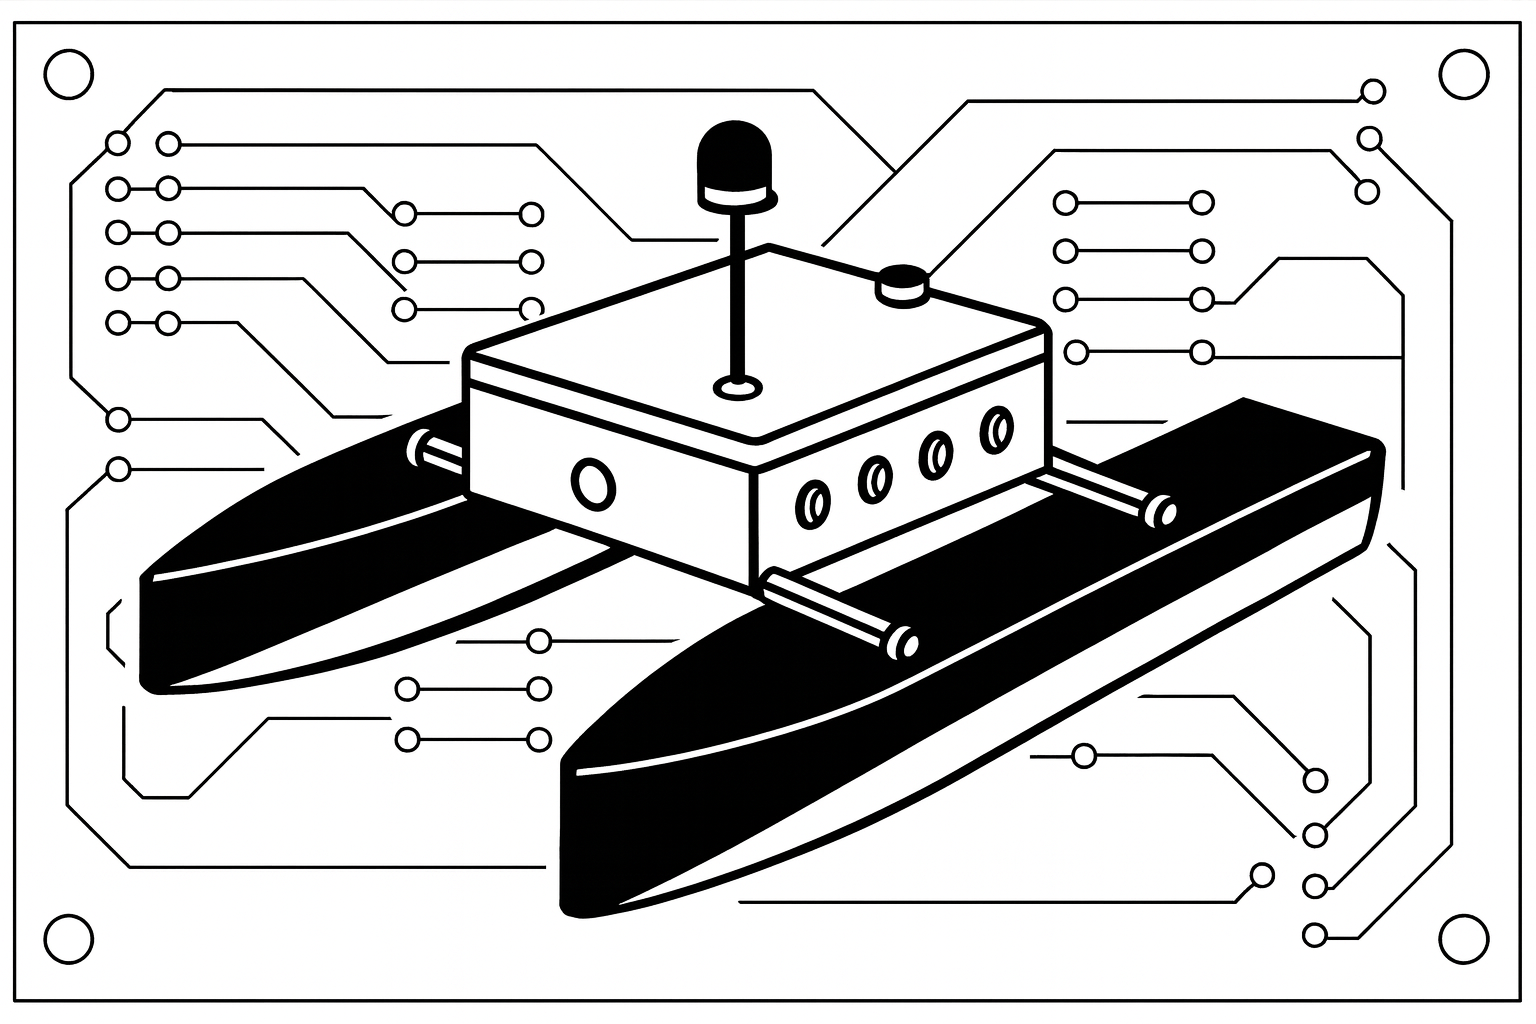
\includegraphics[width=12cm]{figuras/usv-2d.png}
	\end{center}\vspace{6pt}
	
	\begin{center}
		\LARGE
		\textbf{Sistema Ciberfísico para Controlo Autónomo de Embarcações \acrlong{usv}}\\\vspace{24pt}
		
		\Large
		ALEXANDRE MIGUEL CALEJO DE FIGUEIREDO\\
		\large
		Licenciado em Engenharia Informática e Multimédia\\\vspace{24pt}
		
		\normalsize
		Dissertação para obtenção do grau de mestre em Engenharia Informática e Multimédia
	\end{center}\vspace{12pt}
	
	\normalsize
	\noindent\hspace*{3.5cm}
	Orientadores:\\
	\noindent\hspace*{5.5cm}
	Professor Doutor Carlos Jorge de Sousa Gonçalves\\
	\noindent\hspace*{5.5cm}
	Professor Doutor Pedro Daniel Dinis Teodoro\\
	
	\noindent\hspace*{3.5cm}
	Júri:\\
	\noindent\hspace*{4.2cm}
	Presidente: Grau e Nome\\
	\noindent\hspace*{4.2cm}
	Vogais:\\
	\noindent\hspace*{5.5cm}
	Grau e Nome\\
	\noindent\hspace*{5.5cm}
	Grau e Nome\\
	
	\vfill
	\begin{center}
		\textbf{Setembro de 2025}
	\end{center}
\end{titlepage}

% Page with no page number
\thispagestyle{empty} % Para não colocar número de página

\begin{titlepage}
	\vspace*{1cm}	
	\begin{center}
		\LARGE
		\textbf{Sistema Ciberfísico para Controlo Autónomo de Embarcações \acrlong{usv}}\\\vspace{36pt}
	\end{center}\vfill

	\begin{center}
		\Large
		ALEXANDRE MIGUEL CALEJO DE FIGUEIREDO\\
		\large
		Licenciado em Engenharia Informática e Multimédia
	\end{center}\vfill

	\begin{center}
		\normalsize
        Dissertação para obtenção do grau de mestre em Engenharia Informática e Multimédia
	\end{center}\vfill
	
	\normalsize
	\noindent\hspace*{3.5cm}
	Orientador(es):\\
	\noindent\hspace*{5.5cm}
	  Professor Doutor Carlos Jorge de Sousa Gonçalves, ISEL\\
	\noindent\hspace*{5.5cm}
	Professor Doutor Pedro Daniel Dinis Teodoro, ENIDH\\
	
	\noindent\hspace*{3.5cm}
	Júri:\\
	\noindent\hspace*{4.2cm}
	Presidente: Grau e Nome, Afiliação\\
	\noindent\hspace*{4.2cm}
	Vogais:\\
	\noindent\hspace*{5.5cm}
	Grau e Nome, Afiliação\\
	\noindent\hspace*{5.5cm}
	Grau e Nome, Afiliação\\
	
	\vfill
	\begin{center}
		\textbf{Setembro de 2025}
	\end{center}
\end{titlepage}

% Page with no page number
\thispagestyle{empty} % Para não colocar número de página

% Page with no page number
\thispagestyle{empty} % Para não colocar número de página

\linespread{1.3}









\frontmatter % Inicialização da paginação (números romanos)
\newpage
\vspace*{\fill}
\begin{flushright}
\textit{"O cientista não procura um resultado imediato. Ele não espera que as suas ideias avançadas sejam prontamente aceites. O seu trabalho é lançar a base para aqueles que virão."} \\
--- Nikola Tesla
\end{flushright}
\vspace*{\fill}

\chapter{Agradecimentos}

Em primeiro lugar, quero expressar a minha profunda gratidão ao \acrfull{isel}, instituição que foi a minha casa ao longo de cinco anos (Licenciatura e Mestrado). Aqui encontrei não só os maiores desafios académicos da minha vida, mas também oportunidades únicas de crescimento pessoal e profissional. Foram muitas noites mal dormidas, momentos de frustração e superação, mas também conquistas que culminaram na realização deste \acrfull{tfm}.  

Agradeço igualmente à \acrfull{enidh}, que nos últimos meses se tornou a minha segunda casa, disponibilizando não apenas as condições necessárias para o desenvolvimento deste trabalho, mas também a embarcação e os espaços para ensaios. Graças a esta colaboração foi possível participar no exercício \gls{rex25}, um subevento do \gls{repmus25}, validando o protótipo em ambiente real.  

Quero também agradecer à Marinha Portuguesa e à Escola Naval pela oportunidade de integrar o \gls{repmus25} e o \gls{rex25}, onde este trabalho pôde ser colocado à prova em cenários operacionais exigentes. Esta experiência representou um marco na validação prática do sistema e um reconhecimento da importância de iniciativas académicas em contextos reais.  

Um agradecimento muito especial ao Professor Carlos Gonçalves, pela orientação incansável ao longo da licenciatura e do mestrado. O seu rigor, dedicação e espírito de exigência foram fundamentais para a conclusão deste percurso. Recordo as inúmeras noites no \gls{isel}, que se prolongavam até tarde, e que foram decisivas para transformar ideias em resultados concretos.  

Agradeço igualmente ao Professor Pedro Teodoro, pelo apoio na compreensão de conceitos ligados às embarcações e pela disponibilização da infraestrutura e embarcação necessárias para a realização dos testes.  

À minha família, em particular aos meus pais, agradeço por estarem sempre presentes e pelo apoio incondicional em todos os momentos. Sem o vosso incentivo e confiança, nada disto teria sido possível.  

Aos colegas e amigos que me acompanharam ao longo desta jornada académica, deixo também um sincero agradecimento. Foram muitas as vezes em que tive de recusar convites ou abdicar de momentos convosco devido às exigências deste mestrado, mas o vosso apoio e compreensão foram fundamentais para chegar até aqui.  

Um agradecimento também à minha empresa, Critical Techworks, pela flexibilidade e pelo apoio concedido durante os dois anos de mestrado. A possibilidade de conciliar a vida profissional com os estudos foi crucial para tornar este percurso viável.  

Finalmente, agradeço a mim próprio. Conciliar um mestrado com uma carreira profissional como trabalhador-estudante foi uma tarefa exigente e, por vezes, desgastante. No entanto, este trabalho é também prova de que, com esforço, dedicação e resiliência, é possível alcançar qualquer objetivo. Agradeço a mim por acreditar, por não desistir e por ser fiel a este caminho até ao fim.

\vspace*{\fill}
\begin{flushright}
\textit{"Conseguimos! Conseguimos, Portugal, Lisboa! Esperávamos, desejávamos, conseguimos! Vitória!"} \\
--- Doutor Marcelo Rebelo de Sousa
\end{flushright}
\vspace*{\fill}
% !TeX spellcheck = pt_PT2

\chapter{Declaração de integridade}

Declaro que este trabalho é o resultado da minha investigação pessoal e independente. O seu conteúdo é original e todas as fontes listadas nas referências bibliográficas foram consultadas e estão devidamente mencionadas no texto. Mais declaro que todas as referências científicas e técnicas relevantes para o desenvolvimento do trabalho estão devidamente citadas e constam das referências bibliográficas.\vspace{24pt}

\begin{center}
	O autor\\\vspace{24pt}
	\rule{8cm}{.3pt}\\
	Lisboa, 30 de setembro de 2025
\end{center}

% !TeX spellcheck = pt_PT2

\chapter{Resumo}

O trabalho final de mestrado apresentado neste relatório descreve o desenvolvimento de um sistema ciberfísico para controlo autónomo de embarcações do tipo \acrfull{usv}. O sistema foi concebido de forma modular, expansível e orientado para a integração de múltiplos motores, sensores e interfaces de comunicação, assegurando robustez e adaptabilidade a diferentes cenários operacionais.

A arquitetura proposta baseia-se na utilização de um microcontrolador \gls{esp32} com suporte nativo a \gls{i2c}, \gls{uart} e \gls{lora}, para controlo dos diferentes módulos, incluindo sensores e atuadores. Entre os principais módulos incluem-se: i) propulsores \emph{brushless} controlados por \acrfull{esc}, capazes de fornecer empuxo bidirecional; ii) um \acrfull{imu}, que fornece medições de \emph{yaw}, \emph{pitch} e \emph{roll} para garantir a estabilidade e a correção de trajetória; iii) um recetor \acrfull{gps}, responsável pela navegação precisa através de coordenadas geoespaciais; e iv) um módulo de comunicação \acrfull{lora}, que assegura telemetria de longo alcance e receção de rotas em tempo real com baixo consumo energético.

Do ponto de vista de \emph{software}, a solução foi estruturada em bibliotecas independentes que encapsulam funções de propulsão, sensorização, comunicação e controlo. Esta abordagem promove a reutilização de código, facilita a manutenção e garante a escalabilidade do sistema. A comunicação foi otimizada através do uso de \emph{Protocol Buffers} (\emph{Protobuf}), reduzindo significativamente o tempo de transmissão (\gls{toa}) em mensagens \acrfull{lora}, o que contribui para maior eficiência energética, menor probabilidade de colisões e aumento do alcance efetivo.

A validação experimental incluiu testes incrementais de \emph{hardware} e \emph{software}, desde o controlo isolado de propulsores até à integração de todos os módulos num protótipo funcional. Os resultados demonstraram a capacidade do sistema em seguir rotas definidas por \emph{waypoints} \acrfull{gps}, armazenar dados de telemetria e operar em modo manual ou automático.

Conclui-se que o sistema desenvolvido constitui uma base sólida para futuras evoluções em \acrfull{usv}, nomeadamente a aplicação de controladores avançados (\acrfull{pid} ou \acrfull{lqr}), a integração em plataformas marítimas de maior escala, e a utilização em cenários reais de monitorização ambiental, investigação científica e operações costeiras.

\vspace{-0.5cm}
\palavraschave{Palavras-chave: \gls{usv}; Sistemas Ciberfísicos; \gls{lora}; \gls{esp32}; Navegação Autónoma.}

\chapter*{Abstract}

This master's dissertation presents the development of a cyber-physical system for the autonomous control of Unmanned Surface Vehicles (\acrfull{usv}). The system was designed to be modular, extensible, and oriented towards the integration of multiple motors, sensors, and communication interfaces, ensuring robustness and adaptability to different operational scenarios.  

The proposed architecture is based on an \gls{esp32} microcontroller with native support for \gls{i2c}, \gls{uart}, and \gls{lora}, responsible for controlling various modules, including sensors and actuators. The main modules include: i) brushless thrusters controlled by \acrfull{esc}, capable of providing bidirectional thrust; ii) an \acrfull{imu}, supplying yaw, pitch, and roll measurements to guarantee stability and trajectory correction; iii) a \acrfull{gps} receiver, enabling accurate navigation through geospatial coordinates; and iv) a \gls{lora}-based communication module, providing long-range telemetry and real-time route updates with low energy consumption.  

From the \emph{software} perspective, the solution was structured into independent libraries that encapsulate propulsion, sensing, communication, and control functionalities. This modular approach fosters code reusability, simplifies maintenance, and ensures system scalability. Communication efficiency was enhanced by employing \emph{Protocol Buffers} (\emph{Protobuf}), which significantly reduced the \gls{toa} of \gls{lora} messages, leading to higher energy efficiency, lower collision probability, and increased effective range.  

Experimental validation included incremental \emph{hardware} and \emph{software} testing, ranging from isolated thruster control to the full integration of all modules into a functional prototype. The results demonstrated the system's ability to follow routes defined by \acrfull{gps} waypoints, store telemetry data, and operate in both manual and autonomous modes.  

It is concluded that the developed system provides a solid foundation for future advancements in \gls{usv}, particularly in the application of advanced controllers (\acrfull{pid} or \acrfull{lqr}), integration into larger-scale maritime platforms, and deployment in real-world scenarios such as environmental monitoring, scientific research, and coastal operations.

\keywords{\gls{usv}; Cyber-Physical Systems; \gls{lora}; \gls{esp32}; Autonomous Navigation.}


\renewcommand{\contentsname}{Índice de Conteúdos}
\tableofcontents

\addcontentsline{toc}{chapter}{Índice de Conteúdos}

\renewcommand{\listfigurename}{Índice de Figuras}
\listoffigures
\addcontentsline{toc}{chapter}{Índice de Figuras}

\renewcommand{\listtablename}{Índice de Tabelas}
\listoftables
\addcontentsline{toc}{chapter}{Índice de Tabelas}

\renewcommand{\lstlistlistingname}{Índice de Listagens}
\lstlistoflistings
\addcontentsline{toc}{chapter}{Índice de Listagens}
\renewcommand{\lstlistingname}{Listagem}

\renewcommand{\glossaryname}{Índice de Acrónimos}
\printglossary
\addcontentsline{toc}{chapter}{Índice de Acrónimos}

% !TeX spellcheck = pt_PT2

\newacronym{usv}{USV}{\emph{Unmanned Surface Vehicle}}
\newacronym{imu}{IMU}{\emph{Inertial Measurement Unit}}
\newacronym{gps}{GPS}{\emph{Global Positioning System}}
\newacronym{lora}{LoRa}{\emph{Long Range}}
\newacronym{tfm}{TFM}{Tese Final de Mestrado}
\newacronym{pwm}{PWM}{\emph{Pulse Width Modulation}}
\newacronym{i2c}{I2C}{\emph{Inter-Integrated Circuit}}
\newacronym{uart}{UART}{\emph{Universal Asynchronous Receiver/Transmitter}}
\newacronym{spi}{SPI}{\emph{Serial Peripheral Interface}}
\newacronym{dc}{DC}{\emph{Direct Current}}
\newacronym{pcb}{PCB}{\emph{Printed Circuit Board}}
\newacronym{esc}{ESC}{\emph{Electronic Speed Controller}}
\newacronym{esp32}{ESP32}{\emph{Espressif32}}
\newacronym{wifi}{Wi-Fi}{\emph{Wireless Fidelity}}
\newacronym{oled}{OLED}{\emph{Organic Light-Emitting Diode}}
\newacronym{esp-idf}{ESP-IDF}{\emph{Espressif IoT Development Framework}}
\newacronym{uml}{UML}{\emph{Unified Modeling Language}}
\newacronym{nmea}{NMEA}{\emph{National Marine Electronics Association}}
\newacronym{repmus25}{REPMUS25}{\emph{Robotic Experimentation and Prototyping using Maritime Uncrewed Systems 2025}}
\newacronym{rex25}{Naval-REX25}{\emph{Naval-Robotics Exercise 2025}}
\newacronym{html}{HTML}{\emph{Hyper Text Markup Language}}
\newacronym{zee}{ZEE}{Zona Económica Exclusiva}
\newacronym{pid}{PID}{\emph{Proportional-Integral-Derivative}}
\newacronym{lqr}{LQR}{\emph{Linear Quadratic Regulator}}
\newacronym{asv}{ASV}{\emph{Autonomous Surface Vehicle}}
\newacronym{toa}{ToA}{\emph{Time on Air}}
\newacronym{led}{LED}{\emph{Light-Emitting Diode}}
\newacronym{isel}{ISEL}{Instituto Superior de Engenharia de Lisboa}
\newacronym{enidh}{ENIDH}{Escola Superior Náutica Infante D. Henrique}


\mainmatter % Reinicialização da paginação (números árabes)
% !TeX spellcheck = pt_PT2

% \chapter{Introdução}

% O presente \textit{template} \LaTeX\ foi elaborado de acordo com as regras de formatação aprovadas pelo CTC. Tenha em atenção que, de acordo com essas regras, o seu TFM não deve ultrapassar 150 páginas, excluindo eventuais anexos.

% Após deszipar o ficheiro \verb|TFM.zip| notará que existem três ficheiros, a saber: \verb|TFM.tex|, \verb|formatacao.tex| e \verb|bibdatabase.bib|. O primeiro é o ficheiro principal. É este o ficheiro a ser compilado para produzir o TFM. O segundo contém definições de formatação e o terceiro os dados das referências bibliográficas. Há também duas diretorias: \verb|figuras| e \verb|tex|, a primeira destinada a guardar todas as figuras do TFM e a segunda todos os ficheiros TEX essenciais à compilação do documento, incluindo um ficheiro TEX por cada capítulo.

% Se desejar iniciar-se como utilizador \LaTeX\ deve começar por instalar no computador uma versão do compilador adequada ao seu sistema operativo. No caso do Windows, um dos compiladores mais utilizados é o MikTeX, que pode ser instalado a partir do endereço:

% \begin{center}
% 	\url{http://miktex.org/}	
% \end{center}

% Os ficheiros TEX podem ser criados a partir de qualquer editor de texto, mas existem alguns desenvolvidos especificamente para esse fim. Um editor muito versátil é o TeXstudio, que pode ser descarregado a partir do endereço:

% \begin{center}
% 	\url{http://www.texstudio.org/}
% \end{center}

% Se não tem nenhuma noção de \LaTeX\ e deseja ter uma ideia de como o sistema funciona, veja o documento first-latex-doc.pdf, que pode ser descarregado a partir de:

% \begin{center}
% 	\url{https://ctan.org/tex-archive/info/first-latex-doc}
% \end{center}

% Um excelente manual do sistema está disponível gratuitamente em:

% \begin{center}
% 	\url{https://en.wikibooks.org/wiki/LaTeX}
% \end{center}

% O presente documento exemplifica o uso dos comandos para produzir as unidades de texto típicas de textos científicos, nomeadamente:

% \begin{enumerate}[noitemsep]
% 	\item figuras,
% 	\item tabelas,
% 	\item listas,
% 	\item equações matemáticas,
% 	\item bibliografia e sua referenciação. 
% \end{enumerate}

\chapter{Introdução}
\label{ch:introducao}

O presente \gls{tfm} tem como objetivo o desenvolvimento de um sistema ciberfísico para o controlo de veículos autónomos, concebido de forma genérica para abranger tanto plataformas terrestres como marítimas, sendo o caso de estudo deste \gls{tfm} a aplicação a um \gls{usv} com capacidade de navegação autónoma. O sistema a ser desenvolvido deverá ser capaz de controlar até quatro motores de forma independente, garantindo a manobrabilidade necessária para diferentes cenários de operação. Além disso, será integrado com um conjunto de sensores essenciais, incluindo: i) sensores de temperatura e humidade, para monitorização ambiental; ii) um \gls{imu}, responsável por medir e ajustar a orientação e aceleração do \gls{usv}; e iii) um \gls{gps}, para navegação precisa através de coordenadas geoespaciais.

Para permitir a comunicação de longo alcance, o sistema incluirá uma interface \gls{lora}, que viabilizará o envio de dados de telemetria e a receção de novas rotas de navegação de forma eficiente, mesmo em áreas remotas.

O protótipo desenvolvido deverá ser capaz de seguir autonomamente uma rota constituída por coordenadas \gls{gps} previamente definidas. Durante a navegação, o sistema armazenará os dados de telemetria, incluindo a posição e o estado da embarcação, em um cartão de memória, permitindo não apenas a posterior avaliação do desempenho do veículo, mas também o estudo detalhado da trajetória efetivamente seguida em comparação com a rota planeada.

\section{Motivação}
\label{sec:motivacao}

A motivação para o desenvolvimento deste trabalho surge da necessidade crescente de soluções tecnológicas que permitam explorar, monitorizar e intervir em ambientes marítimos de forma autónoma, segura e eficiente. Os \gls{usv} representam uma alternativa promissora a embarcações tripuladas em missões de risco ou em operações que requerem elevada precisão, contribuindo para áreas como a investigação científica, a monitorização ambiental, a defesa e a segurança marítima.  

Para além desta motivação aplicada, o trabalho insere-se num percurso académico e científico que começou com o desenvolvimento de um robô didático \cite{didactic-robot-thesis}, concebido para fins pedagógicos. Esse projeto permitiu consolidar conhecimentos fundamentais sobre controlo de movimento, integração de sensores e comunicação sem fios. Com base nessa experiência, emergiu a necessidade de validar, em contexto real e com maior complexidade, se os princípios teóricos e arquiteturais aplicados em ambientes laboratoriais são escaláveis e eficazes em sistemas ciberfísicos de maior dimensão. Assim, este \gls{tfm} não só visa propor uma solução tecnológica inovadora, como também demonstrar, através de validação experimental, que os conceitos previamente adquiridos podem ser aplicados com sucesso a um \gls{usv}.  

\section{Contextualização}
\label{sec:contextualizacao}

O desenvolvimento de veículos marítimos autónomos tem registado um crescimento acentuado a nível mundial \cite{gminsights-autonomous-marine-vehicle}, impulsionado pela necessidade de monitorização de ecossistemas marinhos, exploração de zonas remotas e apoio a operações de defesa. Em particular, Portugal, com a sua extensa \gls{zee}, apresenta um contexto altamente relevante para a adoção de tecnologias de robótica marítima.  

Os \gls{usv} baseados em propulsão elétrica, equipados com sensores e módulos de comunicação de longo alcance, têm-se afirmado como plataformas versáteis para missões de curta e média duração. No entanto, o elevado custo associado às soluções comerciais limita a sua utilização em contextos académicos e de investigação aplicada.  

Neste enquadramento, o presente trabalho resulta da colaboração entre o \gls{isel} e a \gls{enidh}, instituições que partilham o objetivo de promover soluções inovadoras e acessíveis no domínio da robótica marítima. Esta parceria não só viabilizou o desenvolvimento de um protótipo de baixo custo, modular e escalável, como também criou condições privilegiadas para a realização de ensaios práticos em ambiente real. Foi nesse âmbito que o sistema pôde ser testado no \gls{repmus25}, mais concretamente no subevento \gls{rex25}, da Marinha Portuguesa e Escola Naval, permitindo validar conceitos avançados de navegação autónoma e comunicação sem fios em condições operacionais próximas das que se encontram em missões reais \cite{isel-repmus, enidh-repmus, sapo-repmus}.

Todo o código desenvolvido neste \gls{tfm} encontra-se em um repositório remoto público (\emph{open source}) no GitHub \cite{github-usv}. Este processo assegurou a rastreabilidade das alterações, a organização das diferentes versões do código e a possibilidade de colaboração futura.

\section{Organização do Documento}
\label{sec:organizacao}

Este documento encontra-se estruturado em sete capítulos principais. O Capítulo \ref{ch:introducao} apresenta a introdução ao trabalho, incluindo a motivação, a contextualização e a organização do \gls{tfm}. O Capítulo \ref{ch:estadodaarte} descreve o estado da arte, explorando soluções existentes e antecedentes relevantes, incluindo o projeto do robô didático que serviu de base conceptual. O Capítulo \ref{ch:modeloProposto} define o modelo proposto, os requisitos do sistema e a abordagem metodológica adotada. O Capítulo \ref{ch:arquitetura} detalha a arquitetura do sistema, abrangendo os módulos de \emph{hardware} e \emph{software} necessários para a operação do \gls{usv}. O Capítulo \ref{ch:implementacao} aborda a implementação prática, descrevendo o processo de integração e as soluções desenvolvidas. O Capítulo \ref{ch:validacaoTestes} apresenta a validação e os testes realizados, desde ensaios incrementais até à validação em ambiente real no exercício internacional \gls{repmus25}. Por fim, o Capítulo \ref{ch:conclusoesTrabalhoFuturo} apresenta as conclusões obtidas e as perspetivas para trabalho futuro, destacando potenciais evoluções e aplicações do sistema.

% !TeX spellcheck = pt_PT2

\chapter{Estado da Arte} \label{ch:estadodaarte}

O estado da arte apresentado neste capítulo tem como objetivo contextualizar o desenvolvimento de \gls{usv} no panorama atual da robótica marítima. São discutidas as principais soluções de propulsão, desde abordagens baseadas em energias renováveis até plataformas motorizadas de alto desempenho, destacando as respetivas vantagens, limitações e áreas de aplicação. Adicionalmente, é feita uma ponte com o trabalho realizado durante a licenciatura, o qual serviu de base conceptual e experimental para o presente \gls{tfm}. Esta análise fornece o enquadramento necessário para compreender a evolução tecnológica nesta área e justifica as opções adotadas no desenvolvimento do protótipo proposto.

\section{Trabalho Relacionado} 
\label{sec:trabalhorelacionado}

O desenvolvimento de \gls{usv} tem atraído crescente atenção devido à sua relevância em operações de monitorização, recolha de dados e exploração de ambientes marítimos. Estas plataformas permitem realizar missões de forma segura e eficiente em áreas de difícil acesso ou potencialmente perigosas para embarcações tripuladas, constituindo uma solução cada vez mais valorizada em contextos científicos, ambientais e de defesa.  

Entre as alternativas de propulsão destacam-se soluções que dispensam motores convencionais. O \emph{Wave Glider}, desenvolvido pela Liquid Robotics \cite{wave-glider}, utiliza a energia das ondas para se deslocar de forma contínua e passiva, sendo particularmente adequado para missões de longa duração com baixo consumo energético. A Figura~\ref{fig:wave-glider} ilustra o princípio de funcionamento do mecanismo de propulsão por ondas (Figura \ref{fig:wave-glider} (A)) e a estrutura de superfície (Figura \ref{fig:wave-glider} (B)) responsável por garantir flutuabilidade e suporte para a instalação de sensores e antenas.

\begin{figure}[H]
    \centering
    \begin{minipage}{0.45\linewidth}
        \centering
        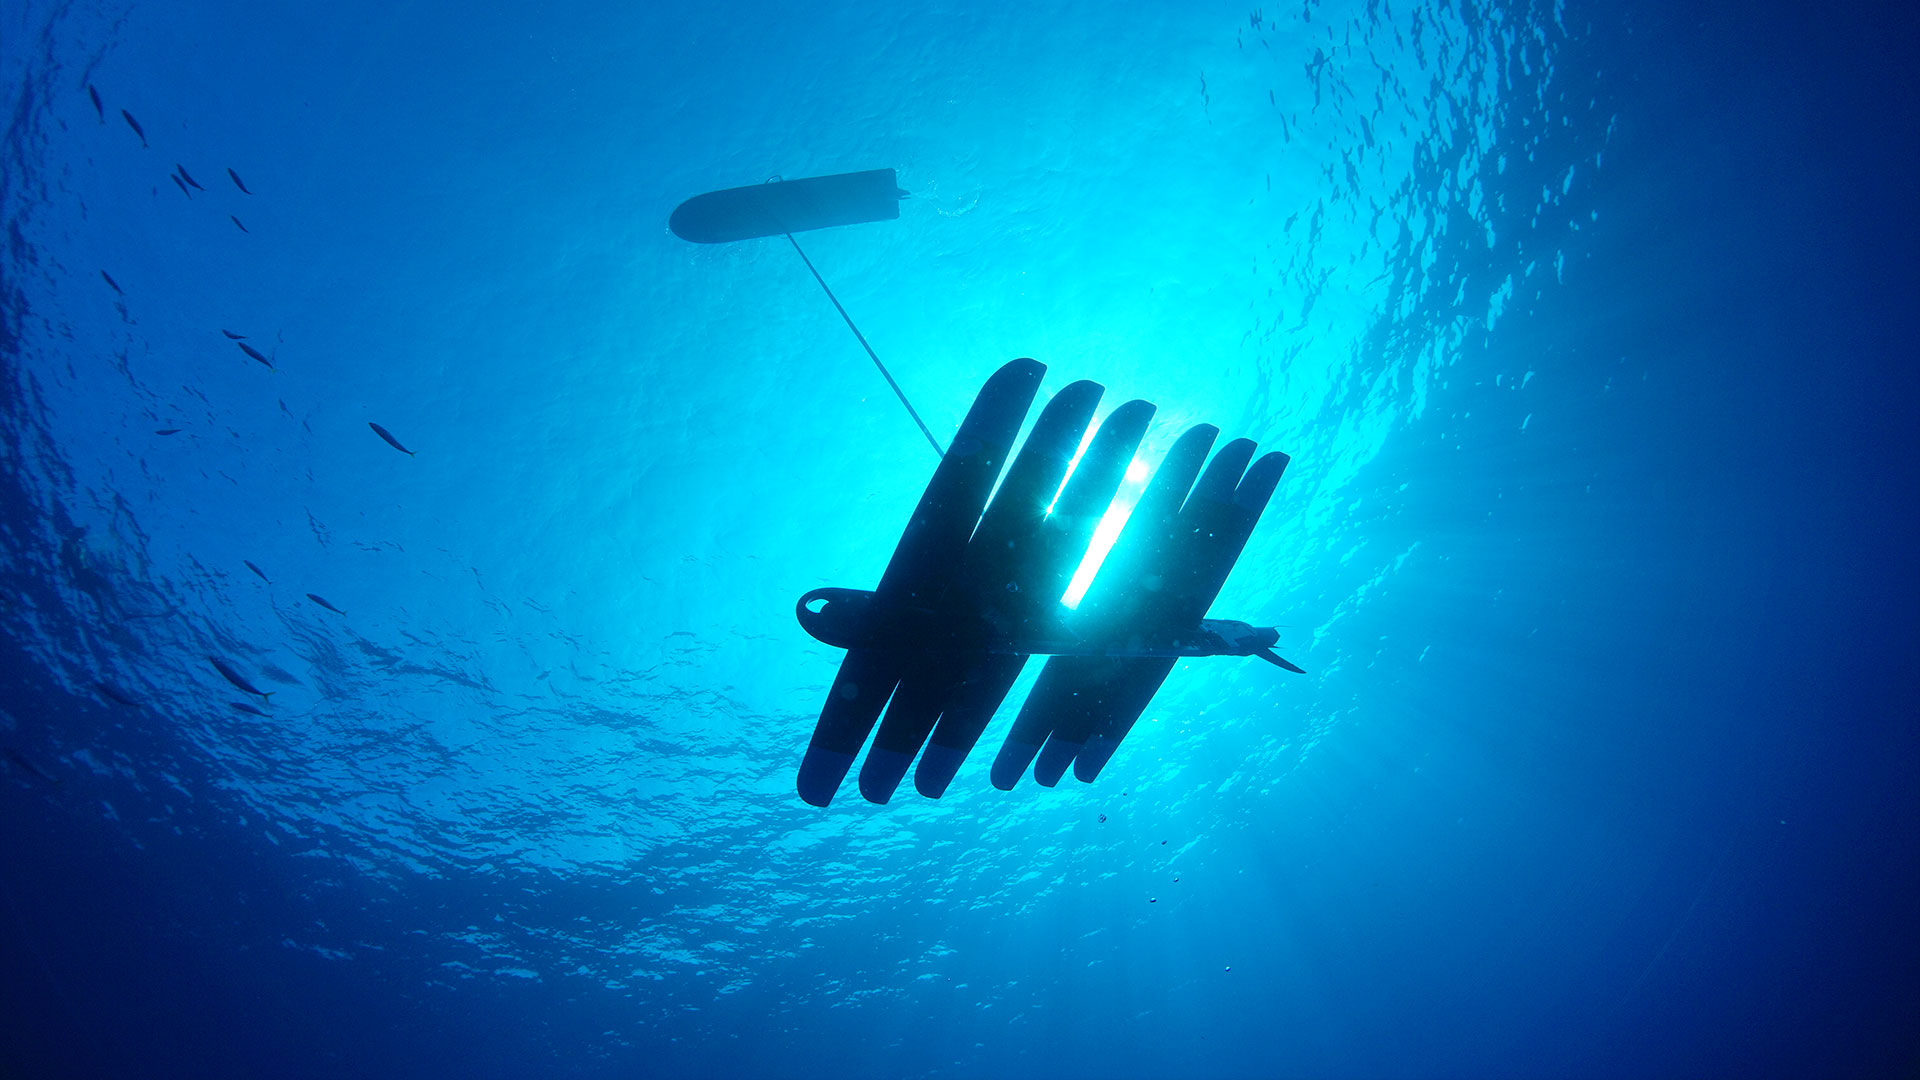
\includegraphics[width=\linewidth]{figuras/wave-glider.jpg}
        \caption*{(A) Mecanismo de propulsão por ondas}
    \end{minipage}
    \hfill
    \begin{minipage}{0.45\linewidth}
        \centering
        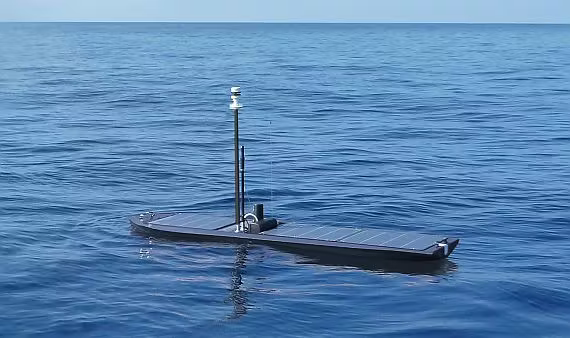
\includegraphics[width=\linewidth]{figuras/wave-glider2.png}
        \caption*{(B) Estrutura da superfície}
    \end{minipage}
    \caption[\gls{usv} Liquid Robotics Wave Glider]{\gls{usv} Liquid Robotics Wave Glider \cite{wave-glider}}
    \label{fig:wave-glider}
\end{figure}

Outra abordagem alternativa é o \emph{Saildrone} \cite{saildrone}, representado na Figura \ref{fig:saildrone}, que recorre à propulsão à vela. 

\begin{figure}[H]
    \centering
    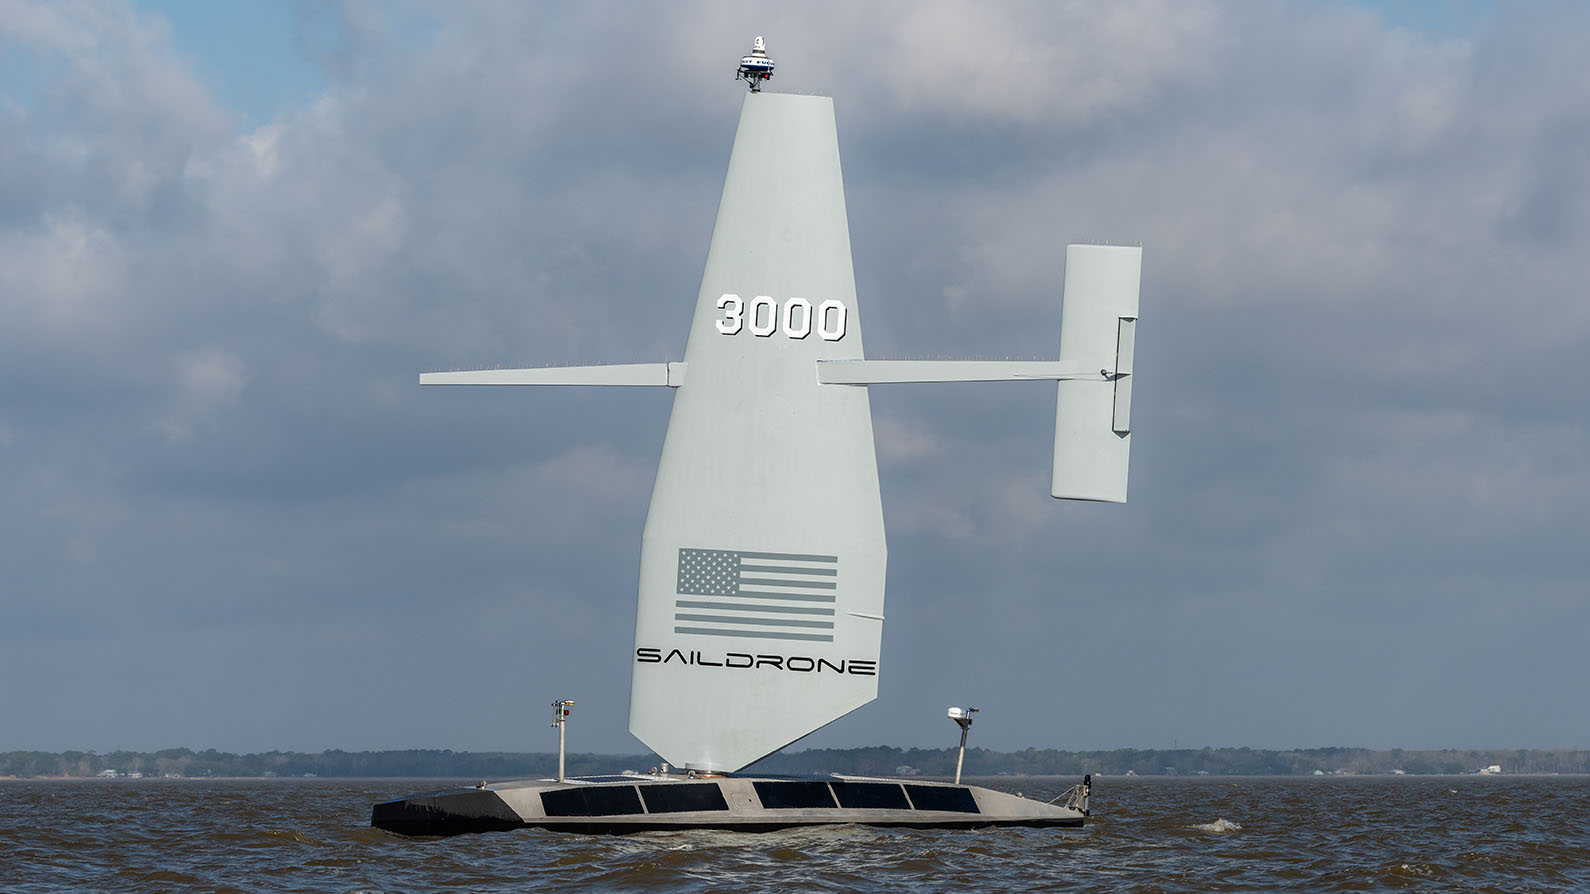
\includegraphics[width=0.5\linewidth]{saildrone-usv.jpg}
    \caption[\gls{usv} Saildrone]{\gls{usv} Saildrone \cite{saildrone}}
    \label{fig:saildrone}
\end{figure}

Este tipo de \gls{usv} tem sido amplamente utilizado em campanhas de monitorização oceânica de larga escala, tirando partido da elevada autonomia oferecida pela energia eólica.  

Apesar das vantagens associadas à utilização de fontes renováveis, as \gls{usv} motorizadas oferecem maior controlo de navegação, velocidade e manobrabilidade, características essenciais em ambientes de correntes variáveis ou condições marítimas adversas. Um exemplo relevante é o SeaRobotics SR-Surveyor \cite{sr-surveyor-class}, amplamente utilizado em levantamentos hidrográficos e mapeamento subaquático, equipado com sonar multifeixe para operações precisas em ambientes costeiros e portuários.  

\begin{figure}[H]
    \centering
    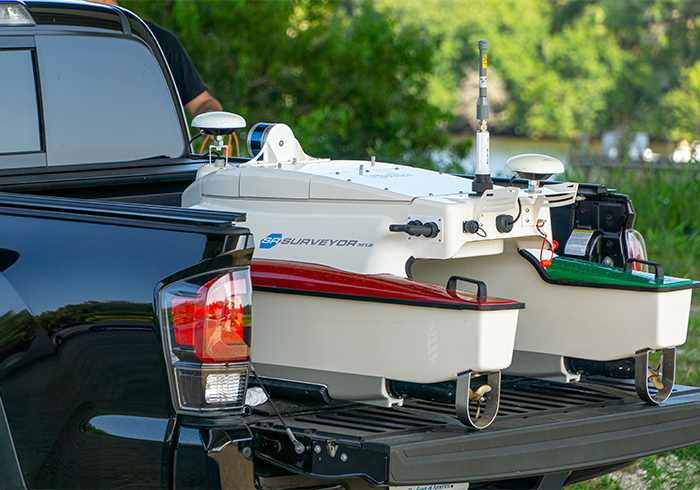
\includegraphics[width=0.5\linewidth]{figuras/sr-surveyorm18-truck-bed.jpg}
    \caption[SeaRobotics SR-Surveyor]{SeaRobotics SR-Surveyor \cite{sr-surveyor-class}}
    \label{fig:sr-surveyor-carrinha}
\end{figure}

A Figura \ref{fig:c-cat-3-asv} apresenta outro exemplo, o \gls{asv} (subclasse de \gls{usv}) Global's C-Cat 3 \cite{c-cat-3-asv}.

\begin{figure}[H]
    \centering
    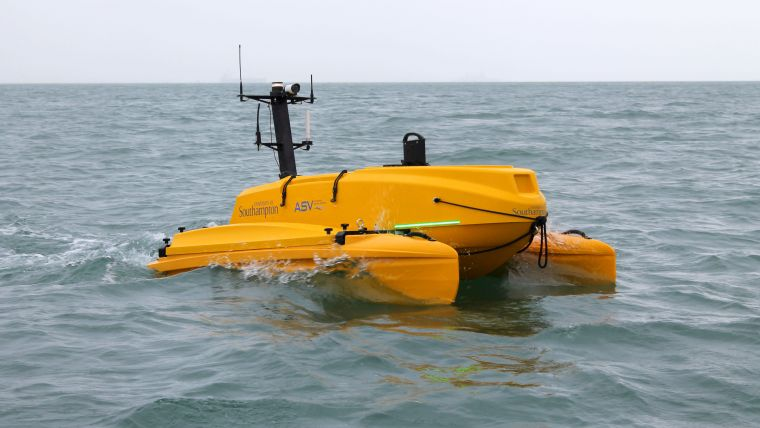
\includegraphics[width=0.5\linewidth]{figuras/c-cat3.jpeg}
    \caption[\gls{asv} Global C-Cat 3]{\gls{asv} Global C-Cat 3 \cite{c-cat-3-asv}}
    \label{fig:c-cat-3-asv}
\end{figure}

O C-Cat~3 \cite{c-cat-3-asv} é um \gls{usv} de dimensões compactas, propulsionado por motor elétrico, projetado para operar em águas pouco profundas. A sua conceção modular e elevada manobrabilidade tornam-no particularmente adequado para missões de monitorização ambiental, levantamentos batimétricos e outras aplicações científicas ou de reconhecimento costeiro.

Também em Portugal têm surgido iniciativas relevantes, como o projeto Sea2Future \cite{sea2future,sea2future2}, desenvolvido pela Escola Superior Náutica Infante D. Henrique, que, conforme ilustrado na Figura \ref{fig:sea2future}, explora o potencial dos \gls{usv} motorizados em cenários de resgate e recolha de dados ambientais.

\begin{figure}[H]
    \centering
    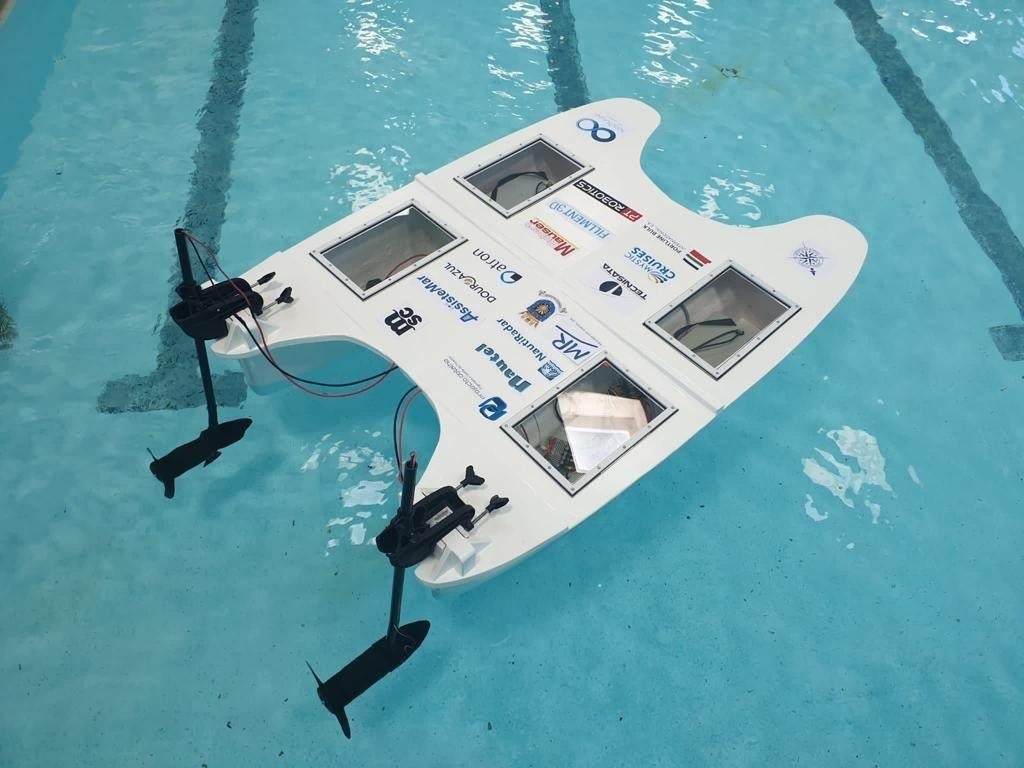
\includegraphics[width=0.5\linewidth]{figuras/sea2future.jpg}
    \caption[\gls{usv} do projeto Sea2Future]{\gls{usv} do projeto Sea2Future \cite{sea2future,sea2future2}}
    \label{fig:sea2future}
\end{figure}

Embora tecnologicamente avançadas, estas soluções comerciais apresentam custos elevados, frequentemente na ordem de centenas de milhares de euros. A aquisição e manutenção de plataformas como o SR-Surveyor ou o C-Cat 3 podem atingir valores próximos de meio milhão de euros, dependendo do conjunto de sensores e da robustez estrutural requerida para operar em ambientes marítimos adversos.  

Nos últimos anos, os avanços tecnológicos em sistemas de controlo e sensorização têm impulsionado o desenvolvimento de \gls{usv} mais acessíveis e modulares. Destaca-se o controlo independente de múltiplos motores, aliado à integração de sensores como \gls{gps}, \gls{imu} e sensores ambientais, que tornam estas plataformas cada vez mais autossuficientes e precisas, abrindo caminho para aplicações em larga escala em monitorização costeira, exploração científica e operações de segurança.

\section{\emph{Background}} 
\label{sec:background}

Durante o percurso académico da licenciatura, foi desenvolvido um projeto descrito em \cite{didactic-robot-thesis}, cujo objetivo principal consistiu na criação de um ambiente didático orientado para a exploração de conceitos fundamentais em robótica, como o controlo de movimento, a comunicação sem fios e a programação em C e Java. O resultado deste trabalho foi um protótipo funcional de robô didático, concebido como uma ferramenta pedagógica eficaz.  

A arquitetura do sistema, apresentada em \cite{didactic-robot-thesis} e ilustrada na Figura \ref{fig:arquitetura-robo-didatico}, foi concebida segundo uma abordagem modular e expansível. Esta estrutura permitia a integração de até quatro motores (localizados na parte direita da figura), incluía os módulos de comunicação (representados no centro) e os módulos de sensorização (à esquerda), possibilitando a implementação e validação de diferentes configurações de forma flexível e adaptável.

\begin{figure}[H]
    \centering
    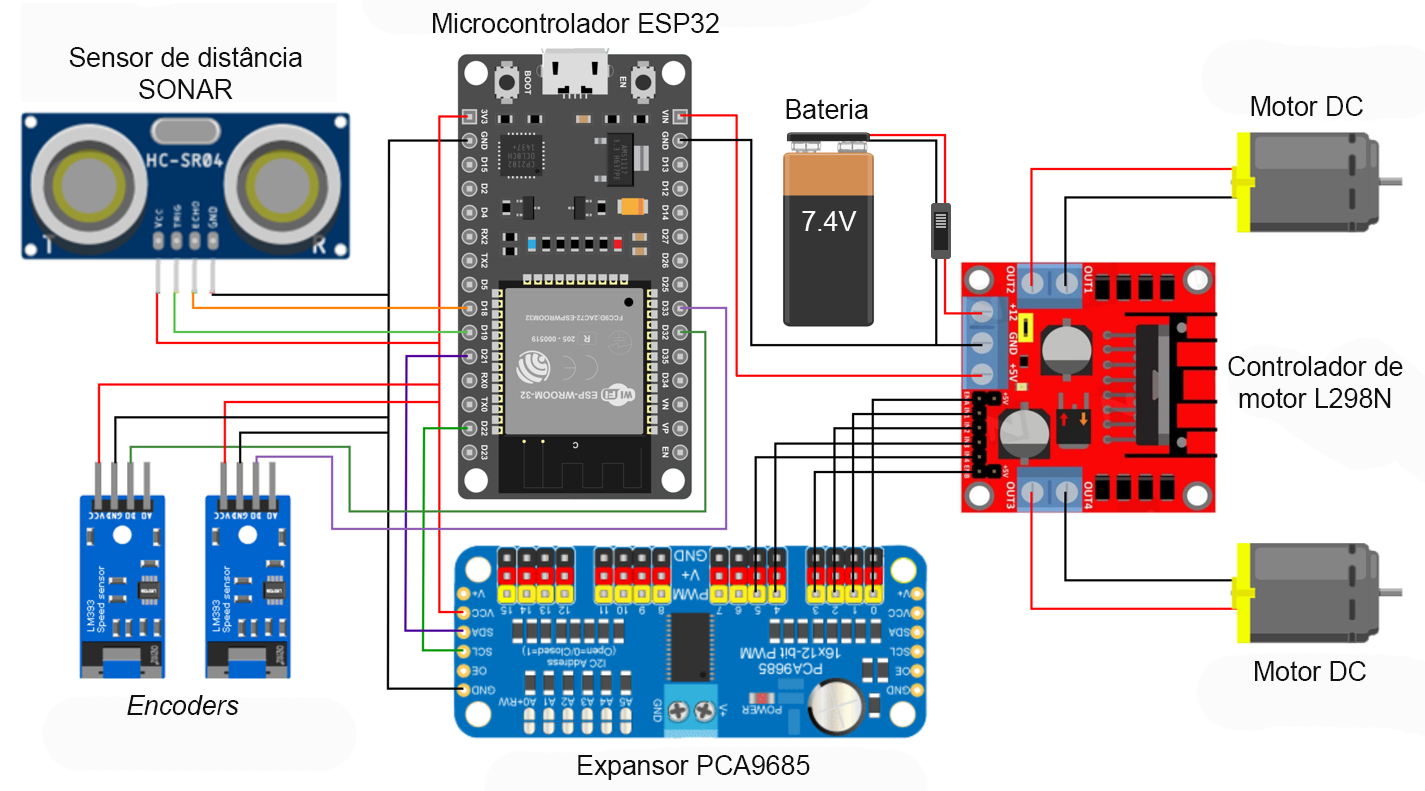
\includegraphics[width=0.95\linewidth]{figuras/arquitetura_robo_didatico.png}
    \caption[Arquitetura do Robô Didático]{Arquitetura do Robô Didático \cite{didactic-robot-thesis}}
    \label{fig:arquitetura-robo-didatico}
\end{figure}

O projeto culminou na construção de um protótipo físico, ilustrado na Figura \ref{fig:estrutura-robo-didatico}, que materializou a arquitetura proposta e demonstrou em ambiente real a integração de motores, sensores e módulos de comunicação. Esta validação experimental confirmou a viabilidade da abordagem modular, destacando a facilidade de substituição ou expansão de componentes.  

\begin{figure}[H]
    \centering
    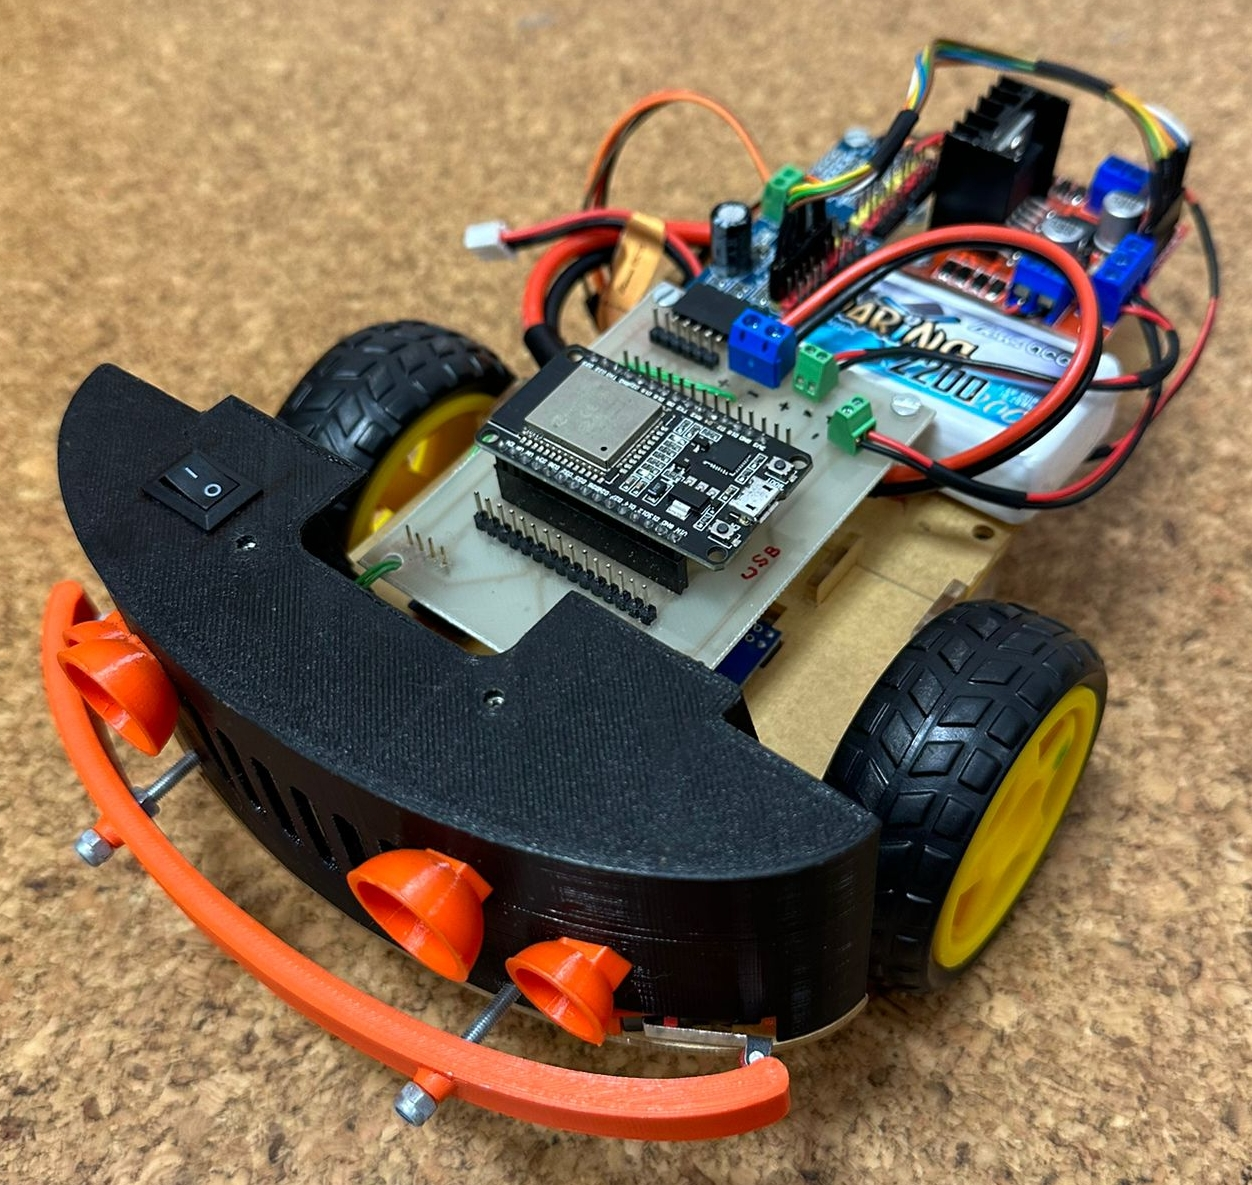
\includegraphics[width=0.5\linewidth]{figuras/robot-didatico.jpg}
    \caption[Estrutura final do Robô Didático]{Estrutura final do Robô Didático \cite{didactic-robot-thesis}}
    \label{fig:estrutura-robo-didatico}
\end{figure}

Um dos elementos centrais desta arquitetura era o controlador de motores, que assegurava a ligação entre a bateria principal e os diferentes atuadores. Este módulo não só suportava uma ampla gama de tensões de entrada, adequada para motores de diferentes características, como também fornecia uma saída regulada para o microcontrolador, simplificando a gestão energética do sistema. A presença de um interruptor dedicado entre a bateria e o controlador permitia desligar rapidamente todo o sistema em situações de teste ou emergência, reforçando a segurança operacional.  

O presente \gls{tfm} surge como uma evolução natural deste projeto, aplicando e expandindo os conceitos adquiridos para o desenvolvimento de um \gls{usv} com capacidade de navegação autónoma. Embora a lógica base da arquitetura tenha sido mantida, nomeadamente a utilização do barramento \gls{i2c} como interface principal de comunicação, foram realizadas adaptações relevantes. Os motores \gls{dc} do robô didático foram substituídos por propulsores \emph{brushless}, controlados por \gls{esc}, mais adequados ao ambiente marítimo.  

Adicionalmente, foram removidos sensores como o sonar e os encoders, que no contexto terrestre permitiam estimar a distância percorrida a partir do número de rotações da roda. No caso de um \gls{usv}, esta abordagem revela-se inviável, pois fatores externos como correntes, vento ou turbulência influenciam a relação entre rotações do propulsor e distância efetivamente percorrida. Para superar esta limitação, os encoders foram substituídos por um \gls{imu} e por um \gls{gps}, que fornecem medições absolutas de aceleração e orientação, permitindo estimar com maior precisão o movimento do veículo em ambiente marítimo.  

Assim, o trabalho desenvolvido na licenciatura serviu de alicerce conceptual e experimental para o presente \gls{tfm}, onde a arquitetura foi adaptada a um contexto mais exigente, integrando sensores e atuadores adequados às particularidades da navegação marítima.

\chapter{Modelo Proposto}
\label{ch:modeloProposto}

O modelo proposto neste \gls{tfm} consiste no desenvolvimento de um sistema ciberfísico para o controlo autónomo de embarcações do tipo \gls{usv}, concebido de forma modular e expansível. A modularidade é garantida pela utilização do barramento \gls{i2c} de comunicação entre os diferentes módulos de \emph{hardware}. A escolha do \gls{i2c} como base do sistema justifica-se pela sua simplicidade de implementação, baixo número de ligações necessárias e pela possibilidade de integrar múltiplos dispositivos no mesmo barramento através da atribuição de endereços únicos. Esta abordagem garante escalabilidade, permitindo a integração de novos sensores, atuadores, ou até mesmo diferentes microcontroladores, desde que estes suportem \gls{i2c}, sem alterações profundas na arquitetura.

De forma a apresentar esta proposta de forma estruturada, este capítulo encontra-se organizado em duas secções. Na Secção~\ref{sec:requisitos} são descritos os requisitos funcionais e não funcionais que orientam o desenvolvimento do sistema, identificando as funcionalidades essenciais e as propriedades globais de desempenho e escalabilidade. Na Secção~\ref{sec:abordagem} é detalhada a abordagem modular seguida, apresentando os principais módulos de \emph{hardware} e \emph{software} que compõem o sistema, bem como as suas interações. Esta estrutura permite compreender de forma clara tanto as bases conceptuais como a implementação prática do modelo proposto.

\section{Requisitos}
\label{sec:requisitos}

Os Requisitos Funcionais correspondem a descrições formais e detalhadas das funcionalidades que um sistema deve disponibilizar, especificando as ações que este deve ser capaz de executar e a forma como deve responder às diferentes interações do utilizador ou de outros sistemas.  

Por sua vez, os Requisitos Não Funcionais referem-se a propriedades globais do sistema que não estão diretamente associadas a uma funcionalidade específica, mas que condicionam o seu comportamento e qualidade de operação. Entre estes incluem-se aspetos como o desempenho, a segurança, a usabilidade, a escalabilidade e a fiabilidade, que são determinantes para garantir a robustez e adequação da solução em cenários reais de utilização.

Os requisitos principais definidos para o sistema proposto neste \gls{tfm} são:

\begin{enumerate}
    \item O sistema deve utilizar comunicação de longo alcance baseada em tecnologia \gls{lora}, de forma a permitir telemetria e atualização de rotas em tempo real, mesmo em cenários remotos.  
    Requisito funcional, dado que descreve explicitamente uma ação que o sistema deve executar, isto é, a capacidade de estabelecer comunicação sem fios de longo alcance para troca de dados críticos com a estação de controlo.

    \item O sistema deve ser expansível através do barramento \gls{i2c}, assegurando a fácil integração de novos módulos.  
    Requisito não funcional, uma vez que não descreve uma funcionalidade direta do sistema, mas sim uma característica de extensibilidade e escalabilidade, que garante a adaptabilidade futura da arquitetura.  
\end{enumerate}

Desta forma, observa-se que o primeiro requisito define uma funcionalidade central para a operação do veículo, indispensável para o cumprimento dos objetivos de navegação autónoma e monitorização remota enquanto o segundo requisito reflete uma propriedade estrutural do sistema, relacionada com a sua capacidade de evolução e integração modular.

\section{Abordagem}
\label{sec:abordagem}

Para assegurar a operação autónoma, o sistema integra diferentes módulos, tal como apresentado na Figura \ref{fig:modulos-usv}. 

\begin{figure}[H]
  \centering
  \resizebox{0.8\textwidth}{!}{%
    % generated by Plantuml 1.2024.3       
\definecolor{plantucolor0000}{RGB}{241,241,241}
\definecolor{plantucolor0001}{RGB}{24,24,24}
\definecolor{plantucolor0002}{RGB}{0,0,0}
\definecolor{plantucolor0003}{RGB}{255,255,224}
\definecolor{plantucolor0004}{RGB}{173,216,230}
\definecolor{plantucolor0005}{RGB}{144,238,144}
\begin{tikzpicture}[yscale=-1
,pstyle0/.style={color=plantucolor0001,fill=plantucolor0000,line width=0.5pt}
,pstyle2/.style={color=plantucolor0001,fill=plantucolor0004,line width=0.5pt}
,pstyle3/.style={color=plantucolor0001,fill=plantucolor0005,line width=0.5pt}
,pstyle5/.style={color=plantucolor0001,line width=1.0pt}
,pstyle6/.style={color=plantucolor0001,fill=plantucolor0001,line width=1.0pt}
,pstyle7/.style={color=plantucolor0001,line width=1.0pt,dash pattern=on 7.0pt off 7.0pt}
]
\draw[pstyle0] (150pt,12pt) arc (180:270:5pt) -- (155pt,7pt) -- (302.6571pt,7pt) arc (270:360:5pt) -- (307.6571pt,12pt) -- (307.6571pt,41.0679pt) arc (0:90:5pt) -- (302.6571pt,46.0679pt) -- (155pt,46.0679pt) arc (90:180:5pt) -- (150pt,41.0679pt) -- cycle;
\node at (160pt,17pt)[below right,color=black]{Microcontrolador};
\draw[color=plantucolor0001,fill=plantucolor0003,line width=0.5pt] (7pt,112pt) arc (180:270:5pt) -- (12pt,107pt) -- (85.9636pt,107pt) arc (270:360:5pt) -- (90.9636pt,112pt) -- (90.9636pt,160.1358pt) arc (0:90:5pt) -- (85.9636pt,165.1358pt) -- (12pt,165.1358pt) arc (90:180:5pt) -- (7pt,160.1358pt) -- cycle;
\node at (17pt,117pt)[below right,color=black]{\textit{\guillemotleft comm\guillemotright }};
\node at (29.0524pt,136.0679pt)[below right,color=black]{LoRa};
\draw[pstyle2] (126pt,112pt) arc (180:270:5pt) -- (131pt,107pt) -- (207.4966pt,107pt) arc (270:360:5pt) -- (212.4966pt,112pt) -- (212.4966pt,160.1358pt) arc (0:90:5pt) -- (207.4966pt,165.1358pt) -- (131pt,165.1358pt) arc (90:180:5pt) -- (126pt,160.1358pt) -- cycle;
\node at (136pt,117pt)[below right,color=black]{\textit{\guillemotleft sensor\guillemotright }};
\node at (154.2637pt,136.0679pt)[below right,color=black]{GPS};
\draw[pstyle2] (247pt,112pt) arc (180:270:5pt) -- (252pt,107pt) -- (328.4966pt,107pt) arc (270:360:5pt) -- (333.4966pt,112pt) -- (333.4966pt,160.1358pt) arc (0:90:5pt) -- (328.4966pt,165.1358pt) -- (252pt,165.1358pt) arc (90:180:5pt) -- (247pt,160.1358pt) -- cycle;
\node at (257pt,117pt)[below right,color=black]{\textit{\guillemotleft sensor\guillemotright }};
\node at (274.1626pt,136.0679pt)[below right,color=black]{IMU};
\draw[pstyle0] (368pt,121.5pt) arc (180:270:5pt) -- (373pt,116.5pt) -- (425.0889pt,116.5pt) arc (270:360:5pt) -- (430.0889pt,121.5pt) -- (430.0889pt,150.5679pt) arc (0:90:5pt) -- (425.0889pt,155.5679pt) -- (373pt,155.5679pt) arc (90:180:5pt) -- (368pt,150.5679pt) -- cycle;
\node at (378pt,126.5pt)[below right,color=black]{PWM};
\draw[pstyle3] (291pt,259.5pt) arc (180:270:5pt) -- (296pt,254.5pt) -- (388.1143pt,254.5pt) arc (270:360:5pt) -- (393.1143pt,259.5pt) -- (393.1143pt,307.6358pt) arc (0:90:5pt) -- (388.1143pt,312.6358pt) -- (296pt,312.6358pt) arc (90:180:5pt) -- (291pt,307.6358pt) -- cycle;
\node at (301pt,264.5pt)[below right,color=black]{\textit{\guillemotleft actuator\guillemotright }};
\node at (311.3137pt,283.5679pt)[below right,color=black]{Motor 1};
\draw[pstyle3] (428pt,259.5pt) arc (180:270:5pt) -- (433pt,254.5pt) -- (525.1143pt,254.5pt) arc (270:360:5pt) -- (530.1143pt,259.5pt) -- (530.1143pt,307.6358pt) arc (0:90:5pt) -- (525.1143pt,312.6358pt) -- (433pt,312.6358pt) arc (90:180:5pt) -- (428pt,307.6358pt) -- cycle;
\node at (438pt,264.5pt)[below right,color=black]{\textit{\guillemotleft actuator\guillemotright }};
\node at (446.4571pt,283.5679pt)[below right,color=black]{Motor N};
\draw[pstyle0] (48.8333pt,252.5pt) ellipse (8pt and 8pt);
\draw[color=plantucolor0001,line width=0.5pt] (48.8333pt,260.5pt) -- (48.8333pt,287.5pt)(35.8333pt,268.5pt) -- (61.8333pt,268.5pt)(48.8333pt,287.5pt) -- (35.8333pt,302.5pt)(48.8333pt,287.5pt) -- (61.8333pt,302.5pt);
\node at (31.5pt,304pt)[below right,color=black]{User};
\draw[pstyle5] (218.55pt,46.23pt) ..controls (209.21pt,62.95pt) and (195.41pt,87.68pt) .. (184.74pt,106.8pt);
\draw[pstyle5] (239.63pt,46.23pt) ..controls (249.11pt,62.95pt) and (263.15pt,87.68pt) .. (274pt,106.8pt);
\draw[pstyle5] (258.61pt,46.23pt) ..controls (289.81pt,65.96pt) and (338.65pt,96.84pt) .. (369.73pt,116.49pt);
\draw[pstyle5] (197.65pt,46.23pt) ..controls (168.13pt,63.85pt) and (123.72pt,90.38pt) .. (91.12pt,109.84pt);
\draw[pstyle5] (391.66pt,155.72pt) ..controls (381.86pt,180.74pt) and (366.5989pt,219.7135pt) .. (355.2089pt,248.7835pt);
\draw[pstyle6] (353.02pt,254.37pt) -- (360.0276pt,247.4495pt) -- (354.844pt,249.7146pt) -- (352.579pt,244.531pt) -- (353.02pt,254.37pt) -- cycle;
\draw[pstyle5] (409.29pt,155.72pt) ..controls (423.05pt,180.74pt) and (444.6597pt,220.0421pt) .. (460.6397pt,249.1121pt);
\draw[pstyle6] (463.53pt,254.37pt) -- (462.6998pt,244.5562pt) -- (461.1214pt,249.9884pt) -- (455.6892pt,248.41pt) -- (463.53pt,254.37pt) -- cycle;
\draw[pstyle7] (393.11pt,283.5pt) ..controls (404.63pt,283.5pt) and (416.15pt,283.5pt) .. (427.67pt,283.5pt);
\draw[pstyle7] (49pt,165.05pt) ..controls (49pt,187.43pt) and (49pt,213.02pt) .. (49pt,237.81pt);
\draw[pstyle6] (49pt,243.81pt) -- (53pt,234.81pt) -- (49pt,238.81pt) -- (45pt,234.81pt) -- (49pt,243.81pt) -- cycle;
\node at (50pt,196pt)[below right,color=black]{LoRa};
\end{tikzpicture}
%
  }
  \caption{Diagrama da arquitetura modular do \gls{usv}}}
  \label{fig:modulos-usv}
\end{figure}

O \acrfull{gps} é responsável pela determinação da posição geográfica da embarcação, fornecendo coordenadas de latitude e longitude necessárias para o seguimento de rotas. O \acrfull{imu}, por sua vez, mede aceleração, rotação e orientação da embarcação nos eixos tridimensionais, permitindo a correção de trajetória e a compensação de efeitos de correntes e ondas. A interface de comunicação \acrfull{lora} é utilizada para o envio de dados de telemetria, a receção de novas rotas e a indicação do estado de autonomia (manual ou automático). No modo manual, possibilita ainda a transmissão de comandos de movimento (frente, trás, esquerda e direita), garantindo uma comunicação fiável em cenários de operação prolongada e em zonas sem infraestrutura de telecomunicações.

% Adicionalmente, foi integrado um módulo de armazenamento em cartão SD, cuja função é registar localmente os dados de telemetria recolhidos durante a operação. Este armazenamento persistente assegura que a informação relativa à trajetória, parâmetros de navegação e estados do sistema possa ser posteriormente analisada, mesmo em situações em que a comunicação de longo alcance esteja temporariamente indisponível. Esta funcionalidade é essencial para a validação experimental, análise pós-missão e suporte a algoritmos de diagnóstico e melhoria contínua.

O sistema deverá ainda ser capaz de controlar até quatro motores de forma independente, assim como no robô didático \cite{didactic-robot-thesis}, recorrendo a sinais \gls{pwm} gerados pelo microcontrolador. O controlo distribuído de motores oferece flexibilidade na navegação e aumenta a manobrabilidade do \gls{usv}.

A abordagem modular proposta assegura que a arquitetura não se limita aos sensores e interfaces inicialmente integrados, permitindo a evolução futura do sistema com a adição de novos módulos, como sensores de ambiente, câmaras ou interfaces de comunicação alternativas. Desta forma, o modelo apresentado constitui uma solução escalável, robusta e alinhada com os requisitos de flexibilidade e adaptabilidade para missões em ambientes marítimos complexos.

% !TeX spellcheck = pt_PT2

\chapter{Arquitetura do Sistema}
\label{ch:arquitetura}

A arquitetura desenvolvida para o \gls{usv} proposto nesta \gls{tfm} apresenta diversas semelhanças com a arquitetura do Robô Didático, descrita em \cite{didactic-robot-thesis}, no Capítulo 4. A experiência obtida nesse trabalho serviu como base conceptual e prática para a definição da presente solução, permitindo a reutilização de princípios estruturais e de integração de módulos.  

Este capítulo encontra-se organizado em quatro secções principais. Na Secção \ref{sec:estrutura} é apresentada a estrutura física do protótipo, destacando a configuração adotada e as opções construtivas. A Secção \ref{sec:motor} descreve os motores e o sistema de alimentação que asseguram a propulsão do veículo. Na Secção \ref{sec:esc} analisa-se o papel do \gls{esc} no controlo da velocidade e direção dos propulsores. Por fim, a Secção \ref{sec:sensores} aborda a integração dos principais sensores do sistema, culminando na apresentação das interfaces de comunicação que asseguram a ligação entre os diferentes módulos.

\section{Estrutura}
\label{sec:estrutura}

A definição da estrutura física constituiu o primeiro passo para a construção do protótipo do \gls{usv}. A seleção do \emph{chassi} foi orientada por três objetivos principais: garantir a flutuabilidade, sustentar todos os módulos necessários e assegurar a robustez da embarcação em cenários de teste. 

Optou-se por uma configuração em catamarã, composta por dois flutuadores fabricados em impressão 3D, ilustrado na Figura \ref{fig:usv-francisco}. 

\begin{figure}[h]
    \centering
    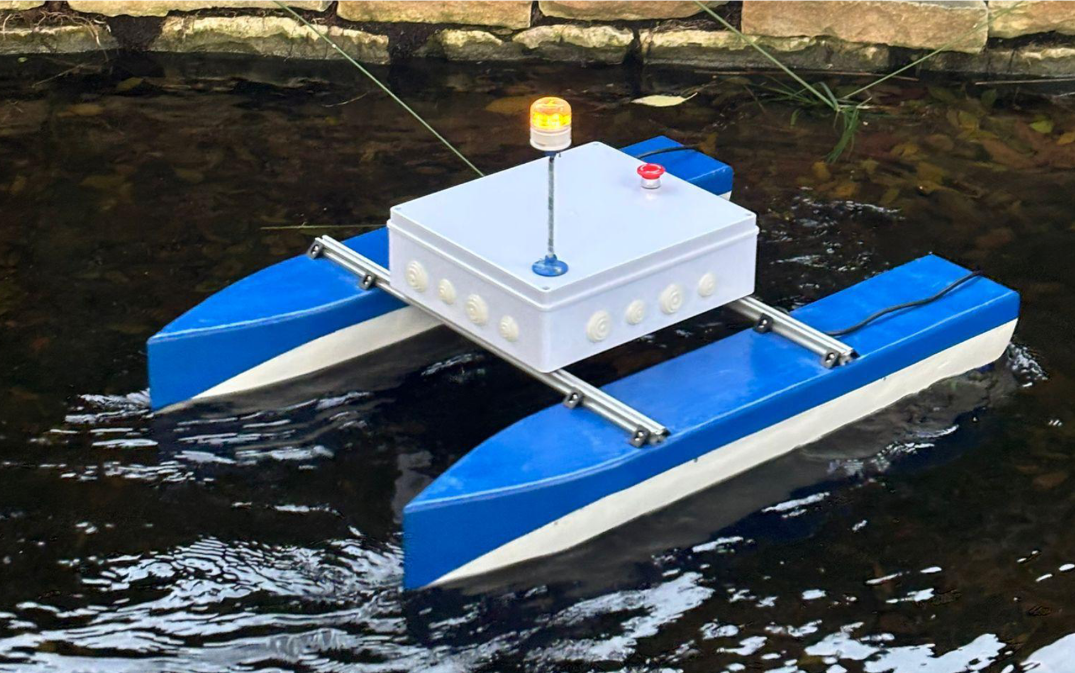
\includegraphics[width=0.5\linewidth]{figuras/usv-francisco.png}
    \caption[Estrutura do \gls{usv}]{Estrutura do \gls{usv} \cite{catamara-telecomandado}}
    \label{fig:usv-francisco}
\end{figure}

Para este processo foi utilizada uma impressora Ender 3 de primeira geração, modificada com a adição de um eixo vertical de 1,5 metros, de forma a possibilitar a produção de peças de maior dimensão. O material escolhido foi PLA, posteriormente reforçado com fibra de vidro, garantindo maior resistência mecânica e durabilidade em ambiente marítimo. 

No centro da estrutura foi instalada uma caixa estanque, destinada a albergar a eletrónica responsável pelo controlo do \gls{usv}, incluindo sensores, interfaces de comunicação e unidades de processamento. Esta caixa integra todos os elementos eletrónicos necessários ao funcionamento do sistema. 

A escolha da estrutura apresentada na Figura \ref{fig:usv-francisco} revela vantagens logísticas significativas. O \gls{usv}-enautica1, embora robusto, apresenta dimensões e peso consideráveis, o que dificulta o seu transporte e limita a sua utilização em testes frequentes. Em contraste, a adoção de um catamarã mais pequeno e leve permite a realização de ensaios de navegação e validação de algoritmos de forma prática e acessível, assegurando maior portabilidade e facilidade de operação.  

É importante salientar que o \gls{usv}-enautica1 utiliza o mesmo tipo de motores \gls{pwm} integrados no protótipo desenvolvido nesta \gls{tfm}, garantindo assim compatibilidade total com os procedimentos de controlo e validação aqui descritos. Esta correspondência tecnológica assegura que os resultados obtidos no protótipo são representativos e transferíveis para sistemas de maior escala.

\section{Motores e Alimentação}
\label{sec:motor}

Tal como o robô didático descrito em \cite{didactic-robot-thesis}, o \gls{usv} desenvolvido neste trabalho recorre a motores para a sua propulsão. No entanto, em vez de motores \gls{dc} utilizados em protótipos educacionais, optou-se pela integração de propulsores subaquáticos de maior robustez, adequados ao ambiente de operação marítima. Estes propulsores, demonstrados na Figura \ref{fig:thrusters}, também conhecidos como \emph{thrusters}, são motores elétricos \emph{brushless} acoplados a hélices, cuja função é gerar empuxo ao movimentar o fluido envolvente (água), permitindo o deslocamento da embarcação.

\begin{figure}[H]
    \centering
    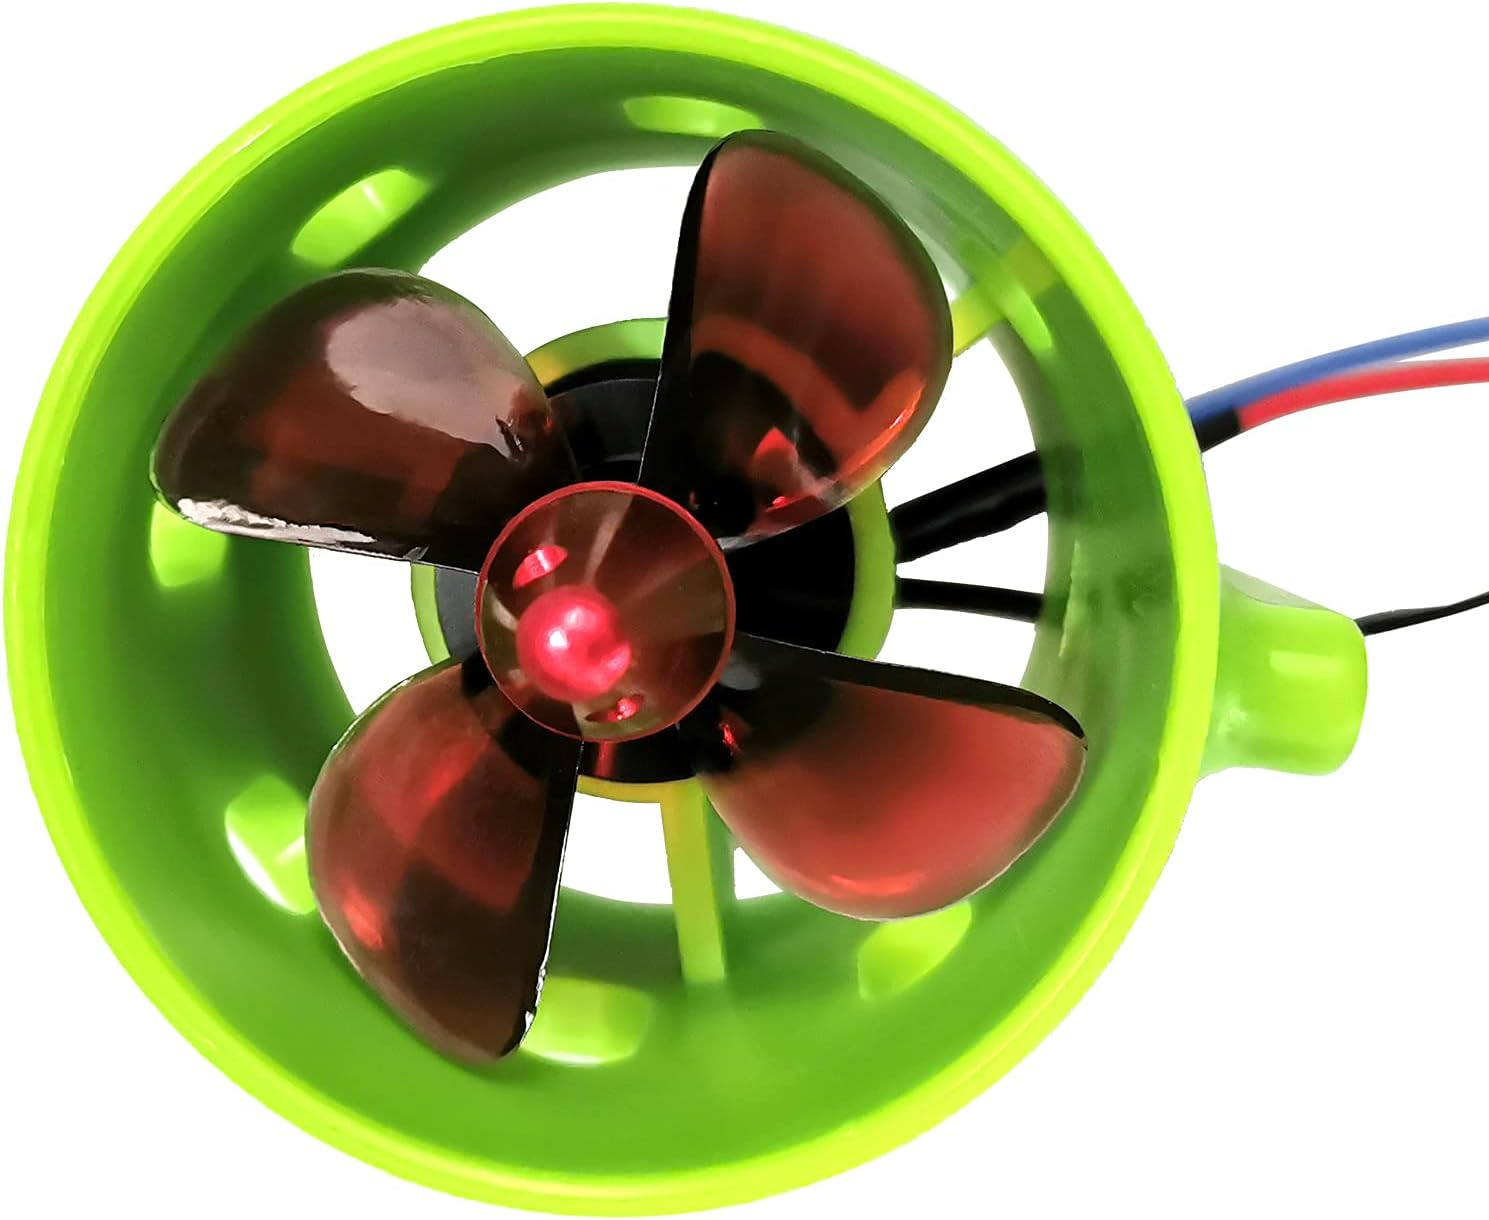
\includegraphics[width=0.33\linewidth]{figuras/thrusters.jpg}
    \caption{Propulsores \emph{brushless} utilizados no \gls{usv}}
    \label{fig:thrusters}
\end{figure}

% empuxo: força de propulsão gerada por um motor/hélice ao mover um fluido
Para este projeto foram selecionados os propulsores U01 \cite{apisqueen-underwater-thruster}, concebidos para aplicações em veículos de superfície e submersíveis de pequena escala. Estes motores operam numa faixa de tensão de 12 a 16 V, com uma potência nominal de 200 W, proporcionando até 2 kgf de empuxo em ambos os sentidos de rotação, uma vez que o seu controlador eletrónico (\gls{esc}) permite controlo bidirecional. Esta característica é essencial para o \gls{usv}, uma vez que garante a manobrabilidade necessária tanto para navegação em linha reta como para rotações em torno do próprio eixo permitindo mudar a direção da embarcação.

Para aplicações que exijam maior potência, podem ser utilizados motores mais robustos, como o Endura C2 \cite{datasheet-endura-c2} presentes no \gls{usv}-enautica1 da Sea2Future \cite{sea2future} \cite{sea2future2} e ilustrados tanto na Figura \ref{fig:sea2future} como na Figura \ref{fig:endura-c2}.

\begin{figure}[H]
    \centering
    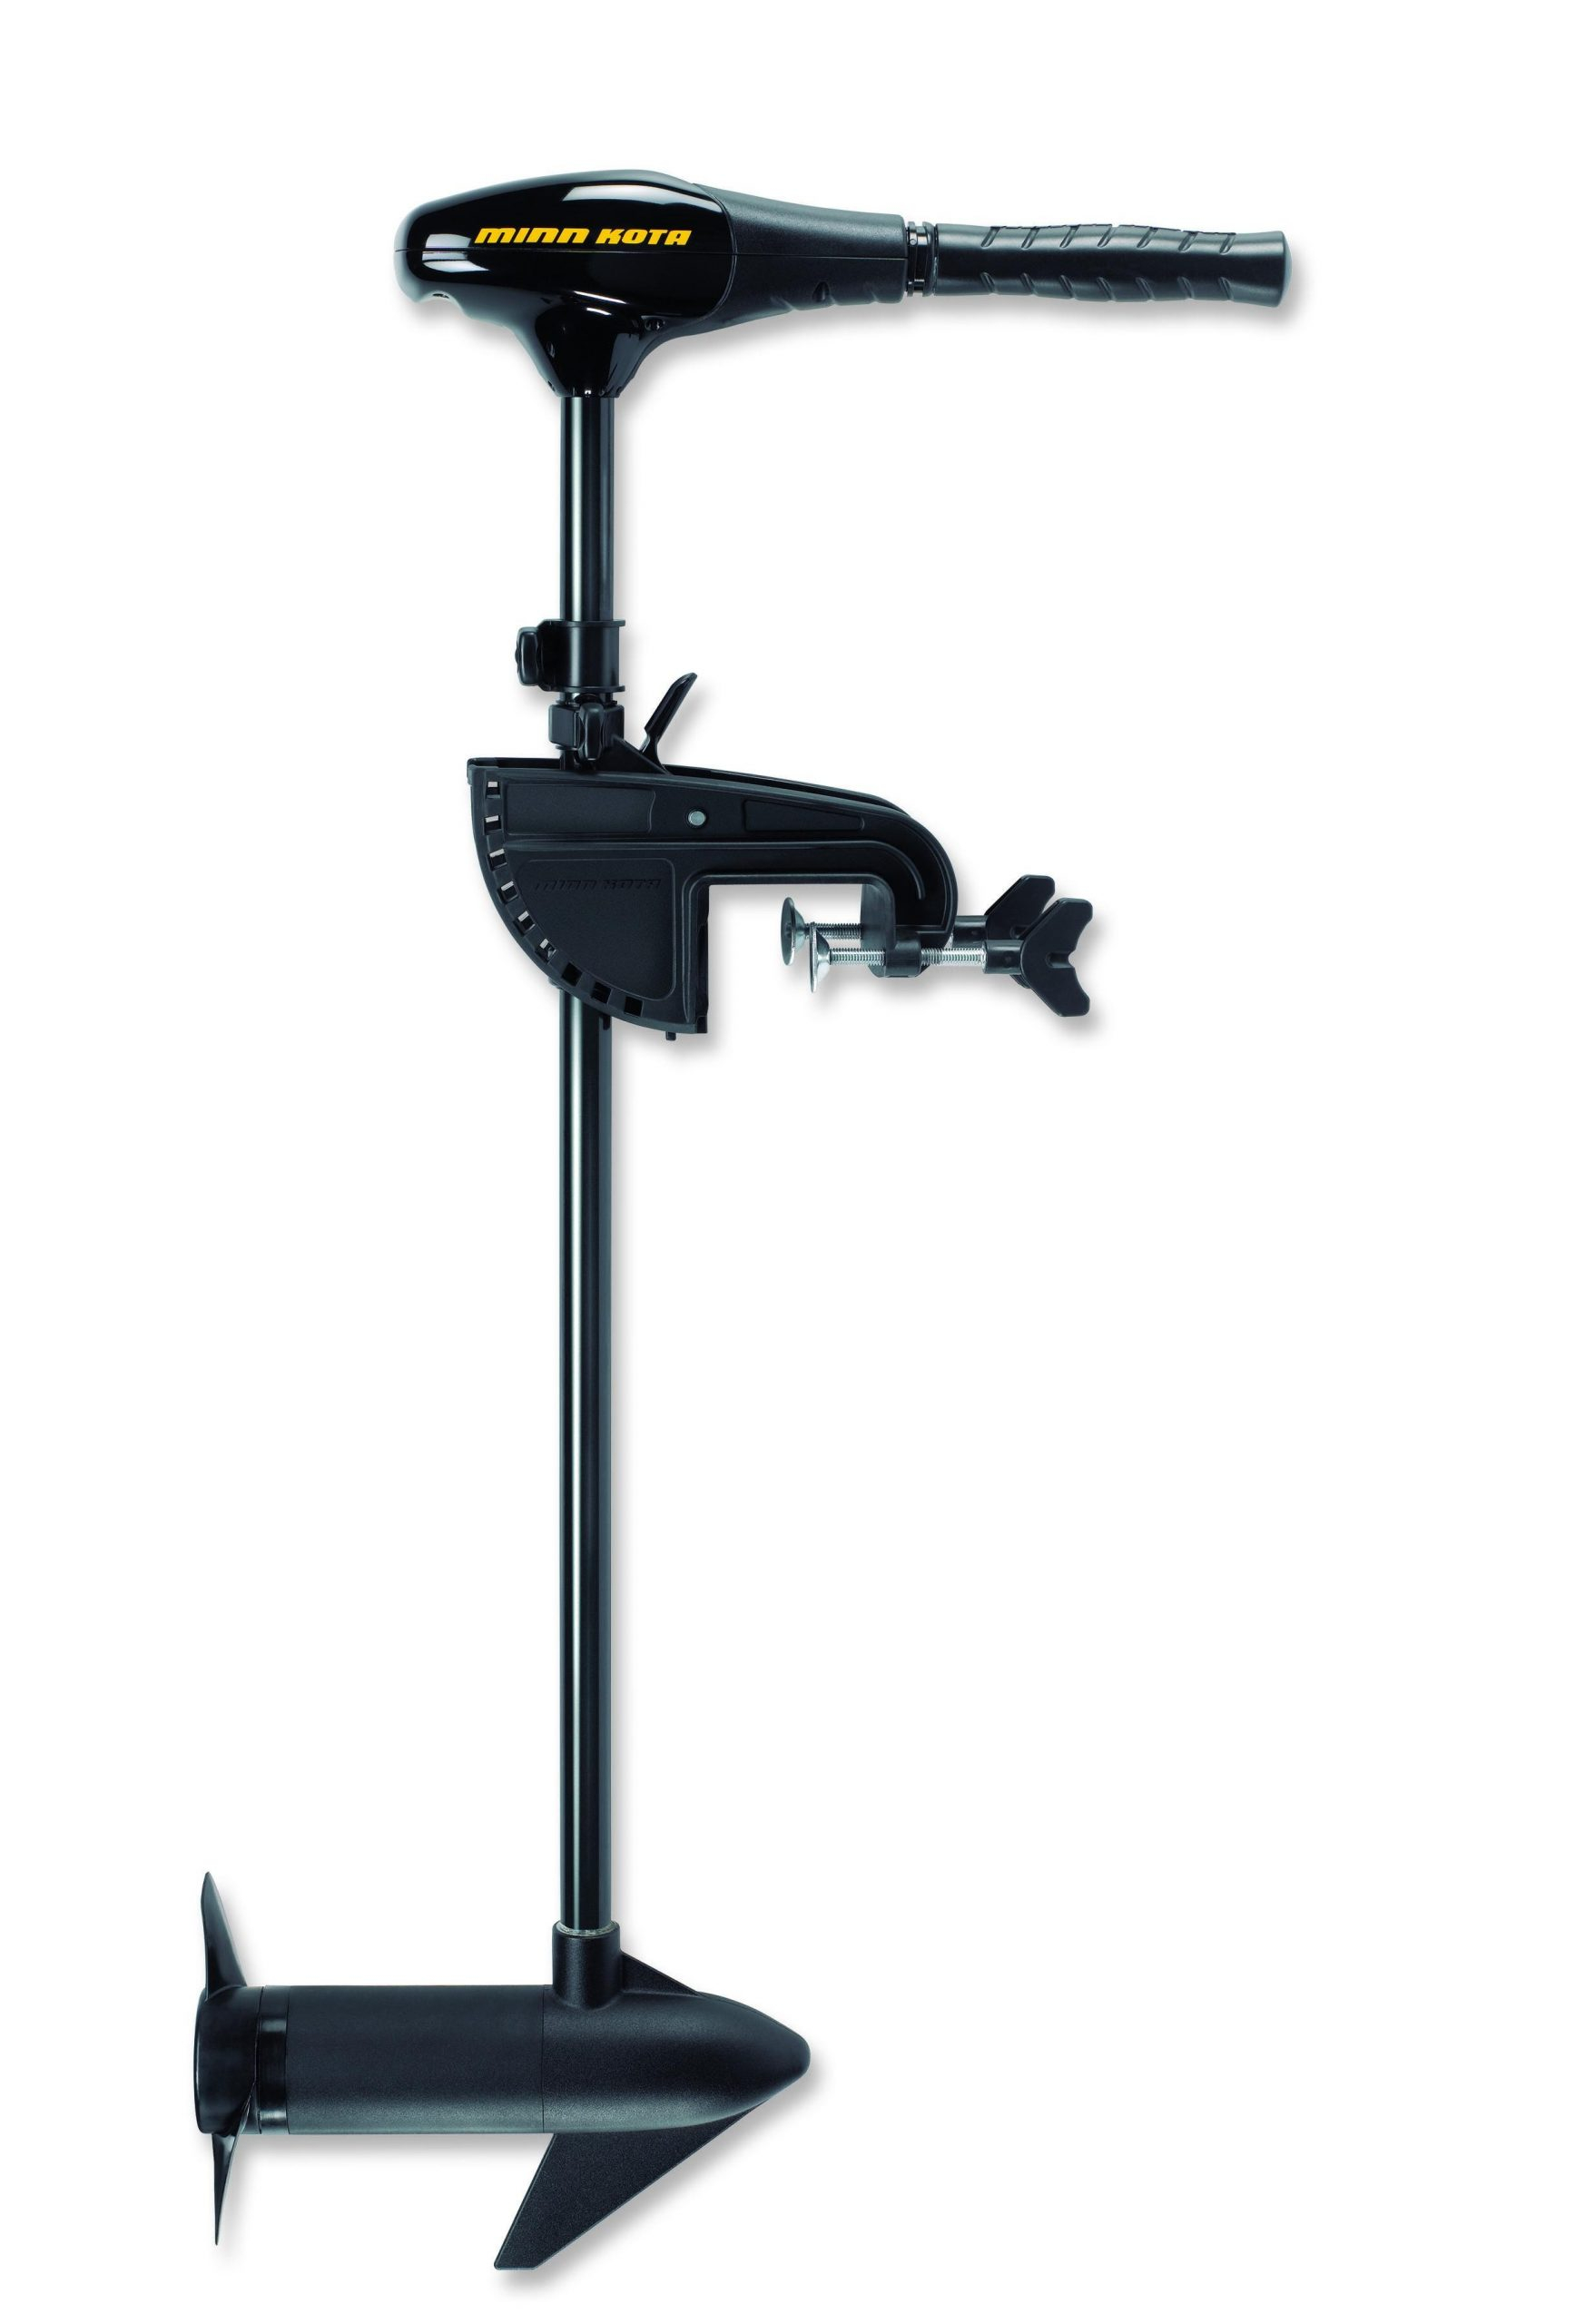
\includegraphics[width=0.33\linewidth]{figuras/endura-c2.jpg}
    \caption[Propulsores Endura C2]{Propulsores Endura C2 \cite{datasheet-endura-c2}}
    \label{fig:endura-c2}
\end{figure}

Os Endura C2 requerem 30A e são também alimentados externamente por uma bateria de 12V.

Em termos de integração elétrica, como ilustrado na Figura \ref{fig:bat-thruster}, cada motor é alimentado por uma bateria de 12 V de elevada capacidade, de forma a suportar a potência exigida e garantir autonomia de operação durante missões prolongadas. A escolha de propulsores \emph{brushless} deve-se a várias vantagens face aos motores \gls{dc} convencionais: maior eficiência energética, menor desgaste mecânico devido à ausência de escovas, capacidade de fornecer binário elevado a baixas rotações e maior fiabilidade em condições ambientais adversas, como a exposição contínua à água.

Adicionalmente, o sistema de controlo utiliza sinais de \gls{pwm} gerados pelo microcontrolador principal, que são interpretados pelo \gls{esc} de cada motor. Este mecanismo permite ajustar de forma contínua a velocidade e o sentido de rotação, possibilitando manobras precisas, tais como mudanças bruscas de direção ou movimentos de baixa velocidade em ambientes restritos.

A adoção de dois propulsores oferece um equilíbrio entre simplicidade e manobrabilidade, permitindo que o \gls{usv} execute translações e rotações sem necessidade de sistemas de direção adicionais. Contudo, a arquitetura do sistema foi concebida para ser escalável, suportando até quatro propulsores, caso seja necessário aumentar a estabilidade, a potência de propulsão ou a capacidade de operação em cenários marítimos mais exigentes.

\begin{figure}[H]
    \centering
    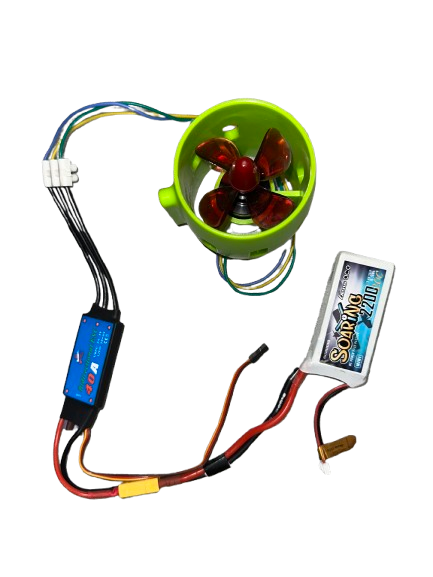
\includegraphics[width=0.5\linewidth, angle=-90]{figuras/IMG_4420-removebg-preview.png}
    \caption{Integração elétrica dos propulsores}
    \label{fig:bat-thruster}
\end{figure}

\section{\acrfull{esc}}
\label{sec:esc}

O \acrfull{esc} é o componente responsável por controlar o funcionamento dos motores \emph{brushless} utilizados no \gls{usv}. Este dispositivo converte o sinal de comando proveniente do microcontrolador em impulsos elétricos adequados para alimentar as bobinas do motor, garantindo a regulação da sua velocidade e direção de rotação.

A Figura \ref{fig:pwm-sinal} apresenta a forma de onda do sinal de \gls{pwm} aplicado ao \gls{esc} para controlar os \emph{thursters}.implementação. A Figura 4.3 apresenta a forma de onda do sinal de \gls{pwm} descrito.

O princípio de funcionamento baseia-se na utilização de sinais de \gls{pwm} enviados pelo microcontrolador. Estes sinais consistem em pulsos periódicos cuja largura (duração em microssegundos) determina a resposta do motor \cite{didactic-robot-thesis}. Tipicamente, um sinal com largura de $1000\,\mu s$ (linha azul da Figura \ref{fig:pwm-sinal}) corresponde à velocidade mínima no sentido inverso, $1500\,\mu s$ (linha laranja da Figura \ref{fig:pwm-sinal}) corresponde ao ponto neutro, no qual o motor permanece parado, e $2000\,\mu s$ (linha verde da Figura \ref{fig:pwm-sinal}) corresponde à velocidade máxima no sentido direto. A partir deste ponto central, a largura do pulso varia de forma simétrica: valores inferiores a $1500\,\mu s$ comandam rotações no sentido inverso com velocidade crescente à medida que a largura do pulso diminui, enquanto valores superiores a $1500\,\mu s$ comandam rotações no sentido direto com velocidade crescente à medida que a largura do pulso aumenta. A frequência habitual do sinal é de $50\,Hz$, o que significa que cada período tem $20000\,\mu s$. Este padrão segue a mesma lógica dos sinais de controlo usados em servomotores, o que facilita a sua implementação e utilização de controladores \emph{standard} de radio controle utilizado em modelismo. 

\begin{figure}[H]
    \centering
    % Substituir pelo diagrama do sinal PWM (1000 \(\mu s\), 1500 \(\mu s\), 2000 \(\mu s\))
    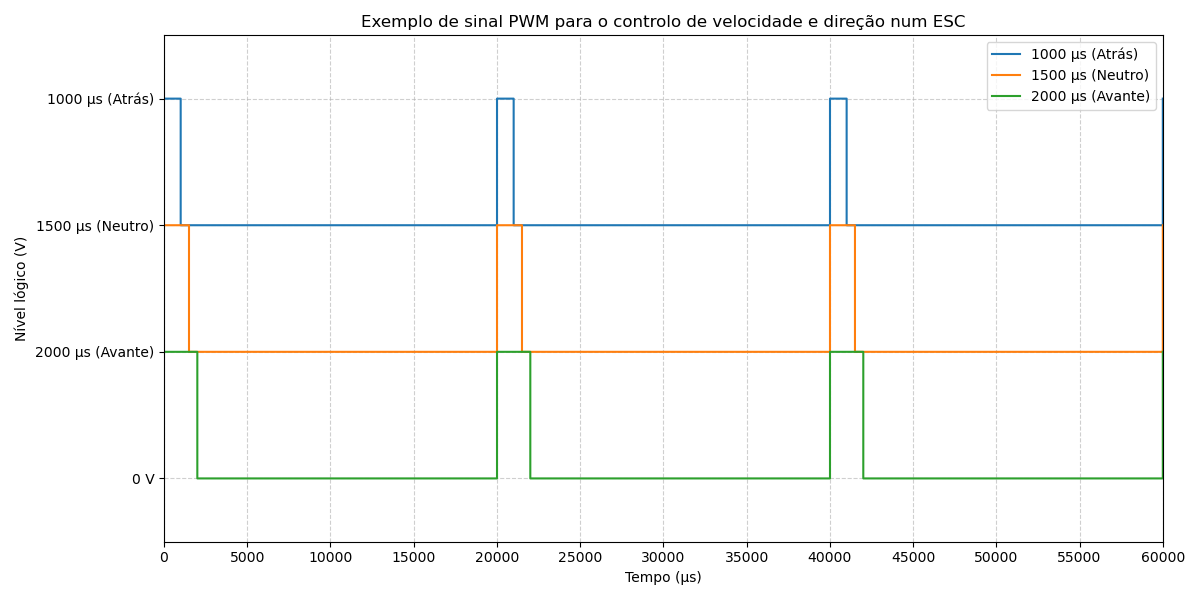
\includegraphics[width=1\linewidth]{figuras/pwm_us.png}
    \caption{Exemplo de sinal \gls{pwm} para o controlo de velocidade e direção num \gls{esc}}
    \label{fig:pwm-sinal}
\end{figure}

Antes de os motores poderem ser utilizados, o \gls{esc} necessita de ser armado, este processo consiste na aplicação de uma sequência de sinais de inicialização que confirmam a ligação entre o controlador e o motor, garantindo que este não entra em funcionamento acidentalmente. No caso em estudo, este procedimento envolve enviar inicialmente um sinal de largura mínima (por exemplo, $1000\,\mu s$) durante 2 segundos, seguido da transição para a largura correspondente ao ponto neutro ($1500\,\mu s$). Apenas após esta sequência o \gls{esc} considera o sistema pronto a operar, emitindo normalmente sinais sonoros característicos que confirmam o estado de prontidão.

O controlo bidirecional da rotação é assegurado pelo próprio \gls{esc}, que interpreta os sinais de \gls{pwm} acima e abaixo do ponto neutro. Assim:

\begin{itemize}
    \item Pulsos inferiores a $1500\,\mu s$ comandam a rotação no sentido inverso (atrás);
    \item Pulsos superiores a $1500\,\mu s$ comandam a rotação no sentido direto (avante).
\end{itemize}

Este mecanismo elimina a necessidade de sistemas mecânicos de inversão de polaridade, uma vez que o \gls{esc} efetua digitalmente a comutação das fases do motor \emph{brushless}. A grande vantagem desta abordagem é a elevada precisão no controlo da velocidade, associada a uma resposta rápida e eficiente, fatores críticos para a manobrabilidade do \gls{usv} em cenários marítimos complexos.

Em síntese, o \gls{esc} desempenha um papel central no sistema de propulsão: traduz os comandos enviados pelo microcontrolador em potência controlada para os motores, garante a segurança durante a inicialização através do processo de armamento, e possibilita a rotação bidirecional através da modulação do sinal \gls{pwm}.

\section{Sensores} 
\label{sec:sensores}

A operação autónoma de um \gls{usv} depende fortemente da disponibilidade de sensores capazes de fornecer medições fiáveis sobre a sua posição, movimento e orientação. Estes dados constituem a base para o controlo de navegação, permitindo não apenas o seguimento rigoroso de rotas previamente definidas, mas também a correção dinâmica de desvios causados por correntes, ondas ou vento.  

No protótipo desenvolvido, a arquitetura de sensorização foi concebida de forma modular, possibilitando a integração e substituição de sensores de maneira independente, sem comprometer a funcionalidade global. Esta abordagem garante escalabilidade e flexibilidade, permitindo adaptar o sistema a diferentes cenários operacionais ou evoluir para missões com requisitos mais complexos.  

Entre os sensores integrados, destacam-se dois elementos centrais. O primeiro é a \acrfull{imu}, responsável por medir aceleração, velocidade angular e intensidade do campo magnético, permitindo calcular com elevada precisão a orientação do veículo nos três eixos principais (\emph{yaw}, \emph{pitch} e \emph{roll}). O segundo é o recetor \acrfull{gps}, que fornece a posição geográfica absoluta em coordenadas de latitude e longitude, constituindo a referência essencial para a definição e seguimento de \emph{waypoints}.  

O uso combinado destes dois sensores permite mitigar as limitações individuais de cada um: enquanto o \gls{imu} fornece dados de orientação com elevada taxa de atualização, mas sofre de erro acumulado, o \gls{gps} disponibiliza medições absolutas de posição, embora com menor frequência e suscetíveis a erros momentâneos. Assim, a fusão de dados provenientes de ambos os sensores garante maior precisão, robustez e fiabilidade na estimativa da trajetória do \gls{usv}.  

As subseções seguintes apresentam em detalhe a integração da \acrfull{imu} (Subsecção \ref{subsec:imu}) e do recetor \acrfull{gps} (Subsecção \ref{subsec:gps}), descrevendo os princípios de funcionamento, a configuração adotada e o contributo de cada sensor para a arquitetura global de navegação.


\subsection{\acrfull{imu}} \label{subsec:imu}

O \gls{imu} é um dispositivo essencial para medir a orientação e o movimento do \gls{usv}. Este sensor combina acelerómetros, giroscópios e, em alguns casos, magnetómetros, fornecendo dados sobre aceleração linear, taxas de rotação e direção magnética. Estas medições são processadas para determinar os ângulos de guinada (\emph{yaw}), arfagem (\emph{pitch}) e rotação (\emph{roll}), que descrevem a orientação do veículo no espaço tridimensional, tal como ilustrado na Figura \ref{fig:pitch-roll-yaw}.

\begin{figure}[H]
    \centering
    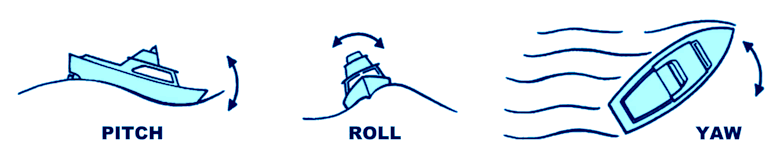
\includegraphics[height=0.2\linewidth]{figuras/Pitch-Roll-Yaw.png}
    \caption[Representação do \emph{yaw}, \emph{pitch} e \emph{roll} numa embarcação]{Representação do \emph{yaw}, \emph{pitch} e \emph{roll} numa embarcação \cite{imagem-yaw-pitch-roll}}
    \label{fig:pitch-roll-yaw}
\end{figure}

O \emph{yaw} representa a rotação em torno do eixo vertical e é essencial para controlar a direção do \gls{usv}. O \emph{pitch} mede a inclinação em torno do eixo horizontal, sendo crítico para avaliar o impacto de ondas e alterações na estabilidade longitudinal. Já o \emph{roll} refere-se à oscilação lateral em torno do eixo longitudinal, desempenhando um papel importante na manutenção da estabilidade transversal da embarcação.

Para este projeto, foram avaliadas diversas opções de \gls{imu} culminando em duas opções: o MPU6050 e o MPU9250. O MPU6050 é um sensor de 6 eixos que integra um acelerómetro e um giroscópio, permitindo medições básicas de orientação e movimento. Apesar da sua simplicidade e baixo custo, a ausência de um magnetómetro limita a sua capacidade de fornecer orientação absoluta, o que pode ser um fator crítico em qualquer aplicação que necessite dos conceitos anteriormente descritos. Por outro lado, o MPU9250 é um sensor de 9 eixos que, além do acelerómetro e do giroscópio, inclui um magnetómetro. Este último componente possibilita medições do campo magnético terrestre, fornecendo informações sobre a direção absoluta, algo indispensável para sistemas de navegação autónoma que dependem de dados precisos para evitar desvios ou erros acumulados.

A escolha do MPU9250 (ou equivalente) foi motivada pela sua superioridade técnica em comparação com o MPU6050. A inclusão de um magnetómetro permite compensar erros acumulados pelo giroscópio, garantindo medições mais estáveis e precisas em condições dinâmicas. Além disso, o suporte a técnicas de fusão de sensores (\emph{sensor fusion}), que combinam dados do acelerómetro, giroscópio e magnetómetro, aumenta significativamente a fiabilidade das estimativas de orientação. Apesar de o MPU9250 ter um custo ligeiramente superior e exigir maior esforço de calibração, as suas vantagens, como a capacidade de medição absoluta de orientação, justificam plenamente a sua integração no sistema.

Com o MPU9250, o sistema é capaz de calcular e ajustar a orientação do \gls{usv} em tempo real, permitindo a correção de rota em resposta a forças externas, como correntes marítimas e ondas. Para contextualizar melhor este processo, apresentam-se de seguida os conceitos fundamentais de \emph{yaw}, \emph{pitch} e \emph{roll}, que descrevem a orientação da embarcação nos três eixos principais.

\subsubsection{\emph{Yaw} (\(\Psi\))}
O ângulo de Yaw (\(\Psi\)) representa a rotação em torno do eixo vertical (\(z\)) (Figura \ref{fig:yaw}) e é calculado utilizando os dados do magnetómetro, corrigidos pela inclinação com base nos ângulos de \emph{pitch} e \emph{roll}. 

\begin{figure}[H]
    \centering
    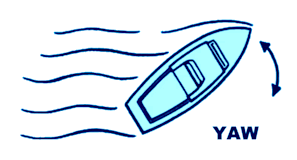
\includegraphics[height=0.2\linewidth]{figuras/Yaw.png}
    \caption[Representação do yaw numa embarcação]{Representação do yaw numa embarcação (Adaptada de \cite{imagem-yaw-pitch-roll})}
    \label{fig:yaw}
\end{figure}

Primeiramente, calcula-se \(m_x'\) utilizando a Equação \ref{eq:mx_prime}.

\begin{equation}
    m_x' = m_x \cos(\Theta) + m_z \sin(\Theta)
    \label{eq:mx_prime}
    % \lstequation{Cálculo de \(m_x'\)}
\end{equation}

Em seguida, \(m_y'\) é obtido com base na Equação \ref{eq:my_prime}.

\begin{equation}
    m_y' = m_x \sin(\Phi) \sin(\Theta) + m_y \cos(\Phi) - m_z \sin(\Phi) \cos(\Theta)
    \label{eq:my_prime}
    % \lstequation{Cálculo de \(m_y'\)}
\end{equation}

Finalmente, o ângulo de \emph{yaw} (\(\Psi\)) é determinado através da Equação \ref{eq:yaw}. 

\begin{equation}
    \Psi = \arctan2(-m_y', m_x')
    \label{eq:yaw}
    % \lstequation{Cálculo do ângulo de Yaw (\(\Psi\))}
\end{equation}

Aqui, \(m_x\), \(m_y\) e \(m_z\) são as medições do magnetómetro nos eixos \(x\), \(y\) e \(z\), respetivamente, e os ângulos \(\Theta\) (pitch) e \(\Phi\) (roll) corrigem a inclinação do sensor.

\subsubsection{\emph{Pitch} (\(\Theta\))}
O ângulo de  \emph{pitch} (\(\Theta\)) representa a inclinação do sensor para frente e para trás (Figura \ref{fig:pitch}).

\begin{figure}[H]
    \centering
    
\includegraphics[height=0.2\linewidth]{figuras/Pitch.png}
    \caption[Representação do \emph{pitch} numa embarcação]{Representação do \emph{pitch} numa embarcação (Adaptada de \cite{imagem-yaw-pitch-roll})}
    \label{fig:pitch}
\end{figure}

Sendo calculado diretamente com base nas medições do acelerómetro, conforme a Equação \ref{eq:pitch}.

\begin{equation}
    \Theta = \arcsin{\left(\frac{-a_x}{\sqrt{a_x^2 + a_y^2 + a_z^2}}\right)}
    \label{eq:pitch}
\end{equation}

onde \(a_x\), \(a_y\) e \(a_z\) correspondem às acelerações medidas nos eixos \(x\), \(y\) e \(z\), respetivamente.

\subsubsection{\emph{Roll} (\(\Phi\))}
O ângulo de \emph{roll} (\(\Phi\)) representa a inclinação lateral (esquerda/direita) (Figura \ref{fig:roll}) e é derivado das medições do acelerómetro, como descrito na Equação \ref{eq:roll}.

\begin{figure}[H]
    \centering
    
\includegraphics[height=0.2\linewidth]{figuras/Roll.png}
    \caption[Representação do \emph{roll} numa embarcação]{Representação do \emph{roll} numa embarcação (Adaptada de \cite{imagem-yaw-pitch-roll})}
    \label{fig:roll}
\end{figure}

\begin{equation}
    \Phi = \arctan2{\left(a_y, a_z\right)}
    \label{eq:roll}
    % \lstequation{Cálculo do ângulo de Roll (\(\Phi\))}
\end{equation}

onde \(a_y\) e \(a_z\) são as acelerações medidas nos eixos \(y\) e \(z\), respetivamente. A função \(\arctan2\) é usada para garantir que o ângulo esteja no quadrante correto.

\subsection{\acrfull{gps}} \label{subsec:gps}

O \gls{gps} é uma tecnologia amplamente utilizada para a determinação da posição geográfica de objetos ou indivíduos em qualquer ponto do globo. Este sistema, desenvolvido inicialmente pelo Departamento de Defesa dos Estados Unidos, é constituído por uma constelação de satélites que transmitem sinais de rádio para dispositivos recetores na Terra. Estes sinais são processados para calcular coordenadas geográficas com elevada precisão, fornecendo informações cruciais em aplicações de navegação, monitorização e controlo de sistemas móveis, como veículos autónomos.

O funcionamento do \gls{gps} baseia-se no princípio da triangulação, tal como se pode observar na Figura \ref{fig:triangulacao}), onde pelo menos quatro satélites são necessários para determinar com precisão a posição de um recetor no espaço tridimensional (latitude, longitude e altitude). Cada satélite transmite sinais codificados contendo informações sobre a sua posição e o tempo exato em que o sinal foi enviado. O recetor \gls{gps} calcula o tempo que o sinal levou a chegar a partir de múltiplos satélites, determinando assim a distância de cada um. Com base nestes dados, a posição do recetor é triangulada. 

No caso do \gls{usv}, apenas são necessários três satélites, pois não é necessário determinar a altitude. Como o \gls{usv} opera na superfície da água, a sua posição é restrita a um plano bidimensional, considerando apenas latitude e longitude. Desta forma, a triangulação pode ser realizada com precisão utilizando apenas três satélites, simplificando o cálculo em relação a sistemas que requerem coordenadas tridimensionais.

\begin{figure}[H]
    \centering
    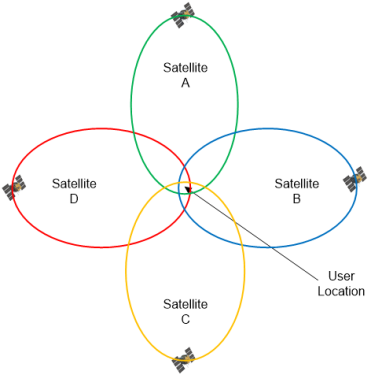
\includegraphics[width=0.33\linewidth]{figuras/lowdop.png}
    \caption[Triangulação do sinal \gls{gps}]{Triangulação do sinal \gls{gps} \cite{help-gps}}
    \label{fig:triangulacao}
\end{figure}

O sistema \gls{gps} depende de relógios atómicos precisos instalados nos satélites para garantir a sincronização temporal. Além disso, algoritmos avançados compensam erros causados por fatores como a atmosfera terrestre e o desvio orbital dos satélites.

Entre as principais vantagens do \gls{gps}, destacam-se a sua elevada precisão, que em condições ideais permite obter localizações com margens de erro de poucos metros, e a cobertura global, que garante funcionalidade em qualquer lugar do mundo, independentemente de fronteiras geográficas. Adicionalmente, o recetor \gls{gps} opera de forma passiva, recebendo sinais sem necessidade de os transmitir, o que contribui para a eficiência energética. A sua facilidade de integração em sistemas autónomos, como os \gls{usv} descritos nesta \gls{tfm}, é também uma característica relevante.

Por outro lado, o \gls{gps} apresenta algumas limitações, como a dependência de visibilidade direta com os satélites, sendo o sinal frequentemente bloqueado por obstáculos como edifícios, montanhas, vegetação ou nuvêns densas. As condições atmosféricas, incluindo tempestades solares e interferências atmosféricas, podem comprometer a precisão do sistema. Além disso, o consumo energético do recetor, embora moderado, pode ser um desafio em dispositivos com baterias de capacidade limitada. Por fim, o \gls{gps} é vulnerável a interferências e bloqueios intencionais (\emph{jamming}), o que reduz a sua fiabilidade em situações críticas.

Apesar da possibilidade de utilizar apenas um \gls{imu} para estimar a posição e orientação do \gls{usv}, esta abordagem revela-se insuficiente em aplicações que exigem elevada precisão em trajetos extensos. O \gls{imu} utiliza sensores como acelerómetros e giroscópios para calcular deslocações relativas, mas está sujeito a deriva acumulada ao longo do tempo devido a erros nos sensores e no processamento de dados. A combinação com um \gls{gps} é, portanto, fundamental, uma vez que este fornece medições absolutas que corrigem a deriva inerente ao \gls{imu}, assegurando uma navegação fiável e precisa.  

Importa salientar que recetores \gls{gps} são tipicamente configurados e utilizados através de portas série (\gls{uart}), o que representa um desafio quando se pretende integrar múltiplos módulos num sistema que privilegia a comunicação via \gls{i2c}. No contexto desta \gls{tfm}, foi definido como requisito que todos os módulos comunicassem preferencialmente através do barramento \gls{i2c}, de modo a simplificar a arquitetura e reduzir o número de interfaces independentes no microcontrolador. Para alcançar este objetivo, foi integrado um conversor \gls{i2c}-\gls{uart} (SC16IS750), que atua como uma ponte entre os dois protocolos. Esta solução permitiu expandir o número de interfaces série disponíveis sem comprometer a modularidade da arquitetura, garantindo a integração eficiente do \gls{gps} e mantendo a uniformidade da comunicação entre os diferentes módulos do sistema.  

Concluída a descrição dos sensores principais, torna-se agora pertinente apresentar as interfaces de comunicação adotadas no sistema, que asseguram não apenas a ligação entre sensores e atuadores, mas também a transmissão de dados com a estação remota. Entre estas destacam-se a comunicação de longo alcance via \gls{lora}, o barramento \gls{i2c} como espinha dorsal do sistema modular, e a utilização pontual do \gls{uart} para integração de dispositivos específicos.

\section{Interfaces de Comunicação}

Nesta secção são apresentadas as principais interfaces de comunicação utilizadas no desenvolvimento do sistema, fundamentais para assegurar a integração entre sensores, atuadores e a estação remota. A escolha das tecnologias de comunicação teve em consideração critérios de alcance, eficiência energética, simplicidade de implementação e escalabilidade da arquitetura. São analisadas três interfaces complementares: i) o \gls{lora}, responsável pela comunicação de longo alcance e pela transmissão de telemetria em tempo real; ii) o \gls{i2c}, que constitui o barramento principal para a integração modular de sensores e controladores; e iii) o \gls{uart}, utilizado em casos específicos, como na ligação de recetores \gls{gps}, através de conversores dedicados.  

\subsection{\acrfull{lora}}

No contexto de sistemas ciber-físicos e veículos autónomos, a seleção da interface de comunicação é um elemento essencial para garantir a troca eficiente e confiável de dados entre os diferentes módulos do sistema. As interfaces de comunicação desempenham um papel fundamental na transmissão de telemetria, atualizações de rota e integração de sensores em tempo real. Neste projeto, foi escolhido o uso de \gls{lora} como tecnologia principal, devido às suas características únicas, especialmente em aplicações que requerem comunicações de longa distância com baixo consumo energético.

O \gls{lora} é uma tecnologia de comunicação sem fios desenvolvida especificamente para sistemas de longa distância e baixo consumo de energia. Utilizando a modulação de espalhamento espectral (\emph{chirp spread spectrum}), o \gls{lora} é capaz de transmitir dados a distâncias que podem ultrapassar 10 km em linha de vista, enquanto consome uma fração da energia necessária para tecnologias de maior largura de banda, como LTE \cite{wikipedia-lte} ou 4G \cite{wikipedia-4g,bivocom-lte-vs-lora}.  

Comparado com outras tecnologias, como LTE/4G e XBee \cite{digi-xbee}, o \gls{lora} apresenta vantagens específicas para sistemas remotos e energeticamente eficientes. O LTE/4G oferece velocidades de transmissão muito superiores, sendo ideal para aplicações que exigem elevada largura de banda, como \textit{streaming} de vídeo ou comunicação em tempo real. No entanto, o seu elevado consumo energético e dependência de infraestrutura de telecomunicações tornam-no inadequado para dispositivos móveis em áreas remotas \cite{bivocom-lte-vs-lora}. Já o XBee, uma solução de curto alcance baseada em Zigbee, destaca-se pela simplicidade de integração e baixo consumo energético, mas a sua limitada cobertura geográfica restringe significativamente o seu uso em comunicações de longa distância \cite{digi-xbee-specs, xbee-range-comparison}. Assim, o \gls{lora} apresenta-se como uma alternativa equilibrada, unindo alcance estendido e eficiência energética, especialmente relevante para este projeto.

Entre as vantagens do \gls{lora}, destacam-se o alcance de comunicação longo, que pode superar 10 km em condições ideais, e o baixo consumo energético, essencial para prolongar a autonomia de dispositivos alimentados por bateria. A modulação utilizada oferece robustez contra interferências e ruídos, garantindo comunicação confiável em ambientes adversos, e o custo de implementação, tanto em termos de \emph{hardware} como de infraestrutura, é significativamente inferior ao de outras soluções como LTE/4G. Por outro lado, o \gls{lora} também possui limitações, como a baixa largura de banda, que o torna inadequado para transmissão de grandes volumes de dados, e uma maior latência na entrega de mensagens, que pode ser problemática para aplicações que exigem respostas em tempo real. Adicionalmente, a infraestrutura de comunicação pode necessitar de gateways específicos para integração com redes de maior escala, o que pode ser um desafio em cenários de maior complexidade.

Em termos de alcance, a tecnologia \gls{lora} tem demonstrado um grande potencial (cerca de 45 vezes o alcance inicialmente proposto pela empresa Semtech, a criadora do \gls{lora}). Recentemente, em Portugal, foi estabelecido um novo recorde de distância com \gls{lora}, atingindo os 1336 km \cite{pplware-lora}. Este feito foi realizado no âmbito do projeto Custodian, com a instalação de trackers \gls{lora} num barco de pesca e nas suas boias na costa de Sesimbra, Portugal. O tracker estabeleceu comunicação com um portal nas Ilhas Canárias, localizando-se a mais de 1.300 km de distância. Este recorde foi alcançado ao nível do mar, o que elimina variáveis potenciais introduzidas por altitudes variadas e fornece uma medida mais padronizada das capacidades da tecnologia. Este marco é particularmente notável, pois demonstra a robustez da tecnologia \gls{lora} para comunicações de longa distância em condições reais, e sublinha a sua capacidade de ultrapassar distâncias que antes eram consideradas inatingíveis para outras tecnologias de comunicação sem fios.

A Tabela \ref{tab:comparacao_comunicacao} apresenta as diferenças de desempenho entre as tecnologias de comunicação avaliadas para este projeto.

\begin{table}[H]
    \centering
    \caption{Comparação entre Tecnologias de Comunicação}
    \label{tab:comparacao_comunicacao}
    \begin{tabular}{lccc}
        \textbf{Tecnologia} & \textbf{Alcance (m)} & \textbf{Consumo Energético (mW)} & \textbf{Largura de Banda (kbps)} \\ \hline 
        \gls{lora} & Até 1 336 & 10--50 & 0.3--50 \\ 
        LTE/4G & Até 20 000 & 1 000--2 000 & 1 000--100 000 \\ 
        XBee (Zigbee) & Até 100 & 40--60 & 20--250 \\
        \hline 
    \end{tabular}%
\end{table}

O \gls{lora} foi escolhido devido ao seu baixo consumo energético, crucial para otimizar a autonomia em sistemas ciber-físicos alimentados por bateria, e ao seu longo alcance, que garante comunicações robustas em ambientes remotos sem a necessidade de infraestrutura complexa. A escolha do \gls{lora} como interface de comunicação foi uma decisão estratégica, uma vez que permite a transmissão de dados de telemetria e a atualização de rotas em locais onde tecnologias como LTE/4G ou XBee seriam inviáveis, seja por questões práticas ou económicas. Assim, a aplicação do \gls{lora} neste sistema ciber-físico assegura o cumprimento dos objetivos de eficiência energética e robustez operacional, oferecendo uma solução confiável e alinhada com os desafios reais enfrentados por \gls{usv}.

\subsection{\acrfull{i2c}} \label{subsec:i2c}

O protocolo \gls{i2c} é um dos mais comuns para comunicação entre dispositivos periféricos em sistemas embebidos, como o \gls{usv}. A sua principal vantagem reside na capacidade de utilizar apenas dois fios para comunicação: um para o relógio (\(SCL\)) e outro para dados (\(SDA\)), o que reduz significativamente a complexidade e o número de conexões no sistema. Este protocolo permite a comunicação entre múltiplos dispositivos com um único controlador mestre e vários escravos, sendo cada dispositivo identificado por um endereço único. Comparado com tecnologias como o \gls{spi}, o \gls{i2c} apresenta uma largura de banda menor e é adequado para distâncias mais curtas.

A utilização do \gls{i2c} neste projeto é fundamental para a integração de sensores e módulos que requerem comunicação de dados de forma eficiente e com baixo consumo energético. A flexibilidade do \gls{i2c} permite expandir facilmente o número de dispositivos conectados ao sistema, com a adição de novos expansores de I/O, como descrito em \cite{didactic-robot-thesis} Secção 4.4, que podem ser utilizados para controlar sensores adicionais ou atuadores, como motores e atuadores de direção. O protocolo \gls{i2c} é amplamente utilizado em módulos de sensores como o MPU9250 (\gls{imu}), que requerem comunicação constante para garantir medições em tempo real da orientação e movimento do \gls{usv}.

Apesar das suas vantagens, o \gls{i2c} apresenta algumas limitações que devem ser consideradas no desenho do sistema. Em primeiro lugar, trata-se de um protocolo \textit{half-duplex}, dado que a linha de dados (SDA) é partilhada para envio e receção, impossibilitando transmissões simultâneas bidirecionais. Além disso, a especificação original suporta até 127 dispositivos endereçáveis, mas na prática este número é frequentemente inferior devido a restrições elétricas e à possibilidade de colisões de endereços entre diferentes módulos. Outro aspeto limitador é o alcance físico do barramento, que tipicamente não deve exceder alguns metros devido à capacitância das linhas, tornando o \gls{i2c} adequado apenas para sistemas compactos. Finalmente, a sua taxa de transferência, que pode variar entre 100 kbit/s (modo standard) e 3,4 Mbit/s (modo \emph{high speed}), é consideravelmente inferior à de protocolos como \gls{spi}, o que pode ser uma limitação em sistemas que requerem alta largura de banda.

\subsection{\acrfull{uart}} 
\label{subsec:uart}

O protocolo \gls{uart} é um dos métodos mais simples e amplamente utilizados para comunicação série em sistemas embebidos. Diferente do \gls{i2c}, em que um dos fios é dedicado ao sinal de relógio (\(SCL\)) e o outro transporta os dados (\(SDA\)), o \gls{uart} utiliza duas linhas independentes: uma para transmissão (\(TX\)) e outra para receção (\(RX\)). Esta característica elimina a necessidade de um sinal de relógio externo e permite que a comunicação seja assíncrona. Para que dois dispositivos comuniquem corretamente, é necessário que concordem previamente sobre parâmetros como a taxa de transmissão (\emph{baud rate}), o número de bits por \emph{byte}, a paridade e os bits de \emph{stop}.

Uma diferença fundamental entre os dois protocolos é que o \gls{uart} é tipicamente \textit{full-duplex}, dado que possui linhas independentes para transmissão e receção, possibilitando o envio e receção de dados em simultâneo. Já o \gls{i2c} funciona em modo \textit{half-duplex}, uma vez que todos os dispositivos partilham o mesmo canal de dados (\(SDA\)), sendo necessária a coordenação por parte do mestre, que inicia a comunicação, enquanto os escravos apenas respondem quando endereçados. Esta distinção tem impacto direto no desempenho: o \gls{uart} garante maior fluidez em transmissões contínuas ponto-a-ponto, enquanto o \gls{i2c} favorece cenários com múltiplos dispositivos num barramento partilhado.

Em sistemas como \gls{usv}, o \gls{uart} é frequentemente utilizado para comunicação com módulos de sensores que não requerem a complexidade do \gls{i2c}, mas que necessitam de uma ligação direta e contínua. Um exemplo é a comunicação com recetores de \gls{gps}, que enviam dados em fluxo constante. Também pode ser aplicado em sensores de temperatura ou outros periféricos que exigem comunicação bidirecional simples. Nestes casos, o \gls{uart} apresenta-se como uma alternativa acessível e eficiente.

Em contextos mais avançados, variantes como RS-232 e RS-485 são também relevantes. O RS-485, em particular, é amplamente utilizado em aplicações industriais por permitir comunicação a distâncias maiores e com múltiplos dispositivos. Ao contrário do \gls{uart} tradicional, que se limita a ligações ponto-a-ponto, o RS-485 possibilita comunicação multi-endereço através de um único par de fios, tornando-se ideal para sistemas distribuídos em que diversos sensores e atuadores se encontram dispersos ao longo da embarcação.

Uma vantagem do \gls{uart} em relação ao \gls{i2c} é a possibilidade de comunicação a maiores distâncias, especialmente quando combinado com transmissores de maior potência. Contudo, não suporta de forma nativa a ligação de múltiplos dispositivos no mesmo barramento, o que limita a sua utilização em arquiteturas complexas. Por esse motivo, a escolha entre \gls{i2c} e \gls{uart} depende diretamente da aplicação: enquanto o \gls{i2c} se destaca pela simplicidade e modularidade em barramentos partilhados, o \gls{uart} garante maior eficiência em transmissões contínuas ponto-a-ponto.

Finalmente, o \gls{uart} é frequentemente utilizado em conjunto com conversores USB-Série, que facilitam a integração com computadores e plataformas de monitorização remota. Esta abordagem permite que os dados enviados pelo \gls{usv} sejam facilmente analisados em tempo real ou armazenados para tratamento posterior, assegurando a interoperabilidade entre o sistema embarcado e os sistemas de apoio em terra.


\section{Sumário}

A arquitetura do sistema desenvolvida para o \gls{usv} nesta \gls{tfm} assenta em quatro pilares fundamentais: a estrutura física, o sistema de propulsão, controlo, os módulos de sensorização e comunicação. A estrutura em configuração de catamarã, construída com recurso a impressão 3D e reforçada com fibra de vidro, garante simultaneamente flutuabilidade, robustez e facilidade de integração dos módulos eletrónicos, através de uma caixa estanque central. Esta solução assegura condições adequadas para testes experimentais e validação de algoritmos de navegação, sem comprometer a compatibilidade com o \gls{usv}-enautica1.

Relativamente à propulsão, foram selecionados propulsores \emph{brushless} U01, que se distinguem pela sua eficiência energética, robustez e capacidade de fornecer empuxo bidirecional, controlado através de \gls{esc}. O sistema foi concebido para operar com dois propulsores, equilibrando simplicidade e manobrabilidade, mas mantendo a escalabilidade até quatro unidades para cenários mais exigentes. A gestão energética é assegurada por baterias de 12 V de elevada capacidade, permitindo missões prolongadas.

No que respeita ao controlo, o \gls{esc} assume um papel central, interpretando os sinais de \gls{pwm} provenientes do microcontrolador para regular a velocidade e o sentido de rotação. O processo de armamento garante segurança na inicialização, enquanto a capacidade de operar em ambos os sentidos de rotação proporciona ao \gls{usv} elevada manobrabilidade em cenários marítimos complexos.

A integração sensorial recorre a dispositivos complementares: o \gls{imu} assegura medições contínuas de orientação (\emph{yaw}, \emph{pitch} e \emph{roll}), essenciais para a estabilidade da embarcação, enquanto o \gls{gps} fornece posicionamento absoluto, compensando a deriva acumulada do \gls{imu}. Esta fusão de sensores garante navegação precisa e robusta, mesmo em trajetos longos ou em presença de perturbações externas. Para suportar a integração de múltiplos sensores, o sistema inclui expansores de comunicação que permitem a utilização combinada de \gls{i2c} e \gls{uart}, aumentando a flexibilidade da arquitetura.

Por fim, a interface de comunicação \gls{lora} foi adotada como tecnologia principal para telemetria e receção de rotas em tempo real, devido ao seu baixo consumo energético e elevado alcance, já demonstrado em cenários reais de operação marítima. Em complemento, a utilização de protocolos como \gls{i2c} e \gls{uart} assegura a interoperabilidade entre os diversos módulos, permitindo escalabilidade e adaptabilidade da solução a diferentes configurações.

Em síntese, a arquitetura proposta conjuga robustez estrutural, eficiência energética, precisão sensorial e fiabilidade comunicacional, estabelecendo uma base sólida para a implementação de um sistema ciberfísico autónomo aplicável a missões de monitorização e exploração em ambientes marítimos.

% !TeX spellcheck = pt_PT2

\chapter{Implementação}
\label{ch:implementacao}

Neste capítulo, a implementação é analisada em duas vertentes complementares.  
Na primeira parte, dedicada ao \emph{hardware}, descreve-se a plataforma de desenvolvimento na Secção~\ref{sec:plataforma-desenvolvimento}, seguida da integração dos propulsores na Subsecção~\ref{subsec:integracao-propulsores}, da utilização dos sensores na Subsecção~\ref{subsec:sensores}, dos módulos de comunicação e, por fim, da conceção da \gls{pcb} na Subsecção~\ref{subsec:pcb}. Na segunda parte, referente ao \emph{software}, detalham-se a arquitetura modular do código na Subsecção~\ref{subsec:arquitetura-codigo}, os mecanismos de controlo de motores na Subsecção~\ref{subsec:controlo-de-motores}, a aquisição e processamento de dados dos sensores na Subsecção~\ref{subsec:processamento-sensores} e as estratégias de comunicação via \gls{lora} na Subsecção~\ref{subsec:comunicacao-lora}. Esta organização permite compreender de forma clara e sistemática como os diferentes componentes foram concebidos e integrados para dar origem ao sistema ciberfísico proposto.

\section{Plataforma de Desenvolvimento}
\label{sec:plataforma-desenvolvimento}

A plataforma de desenvolvimento utilizada neste trabalho constitui a base para a implementação tanto de \emph{hardware} como de \emph{software}, garantindo a integração eficiente de todos os módulos do sistema. Nesta secção são apresentados dois elementos fundamentais: em primeiro lugar, o microcontrolador \gls{esp32}, descrito na Subsecção~\ref{subsec:esp32}, que assegura o processamento central e a coordenação das interfaces de comunicação; e, em segundo lugar, o ambiente de programação, detalhado na Subsecção~\ref{subsec:ambiente-programacao}, que fornece as ferramentas necessárias para a compilação, gestão de bibliotecas e controlo de versões do código. A análise conjunta destes componentes evidencia como a escolha da plataforma contribuiu para a robustez, modularidade e escalabilidade do protótipo desenvolvido.


\subsection{Microcontrolador \acrfull{esp32}}
\label{subsec:esp32}

O microcontrolador \acrfull{esp32} é um sistema de elevado desempenho e reduzidas dimensões, dotado de um processador \emph{dual-core} com frequência até 240 MHz e suporte a vírgula flutuante. Esta capacidade de processamento é largamente superior às necessidades do presente projeto, garantindo margem para futuras expansões e algoritmos mais exigentes em termos de cálculo.  

Para a implementação descrita nesta \gls{tfm} foi utilizado o módulo TTGO \gls{lora}32, representado na Figura \ref{fig:lora32}, que integra num único dispositivo o microcontrolador \gls{esp32}, um transceptor (transmite e recebe sinais) \gls{lora} e um \emph{display} \gls{oled} de 0.96 polegadas. Esta integração reduz significativamente a complexidade do \emph{\emph{hardware}}, uma vez que combina num só módulo os principais elementos de computação e comunicação necessários para o funcionamento do \gls{usv}.  

\begin{figure}[H]
    \centering
    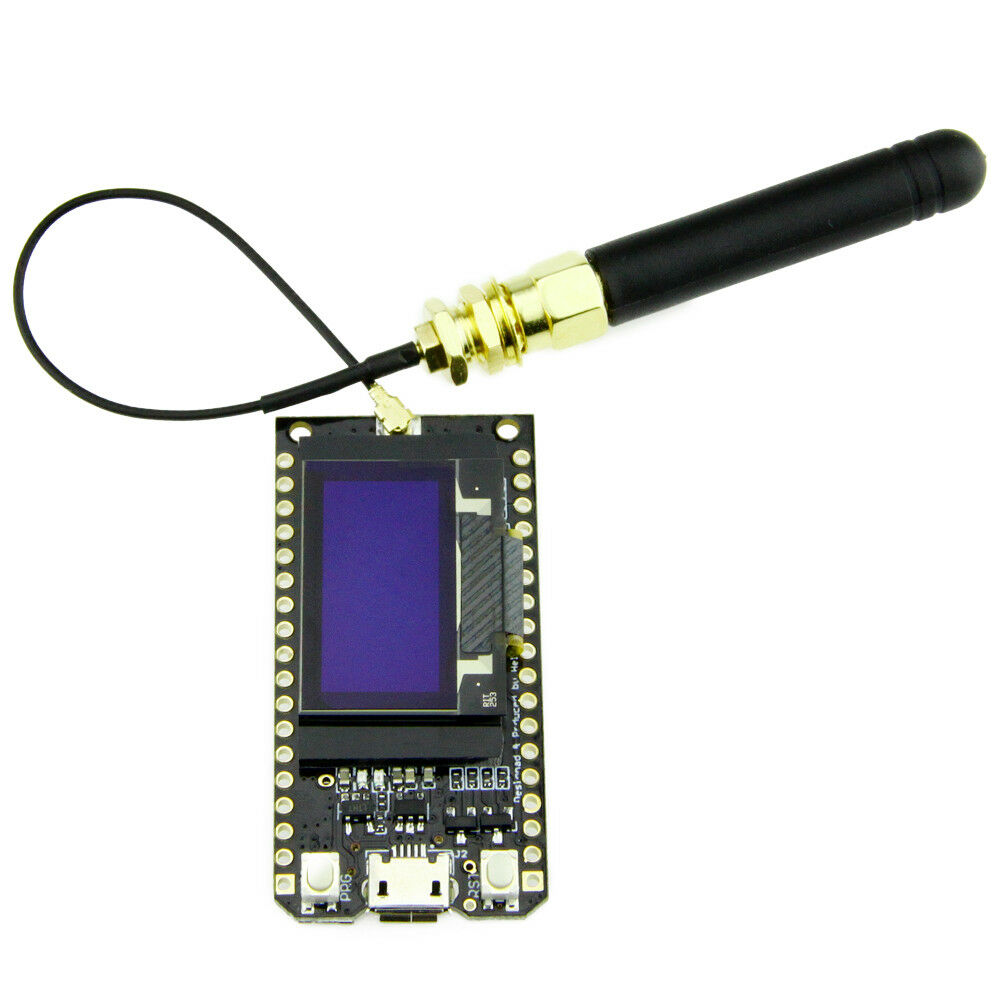
\includegraphics[width=0.33\linewidth]{figuras/lora32.png}
    \caption{\gls{esp32} TTGO \gls{lora}32}
    \label{fig:lora32}
\end{figure}

Do ponto de vista das interfaces de comunicação, o \gls{esp32} suporta nativamente \gls{i2c}, \gls{uart} e \gls{spi}, além da geração de sinais \gls{pwm}, o que o torna adequado para aplicações de controlo de atuadores e aquisição de dados de sensores heterogéneos. O módulo disponibiliza também conectividade sem fios através de \gls{wifi} e \emph{bluetooth}, que, embora não tenham sido utilizados diretamente neste trabalho, representam uma mais-valia para cenários futuros, como a monitorização remota via redes locais ou a configuração simplificada de parâmetros através de dispositivos móveis.  

O \emph{display} \gls{oled} incorporado revelou-se particularmente útil durante a fase de testes e validação, ao permitir monitorizar em tempo real o estado do sistema. Através dele foi possível confirmar a receção de dados provenientes de sensores, a correta execução de comandos de controlo e a integridade das mensagens trocadas via \gls{lora}. Este recurso facilitou o processo de \emph{debug} e reduziu a dependência de sistemas de monitorização externos, acelerando a fase de desenvolvimento.  

Outro aspeto relevante é a vasta comunidade de suporte e o ecossistema de bibliotecas disponíveis para o \gls{esp32}, tanto no ambiente Arduino como em \emph{frameworks} mais avançadas, como a \gls{esp-idf}, que constitui a framework oficial de desenvolvimento disponibilizada pela Espressif programável em C. Esta característica contribui para uma maior fiabilidade no desenvolvimento, reduzindo riscos de integração e permitindo concentrar o esforço na implementação da arquitetura modular proposta para o \gls{usv}.

Em síntese, o módulo TTGO \gls{lora}32 constituiu uma plataforma robusta, versátil e de fácil integração, adequando-se não apenas às exigências do desenvolvimento deste protótipo de \gls{usv}, mas também oferecendo capacidade de evolução para cenários mais complexos, como a execução de algoritmos de navegação autónoma em tempo real ou a integração com sistemas de monitorização distribuídos.

\subsection{Ambiente de Programação}
\label{subsec:ambiente-programacao}

O desenvolvimento do \emph{software} para o protótipo do \gls{usv} foi realizado recorrendo ao ambiente de programação PlatformIO, integrado no editor Visual Studio Code. Esta escolha deve-se às vantagens oferecidas pelo PlatformIO, nomeadamente a gestão centralizada de bibliotecas e o controlo de versões das mesmas, a configuração automatizada do ambiente de compilação e a possibilidade de integração com múltiplos \emph{frameworks} de desenvolvimento.  

Um exemplo claro destas funcionalidades pode ser observado no ficheiro de configuração \texttt{platformio.ini}. Este ficheiro define todas as dependências e parâmetros necessários para compilar e carregar o projeto, assegurando que qualquer programador envolvido no desenvolvimento utiliza exatamente as mesmas versões de bibliotecas e definições de compilação. A Listagem \ref{lst:platformio} mostra um exemplo de um ficheiro de configuração do PlatformIO.

\lstinputlisting[caption={Exemplo de ficheiro \texttt{platformio.ini} utilizado no projeto}, label={lst:platformio}, style=BetterCPP]{code/minimal/exampleplatformIO.ini}

Neste caso, a secção \texttt{[env:ttgo-lora32-v1]} especifica o ambiente de compilação direcionado para a placa TTGO \gls{lora}32, fixando a versão da plataforma \gls{esp32} (\texttt{espressif32@$\sim$5.0.0}) e o \emph{framework} (\texttt{arduino}). A diretiva \texttt{lib\_deps} lista todas as bibliotecas necessárias ao projeto, juntamente com a versão exata de cada uma. Assim, bibliotecas como \texttt{Adafruit SSD1306}, \texttt{LoRa} ou \texttt{TinyGPSPlus} são automaticamente descarregadas e mantidas consistentes em qualquer máquina de desenvolvimento, evitando problemas de incompatibilidade entre versões.  

Este mecanismo garante que o projeto é reprodutível e portável, pois basta clonar o repositório e executar a compilação para obter um ambiente idêntico, sem necessidade de configurar manualmente as bibliotecas ou dependências.

No âmbito deste projeto, foi utilizada a \emph{framework} Arduino do PlatformIO, pela sua simplicidade e pela ampla disponibilidade de bibliotecas compatíveis com o \gls{esp32}. Alternativamente, o \gls{esp-idf} poderia ter sido utilizado, oferecendo maior controlo de baixo nível e otimizações de desempenho, mas a sua maior complexidade tornaria o ciclo de desenvolvimento menos ágil. Assim, a opção pelo ecossistema Arduino mostrou-se mais adequada à prototipagem rápida e à integração de múltiplos sensores e interfaces de comunicação.  

Para além destas ferramentas, foi também utilizado o sistema de controlo de versões Git, com integração em repositório remoto público (\emph{open source}) no GitHub \cite{github-usv}. Este processo assegurou a rastreabilidade das alterações, a organização das diferentes versões do código e a possibilidade de colaboração futura.  

Embora o desenvolvimento principal tenha sido efetuado no Visual Studio Code com o suporte do PlatformIO, foram também realizados testes complementares na Arduino IDE, devido à sua simplicidade na programação inicial do \gls{esp32} e na verificação rápida da compatibilidade das bibliotecas utilizadas.  

Em síntese, a combinação destas ferramentas permitiu estabelecer um ambiente de desenvolvimento robusto, flexível e adaptado às exigências do projeto, ao mesmo tempo que garantiu escalabilidade e reprodutibilidade para trabalhos futuros.

\section{Implementação de \emph{Hardware}}
\label{sec:implementacao-hardware}

A implementação do \emph{\emph{hardware}} do sistema desenvolvido nesta \gls{tfm} assenta numa arquitetura modular, representada de forma esquemática na Figura \ref{fig:placeholder}. Tal como no projeto realizado em \cite{didactic-robot-thesis}, procurou-se manter uma estrutura clara e escalável, onde cada componente desempenha um papel bem definido e comunica com a unidade central de forma eficiente.  

O núcleo do sistema é constituído pelo microcontrolador \gls{esp32}, responsável por coordenar a execução das tarefas de controlo, comunicação e aquisição de dados. Através do barramento \gls{i2c}, o \gls{esp32} comunica com um expansor, responsável pela distribuição dos sinais de controlo e pela interface com os diferentes periféricos \gls{pwm}. Este dispositivo disponibiliza 16 canais adicionais de saída a partir de apenas dois pinos de comunicação \gls{i2c} (SDA e SCL), sendo ainda possível encadear múltiplos expansores para aumentar o número de canais disponíveis. Esta solução permite ultrapassar a limitação do número de pinos físicos do microcontrolador, assegurando a escalabilidade do sistema e reduzindo simultaneamente a complexidade das interligações elétricas, o que simplifica a integração de novos módulos funcionais.

Esta representação global serve como ponto de partida para a descrição detalhada apresentada nas subseções seguintes, onde são abordadas individualmente a integração dos propulsores, a utilização dos sensores, os módulos de comunicação e a conceção da \gls{pcb}.

\subsection{Integração dos Propulsores}
\label{subsec:integracao-propulsores}

A propulsão do \gls{usv} é assegurada por dois propulsores elétricos independentes, cada um alimentado por uma bateria dedicada de 12 V. Esta configuração garante uma fonte de energia estável e suficientemente dimensionada para fornecer a corrente necessária ao funcionamento contínuo dos motores, reduzindo simultaneamente o risco de sobrecarga caso ambos fossem alimentados por uma única bateria.  

A descrição detalhada das características dos motores e do respetivo sistema de controlo eletrónico encontra-se apresentada na Secção \ref{sec:motor}, enquanto o princípio de funcionamento dos \gls{esc} é explicado na Secção \ref{sec:esc}. Aqui, foca-se a forma como esses componentes foram efetivamente integrados no protótipo desenvolvido.  

Cada propulsor encontra-se ligado ao respetivo \gls{esc}, responsável por converter os sinais de controlo recebidos em impulsos elétricos adequados ao motor \emph{brushless}. Tal como descrito anteriormente, o controlo é realizado por sinais de \gls{pwm}, sendo que, no protótipo implementado, o propulsor esquerdo foi ligado ao canal 14 do expansor, enquanto o propulsor direito foi associado ao canal 15. Apesar desta atribuição, qualquer outro canal disponível poderia ser utilizado, uma vez que a correspondência é definida ao nível do \emph{software}.  

O funcionamento dos motores segue o princípio explicado na Secção \ref{sec:esc}, em que a largura do pulso de \gls{pwm} define o sentido e a intensidade da rotação. Esta abordagem permite um controlo independente de cada propulsor, possibilitando tanto movimentos de translação em linha reta como manobras de rotação em torno do próprio eixo, aumentando significativamente a manobrabilidade da embarcação.  

No que respeita aos testes, cada motor foi inicialmente verificado de forma individual, em conjunto com o seu respetivo \gls{esc}, assegurando a correta resposta a diferentes larguras de pulso, a ausência de falhas de comunicação e a estabilidade térmica durante o funcionamento contínuo. Apenas após a validação isolada de cada propulsor se procedeu à sua integração conjunta no sistema, confirmando a coerência do funcionamento em paralelo e a capacidade de executar manobras de coordenação.  

Esta estratégia de integração modular e progressiva assegura que cada propulsor pode ser controlado e validado de forma independente, ao mesmo tempo que garante a escalabilidade do sistema, permitindo a futura adição de mais motores ou a substituição dos atuais sem alterações significativas à arquitetura global.

\subsection{Sensores}
\label{subsec:sensores}

Nesta subseção são descritos os principais sensores integrados no \gls{usv}, responsáveis pela recolha de dados de navegação e monitorização ambiental. São apresentados o \gls{imu}, para determinação do \emph{yaw}, \emph{pitch} e \emph{roll}, e o módulo \gls{gps}, para aquisição de posição geográfica. Adicionalmente, discutem-se aspetos de integração elétrica e física relevantes para o funcionamento estável do sistema.

\subsubsection{\acrfull{imu}}

Para a determinação do \emph{yaw}, \emph{pitch} e \emph{roll} do \gls{usv}, foi utilizado um \gls{imu} baseado no sensor ICM-20948, ilustrado na Figura \ref{fig:imu}. Este dispositivo integra num único chip um acelerómetro de três eixos, um giroscópio de três eixos e um magnetómetro de três eixos, totalizando nove graus de liberdade (9-DOF \emph{gyro-stabilized eCompass} \cite{9dof}). 

\begin{figure}[H]
    \centering
    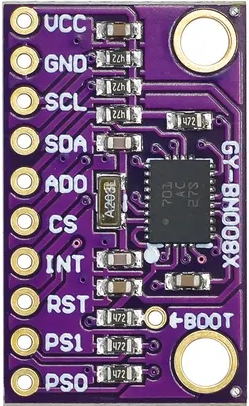
\includegraphics[width=0.25\linewidth]{figuras/imu-icm.jpg}
    \caption{\gls{imu} ICM-20948 utilizada no protótipo}
    \label{fig:imu}
\end{figure}

A combinação destes sensores permite medir acelerações lineares, taxas de rotação e intensidade do campo magnético terrestre, fornecendo assim dados fundamentais para o cálculo do \emph{yaw},  \emph{pitch} e \emph{roll}.

Em termos de integração física, o módulo \gls{imu} foi ligado ao microcontrolador \gls{esp32} através do barramento \gls{i2c}, utilizando os pinos SDA e SCL. No protótipo, foram atribuídos os pinos GPIO 21 (SDA) e GPIO 22 (SCL), respetivamente, recorrendo a uma frequência de comunicação de 400 kHz (\emph{I2C Fast Mode}). Esta interface garante uma comunicação fiável e de elevada velocidade, adequada para a leitura periódica dos dados dos nove eixos.

O ICM-20948 suporta dois endereços \gls{i2c} distintos (0x68 e 0x69), selecionáveis via configuração de \emph{hardware}, o que possibilita a integração simultânea de múltiplos módulos no mesmo barramento, caso seja necessário. No presente projeto, foi utilizada a configuração por omissão (0x68).  

A ligação elétrica do módulo foi realizada diretamente à linha regulada de 3.3~V fornecida pelo \gls{esp32}, estabelecendo-se também a referência comum de massa (GND). Esta configuração garante compatibilidade elétrica entre os dispositivos e elimina a necessidade de conversores de nível lógico, uma vez que tanto o \gls{esp32} como o ICM-20948 operam nativamente a 3.3~V.

O módulo foi montado em proximidade com a unidade de processamento central, dentro da caixa estanque, de forma a reduzir o comprimento dos cabos e minimizar a suscetibilidade a ruídos elétricos. A posição física do sensor foi escolhida de modo a manter o alinhamento dos seus eixos com a estrutura da embarcação, simplificando assim a interpretação dos dados brutos.  

Embora o processo de calibração e compensação de erros seja abordado posteriormente na Secção \ref{sec:implementacao-software}, é importante referir que, a nível de \emph{hardware}, a disposição do sensor e a utilização de ligações curtas e estáveis contribuem para a redução de erros sistemáticos, nomeadamente ruído eletromagnético e interferência cruzada entre sinais.  
    
\subsubsection{\acrfull{gps}}

Para a determinação da posição geográfica do \gls{usv}, foi utilizado o módulo BN-880 \gls{gps}, ilustrado na Figura \ref{fig:gps}. Este recetor integra um chip de posicionamento GNSS e uma antena cerâmica incorporada, sendo amplamente utilizado em aplicações embarcadas devido à sua elevada sensibilidade e ao baixo tempo de aquisição de sinal.  

\begin{figure}[H]
    \centering
    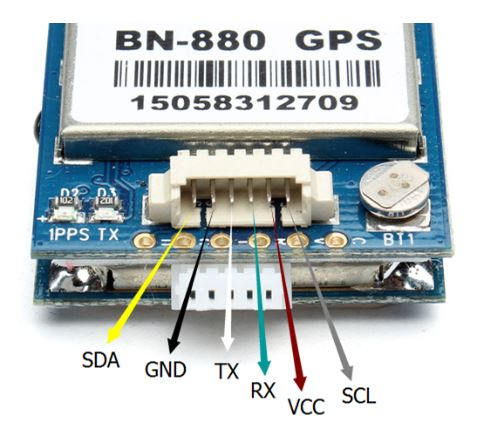
\includegraphics[width=0.4\linewidth]{figuras/BN-880-pinout.jpg}
    \caption{Módulo \gls{gps} BN-880 utilizado no protótipo e respetivo \emph{pinout}}
    \label{fig:gps}
\end{figure}

O módulo \gls{gps} disponibiliza os dados em formato \gls{nmea} \cite{nmea}, um padrão amplamente adotado para a transmissão de coordenadas de latitude, longitude, velocidade e tempo. Estes dados são enviados através de uma interface série \gls{uart}, que estabelece comunicação direta entre o módulo e o microcontrolador.  

No entanto, dado que a porta série principal do \gls{esp32} foi reservada para tarefas de \emph{debug} e monitorização via USB, recorreu-se a um conversor \gls{i2c}-\gls{uart} (SC16IS750), que permitiu a criação de uma porta série adicional a partir do barramento \gls{i2c}. Esta solução garantiu a integração do \gls{gps} sem comprometer a disponibilidade da interface série nativa do \gls{esp32}, mantendo a arquitetura modular e expansível do sistema.  

Um aspeto crítico na integração deste módulo prende-se com a compatibilidade elétrica. Embora o BN-880 seja alimentado a 5 V, o \gls{esp32} opera a 3.3 V nos seus pinos de entrada/saída digitais. Para evitar danos no microcontrolador e assegurar a comunicação fiável, foi introduzido um conversor de nível lógico, responsável por adaptar os sinais da interface \gls{uart} entre os dois dispositivos.  

A alimentação do módulo é assegurada diretamente pela linha de 5 V do sistema, enquanto as ligações de dados (TX e RX) passam pelo conversor de nível lógico antes de chegar ao \gls{esp32}. Esta configuração garante a integridade do sinal e a proteção dos módulos. As ligações elétricas detalhadas podem ser observadas no Anexo \ref{anexo:pcb}, na Figura \ref{fig:esquematica-gps}, que apresenta a esquemática correspondente.  

Tal como o \gls{imu}, o módulo \gls{gps} foi instalado no interior da caixa estanque, com especial atenção à orientação da antena integrada, de forma a manter visibilidade direta com o céu e reduzir obstruções ao sinal.

\subsection{Comunicação}

A comunicação entre o \gls{usv} e a estação remota é assegurada pela tecnologia \acrfull{lora}, integrada no próprio \gls{esp32} TTGO \gls{lora}32, que incorpora o transceptor Semtech SX1276. Esta solução permitiu simplificar a arquitetura de \emph{\emph{hardware}}, eliminando a necessidade de módulos externos dedicados de rádio e garantindo ao mesmo tempo baixo consumo energético e elevada robustez em cenários de operação remota.  

A configuração do transceptor \gls{lora} foi realizada de acordo com a regulamentação europeia, utilizando uma frequência de operação de 866 MHz. 

O sistema foi configurado para operar com um \emph{Spreading Factor} de 12, que maximiza o alcance da comunicação ao custo de um \emph{bitrate} mais baixo. Apesar de não ter sido modificada no protótipo, a biblioteca \gls{lora} permite também ajustar parâmetros como a potência de transmissão, a largura de banda e o esquema de codificação, o que poderá ser explorado em trabalhos futuros para otimizar o compromisso entre alcance, robustez e eficiência energética.  

A comunicação pode ser utilizada para dois propósitos principais:  

\begin{enumerate}
    \item Comandos remotos, que foram implementados no âmbito deste trabalho, consistem na receção de instruções provenientes da estação remota. Estes comandos permitem tanto a atualização de rotas sob a forma de \emph{waypoints} como a navegação manual, através de ordens de movimento direto (avante e atrás), lateral (esquerda e direita) e paragem. A implementação destes comandos garante a possibilidade de alternar entre controlo autónomo e intervenção manual sempre que necessário.  
    \item Telemetria, que consiste no envio periódico de dados essenciais para a monitorização do sistema, incluindo posição \gls{gps}, orientação obtida pelo \gls{imu}, estado da bateria e modo de controlo ativo (manual ou automático). Esta funcionalidade não foi implementada na presente fase do trabalho, encontrando-se prevista para desenvolvimentos futuros.  
\end{enumerate}

\subsection{\acrfull{pcb}}
\label{subsec:pcb}

Com o objetivo de integrar todos os módulos do sistema de forma compacta e fiável, foi desenvolvida uma \gls{pcb} dedicada, que reúne numa única placa todos os elementos de controlo, aquisição e comunicação do protótipo do \gls{usv}. A centralização numa única \gls{pcb} reduz significativamente a complexidade da cablagem, minimiza possíveis falhas de ligação e facilita a montagem, manutenção e escalabilidade do sistema.  

Na sua conceção, a placa incorpora diferentes blocos funcionais. O processamento central é assegurado pelo módulo TTGO \gls{lora}32, baseado no microcontrolador \gls{esp32}, que tem a responsabilidade de gerar sinais \gls{pwm}, gerir a comunicação via \gls{i2c}, \gls{uart} e \gls{lora}, e garantir a ligação ao sistema através de uma antena dedicada. O controlo dos motores é realizado por um expansor PCA9685, que disponibiliza até 16 canais de \gls{pwm}, dos quais dois foram configurados para comandar os propulsores através dos respetivos \gls{esc}.  

No que respeita à navegação, o recetor \gls{gps} BN-880 foi integrado no sistema através de um conversor SC16IS750, que atua como ponte entre a interface \gls{uart} do módulo e o barramento \gls{i2c}, permitindo a sua comunicação com o microcontrolador sem comprometer a arquitetura modular. Complementarmente, o sensor \gls{imu} ICM-20948, também conectado por \gls{i2c}, assegura medições contínuas de aceleração, velocidade angular e intensidade do campo magnético nos três eixos, fundamentais para a estimativa da orientação do veículo.  

Por fim, a gestão de energia foi contemplada através da inclusão de conectores específicos para a entrada de energia principal a 12~V, interruptores de corte que permitem desligar o sistema de forma segura e \gls{led} indicadores que fornecem feedback visual sobre o estado de funcionamento.  

A Figura \ref{fig:pcb-esquematica-vs-real} ilustra a comparação entre a esquemática desenvolvida e a implementação física da placa.

\begin{figure}[H]
    \centering
    \begin{minipage}{0.45\linewidth}
        \centering
        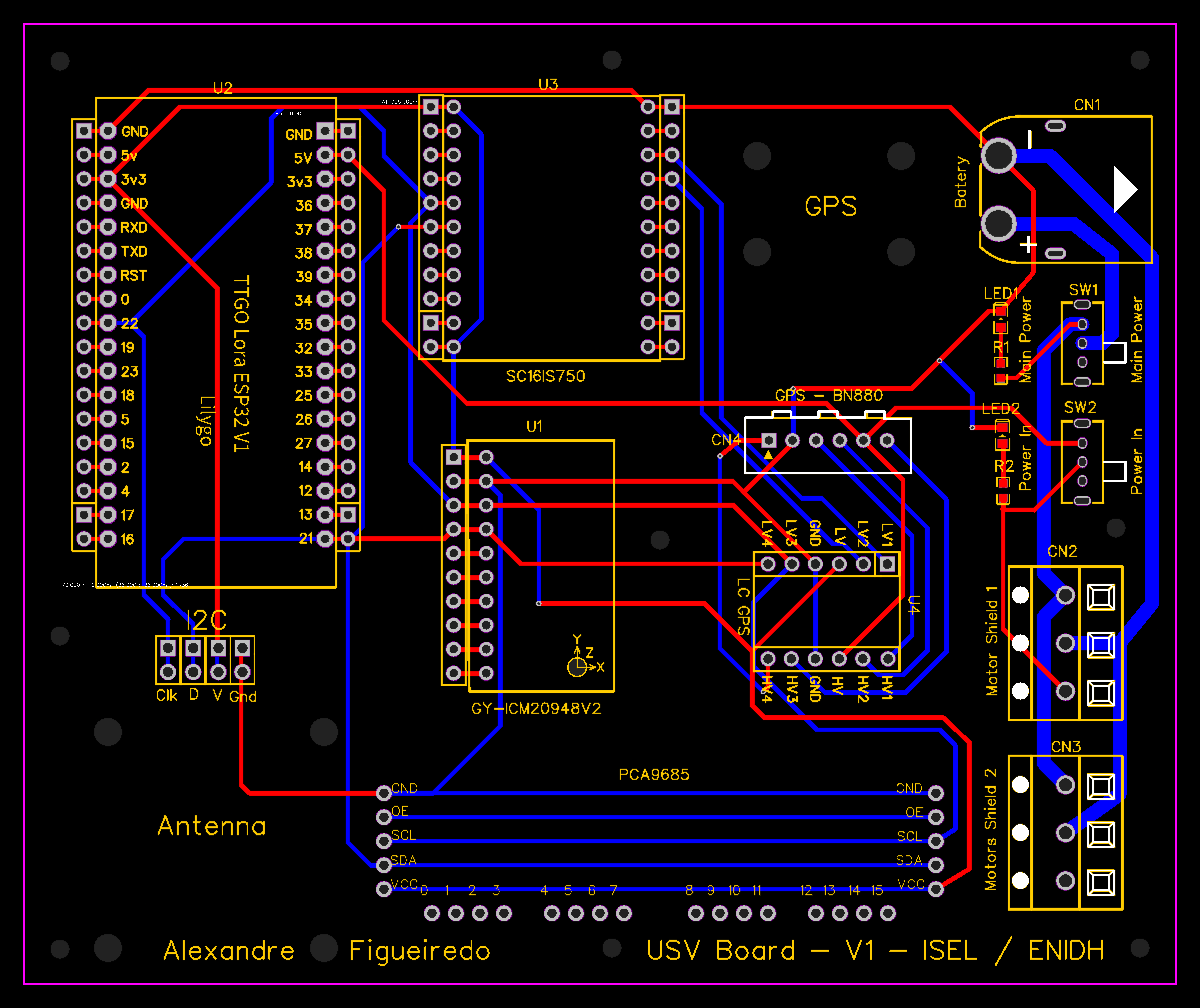
\includegraphics[width=0.80\linewidth]{figuras/PCB_PCB_USV-Board_2025-09-21.png}
        \caption*{(A) \emph{Layout} da PCB}
    \end{minipage}
    \hfill
    \begin{minipage}{0.40\linewidth}
        \centering
        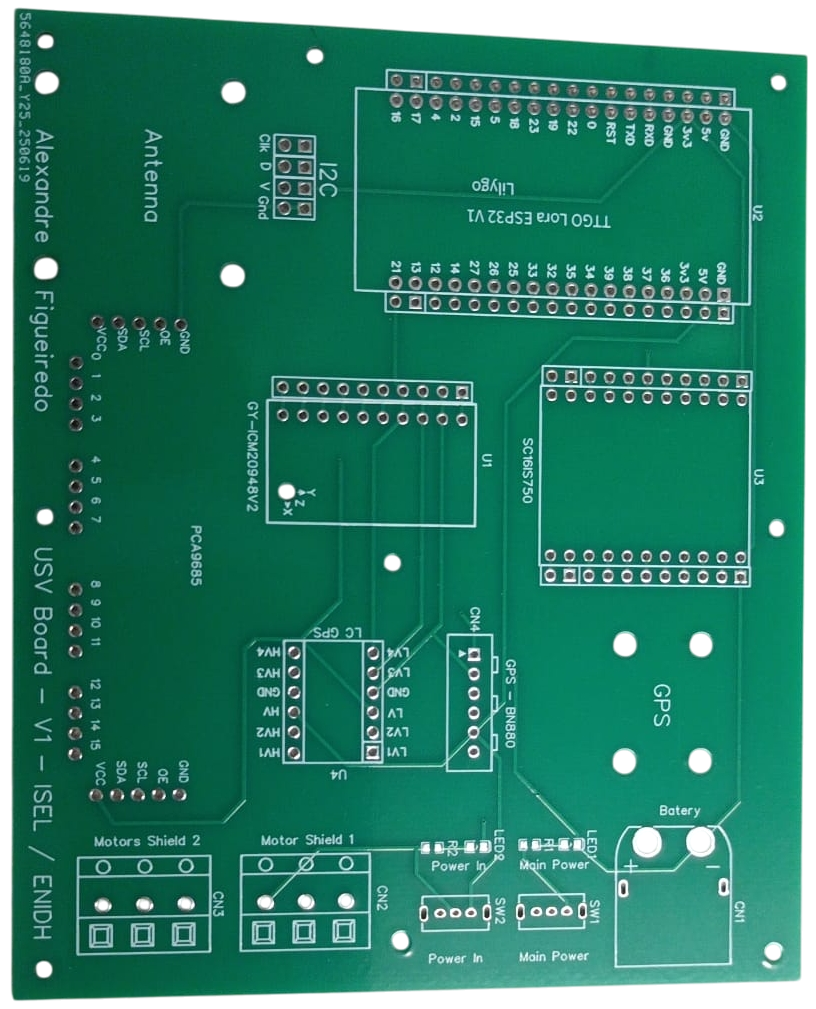
\includegraphics[width=0.80\linewidth,angle=90]{figuras/pcb-real.png}
        \caption*{(B) Implementação real}
    \end{minipage}
    \caption{Comparação entre a esquemática (A) e a implementação física (B) da \gls{pcb}}
    \label{fig:pcb-esquematica-vs-real}
\end{figure}

As esquemáticas completas encontram-se documentadas no Anexo \ref{anexo:pcb}, permitindo uma análise detalhada de cada ligação elétrica. A versão montada da \gls{pcb} encontra-se representada na Figura \ref{fig:pcb-final}, onde é possível identificar a disposição dos principais módulos e as camadas de interligação.  

\begin{figure}[H]
    \centering
    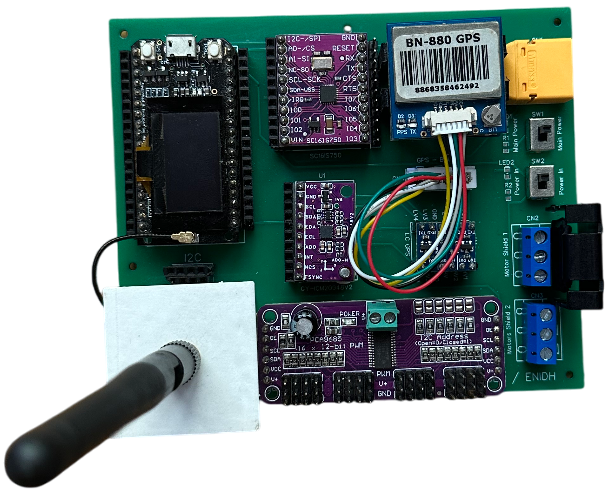
\includegraphics[width=0.5\linewidth]{figuras/pcb-final.png}
    \caption{Versão montada da \gls{pcb} desenvolvida para o protótipo do \gls{usv}}
    \label{fig:pcb-final}
\end{figure}

Em suma, a integração de todos os módulos numa única \gls{pcb} permitiu não só simplificar o design global do sistema, mas também garantir maior fiabilidade elétrica e reduzir a probabilidade de falhas por mau contacto ou cablagem incorreta. Esta abordagem aumenta a robustez do protótipo e facilita a sua replicação em versões futuras.

\section{Implementação de \emph{Software}}
\label{sec:implementacao-software}

A implementação de \emph{software} constituiu a camada lógica do sistema desenvolvido, responsável por coordenar a interação entre os diferentes módulos de \emph{\emph{hardware}}, assegurar o processamento em tempo real dos dados de sensores, gerir a comunicação sem fios e aplicar os algoritmos de navegação. Esta camada foi concebida de forma modular, permitindo que cada componente seja desenvolvido, testado e substituído de forma independente, sem comprometer a integridade do sistema global.  

O código foi estruturado para garantir três requisitos principais: funcionamento não bloqueante, escalabilidade e reutilização. O primeiro requisito assegura que todas as tarefas críticas, como leitura de sensores, controlo dos motores e receção de comandos, são executadas sem interrupções prolongadas, preservando a responsividade do sistema. O segundo requisito garante que novos módulos ou algoritmos de controlo podem ser facilmente integrados, acompanhando a evolução do protótipo. O terceiro requisito promove a portabilidade do código para outros projetos semelhantes, mantendo a mesma filosofia modular que guiou a implementação do Robot Didático \cite{didactic-robot-thesis}.  

Importa ainda destacar que todo o código desenvolvido no âmbito desta \gls{tfm} foi disponibilizado em regime de \emph{open source}, encontrando-se acessível num repositório público de controlo de versões na plataforma GitHub \cite{github-usv}. Esta decisão assegura não apenas a transparência e reprodutibilidade científica, mas também a possibilidade de reutilização, extensão e validação por parte de outros estudantes, investigadores, profissionais da área e qualquer curioso.

Ao longo desta secção são descritos os principais aspetos da implementação de \emph{software}, incluindo a integração dos subsistemas no ciclo principal na Subsecção~\ref{sec:integracao}, a arquitetura modular do código na Subsecção~\ref{subsec:arquitetura-codigo}, o controlo dos motores na Subsecção~\ref{subsec:controlo-de-motores}, a leitura e processamento dos sensores na Subsecção~\ref{subsec:processamento-sensores} e a comunicação via \gls{lora} com mensagens estruturadas em \emph{Protobuf} na Subsecção~\ref{subsec:comunicacao-lora}. Estes elementos, em conjunto, constituem a base funcional que permite ao veículo operar de forma autónoma ou manual, com monitorização e controlo em tempo real.

\subsection{Integração do Sistema}
\label{sec:integracao}

A integração do sistema foi concebida de forma modular, com o objetivo de simplificar o desenvolvimento e permitir que novos utilizadores ou projetos derivados possam reutilizar o código com um esforço mínimo. A interface de utilização resume-se à inicialização do objeto principal \texttt{\gls{usv}} e à execução do método \texttt{loop()}, que coordena todos os subsistemas. Os sensores disponibilizam métodos dedicados para aceder aos dados mais recentes (e.g. \texttt{getGPSData()}, \texttt{getIMUData()}), garantindo uma utilização intuitiva e não bloqueante.  

\subsubsection{Estrutura do Código Principal}

O código principal (contido no ficheiro \texttt{main\_usv.cpp}) organiza-se em duas funções fundamentais: \texttt{setup()}, responsável pela inicialização de todos os módulos (sensores, comunicação, propulsores e controladores), e \texttt{loop()}, que executa repetidamente o ciclo de controlo. A execução do \texttt{loop()} do objeto \texttt{\gls{usv}} é suficiente para garantir a atualização contínua de sensores, o envio de telemetria, a receção de comandos e o controlo dos motores. A lógica interna foi desenhada para operar de forma assíncrona, evitando chamadas bloqueantes que pudessem comprometer a responsividade do sistema. 

A Listagem \ref{lst:main-usv-cpp} apresenta o código completo do ficheiro \texttt{main\_usv.cpp}, ilustrando a simplicidade da interface de controlo.

\lstinputlisting[caption=Estrutura principal do programa do \gls{usv}, label={lst:main-usv-cpp}, style=BetterCPP]{code/minimal/main_usv.cpp}

É importante destacar que os dados provenientes do \gls{gps} e da \gls{imu} são processados de forma independente. A obtenção destas informações é realizada explicitamente através das chamadas aos métodos \texttt{getGPSData()} e \texttt{getIMUData()}, nas linhas 27 e 28 do código, respetivamente. Esta abordagem reflete uma decisão arquitetural relevante, pois garante que o objeto \texttt{USV} não está rigidamente acoplado a implementações específicas de sensores, mas antes a interfaces genéricas que fornecem dados estruturados de posicionamento e orientação.  

Desta forma, a substituição ou atualização de sensores pode ser efetuada sem necessidade de alterar a lógica central do sistema, preservando a modularidade e a escalabilidade do \emph{software}. A profundidade desta estratégia de abstração e independência sensorial é analisada em maior detalhe na Subsecção~\ref{subsec:processamento-sensores}, onde se descrevem os mecanismos de aquisição e processamento de dados dos sensores.

\subsubsection{Sincronização de Sensores, Motores e Comunicação}  

A atualização dos sensores é realizada periodicamente, com cada módulo a gerir internamente a sua própria leitura. O \gls{gps}, através da classe \texttt{GPS\_BN880}, descodifica continuamente as mensagens \gls{nmea} recebidas via ponte \gls{i2c}-\gls{uart}, enquanto o \gls{imu} (\texttt{IMU\_ICM\_20948}) atualiza os valores de aceleração, rotação e orientação utilizando o filtro de Madgwick \cite{madgwick-filter}. Os propulsores são controlados via \gls{pwm} gerado pelo expansor, com os valores definidos pela lógica de navegação implementada na classe \texttt{Control}. Paralelamente, a comunicação \gls{lora}, encapsulada nas classes \texttt{LoRaDuplex} e \texttt{LoRaProto}, trata de forma não bloqueante tanto o envio periódico de telemetria como a receção de pacotes de controlo. Esta abordagem garante que nenhum módulo interrompe a execução do ciclo principal, assegurando a fluidez da operação em tempo real.

\subsubsection{Testes Incrementais}

A validação do sistema foi realizada de forma incremental, seguindo uma estratégia de integração progressiva. Numa primeira fase foram testados os motores de forma isolada, validando a geração de sinais \gls{pwm}, o processo de armamento dos \gls{esc} e a resposta dos propulsores. Posteriormente, os sensores foram integrados individualmente, confirmando a calibração do \gls{imu} e a receção estável de coordenadas \gls{gps}. Numa fase seguinte, foi estabelecida a comunicação via \gls{lora}, assegurando a transmissão de telemetria e a receção de comandos em tempo real. Finalmente, todos os módulos foram integrados no sistema completo, testando a coerência do funcionamento conjunto, incluindo a execução de rotas automáticas baseadas em \emph{waypoints} e a alternância entre modos manual e automático.

Em síntese, a arquitetura de \emph{software} foi desenhada para ser modular, escalável e de fácil utilização, permitindo que qualquer utilizador possa controlar o \gls{usv} com apenas algumas chamadas de alto nível, enquanto a lógica interna garante a sincronização e integração de todos os subsistemas de forma transparente.

\subsection{Arquitetura do Código}
\label{subsec:arquitetura-codigo}

A arquitetura de \emph{software} foi concebida de forma modular, seguindo princípios de encapsulamento e separação de responsabilidades. Cada componente do sistema foi implementado numa biblioteca própria, organizada em \emph{packages} correspondentes às suas funções principais, como propulsão, sensores, comunicação e controlo. Esta abordagem modular facilita a manutenção, promove a reutilização do código e assegura a escalabilidade do sistema, permitindo que novos sensores ou atuadores possam ser integrados com alterações mínimas à base existente.  

A Figura~\ref{fig:uml-simplificado} apresenta um diagrama \gls{uml} simplificado que ilustra a arquitetura do sistema e as interações entre as suas classes principais (para diagramas mais complexos ver Anexo \ref{anexo:diagramas-de-classes}). 

\begin{figure}[H]
  \centering
  \resizebox{\textwidth}{!}{%
    % generated by Plantuml 1.2024.3       
\definecolor{plantucolor0000}{RGB}{255,255,255}
\definecolor{plantucolor0001}{RGB}{0,0,0}
\definecolor{plantucolor0002}{RGB}{238,238,238}
\definecolor{plantucolor0003}{RGB}{221,221,221}
\definecolor{plantucolor0004}{RGB}{204,204,204}
\definecolor{plantucolor0005}{RGB}{187,187,187}
\begin{tikzpicture}[yscale=-1
,pstyle0/.style={color=black,fill=white,line width=1.0pt}
,pstyle1/.style={color=black,line width=1.0pt}
,pstyle6/.style={color=black,fill=black,line width=1.0pt}
]
\draw[pstyle0] (794.5pt,11.602pt) -- (917.9187pt,11.602pt) arc(270:360:3.75pt)  -- (927.4187pt,36.6699pt) -- (974.5pt,36.6699pt) arc(270:360:2.5pt)  -- (977pt,349.102pt) arc(0:90:2.5pt)  -- (794.5pt,351.602pt) arc(90:180:2.5pt)  -- (792pt,14.102pt) arc(180:270:2.5pt) ;
\draw[pstyle1] (792pt,36.6699pt) -- (927.4187pt,36.6699pt);
\node at (796pt,13.602pt)[below right,color=black]{\textbf{Robot Didático}};
\draw[color=black,fill=plantucolor0002,line width=1.0pt] (13.5pt,19.602pt) -- (47.6714pt,19.602pt) arc(270:360:3.75pt)  -- (57.1714pt,44.6699pt) -- (761.5pt,44.6699pt) arc(270:360:2.5pt)  -- (764pt,117.102pt) arc(0:90:2.5pt)  -- (13.5pt,119.602pt) arc(90:180:2.5pt)  -- (11pt,22.102pt) arc(180:270:2.5pt) ;
\draw[pstyle1] (11pt,44.6699pt) -- (57.1714pt,44.6699pt);
\node at (15pt,21.602pt)[below right,color=black]{\textbf{USV}};
\draw[color=black,fill=plantucolor0003,line width=1.0pt] (404.5pt,340.602pt) -- (468.9667pt,340.602pt) arc(270:360:3.75pt)  -- (478.4667pt,365.6699pt) -- (531.5pt,365.6699pt) arc(270:360:2.5pt)  -- (534pt,473.102pt) arc(0:90:2.5pt)  -- (404.5pt,475.602pt) arc(90:180:2.5pt)  -- (402pt,343.102pt) arc(180:270:2.5pt) ;
\draw[pstyle1] (402pt,365.6699pt) -- (478.4667pt,365.6699pt);
\node at (406pt,342.602pt)[below right,color=black]{\textbf{Control}};
\draw[color=black,fill=plantucolor0004,line width=1.0pt] (601pt,428.602pt) -- (665.6727pt,428.602pt) arc(270:360:3.75pt)  -- (675.1727pt,453.6699pt) -- (722pt,453.6699pt) arc(270:360:2.5pt)  -- (724.5pt,606.102pt) arc(0:90:2.5pt)  -- (601pt,608.602pt) arc(90:180:2.5pt)  -- (598.5pt,431.102pt) arc(180:270:2.5pt) ;
\draw[pstyle1] (598.5pt,453.6699pt) -- (675.1727pt,453.6699pt);
\node at (602.5pt,430.602pt)[below right,color=black]{\textbf{Sensors}};
\draw[color=black,fill=plantucolor0005,line width=1.0pt] (181pt,303.602pt) -- (315.2991pt,303.602pt) arc(270:360:3.75pt)  -- (324.7991pt,328.6699pt) -- (325pt,328.6699pt) arc(270:360:2.5pt)  -- (327.5pt,481.102pt) arc(0:90:2.5pt)  -- (181pt,483.602pt) arc(90:180:2.5pt)  -- (178.5pt,306.102pt) arc(180:270:2.5pt) ;
\draw[pstyle1] (178.5pt,328.6699pt) -- (324.7991pt,328.6699pt);
\node at (182.5pt,305.602pt)[below right,color=black]{\textbf{Communication}};
\draw[pstyle0] (848.5pt,295.102pt) arc (180:270:5pt) -- (853.5pt,290.102pt) -- (915.8897pt,290.102pt) arc (270:360:5pt) -- (920.8897pt,295.102pt) -- (920.8897pt,330.1699pt) arc (0:90:5pt) -- (915.8897pt,335.1699pt) -- (853.5pt,335.1699pt) arc (90:180:5pt) -- (848.5pt,330.1699pt) -- cycle;
\draw[pstyle0] (860.5pt,304.6359pt) ellipse (8pt and 8pt);
\node at (860.5pt,304.6359pt)[]{\textbf{\Large C}};
\node at (871.5pt,295.102pt)[below right,color=black]{Robot};
\draw[pstyle1] (849.5pt,319.1699pt) -- (919.8897pt,319.1699pt);
\draw[pstyle1] (849.5pt,327.1699pt) -- (919.8897pt,327.1699pt);
\draw[pstyle0] (830.5pt,215.102pt) arc (180:270:5pt) -- (835.5pt,210.102pt) -- (933.7857pt,210.102pt) arc (270:360:5pt) -- (938.7857pt,215.102pt) -- (938.7857pt,250.1699pt) arc (0:90:5pt) -- (933.7857pt,255.1699pt) -- (835.5pt,255.1699pt) arc (90:180:5pt) -- (830.5pt,250.1699pt) -- cycle;
\draw[pstyle0] (842.5pt,224.6359pt) ellipse (8pt and 8pt);
\node at (842.5pt,224.6359pt)[]{\textbf{\Large C}};
\node at (853.5pt,215.102pt)[below right,color=black]{Movement};
\draw[pstyle1] (831.5pt,239.1699pt) -- (937.7857pt,239.1699pt);
\draw[pstyle1] (831.5pt,247.1699pt) -- (937.7857pt,247.1699pt);
\draw[pstyle0] (847.5pt,135.102pt) arc (180:270:5pt) -- (852.5pt,130.102pt) -- (916.7244pt,130.102pt) arc (270:360:5pt) -- (921.7244pt,135.102pt) -- (921.7244pt,170.1699pt) arc (0:90:5pt) -- (916.7244pt,175.1699pt) -- (852.5pt,175.1699pt) arc (90:180:5pt) -- (847.5pt,170.1699pt) -- cycle;
\draw[pstyle0] (859.5pt,144.6359pt) ellipse (8pt and 8pt);
\node at (859.5pt,144.6359pt)[]{\textbf{\Large C}};
\node at (870.5pt,135.102pt)[below right,color=black]{Motor};
\draw[pstyle1] (848.5pt,159.1699pt) -- (920.7244pt,159.1699pt);
\draw[pstyle1] (848.5pt,167.1699pt) -- (920.7244pt,167.1699pt);
\draw[pstyle0] (808pt,55.102pt) arc (180:270:5pt) -- (813pt,50.102pt) -- (956.4972pt,50.102pt) arc (270:360:5pt) -- (961.4972pt,55.102pt) -- (961.4972pt,90.1699pt) arc (0:90:5pt) -- (956.4972pt,95.1699pt) -- (813pt,95.1699pt) arc (90:180:5pt) -- (808pt,90.1699pt) -- cycle;
\draw[pstyle0] (820pt,64.6359pt) ellipse (8pt and 8pt);
\node at (820pt,64.6359pt)[]{\textbf{\Large C}};
\node at (831pt,55.102pt)[below right,color=black]{MotorController};
\draw[pstyle1] (809pt,79.1699pt) -- (960.4972pt,79.1699pt);
\draw[pstyle1] (809pt,87.1699pt) -- (960.4972pt,87.1699pt);
\draw[pstyle0] (27pt,63.102pt) arc (180:270:5pt) -- (32pt,58.102pt) -- (79.2148pt,58.102pt) arc (270:360:5pt) -- (84.2148pt,63.102pt) -- (84.2148pt,98.1699pt) arc (0:90:5pt) -- (79.2148pt,103.1699pt) -- (32pt,103.1699pt) arc (90:180:5pt) -- (27pt,98.1699pt) -- cycle;
\draw[pstyle0] (39pt,72.6359pt) ellipse (8pt and 8pt);
\node at (39pt,72.6359pt)[]{\textbf{\Large C}};
\node at (50pt,63.102pt)[below right,color=black]{USV};
\draw[pstyle1] (28pt,87.1699pt) -- (83.2148pt,87.1699pt);
\draw[pstyle1] (28pt,95.1699pt) -- (83.2148pt,95.1699pt);
\draw[pstyle0] (144pt,63.102pt) arc (180:270:5pt) -- (149pt,58.102pt) -- (355.9463pt,58.102pt) arc (270:360:5pt) -- (360.9463pt,63.102pt) -- (360.9463pt,98.1699pt) arc (0:90:5pt) -- (355.9463pt,103.1699pt) -- (149pt,103.1699pt) arc (90:180:5pt) -- (144pt,98.1699pt) -- cycle;
\draw[pstyle0] (156pt,72.6359pt) ellipse (8pt and 8pt);
\node at (156pt,72.6359pt)[]{\textbf{\Large C}};
\node at (167pt,63.102pt)[below right,color=black]{MovementTwoThrusters};
\draw[pstyle1] (145pt,87.1699pt) -- (359.9463pt,87.1699pt);
\draw[pstyle1] (145pt,95.1699pt) -- (359.9463pt,95.1699pt);
\draw[pstyle0] (421pt,63.102pt) arc (180:270:5pt) -- (426pt,58.102pt) -- (509.7492pt,58.102pt) arc (270:360:5pt) -- (514.7492pt,63.102pt) -- (514.7492pt,98.1699pt) arc (0:90:5pt) -- (509.7492pt,103.1699pt) -- (426pt,103.1699pt) arc (90:180:5pt) -- (421pt,98.1699pt) -- cycle;
\draw[pstyle0] (433pt,72.6359pt) ellipse (8pt and 8pt);
\node at (433pt,72.6359pt)[]{\textbf{\Large C}};
\node at (444pt,63.102pt)[below right,color=black]{Thruster};
\draw[pstyle1] (422pt,87.1699pt) -- (513.7492pt,87.1699pt);
\draw[pstyle1] (422pt,95.1699pt) -- (513.7492pt,95.1699pt);
\draw[pstyle0] (575pt,63.102pt) arc (180:270:5pt) -- (580pt,58.102pt) -- (743.0142pt,58.102pt) arc (270:360:5pt) -- (748.0142pt,63.102pt) -- (748.0142pt,98.1699pt) arc (0:90:5pt) -- (743.0142pt,103.1699pt) -- (580pt,103.1699pt) arc (90:180:5pt) -- (575pt,98.1699pt) -- cycle;
\draw[pstyle0] (587pt,72.6359pt) ellipse (8pt and 8pt);
\node at (587pt,72.6359pt)[]{\textbf{\Large S}};
\node at (598pt,63.102pt)[below right,color=black]{ThrusterController};
\draw[pstyle1] (576pt,87.1699pt) -- (747.0142pt,87.1699pt);
\draw[pstyle1] (576pt,95.1699pt) -- (747.0142pt,95.1699pt);
\draw[pstyle0] (426pt,392.102pt) arc (180:270:5pt) -- (431pt,387.102pt) -- (505.32pt,387.102pt) arc (270:360:5pt) -- (510.32pt,392.102pt) -- (510.32pt,427.1699pt) arc (0:90:5pt) -- (505.32pt,432.1699pt) -- (431pt,432.1699pt) arc (90:180:5pt) -- (426pt,427.1699pt) -- cycle;
\draw[pstyle0] (438pt,401.6359pt) ellipse (8pt and 8pt);
\node at (438pt,401.6359pt)[]{\textbf{\Large C}};
\node at (449pt,392.102pt)[below right,color=black]{Control};
\draw[pstyle1] (427pt,416.1699pt) -- (509.32pt,416.1699pt);
\draw[pstyle1] (427pt,424.1699pt) -- (509.32pt,424.1699pt);
\draw[pstyle0] (615.5pt,472.102pt) arc (180:270:5pt) -- (620.5pt,467.102pt) -- (702.093pt,467.102pt) arc (270:360:5pt) -- (707.093pt,472.102pt) -- (707.093pt,507.1699pt) arc (0:90:5pt) -- (702.093pt,512.1699pt) -- (620.5pt,512.1699pt) arc (90:180:5pt) -- (615.5pt,507.1699pt) -- cycle;
\draw[pstyle0] (627.5pt,481.6359pt) ellipse (8pt and 8pt);
\node at (627.5pt,481.6359pt)[]{\textbf{\Large C}};
\node at (638.5pt,472.102pt)[below right,color=black]{GPSData};
\draw[pstyle1] (616.5pt,496.1699pt) -- (706.093pt,496.1699pt);
\draw[pstyle1] (616.5pt,504.1699pt) -- (706.093pt,504.1699pt);
\draw[pstyle0] (614.5pt,552.102pt) arc (180:270:5pt) -- (619.5pt,547.102pt) -- (703.2492pt,547.102pt) arc (270:360:5pt) -- (708.2492pt,552.102pt) -- (708.2492pt,587.1699pt) arc (0:90:5pt) -- (703.2492pt,592.1699pt) -- (619.5pt,592.1699pt) arc (90:180:5pt) -- (614.5pt,587.1699pt) -- cycle;
\draw[pstyle0] (626.5pt,561.6359pt) ellipse (8pt and 8pt);
\node at (626.5pt,561.6359pt)[]{\textbf{\Large C}};
\node at (637.5pt,552.102pt)[below right,color=black]{IMUData};
\draw[pstyle1] (615.5pt,576.1699pt) -- (707.2492pt,576.1699pt);
\draw[pstyle1] (615.5pt,584.1699pt) -- (707.2492pt,584.1699pt);
\draw[pstyle0] (225pt,347.102pt) arc (180:270:5pt) -- (230pt,342.102pt) -- (275.04pt,342.102pt) arc (270:360:5pt) -- (280.04pt,347.102pt) -- (280.04pt,382.1699pt) arc (0:90:5pt) -- (275.04pt,387.1699pt) -- (230pt,387.1699pt) arc (90:180:5pt) -- (225pt,382.1699pt) -- cycle;
\draw[pstyle0] (237pt,356.6359pt) ellipse (8pt and 8pt);
\node at (237pt,356.6359pt)[]{\textbf{\Large C}};
\node at (248pt,347.102pt)[below right,color=black]{Led};
\draw[pstyle1] (226pt,371.1699pt) -- (279.04pt,371.1699pt);
\draw[pstyle1] (226pt,379.1699pt) -- (279.04pt,379.1699pt);
\draw[pstyle0] (219.5pt,427.102pt) arc (180:270:5pt) -- (224.5pt,422.102pt) -- (280.3588pt,422.102pt) arc (270:360:5pt) -- (285.3588pt,427.102pt) -- (285.3588pt,462.1699pt) arc (0:90:5pt) -- (280.3588pt,467.1699pt) -- (224.5pt,467.1699pt) arc (90:180:5pt) -- (219.5pt,462.1699pt) -- cycle;
\draw[pstyle0] (231.5pt,436.6359pt) ellipse (8pt and 8pt);
\node at (231.5pt,436.6359pt)[]{\textbf{\Large C}};
\node at (242.5pt,427.102pt)[below right,color=black]{LoRa};
\draw[pstyle1] (220.5pt,451.1699pt) -- (284.3588pt,451.1699pt);
\draw[pstyle1] (220.5pt,459.1699pt) -- (284.3588pt,459.1699pt);
\draw[pstyle1] (76pt,103.272pt) ..controls (76pt,161.642pt) and (76pt,312.602pt) .. (76pt,312.602pt) ..controls (76pt,312.602pt) and (673.56pt,312.602pt) .. (830.45pt,312.602pt);
\draw[pstyle1] (848.45pt,312.602pt) -- (830.45pt,306.602pt) -- (830.45pt,318.602pt) -- (848.45pt,312.602pt) -- cycle;
\draw[pstyle1] (324pt,103.362pt) ..controls (324pt,145.762pt) and (324pt,232.602pt) .. (324pt,232.602pt) ..controls (324pt,232.602pt) and (671.58pt,232.602pt) .. (812.25pt,232.602pt);
\draw[pstyle1] (830.25pt,232.602pt) -- (812.25pt,226.602pt) -- (812.25pt,238.602pt) -- (830.25pt,232.602pt) -- cycle;
\draw[pstyle1] (468pt,103.382pt) ..controls (468pt,124.482pt) and (468pt,152.602pt) .. (468pt,152.602pt) ..controls (468pt,152.602pt) and (726.94pt,152.602pt) .. (829.17pt,152.602pt);
\draw[pstyle1] (847.17pt,152.602pt) -- (829.17pt,146.602pt) -- (829.17pt,158.602pt) -- (847.17pt,152.602pt) -- cycle;
\draw[pstyle1] (748.04pt,76.602pt) ..controls (767.75pt,76.602pt) and (770.56pt,76.602pt) .. (789.82pt,76.602pt);
\draw[pstyle1] (807.82pt,76.602pt) -- (789.82pt,70.602pt) -- (789.82pt,82.602pt) -- (807.82pt,76.602pt) -- cycle;
\draw[pstyle1] (96.15pt,80.602pt) ..controls (112.37pt,80.602pt) and (121.79pt,80.602pt) .. (143.91pt,80.602pt);
\draw[pstyle1] (84.15pt,80.602pt) -- (90.15pt,84.602pt) -- (96.15pt,80.602pt) -- (90.15pt,76.602pt) -- (84.15pt,80.602pt) -- cycle;
\draw[pstyle1] (52pt,115.382pt) ..controls (52pt,198.392pt) and (52pt,467.852pt) .. (52pt,467.852pt) ..controls (52pt,467.852pt) and (152.775pt,467.852pt) .. (255.125pt,467.852pt) ..controls (306.3pt,467.852pt) and (357.8688pt,467.852pt) .. (397.4313pt,467.852pt) ..controls (398.6676pt,467.852pt) and (399.8922pt,467.852pt) .. (401.1047pt,467.852pt);
\draw[pstyle6] (52pt,103.382pt) -- (48pt,109.382pt) -- (52pt,115.382pt) -- (56pt,109.382pt) -- (52pt,103.382pt) -- cycle;
\draw[pstyle1] (60pt,115.372pt) ..controls (60pt,195.062pt) and (60pt,444.602pt) .. (60pt,444.602pt) ..controls (60pt,444.602pt) and (164.37pt,444.602pt) .. (219.41pt,444.602pt);
\draw[pstyle6] (60pt,103.372pt) -- (56pt,109.372pt) -- (60pt,115.372pt) -- (64pt,109.372pt) -- (60pt,103.372pt) -- cycle;
\draw[pstyle1] (68pt,115.362pt) ..controls (68pt,182.752pt) and (68pt,364.602pt) .. (68pt,364.602pt) ..controls (68pt,364.602pt) and (173.41pt,364.602pt) .. (224.88pt,364.602pt);
\draw[pstyle1] (68pt,103.362pt) -- (64pt,109.362pt) -- (68pt,115.362pt) -- (72pt,109.362pt) -- (68pt,103.362pt) -- cycle;
\draw[pstyle1] (44pt,103.212pt) ..controls (44pt,189.112pt) and (44pt,490.352pt) .. (44pt,490.352pt) ..controls (44pt,490.352pt) and (465.98pt,490.352pt) .. (609.34pt,490.352pt);
\draw[pstyle6] (615.34pt,490.352pt) -- (606.34pt,486.352pt) -- (610.34pt,490.352pt) -- (606.34pt,494.352pt) -- (615.34pt,490.352pt) -- cycle;
\draw[pstyle1] (36pt,103.222pt) ..controls (36pt,200.352pt) and (36pt,577.102pt) .. (36pt,577.102pt) ..controls (36pt,577.102pt) and (463.02pt,577.102pt) .. (608.49pt,577.102pt);
\draw[pstyle6] (614.49pt,577.102pt) -- (605.49pt,573.102pt) -- (609.49pt,577.102pt) -- (605.49pt,581.102pt) -- (614.49pt,577.102pt) -- cycle;
\draw[pstyle1] (534.674pt,467.852pt) ..controls (534.9091pt,467.852pt) and (535.1444pt,467.852pt) .. (535.3801pt,467.852pt) ..controls (539.1499pt,467.852pt) and (542.9855pt,467.852pt) .. (546.8607pt,467.852pt) ..controls (554.6111pt,467.852pt) and (562.5202pt,467.852pt) .. (570.3795pt,467.852pt) ..controls (586.0981pt,467.852pt) and (595.6175pt,467.852pt) .. (609.27pt,467.852pt);
\draw[pstyle6] (615.27pt,467.852pt) -- (606.27pt,463.852pt) -- (610.27pt,467.852pt) -- (606.27pt,471.852pt) -- (615.27pt,467.852pt) -- cycle;
\draw[pstyle1] (468pt,475.7586pt) ..controls (468pt,476.1757pt) and (468pt,476.6062pt) .. (468pt,477.0494pt) ..controls (468pt,477.9359pt) and (468pt,478.8733pt) .. (468pt,479.8568pt) ..controls (468pt,481.8238pt) and (468pt,483.9748pt) .. (468pt,486.27pt) ..controls (468pt,495.4504pt) and (468pt,506.9364pt) .. (468pt,518.1707pt) ..controls (468pt,540.6395pt) and (468pt,562.102pt) .. (468pt,562.102pt) ..controls (468pt,562.102pt) and (550.88pt,562.102pt) .. (608.16pt,562.102pt);
\draw[pstyle6] (614.16pt,562.102pt) -- (605.16pt,558.102pt) -- (609.16pt,562.102pt) -- (605.16pt,566.102pt) -- (614.16pt,562.102pt) -- cycle;
\draw[pstyle1] (297.7pt,466.852pt) ..controls (327.45pt,466.852pt) and (360.0775pt,466.852pt) .. (397.73pt,466.852pt) ..controls (398.9066pt,466.852pt) and (400.0765pt,466.852pt) .. (401.2388pt,466.852pt);
\draw[pstyle1] (285.7pt,466.852pt) -- (291.7pt,470.852pt) -- (297.7pt,466.852pt) -- (291.7pt,462.852pt) -- (285.7pt,466.852pt) -- cycle;
\draw[pstyle1] (527.34pt,80.602pt) ..controls (545.24pt,80.602pt) and (554.22pt,80.602pt) .. (574.62pt,80.602pt);
\draw[pstyle6] (515.34pt,80.602pt) -- (521.34pt,84.602pt) -- (527.34pt,80.602pt) -- (521.34pt,76.602pt) -- (515.34pt,80.602pt) -- cycle;
\draw[pstyle1] (373.2pt,80.602pt) ..controls (394.22pt,80.602pt) and (403.2pt,80.602pt) .. (420.93pt,80.602pt);
\draw[pstyle6] (361.2pt,80.602pt) -- (367.2pt,84.602pt) -- (373.2pt,80.602pt) -- (367.2pt,76.602pt) -- (361.2pt,80.602pt) -- cycle;
\end{tikzpicture}
%
  }
  \caption{Arquitetura simplificada do sistema \gls{usv}}
  \label{fig:uml-simplificado}
\end{figure}

Tal como se pode observar, o desenvolvimento partiu da biblioteca \texttt{USV}, que estende o projeto do robot didático descrito em \cite{didactic-robot-thesis}. Esse robot foi concebido de forma a ser genérico e extensível, suportando diferentes tipos de robôs móveis, incluindo \gls{usv}. No presente trabalho, a classe \texttt{USV} herda de \texttt{Robot} e encapsula toda a lógica específica do protótipo, integrando a gestão dos propulsores, a leitura de sensores e os mecanismos de comunicação. A sua utilização é simplificada através de métodos de alto nível como \texttt{begin()}, responsável pela inicialização do \emph{hardware}, e \texttt{loop()}, que coordena de forma não bloqueante a atualização de todos os módulos.  

O controlo da propulsão é implementado pela classe \texttt{MovementTwoThrusters}, que herda de \texttt{Movement} e abstrai a complexidade da utilização de dois motores independentes. Esta classe fornece métodos como \texttt{left()} e \texttt{right()} que permitem executar manobras diferenciais sem necessidade de interação direta com os sinais \gls{pwm}. Cada propulsor é representado pela classe \texttt{Thruster}, que estende de \texttt{Motor} e disponibiliza métodos de controlo direto, como \texttt{front(speed)}, \texttt{back(speed)} e \texttt{stop()}. O comportamento de cada propulsor é parametrizado através da estrutura \texttt{ThrusterController}, que herda de \texttt{MotorController} e define parâmetros como os pinos de \gls{pwm}, os pulsos mínimos, máximos e neutros, bem como a frequência do sinal.  

No que respeita aos sensores, foram criados pacotes independentes para \gls{gps} e \gls{imu}. A arquitetura foi desenhada de forma a desacoplar a lógica de aquisição de dados da lógica de utilização, permitindo que qualquer sensor capaz de preencher as estruturas \texttt{GPSData} ou \texttt{IMUData} seja integrado sem modificações na camada de aplicação. Esta característica garante flexibilidade na substituição de sensores e assegura a compatibilidade futura com diferentes modelos de \emph{hardware}.  

A comunicação foi organizada no pacote \texttt{Communication}. A classe \texttt{LoRaDuplex} encapsula a interface direta com o transceptor \gls{lora} integrado no TTGO \gls{lora}32, implementando a lógica de envio e receção de pacotes em formato texto ou binário. Por cima desta camada foi desenvolvida a classe \texttt{LoRaProto}, responsável pela serialização e desserialização de mensagens com recurso a \emph{Protobuf} \cite{google-protobuf}. A utilização de \emph{Protobuf} permite definir de forma clara e estruturada os formatos de mensagem, ao mesmo tempo que reduz significativamente o tamanho dos pacotes transmitidos. Por exemplo, uma mensagem \texttt{StateMessage} representada em formato textual ocupa 33 bytes, enquanto a mesma mensagem em formato binário ocupa apenas 6 bytes, como ilustrado na Listagem~\ref{lst:comp}.

\begin{lstlisting}[style={BetterCPP},caption={Comparação entre representação textual e binária com \emph{Protobuf}},label={lst:comp}]
-- String (JSON-like):
{"state":"MANUAL","manual":"FORWARD"}
Tamanho: 33 bytes

-- Protobuf (binario):
08 01 12 02 08 01
Tamanho: 6 bytes
\end{lstlisting}

Em comunicações \gls{lora}, uma métrica crítica é o tempo no ar (\acrfull{toa}), que corresponde à duração de transmissão de um pacote. O \gls{toa} depende do tamanho da mensagem ($N_{\text{payload}}$), do fator de espalhamento (SF), da largura de banda (BW) e do código de correção de erros (CR). O cálculo é realizado em três etapas principais.  

Primeiro, calcula-se a duração de um símbolo ($T_{\text{sym}}$), que depende diretamente do fator de espalhamento e da largura de banda:

\begin{equation}
T_{\text{sym}} = \frac{2^{SF}}{BW}
\label{eq:toa1}
\end{equation}

A Equação~\ref{eq:toa1} mostra que o aumento do SF (maior robustez contra ruído) provoca símbolos mais longos, aumentando o tempo de transmissão. Em contrapartida, quanto maior for a largura de banda, menor será a duração de cada símbolo.  

De seguida, determina-se o número de símbolos necessários para transportar a carga útil ($N_{\text{payload}}$):

\begin{equation}
N_{\text{payload}} = 8 + \max \left( \left\lceil \frac{8 \cdot PL - 4 \cdot SF + 28 + 16 \cdot CRC - 20 \cdot H}{4 \cdot (SF - 2 \cdot DE)} \right\rceil \cdot (CR+4), 0 \right)
\label{eq:toa2}
\end{equation}

Na Equação~\ref{eq:toa2}, $PL$ representa o tamanho da carga útil (em bytes), $CRC$ indica se o mecanismo de verificação de erros está ativo, $H$ distingue entre cabeçalho implícito ou explícito e $DE$ refere-se à otimização para baixas taxas de dados. Este cálculo permite estimar quantos símbolos adicionais são necessários, para além da pré-codificação e redundância.  

Finalmente, obtém-se o tempo total de transmissão de um pacote ($T_{\text{packet}}$), somando a duração do preâmbulo ao número de símbolos da carga útil:

\begin{equation}
T_{\text{packet}} = \left( N_{\text{preamble}} + 4.25 + N_{\text{payload}} \right) \cdot T_{\text{sym}}
\label{eq:toa3}
\end{equation}

Na Equação~\ref{eq:toa3}, $N_{\text{preamble}}$ corresponde ao número de símbolos de sincronização enviados no início de cada transmissão, enquanto o fator $4.25$ resulta de um ajuste especificado pelo protocolo \gls{lora} \cite{ttn-lora-phy-format}. Multiplicando pela duração de cada símbolo, obtém-se o tempo efetivo que o pacote permanece no ar.  

Aplicando estas fórmulas ao exemplo descrito, com SF12, BW de 125 kHz e CR = 4/5, a transmissão de uma mensagem de 33 bytes apresenta um \gls{toa} aproximado de $1.81$ segundos. Já para uma mensagem de apenas 6 bytes, o valor reduz-se para $0.99$ segundos. Esta redução de aproximadamente 45\% traduz-se numa menor probabilidade de colisões, numa diminuição da taxa de erro de pacotes e num consumo energético inferior.  

Assim, ainda que o alcance teórico permaneça constante (pois depende apenas de SF, BW e CR), o alcance efetivo em cenários práticos é superior para mensagens mais curtas. Isto deve-se ao facto de pacotes mais compactos reduzirem a probabilidade de erros acumulados, a taxa de colisões e o tempo de ocupação do canal, contribuindo para uma comunicação mais robusta e eficiente.

Ainda no pacote de comunicação encontra-se a classe \texttt{Led}, que abstrai o controlo visual do sistema através de \gls{led} de estado. Esta classe disponibiliza métodos simples como \texttt{on()}, \texttt{off()} e \texttt{blink(duration, interval)}, sendo que o comportamento intermitente é implementado de forma não bloqueante mediante a chamada periódica do método \texttt{update()}.  

Finalmente, a lógica de navegação e controlo do veículo foi encapsulada no pacote \texttt{Control}. A classe \texttt{Control} é responsável por gerir a alternância entre o modo manual e o modo automático, utilizando os dados dos sensores e os comandos recebidos via comunicação para determinar as ações a aplicar nos propulsores. No modo manual, os comandos são traduzidos diretamente em ações sobre os motores. No modo automático, foi implementado um controlo simples baseado em lógica \emph{on/off}: sempre que o erro de rumo (\emph{bearing}) é positivo, o veículo corrige para a esquerda, e quando o erro é negativo, corrige para a direita. Apesar de simples, este método revelou-se eficaz para um protótipo de dois propulsores. No entanto, a arquitetura modular permite a substituição futura deste mecanismo por controladores mais avançados, como \acrfull{pid} ou \acrfull{lqr}, sem impacto significativo no restante sistema.  

A Listagem~\ref{lst:control} apresenta a implementação da lógica de controlo responsável pela alternância entre os modos automático e manual de navegação. 

\lstinputlisting[caption={Excerto da classe \texttt{Control} demonstrando a lógica automática de controlo},label={lst:control},style=BetterCPP]{code/minimal/control.cpp}

O método \texttt{control()} inicia verificando o estado atual do sistema. Quando este se encontra em modo automático, o \gls{led} correspondente é ativado e o \gls{led} manual é desligado, fornecendo assim um \emph{feedback} visual imediato ao operador. De forma análoga, quando o modo manual é selecionado, o \gls{led} manual é ligado e o \gls{led} automático é desligado. Esta alternância simples assegura que o estado de operação do veículo é sempre claramente indicado.  

No modo automático, o método \texttt{automaticControl()} verifica se todos os \emph{waypoints} definidos foram percorridos. Caso isso ocorra, o \gls{led} automático entra em modo intermitente e o movimento é interrompido, sinalizando o fim da missão. Caso contrário, é chamado o método \texttt{setCourse()}, que recebe como parâmetro o erro de rumo acumulado (\texttt{lastBearingError}) e executa a correção necessária.  

A lógica implementada em \texttt{setCourse()} baseia-se diretamente no sinal desse erro: valores positivos correspondem a desvios que requerem uma correção para a direita, valores negativos exigem correções para a esquerda e, no caso de o erro ser nulo, o movimento é interrompido com a chamada a \texttt{movement.stop()}. Trata-se, portanto, de um controlador simples do tipo \emph{on/off}, que se revelou eficaz para o seguimento de trajetórias definidas por \emph{waypoints}. Apesar de básico, este mecanismo é suficiente para o protótipo descrito nesta \gls{tfm}, mantendo no entanto a possibilidade de evolução para controladores mais sofisticados, como \gls{pid} ou \gls{lqr}, graças à natureza modular do código.  

Em síntese, a arquitetura de \emph{software} concebida garante robustez, clareza e expansibilidade, constituindo uma base sólida não apenas para o funcionamento do protótipo, mas também para evoluções futuras em sistemas mais complexos.

\subsection{Controlo dos Motores}
\label{subsec:controlo-de-motores}

Como discutido na Secção~\ref{sec:esc}, o controlo dos motores é efetuado através de um \gls{esc}, que requer sinais de \gls{pwm} com larguras de pulso específicas, expressas em microssegundos, e não apenas uma variação do \emph{duty cycle}. O intervalo típico situa-se entre 1000~\(\mu s\) e 2000~\(\mu s\), correspondendo respetivamente às rotações máximas nos sentidos inverso e direto, sendo 1500~\(\mu s\) o ponto neutro em que o motor permanece parado. Torna-se assim necessário mapear valores percentuais de velocidade para larguras de pulso compatíveis com o \gls{esc}.  

Para esse fim, a classe \texttt{Thruster} inclui o método \texttt{setDirection(clockwise)}, que define o sentido de rotação (horário ou anti-horário) e ajusta os limites mínimo, máximo e neutro do sinal \gls{pwm}. Com esta abstração, funções de mais alto nível, como \texttt{front(speed)} e \texttt{back(speed)}, permitem ao programador fornecer apenas uma percentagem de velocidade, sendo a conversão para o sinal em microssegundos tratada internamente.  

A ponte entre o domínio temporal, expresso em microssegundos, e o domínio do controlador PCA9685, expresso em \emph{ticks} de 12~bits, é assegurada pelo método \texttt{pulseToTicks(microseconds)}. A relação matemática implementada encontra-se expressa na Equação~\ref{eq:pulsetoticks}.  

\begin{equation}
n_{ticks} = \frac{t_{pulse} \cdot N_{ticks}}{10^6 / f_{PWM}}
\label{eq:pulsetoticks}
\end{equation}

em que \(t_{pulse}\) representa a largura de pulso em microssegundos, \(N_{ticks} = 4096\) é a resolução interna do PCA9685 em ticks e \(f_{PWM} = 20000\) a frequência de operação configurada em microssegundos. Esta conversão garante que os valores de pulso mínimo, máximo e neutro são corretamente interpretados pelo \gls{esc}.  

A Listagem~\ref{lst:thruster-cpp} apresenta parte da implementação da classe \texttt{Thruster}, ilustrando a lógica de mapeamento dos sinais \gls{pwm} para cada direção de rotação.  

\lstinputlisting[caption=Parte da classe \texttt{Thruster}, label={lst:thruster-cpp}, style=BetterCPP]{code/minimal/thruster.cpp}

Na função \texttt{pulseToTicks()}, o parâmetro \texttt{PWM\_FREQ} corresponde à frequência do sinal \gls{pwm} (\(f_{PWM}\)), expressa em hertz.  O fator \(10^6\) é utilizado para converter a frequência em período (em microssegundos), dado que \(1 \, s = 10^6 \, \mu s\). Desta forma, o denominador da Equação~\ref{eq:pulsetoticks} (\(10^6/f_{PWM}\)) representa o período de um ciclo \gls{pwm}, assegurando a coerência entre a formulação matemática e a implementação em código.

Após este mapeamento, o método \texttt{setDutyCycle()} da classe \texttt{Expander}, apresentado na Listagem~\ref{lst:expander-cpp}, traduz o valor normalizado de \emph{duty cycle} no número correspondente de \emph{ticks} do PCA9685, assegurando que a saída do controlador corresponde ao pulso pretendido. Esta camada adicional de abstração permite que o controlo seja realizado em percentagens de velocidade, ao mesmo tempo que o sistema converte internamente esses valores nos pulsos temporizados requeridos pelo \gls{esc}.  

\lstinputlisting[caption=Método \texttt{setDutyCycle()} da classe \texttt{Expander}, label={lst:expander-cpp}, style=BetterCPP]{code/minimal/setdutycycleexpander.cpp}

Esta implementação retoma e generaliza a lógica desenvolvida no projeto do Robô Didático \cite{didactic-robot-thesis}, em que já haviam sido testados motores com diferentes requisitos de controlo. O resultado é um sistema flexível e extensível, capaz de controlar não apenas os motores \emph{brushless} utilizados neste trabalho, mas também qualquer outro motor que dependa de sinais \gls{pwm} baseados em temporização em vez de simples variação do \emph{duty cycle}.

\subsection{Leitura e Processamento dos Sensores}
\label{subsec:processamento-sensores}

A leitura e processamento dos sensores foi implementada de forma modular e não bloqueante, garantindo que o \texttt{loop()} principal do sistema permanece responsivo mesmo em cenários de elevada carga de processamento. Cada sensor possui uma classe dedicada responsável pela aquisição e atualização periódica dos dados, mantendo internamente uma estrutura de estado que pode ser acedida a qualquer momento pelo restante sistema. Assim, a cada iteração do ciclo principal, a última leitura válida encontra-se disponível sem necessidade de esperar por novas medições.

No caso do \gls{imu}, a classe \texttt{IMU\_ICM\_20948} realiza leituras periódicas do acelerómetro, giroscópio e magnetómetro integrados no chip ICM-20948, armazenando os valores em objetos do tipo \texttt{IMUData}. Esta classe integra também o algoritmo de fusão de sensores de Madgwick, responsável por combinar as medições dos diferentes sensores para fornecer estimativas robustas dos ângulos de \emph{yaw}, \emph{pitch} e \emph{roll}. A utilização deste filtro garante maior estabilidade e precisão, reduzindo a acumulação de erros proveniente do giroscópio e compensando variações transitórias. O resultado é um vetor de orientação continuamente atualizado, acessível através do método \texttt{getIMUData()}.

Já para o \gls{gps}, a classe \texttt{GPS\_BN880} é responsável por gerir a comunicação via interface \gls{i2c}-\gls{uart} com o recetor BN-880. As mensagens \gls{nmea} recebidas são descodificadas em tempo real utilizando a biblioteca \texttt{TinyGPSPlus} \cite{tinygpsplus}, sendo posteriormente armazenadas numa estrutura \texttt{GPSData}. Esta estrutura disponibiliza informações completas como latitude, longitude, velocidade, direção e número de satélites em uso, bem como indicadores de qualidade do sinal. Tal como no caso do \gls{imu}, o acesso a estes dados é realizado de forma assíncrona através do método \texttt{getGPSData()}, garantindo que o programa principal pode obter a posição mais recente sem necessidade de reexecutar o processo de descodificação. 

Como previamente referido na Subsecção \ref{subsec:sensores}, esta abordagem, baseada em estruturas de dados desacopladas da implementação específica do sensor, permite substituir ou adicionar novos módulos de forma transparente. Por exemplo, a utilização futura de um recetor GNSS multiconstelação ou de umo \gls{imu} com maior precisão poderá ser facilmente incorporada sem modificações no código que consome os dados, uma vez que a interface pública das classes \texttt{GPSData} e \texttt{IMUData} permanecerá inalterada.

\subsection{Comunicação LoRa}
\label{subsec:comunicacao-lora}

O envio de dados é realizado através dos métodos \texttt{sendPacket()}, disponíveis em duas versões: uma para mensagens do tipo \texttt{String} e outra para blocos de dados binários (\texttt{uint8\_t*}). A receção de pacotes segue o mesmo princípio, podendo ser feita como texto simples ou diretamente em \emph{buffer} binário, permitindo flexibilidade no tratamento de mensagens estruturadas. Para garantir compatibilidade e reduzir ambiguidades, as mensagens foram estruturadas utilizando \emph{Protocol Buffers} (\emph{Protobuf}), definidos previamente em ficheiros \texttt{.proto}.  

O \emph{Protobuf} consiste num método de serialização binária altamente eficiente, desenvolvido pela Google, que permite representar estruturas de dados complexas em mensagens compactas e de fácil interpretação. Neste projeto, definiu-se no ficheiro \texttt{USV.proto} as mensagens \texttt{StateMessage} e \texttt{WaypointsMessage}. A primeira descreve o estado atual do sistema, incluindo o modo de controlo (manual ou automático) e, no caso manual, o comando em execução (frente, trás, esquerda, direita ou paragem). A segunda define listas de \emph{waypoints}, representados por pares latitude/longitude, que podem ser transmitidos a partir de uma estação remota para atualizar rotas.  

O principal benefício da utilização de \emph{Protobuf} reside na sua eficiência: para além da redução no tamanho das mensagens, já apresentada na Secção~\ref{subsec:arquitetura-codigo}, a serialização binária permite reduzir o tempo de transmissão (\gls{toa}) e, consequentemente, o consumo energético do sistema. Além disso, a definição explícita do formato das mensagens assegura compatibilidade entre diferentes versões do \emph{software} e facilita a integração futura com outras plataformas de controlo ou monitorização.  

Durante a fase de testes, verificou-se a correta inicialização do transceptor e a integridade dos pacotes transmitidos e recebidos. Foram validados contadores internos de envio e receção, disponíveis na classe \texttt{LoRaDuplex}, que permitem avaliar de forma contínua o desempenho da comunicação. Os ensaios confirmaram a estabilidade em cenários de linha de vista, assegurando que o sistema mantém comunicação fiável em condições típicas de operação em ambiente marítimo.  

Em síntese, a integração da comunicação LoRa no TTGO \gls{lora}32, em conjunto com a abstração fornecida pelas classes \texttt{LoRaDuplex} e \texttt{LoRaProto}, resultou numa solução eficiente, escalável e robusta, permitindo não apenas o envio de telemetria em tempo real, mas também a receção de comandos de controlo com latência minima.

\section{Sumário}
\label{sec:implementacao-sumario}

A implementação do sistema ciberfísico descrito neste capítulo seguiu uma abordagem modular, tanto ao nível do \emph{hardware} como do \emph{\emph{software}}. No que respeita ao \emph{\emph{hardware}}, foi realizada a integração progressiva dos propulsores, sensores, módulos de comunicação e gestão de energia numa \gls{pcb} dedicada, assegurando fiabilidade, simplicidade de montagem e escalabilidade futura.  

Ao nível do \emph{\emph{software}}, a arquitetura foi organizada em pacotes independentes, promovendo o encapsulamento de funcionalidades e a reutilização de código. Foram desenvolvidas bibliotecas próprias para o controlo dos motores, aquisição e processamento de dados de sensores, comunicação sem fios via LoRa e navegação autónoma baseada em \emph{waypoints}. Esta modularidade garante não só a clareza e robustez do sistema, mas também a sua capacidade de evolução, permitindo a integração de novos sensores, algoritmos de controlo mais avançados ou protocolos de comunicação alternativos.  

A utilização de técnicas de programação não bloqueantes assegurou a execução fluida do ciclo principal, conciliando a leitura de sensores, o envio de telemetria, a receção de comandos e o controlo dos propulsores em tempo real. A adoção de \emph{Protobuf} para a serialização das mensagens reforçou a eficiência da comunicação, reduzindo o tempo de transmissão e o consumo energético.  

Em síntese, a implementação resultou num sistema funcional, robusto e escalável, capaz de realizar navegação autónoma com telemetria em tempo real, representando uma base sólida para futuras iterações e aplicações em cenários reais de veículos de superfície não tripulados.


% !TeX spellcheck = pt_PT

\chapter{Validação e Testes}
\label{ch:validacaoTestes}

A validação do sistema desenvolvido foi conduzida de forma incremental, começando por testes unitários a cada componente de \emph{hardware}, passando pela integração em ambiente controlado e culminando na experimentação em cenários reais. Esta abordagem permitiu não apenas garantir o correto funcionamento de cada subsistema de forma isolada, mas também identificar precocemente potenciais falhas de integração, reduzindo o risco de insucesso em fases mais avançadas.  

\section{Testes Incrementais de \emph{Hardware}}

Antes da integração completa no protótipo do \gls{usv}, foram realizados testes individuais a cada módulo de \emph{hardware}, recorrendo a programas de validação dedicados. Estes testes encontram-se documentados no repositório público associado a este projeto \cite{github-usv}, na diretoria \texttt{examples}. Cada exemplo foi concebido para verificar a operação de um subsistema específico, assegurando que todos os módulos funcionavam corretamente de forma isolada.  

No caso do \gls{imu}, foi implementada uma leitura contínua das acelerações, rotações e campo magnético, permitindo validar a calibração inicial e a estabilidade dos valores registados. Para o módulo \gls{gps} BN-880, procedeu-se à descodificação de mensagens \gls{nmea} e à aquisição de coordenadas em tempo real, confirmando tanto a receção de satélites como a fiabilidade da posição estimada. Relativamente aos propulsores, foram gerados sinais \gls{pwm} direcionados aos \gls{esc}, testando o processo de armamento e a resposta do sistema a diferentes larguras de pulso.  

A comunicação \gls{lora} foi também alvo de verificação, com o envio e receção de mensagens simples que permitiram avaliar a estabilidade do canal e a correta configuração do transceptor. Por fim, o \emph{display} \gls{oled} integrado foi utilizado para apresentar mensagens de \emph{debug}, demonstrando a sua utilidade na monitorização em tempo real da receção de dados provenientes dos sensores.  

Estes ensaios confirmaram o funcionamento básico de todos os módulos de forma independente, assegurando que as interfaces de comunicação (\gls{i2c}, \gls{uart}, \gls{pwm}) e as camadas de abstração implementadas estavam operacionais antes da integração no sistema completo.

\section{Integração e Testes de Sistema}

Após a validação individual de cada componente, procedeu-se à integração progressiva do sistema. Inicialmente, os propulsores foram testados em conjunto, verificando a coerência do movimento diferencial e a execução de manobras básicas (frente, trás e rotações). Posteriormente, o \gls{imu} e o \gls{gps} foram integrados com o sistema de controlo, validando a fusão de dados de orientação e navegação com a lógica de \emph{waypoints}.  

Em paralelo, a comunicação \gls{lora} foi testada para garantir a transmissão de telemetria e a receção de comandos remotos, sem comprometer o funcionamento do ciclo principal. A utilização de mensagens estruturadas com \emph{Protobuf} demonstrou vantagens significativas na redução do tempo de transmissão e na fiabilidade da comunicação.  

Todos os ensaios desta fase foram realizados em ambiente controlado de laboratório, permitindo afinar parâmetros de \emph{software} e validar a robustez da implementação antes da realização de testes em condições reais.  

\section{Validação em Ambiente Real}

Inicialmente, procedeu-se à validação da \gls{pcb} desenvolvida através da sua aplicação no robô didático. Tal como referido em \cite{didactic-robot-thesis}, o \emph{software} deste robô foi concebido para funcionar em qualquer \emph{hardware} compatível com \gls{i2c} e \gls{pwm}, incluindo, portanto, a nova \gls{pcb}. Esta etapa permitiu confirmar novamente o conceito do robô didático, garantindo a compatibilidade entre o \emph{software} existente e o novo \emph{hardware}, bem como o correto funcionamento dos módulos de controlo e comunicação antes da sua integração no protótipo do \gls{usv}.  

A Figura \ref{fig:robot-didatico-comparacao} apresenta uma comparação entre o robô didático original e a versão equipada com a \gls{pcb} desenvolvida, evidenciando as modificações introduzidas e a integração bem-sucedida da nova solução de \emph{hardware}.  

\begin{figure}[H]
    \centering
    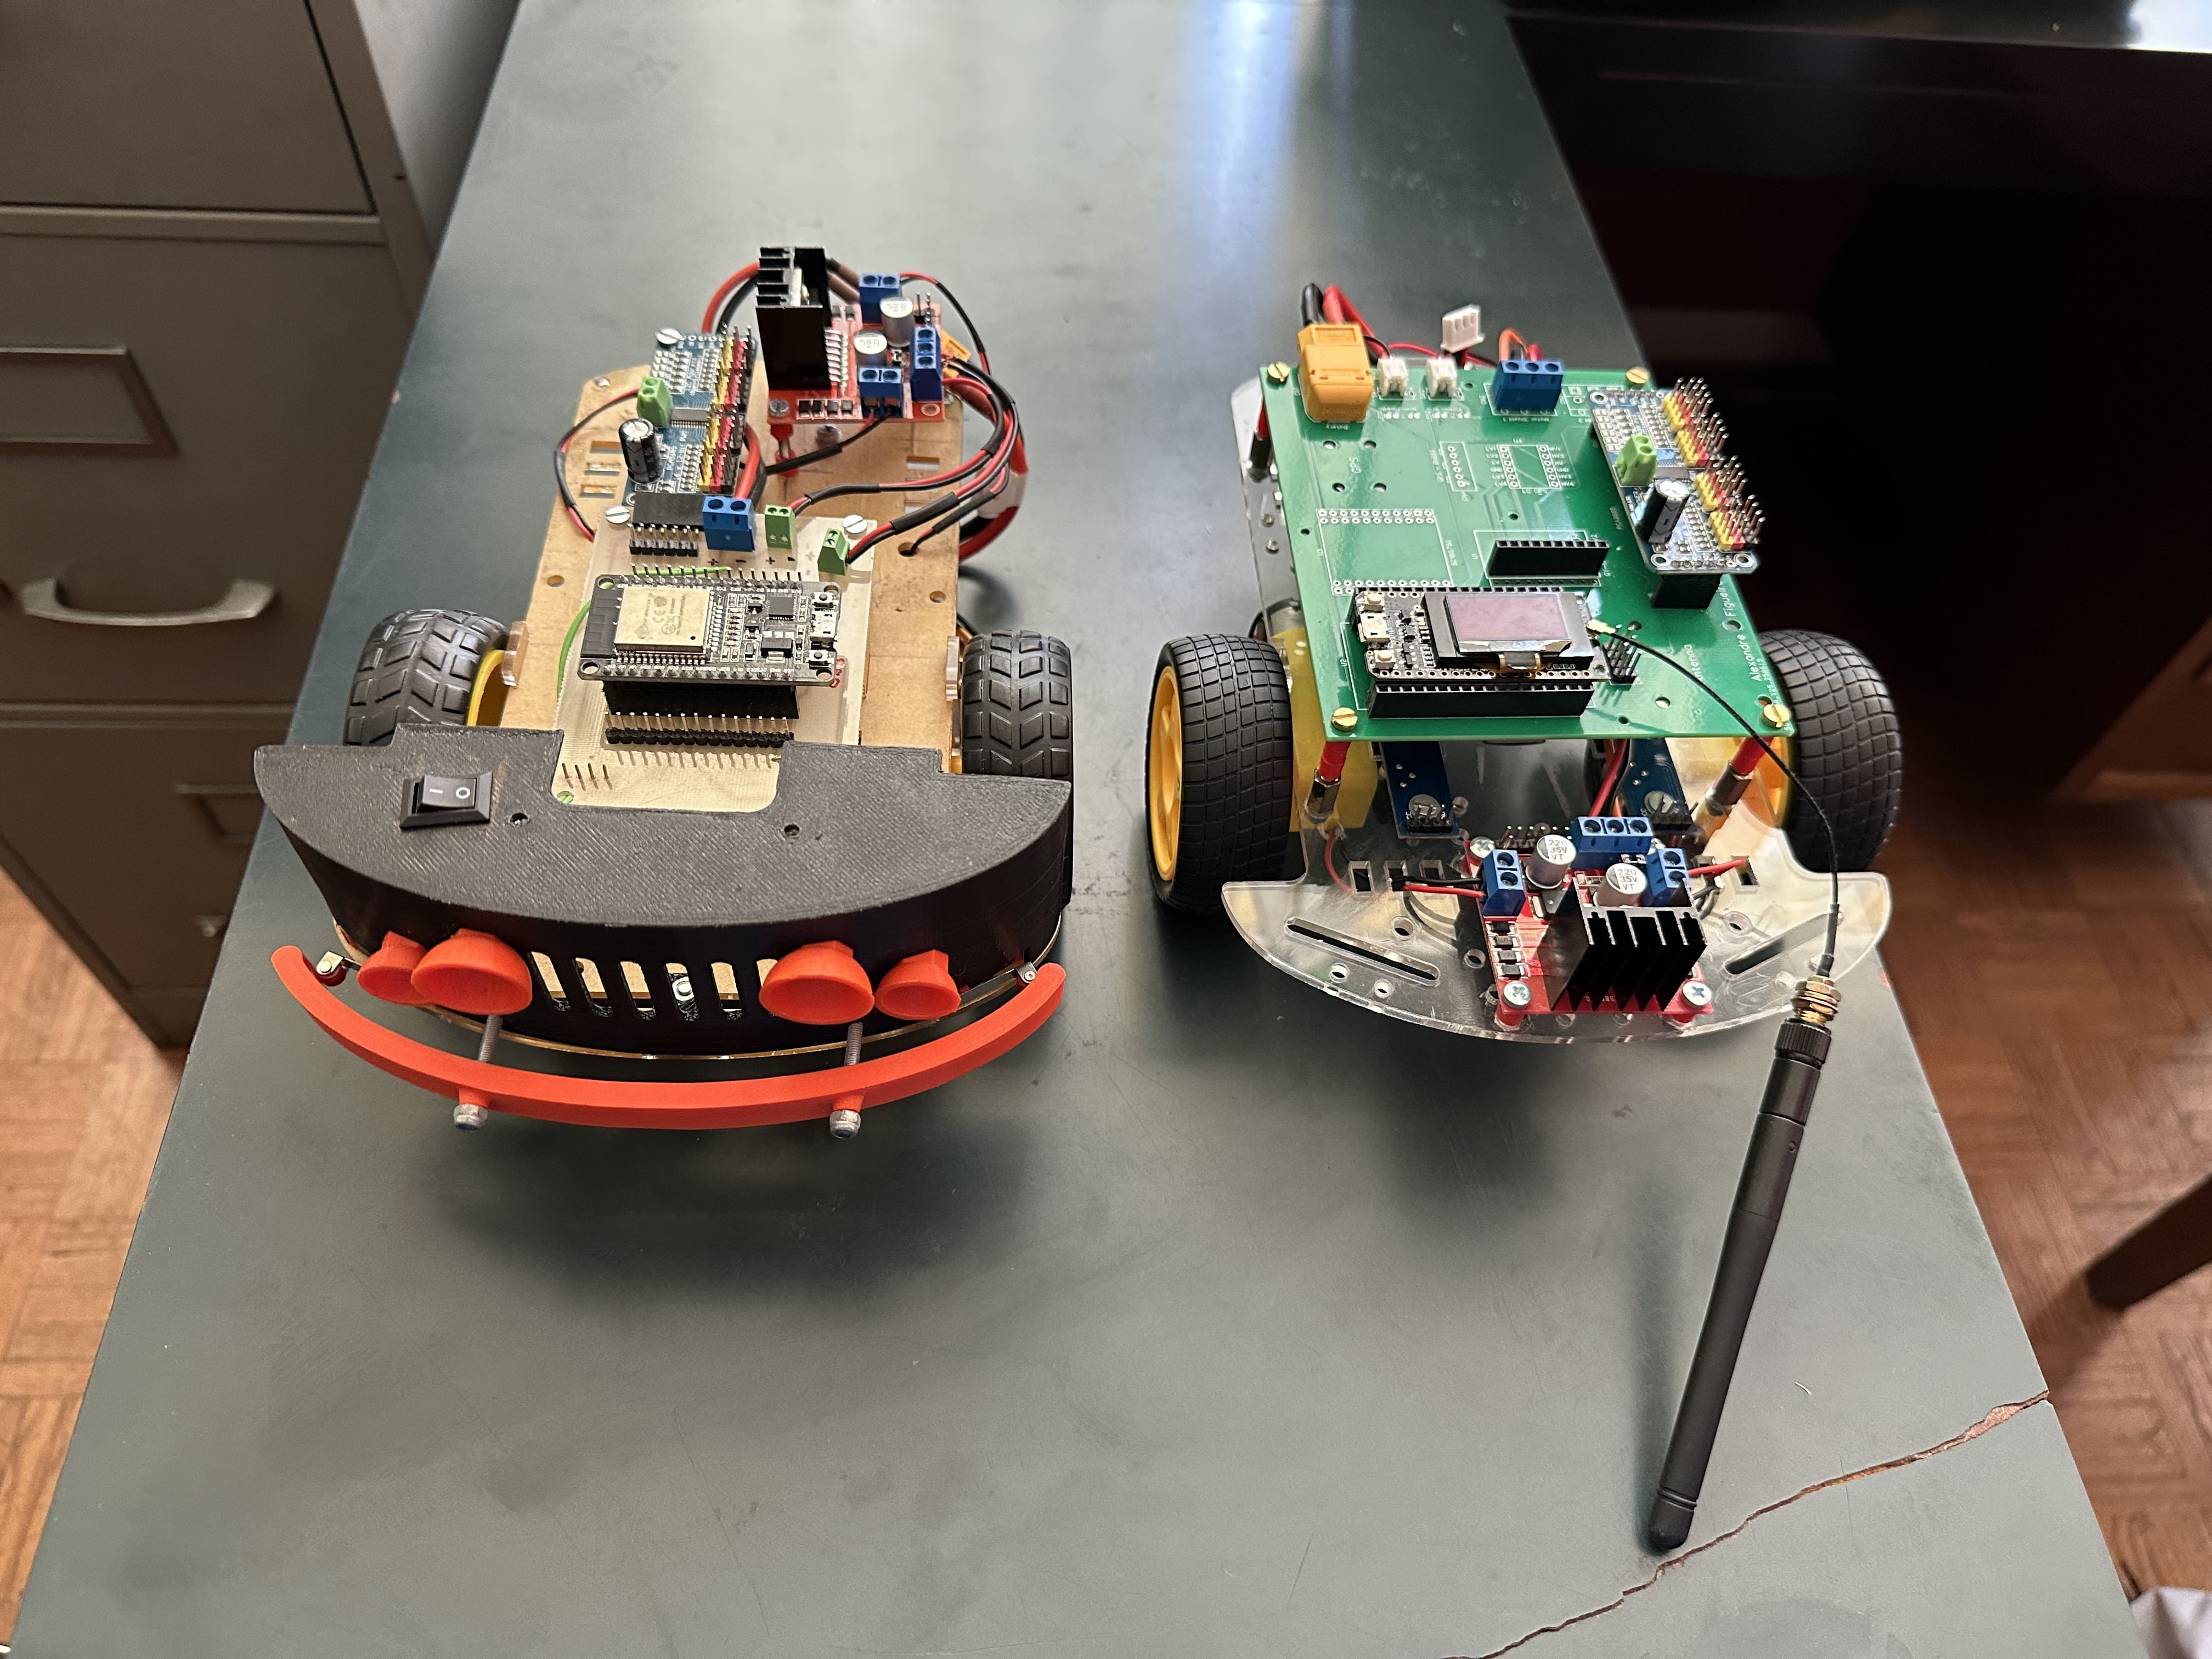
\includegraphics[width=0.5\linewidth]{figuras/robot-1-2.jpg}
    \caption{Comparação entre o robô didático original (esquerda) e a versão equipada com a \gls{pcb} desenvolvida (direita).}
    \label{fig:robot-didatico-comparacao}
\end{figure}

O vídeo apresentado na Figura \ref{fig:video-robot-didatico} ilustra o robô didático a ser controlado remotamente via \gls{lora}, com a \gls{pcb} desenvolvida a gerir os motores e a interpretar os comandos de movimento recebidos.  

\begin{figure}[H]
    \centering
    \href{https://youtu.be/Zvn3hBrHmkU}{%
        \begin{tikzpicture}
            \node[inner sep=0pt] {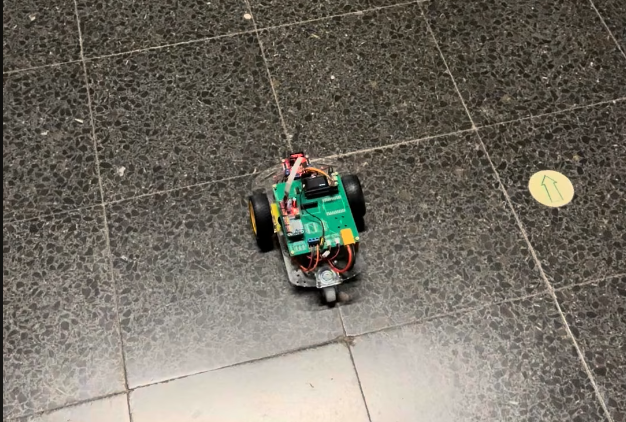
\includegraphics[width=0.5\linewidth]{didactic-robot-usb.png}};
            % Draw a red play button in the center
            \draw[fill=red, opacity=0.8] (0,0) circle [radius=0.7cm];
            \fill[white] (-0.25,0.35) -- (-0.25,-0.35) -- (0.4,0) -- cycle;
        \end{tikzpicture}%
    }
    \caption[Demonstração do robô didático em funcionamento com a \gls{pcb} desenvolvida]{Demonstração do robô didático \cite{didactic-robot-thesis} em funcionamento com a \gls{pcb} desenvolvida. (clique na imagem para abrir o vídeo no YouTube).}
    \label{fig:video-robot-didatico}
\end{figure}

Durante o ensaio foram enviados comandos em intervalos regulares de 10 segundos, alternando sequencialmente entre deslocamentos para a frente e para trás (50 cm cada), bem como rotações à direita e à esquerda, ambas com raio de 50 cm e ângulo de curvatura de 90 graus. Este teste demonstrou a correta receção, descodificação e execução dos comandos, confirmando a fiabilidade da comunicação e a consistência do sistema de controlo motor.  

Os resultados obtidos demonstram que a \gls{pcb} é plenamente capaz de controlar os motores do robô didático, assegurando a execução correta dos comandos recebidos via \gls{lora}. Esta validação inicial confirmou a funcionalidade essencial do sistema de controlo e comunicação, constituindo um passo determinante antes da integração no protótipo do \gls{usv}, ao garantir a compatibilidade entre o \emph{software} do robô didático \cite{didactic-robot-thesis} e o novo \emph{hardware}.  

A validação final do sistema ocorreu no âmbito do exercício internacional \gls{repmus25}, considerado o maior exercício mundial de robótica marítima \cite{iddportugal-repmus, sapo-repmus}. O protótipo desenvolvido foi testado no subevento \gls{rex25}, organizado pela Escola Naval \cite{escolanaval-repmus}, que visa promover a experimentação tecnológica e a cooperação em cenários operacionais simulados, no contexto das operações não tripuladas.  

Este teste constituiu um marco relevante na validação do sistema, uma vez que permitiu avaliar o desempenho do \gls{usv} em condições operacionais reais, incluindo a comunicação de longo alcance via \gls{lora} e a execução de rotas predefinidas com recurso ao \gls{gps} e ao \gls{imu}.  

A participação no \gls{rex25}, integrado no \gls{repmus25}, demonstrou a aplicabilidade prática da solução desenvolvida e reforçou o contributo da Escola Náutica e da investigação nacional no domínio dos sistemas ciberfísicos aplicados à robótica marítima. Esta validação permitiu comprovar a robustez, escalabilidade e relevância prática do sistema, consolidando o trabalho desenvolvido no âmbito desta \gls{tfm}.

Durante o processo de validação identificou-se a necessidade de complementar os testes com uma ferramenta de apoio à visualização geográfica dos \emph{waypoints}, de forma a avaliar em tempo real a coerência e a precisão das rotas definidas. Para tal, foi desenvolvida uma aplicação em \gls{html} que, recorrendo a um servidor de \emph{map tiling}, permite representar graficamente a posição geográfica de cada \emph{waypoint} no globo. Esta ferramenta revelou-se essencial para a interpretação e validação prática das trajetórias, uma vez que forneceu uma perspetiva espacial clara do percurso programado e da sua correspondência com o ambiente real.  

Para além da sua utilidade imediata na fase de testes, esta aplicação possui elevado potencial para ser expandida em trabalhos futuros, nomeadamente através da integração com sistemas de monitorização remota, planeamento dinâmico de rotas e visualização em tempo real do estado do \gls{usv}. Desta forma, poderá constituir-se como um módulo complementar para a exploração e gestão de missões autónomas em cenários operacionais complexos.  

A Figura~\ref{fig:html} apresenta uma captura de ecrã da aplicação desenvolvida, evidenciando a sua utilidade como suporte complementar à experimentação em campo.


\begin{figure}[H]
    \centering
    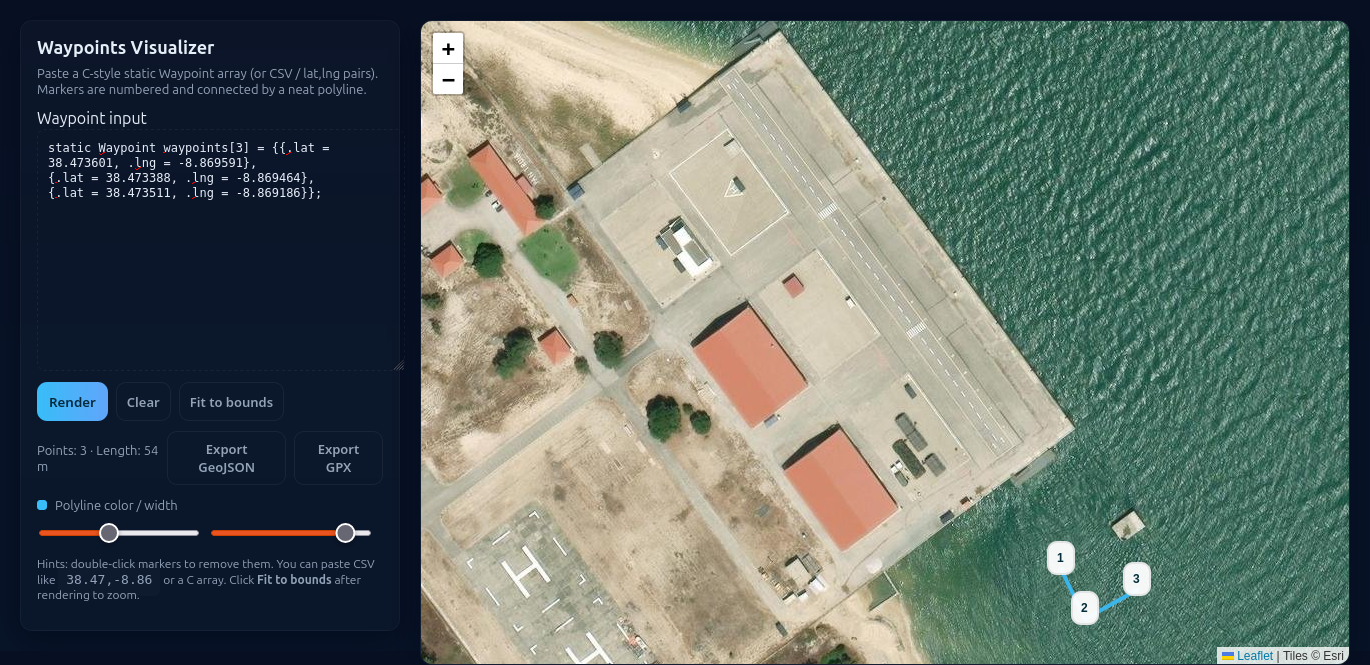
\includegraphics[width=1\linewidth]{figuras/waypoint-html.png}
    \caption{Ferramenta de visualização de \emph{waypoints}}
    \label{fig:html}
\end{figure}

A Figura \ref{fig:video-usv} apresenta um \emph{link} para um vídeo na plataforma YouTube que documenta a execução prática do \gls{usv}. O registo em video demonstra tanto as capacidades de navegação autónoma entre \emph{waypoints} pré-definidos, como o funcionamento em modo manual através de comandos remotos.  

\begin{figure}[H]
    \centering
    \href{https://youtu.be/LxEEflRIIYM}{%
        \begin{tikzpicture}
            \node[inner sep=0pt] {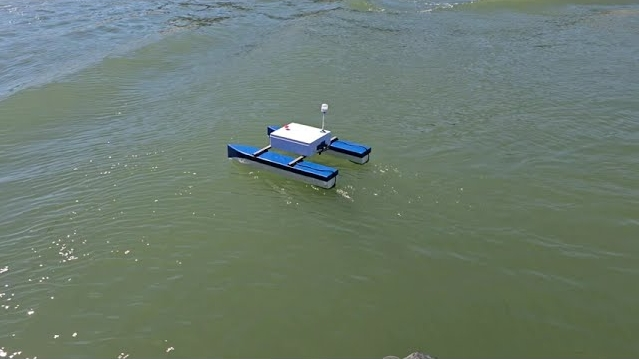
\includegraphics[width=0.5\linewidth]{thumbnail-youtube.jpg}};
            % Draw a red play button in the center
            \draw[fill=red, opacity=0.8] (0,0) circle [radius=0.7cm];
            \fill[white] (-0.25,0.35) -- (-0.25,-0.35) -- (0.4,0) -- cycle;
        \end{tikzpicture}%
    }
    \caption[Demonstração do \gls{usv} em funcionamento automático e manual]{Demonstração do \gls{usv} em funcionamento automático e manual (clique na imagem para abrir o vídeo no YouTube).}
    \label{fig:video-usv}
\end{figure}

Até aproximadamente ao minuto 1:10, é possível observar o modo autónomo de navegação, no qual o \gls{usv} percorre de forma independente uma rota estabelecida a partir de coordenadas \gls{gps}. A partir desse ponto, é evidenciado o modo de controlo manual, em que a embarcação é dirigida em tempo real por instruções transmitidas a partir da estação de controlo. Esta demonstração confirma a versatilidade do sistema, assegurando a sua capacidade de alternar de forma fiável entre modos de operação autónomo e manual.  

\section{Sumário}

A estratégia de testes adotada demonstrou-se eficaz, permitindo a deteção e resolução de problemas de forma faseada e garantindo que o sistema final apresentava fiabilidade e robustez. Os testes unitários asseguraram a operação correta de cada módulo, os ensaios de integração confirmaram a coerência da arquitetura modular, e a validação em ambiente real comprovou a aplicabilidade do protótipo em cenários operacionais complexos. Em conjunto, estes resultados confirmam o cumprimento dos objetivos estabelecidos e a viabilidade da solução proposta para o controlo autónomo de veículos de superfície não tripulados.  

\chapter{Conclusões e Trabalho Futuro}
\label{ch:conclusoesTrabalhoFuturo}

O trabalho desenvolvido permitiu conceber e validar um sistema ciberfísico modular para o controlo autónomo de embarcações do tipo \gls{usv}. O protótipo integrou propulsores \emph{brushless}, sensores de navegação (\gls{gps} e \gls{imu}), comunicação de longo alcance via \gls{lora}, bem como uma arquitetura de \emph{software} estruturada em módulos reutilizáveis. Os resultados obtidos demonstraram a viabilidade da solução em cenários reais, confirmando a robustez, a escalabilidade e o potencial de evolução do sistema.

Conclui-se que a abordagem proposta constitui uma base sólida para futuras investigações e aplicações práticas no domínio da robótica marítima com recurso a veículos de superfície não tripulados. O sistema desenvolvido provou ser capaz de operar em modo manual e automático e seguir rotas definidas por \emph{waypoints} \gls{gps}, representando um contributo relevante para a área.

No que respeita ao trabalho futuro, identificam-se várias direções de evolução. Em primeiro lugar, destaca-se a possibilidade de integração do sistema no \gls{usv}-enautica1 da Escola Superior Náutica Infante D. Henrique, permitindo validar o desempenho em cenários de maior escala. Outra vertente importante consiste na implementação de um sistema de controlo remoto manual, quer através de um comando dedicado semelhante aos utilizados em rádio controlo, quer por meio da integração com o comando desenvolvido em \cite{catamara-telecomandado}, assegurando assim a compatibilidade com plataformas operacionais. 

A expansão para guardar telemetria num cartão SD constitui igualmente um caminho relevante. Do ponto de vista do controlo, será pertinente implementar e avaliar estratégias mais avançadas, nomeadamente controladores \gls{pid}, \gls{lqr}, de controlo ótimo ou até técnicas baseadas em aprendizagem por reforço, de modo a aumentar a precisão e a robustez da navegação.

Outra linha de evolução consiste na exploração da navegação cooperativa com múltiplos \gls{usv}, o que implica a coordenação distribuída entre embarcações através de \gls{lora} ou tecnologias alternativas de comunicação em rede. Neste mesmo sentido, a integração de sensores adicionais, como GNSS multiconstelação, câmaras ou radar de baixo custo, permitirá reforçar a precisão da navegação e a resiliência do sistema em ambientes mais complexos.

A sustentabilidade energética poderá ser reforçada através da integração de painéis solares ou de sistemas híbridos de alimentação, aumentando a autonomia em missões prolongadas. Paralelamente, o desenvolvimento de uma interface de monitorização remota, acessível via aplicação web ou móvel, poderá facilitar o acompanhamento em tempo real e o registo histórico das missões realizadas. Finalmente, a realização de ensaios em condições ambientais adversas permitirá avaliar a resiliência e a fiabilidade do sistema em cenários reais de maior exigência.

Em síntese, a evolução do sistema deverá orientar-se para o aumento da autonomia, da fiabilidade e da aplicabilidade prática, consolidando o seu papel enquanto plataforma experimental e operacional para investigação e desenvolvimento na área dos veículos marítimos não tripulados \gls{usv}.


\appendix
% !TeX spellcheck = pt_PT2

\chapter{Esquemáticas \gls{pcb}}
\label{anexo:pcb}

\begin{figure}[H]
  \centering
  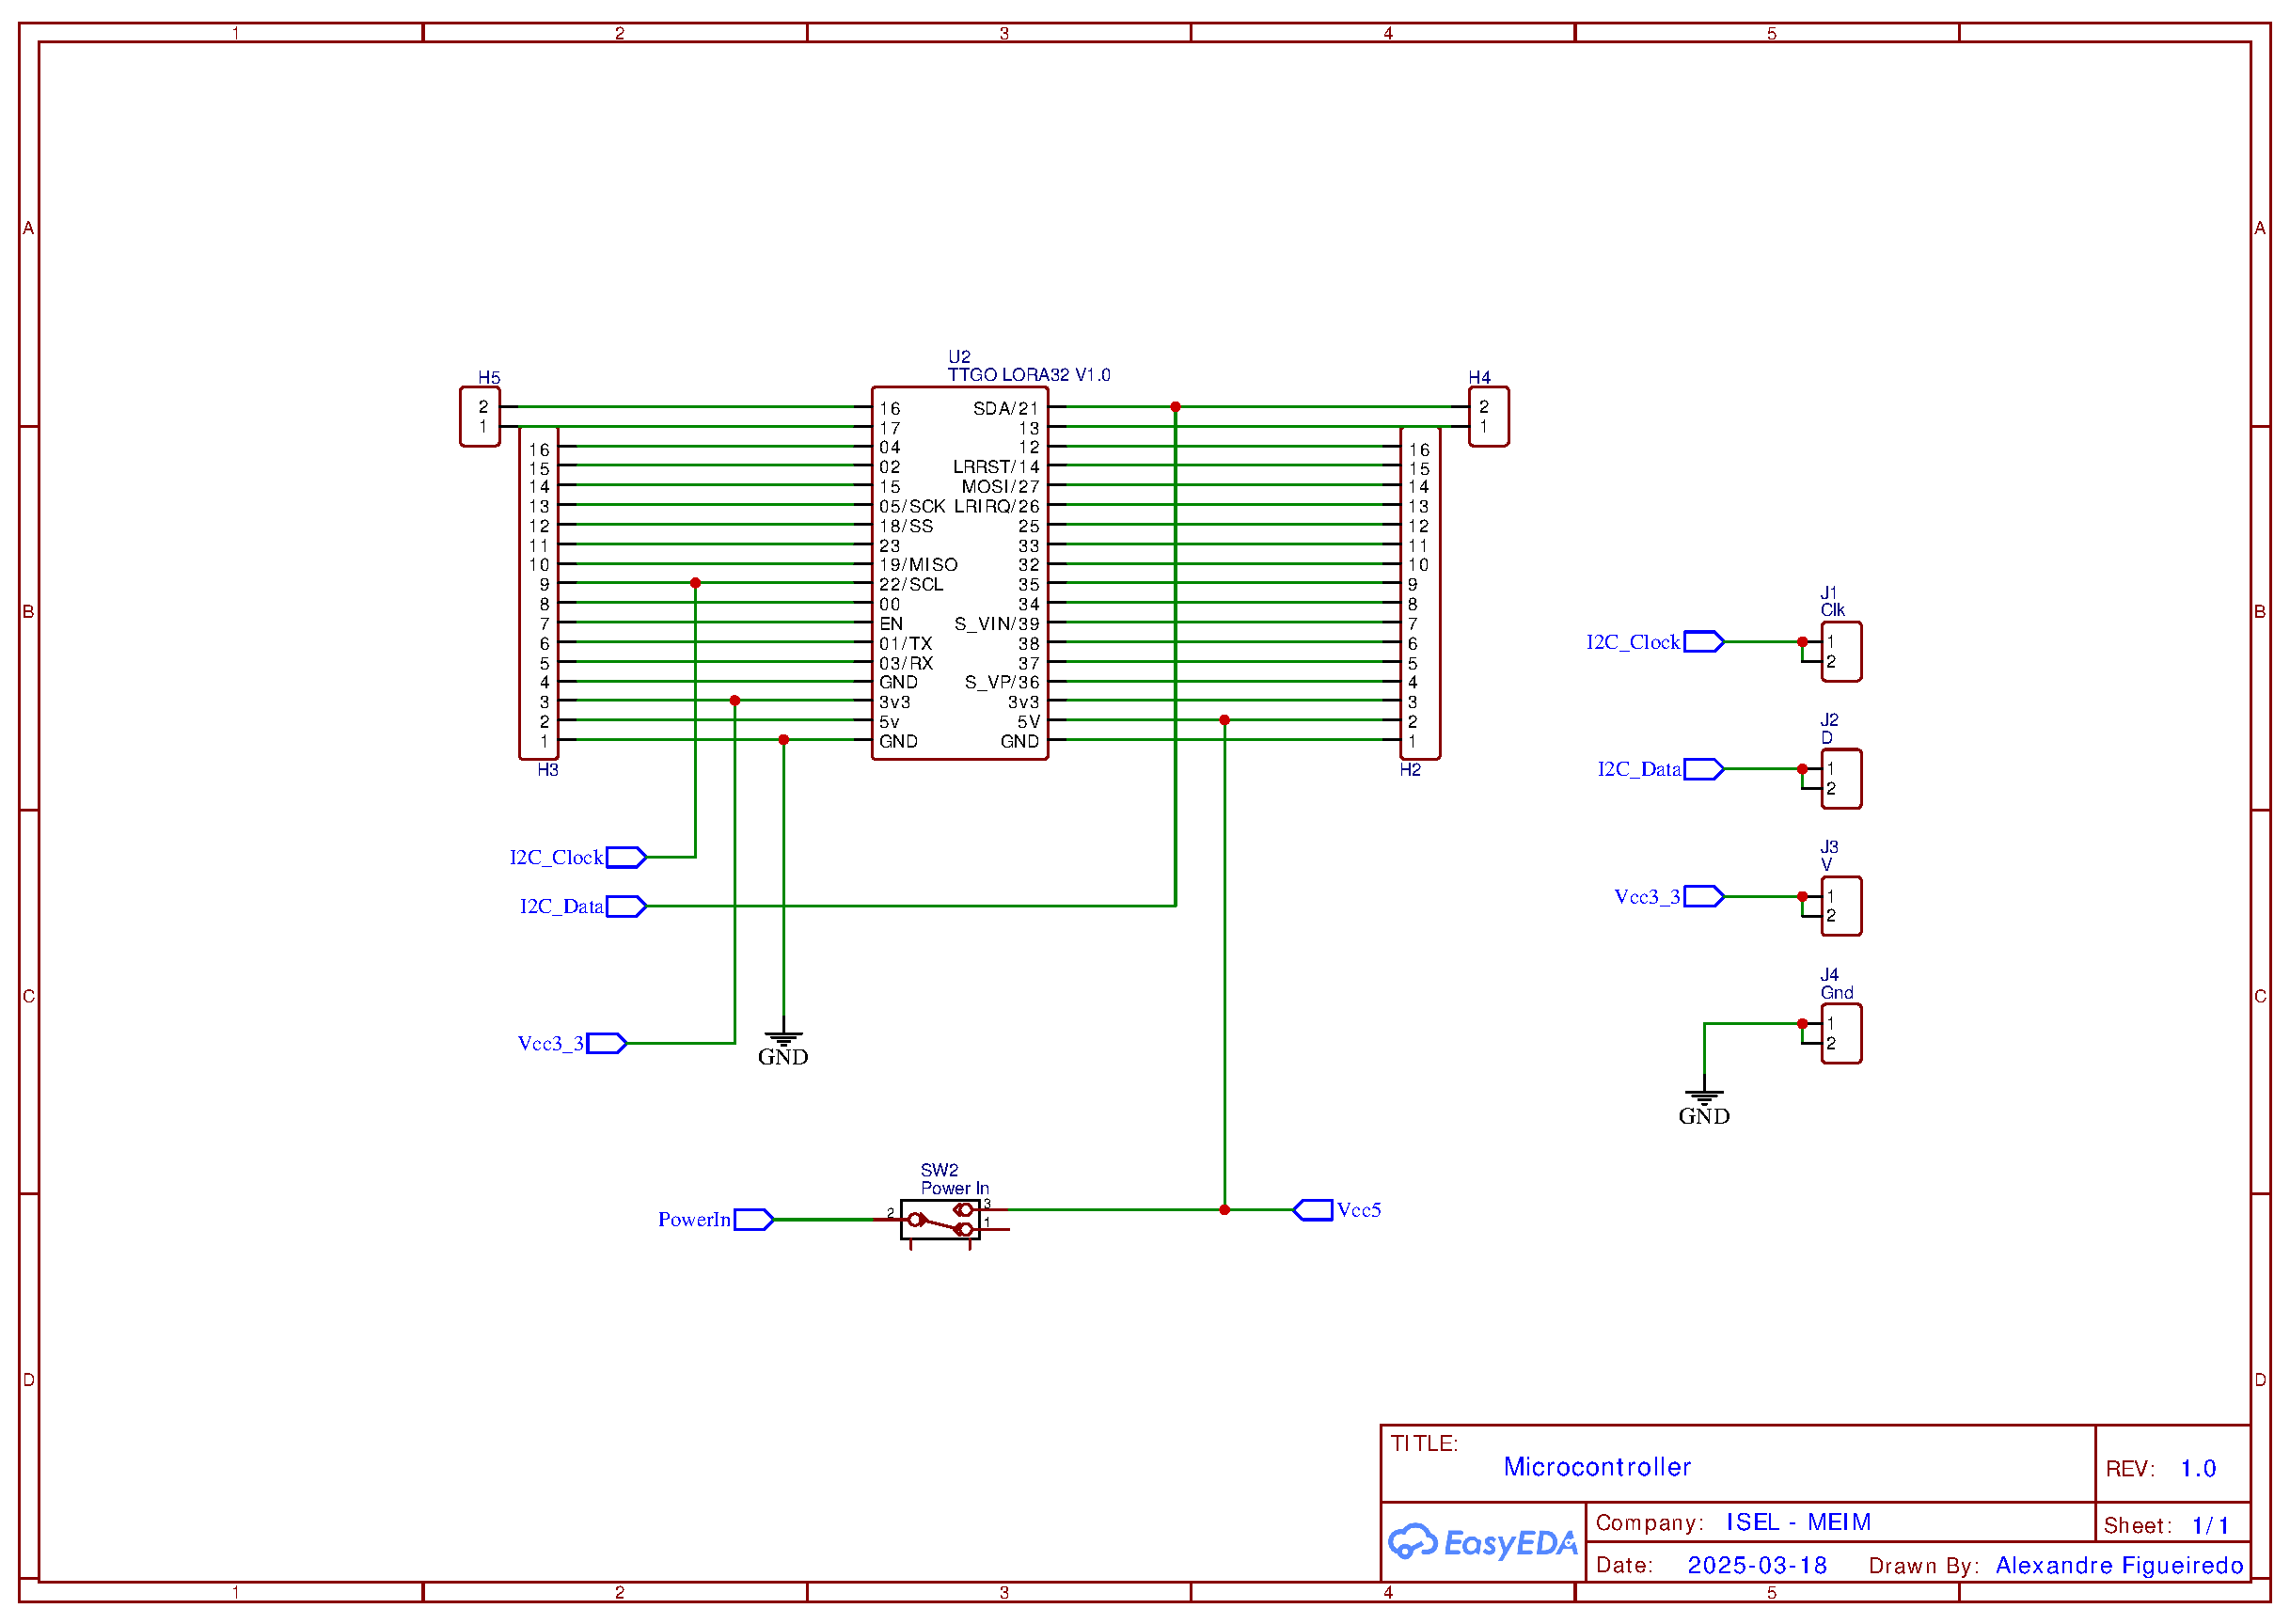
\includegraphics[page=1,width=\textwidth,height=\textheight,keepaspectratio]{anexos/esquematica.pdf}
  \caption{Esquemática do microcontrolador}
  \label{fig:esquematica-gps}
\end{figure}

\begin{figure}[H]
  \centering
  \includegraphics[page=2,width=\textwidth,height=\textheight,keepaspectratio]{anexos/esquematica.pdf}
  \caption{Esquemática dos propulsores}
  \label{fig:esquematica-props}
\end{figure}
\vspace{-0.2cm}
\begin{figure}[H]
  \centering
  \includegraphics[page=3,width=\textwidth,height=\textheight,keepaspectratio]{anexos/esquematica.pdf}
  \caption{Esquemática do \gls{imu}}}
  \label{fig:esquematica-imu}
\end{figure}

\begin{figure}[H]
  \centering
  \includegraphics[page=4,width=\textwidth,height=\textheight,keepaspectratio]{anexos/esquematica.pdf}
  \caption{Esquemática do controlo dos motores (expansor)}
  \label{fig:esquematica-expander}
\end{figure}
\vspace{-0.2cm}
\begin{figure}[H]
  \centering
  \includegraphics[page=5,width=\textwidth,height=\textheight,keepaspectratio]{anexos/esquematica.pdf}
  \caption{Esquemática do \gls{gps}}
  \label{fig:esquematica-gps}
\end{figure}

\chapter{Diagramas de classes}
\label{anexo:diagramas-de-classes}

\begin{figure}[H]
  \centering
  \resizebox{\textwidth}{!}{%
    % generated by Plantuml 1.2024.3       
\definecolor{plantucolor0000}{RGB}{255,255,255}
\definecolor{plantucolor0001}{RGB}{0,0,0}
\definecolor{plantucolor0002}{RGB}{238,238,238}
\definecolor{plantucolor0003}{RGB}{221,221,221}
\definecolor{plantucolor0004}{RGB}{204,204,204}
\definecolor{plantucolor0005}{RGB}{187,187,187}
\begin{tikzpicture}[yscale=-1
,pstyle0/.style={color=black,fill=white,line width=1.0pt}
,pstyle1/.style={color=black,line width=1.0pt}
,pstyle6/.style={color=black,fill=black,line width=1.0pt}
]
\draw[pstyle0] (794.5pt,11.602pt) -- (917.9187pt,11.602pt) arc(270:360:3.75pt)  -- (927.4187pt,36.6699pt) -- (974.5pt,36.6699pt) arc(270:360:2.5pt)  -- (977pt,349.102pt) arc(0:90:2.5pt)  -- (794.5pt,351.602pt) arc(90:180:2.5pt)  -- (792pt,14.102pt) arc(180:270:2.5pt) ;
\draw[pstyle1] (792pt,36.6699pt) -- (927.4187pt,36.6699pt);
\node at (796pt,13.602pt)[below right,color=black]{\textbf{Robot Didático}};
\draw[color=black,fill=plantucolor0002,line width=1.0pt] (13.5pt,19.602pt) -- (47.6714pt,19.602pt) arc(270:360:3.75pt)  -- (57.1714pt,44.6699pt) -- (761.5pt,44.6699pt) arc(270:360:2.5pt)  -- (764pt,117.102pt) arc(0:90:2.5pt)  -- (13.5pt,119.602pt) arc(90:180:2.5pt)  -- (11pt,22.102pt) arc(180:270:2.5pt) ;
\draw[pstyle1] (11pt,44.6699pt) -- (57.1714pt,44.6699pt);
\node at (15pt,21.602pt)[below right,color=black]{\textbf{USV}};
\draw[color=black,fill=plantucolor0003,line width=1.0pt] (404.5pt,340.602pt) -- (468.9667pt,340.602pt) arc(270:360:3.75pt)  -- (478.4667pt,365.6699pt) -- (531.5pt,365.6699pt) arc(270:360:2.5pt)  -- (534pt,473.102pt) arc(0:90:2.5pt)  -- (404.5pt,475.602pt) arc(90:180:2.5pt)  -- (402pt,343.102pt) arc(180:270:2.5pt) ;
\draw[pstyle1] (402pt,365.6699pt) -- (478.4667pt,365.6699pt);
\node at (406pt,342.602pt)[below right,color=black]{\textbf{Control}};
\draw[color=black,fill=plantucolor0004,line width=1.0pt] (601pt,428.602pt) -- (665.6727pt,428.602pt) arc(270:360:3.75pt)  -- (675.1727pt,453.6699pt) -- (722pt,453.6699pt) arc(270:360:2.5pt)  -- (724.5pt,606.102pt) arc(0:90:2.5pt)  -- (601pt,608.602pt) arc(90:180:2.5pt)  -- (598.5pt,431.102pt) arc(180:270:2.5pt) ;
\draw[pstyle1] (598.5pt,453.6699pt) -- (675.1727pt,453.6699pt);
\node at (602.5pt,430.602pt)[below right,color=black]{\textbf{Sensors}};
\draw[color=black,fill=plantucolor0005,line width=1.0pt] (181pt,303.602pt) -- (315.2991pt,303.602pt) arc(270:360:3.75pt)  -- (324.7991pt,328.6699pt) -- (325pt,328.6699pt) arc(270:360:2.5pt)  -- (327.5pt,481.102pt) arc(0:90:2.5pt)  -- (181pt,483.602pt) arc(90:180:2.5pt)  -- (178.5pt,306.102pt) arc(180:270:2.5pt) ;
\draw[pstyle1] (178.5pt,328.6699pt) -- (324.7991pt,328.6699pt);
\node at (182.5pt,305.602pt)[below right,color=black]{\textbf{Communication}};
\draw[pstyle0] (848.5pt,295.102pt) arc (180:270:5pt) -- (853.5pt,290.102pt) -- (915.8897pt,290.102pt) arc (270:360:5pt) -- (920.8897pt,295.102pt) -- (920.8897pt,330.1699pt) arc (0:90:5pt) -- (915.8897pt,335.1699pt) -- (853.5pt,335.1699pt) arc (90:180:5pt) -- (848.5pt,330.1699pt) -- cycle;
\draw[pstyle0] (860.5pt,304.6359pt) ellipse (8pt and 8pt);
\node at (860.5pt,304.6359pt)[]{\textbf{\Large C}};
\node at (871.5pt,295.102pt)[below right,color=black]{Robot};
\draw[pstyle1] (849.5pt,319.1699pt) -- (919.8897pt,319.1699pt);
\draw[pstyle1] (849.5pt,327.1699pt) -- (919.8897pt,327.1699pt);
\draw[pstyle0] (830.5pt,215.102pt) arc (180:270:5pt) -- (835.5pt,210.102pt) -- (933.7857pt,210.102pt) arc (270:360:5pt) -- (938.7857pt,215.102pt) -- (938.7857pt,250.1699pt) arc (0:90:5pt) -- (933.7857pt,255.1699pt) -- (835.5pt,255.1699pt) arc (90:180:5pt) -- (830.5pt,250.1699pt) -- cycle;
\draw[pstyle0] (842.5pt,224.6359pt) ellipse (8pt and 8pt);
\node at (842.5pt,224.6359pt)[]{\textbf{\Large C}};
\node at (853.5pt,215.102pt)[below right,color=black]{Movement};
\draw[pstyle1] (831.5pt,239.1699pt) -- (937.7857pt,239.1699pt);
\draw[pstyle1] (831.5pt,247.1699pt) -- (937.7857pt,247.1699pt);
\draw[pstyle0] (847.5pt,135.102pt) arc (180:270:5pt) -- (852.5pt,130.102pt) -- (916.7244pt,130.102pt) arc (270:360:5pt) -- (921.7244pt,135.102pt) -- (921.7244pt,170.1699pt) arc (0:90:5pt) -- (916.7244pt,175.1699pt) -- (852.5pt,175.1699pt) arc (90:180:5pt) -- (847.5pt,170.1699pt) -- cycle;
\draw[pstyle0] (859.5pt,144.6359pt) ellipse (8pt and 8pt);
\node at (859.5pt,144.6359pt)[]{\textbf{\Large C}};
\node at (870.5pt,135.102pt)[below right,color=black]{Motor};
\draw[pstyle1] (848.5pt,159.1699pt) -- (920.7244pt,159.1699pt);
\draw[pstyle1] (848.5pt,167.1699pt) -- (920.7244pt,167.1699pt);
\draw[pstyle0] (808pt,55.102pt) arc (180:270:5pt) -- (813pt,50.102pt) -- (956.4972pt,50.102pt) arc (270:360:5pt) -- (961.4972pt,55.102pt) -- (961.4972pt,90.1699pt) arc (0:90:5pt) -- (956.4972pt,95.1699pt) -- (813pt,95.1699pt) arc (90:180:5pt) -- (808pt,90.1699pt) -- cycle;
\draw[pstyle0] (820pt,64.6359pt) ellipse (8pt and 8pt);
\node at (820pt,64.6359pt)[]{\textbf{\Large C}};
\node at (831pt,55.102pt)[below right,color=black]{MotorController};
\draw[pstyle1] (809pt,79.1699pt) -- (960.4972pt,79.1699pt);
\draw[pstyle1] (809pt,87.1699pt) -- (960.4972pt,87.1699pt);
\draw[pstyle0] (27pt,63.102pt) arc (180:270:5pt) -- (32pt,58.102pt) -- (79.2148pt,58.102pt) arc (270:360:5pt) -- (84.2148pt,63.102pt) -- (84.2148pt,98.1699pt) arc (0:90:5pt) -- (79.2148pt,103.1699pt) -- (32pt,103.1699pt) arc (90:180:5pt) -- (27pt,98.1699pt) -- cycle;
\draw[pstyle0] (39pt,72.6359pt) ellipse (8pt and 8pt);
\node at (39pt,72.6359pt)[]{\textbf{\Large C}};
\node at (50pt,63.102pt)[below right,color=black]{USV};
\draw[pstyle1] (28pt,87.1699pt) -- (83.2148pt,87.1699pt);
\draw[pstyle1] (28pt,95.1699pt) -- (83.2148pt,95.1699pt);
\draw[pstyle0] (144pt,63.102pt) arc (180:270:5pt) -- (149pt,58.102pt) -- (355.9463pt,58.102pt) arc (270:360:5pt) -- (360.9463pt,63.102pt) -- (360.9463pt,98.1699pt) arc (0:90:5pt) -- (355.9463pt,103.1699pt) -- (149pt,103.1699pt) arc (90:180:5pt) -- (144pt,98.1699pt) -- cycle;
\draw[pstyle0] (156pt,72.6359pt) ellipse (8pt and 8pt);
\node at (156pt,72.6359pt)[]{\textbf{\Large C}};
\node at (167pt,63.102pt)[below right,color=black]{MovementTwoThrusters};
\draw[pstyle1] (145pt,87.1699pt) -- (359.9463pt,87.1699pt);
\draw[pstyle1] (145pt,95.1699pt) -- (359.9463pt,95.1699pt);
\draw[pstyle0] (421pt,63.102pt) arc (180:270:5pt) -- (426pt,58.102pt) -- (509.7492pt,58.102pt) arc (270:360:5pt) -- (514.7492pt,63.102pt) -- (514.7492pt,98.1699pt) arc (0:90:5pt) -- (509.7492pt,103.1699pt) -- (426pt,103.1699pt) arc (90:180:5pt) -- (421pt,98.1699pt) -- cycle;
\draw[pstyle0] (433pt,72.6359pt) ellipse (8pt and 8pt);
\node at (433pt,72.6359pt)[]{\textbf{\Large C}};
\node at (444pt,63.102pt)[below right,color=black]{Thruster};
\draw[pstyle1] (422pt,87.1699pt) -- (513.7492pt,87.1699pt);
\draw[pstyle1] (422pt,95.1699pt) -- (513.7492pt,95.1699pt);
\draw[pstyle0] (575pt,63.102pt) arc (180:270:5pt) -- (580pt,58.102pt) -- (743.0142pt,58.102pt) arc (270:360:5pt) -- (748.0142pt,63.102pt) -- (748.0142pt,98.1699pt) arc (0:90:5pt) -- (743.0142pt,103.1699pt) -- (580pt,103.1699pt) arc (90:180:5pt) -- (575pt,98.1699pt) -- cycle;
\draw[pstyle0] (587pt,72.6359pt) ellipse (8pt and 8pt);
\node at (587pt,72.6359pt)[]{\textbf{\Large S}};
\node at (598pt,63.102pt)[below right,color=black]{ThrusterController};
\draw[pstyle1] (576pt,87.1699pt) -- (747.0142pt,87.1699pt);
\draw[pstyle1] (576pt,95.1699pt) -- (747.0142pt,95.1699pt);
\draw[pstyle0] (426pt,392.102pt) arc (180:270:5pt) -- (431pt,387.102pt) -- (505.32pt,387.102pt) arc (270:360:5pt) -- (510.32pt,392.102pt) -- (510.32pt,427.1699pt) arc (0:90:5pt) -- (505.32pt,432.1699pt) -- (431pt,432.1699pt) arc (90:180:5pt) -- (426pt,427.1699pt) -- cycle;
\draw[pstyle0] (438pt,401.6359pt) ellipse (8pt and 8pt);
\node at (438pt,401.6359pt)[]{\textbf{\Large C}};
\node at (449pt,392.102pt)[below right,color=black]{Control};
\draw[pstyle1] (427pt,416.1699pt) -- (509.32pt,416.1699pt);
\draw[pstyle1] (427pt,424.1699pt) -- (509.32pt,424.1699pt);
\draw[pstyle0] (615.5pt,472.102pt) arc (180:270:5pt) -- (620.5pt,467.102pt) -- (702.093pt,467.102pt) arc (270:360:5pt) -- (707.093pt,472.102pt) -- (707.093pt,507.1699pt) arc (0:90:5pt) -- (702.093pt,512.1699pt) -- (620.5pt,512.1699pt) arc (90:180:5pt) -- (615.5pt,507.1699pt) -- cycle;
\draw[pstyle0] (627.5pt,481.6359pt) ellipse (8pt and 8pt);
\node at (627.5pt,481.6359pt)[]{\textbf{\Large C}};
\node at (638.5pt,472.102pt)[below right,color=black]{GPSData};
\draw[pstyle1] (616.5pt,496.1699pt) -- (706.093pt,496.1699pt);
\draw[pstyle1] (616.5pt,504.1699pt) -- (706.093pt,504.1699pt);
\draw[pstyle0] (614.5pt,552.102pt) arc (180:270:5pt) -- (619.5pt,547.102pt) -- (703.2492pt,547.102pt) arc (270:360:5pt) -- (708.2492pt,552.102pt) -- (708.2492pt,587.1699pt) arc (0:90:5pt) -- (703.2492pt,592.1699pt) -- (619.5pt,592.1699pt) arc (90:180:5pt) -- (614.5pt,587.1699pt) -- cycle;
\draw[pstyle0] (626.5pt,561.6359pt) ellipse (8pt and 8pt);
\node at (626.5pt,561.6359pt)[]{\textbf{\Large C}};
\node at (637.5pt,552.102pt)[below right,color=black]{IMUData};
\draw[pstyle1] (615.5pt,576.1699pt) -- (707.2492pt,576.1699pt);
\draw[pstyle1] (615.5pt,584.1699pt) -- (707.2492pt,584.1699pt);
\draw[pstyle0] (225pt,347.102pt) arc (180:270:5pt) -- (230pt,342.102pt) -- (275.04pt,342.102pt) arc (270:360:5pt) -- (280.04pt,347.102pt) -- (280.04pt,382.1699pt) arc (0:90:5pt) -- (275.04pt,387.1699pt) -- (230pt,387.1699pt) arc (90:180:5pt) -- (225pt,382.1699pt) -- cycle;
\draw[pstyle0] (237pt,356.6359pt) ellipse (8pt and 8pt);
\node at (237pt,356.6359pt)[]{\textbf{\Large C}};
\node at (248pt,347.102pt)[below right,color=black]{Led};
\draw[pstyle1] (226pt,371.1699pt) -- (279.04pt,371.1699pt);
\draw[pstyle1] (226pt,379.1699pt) -- (279.04pt,379.1699pt);
\draw[pstyle0] (219.5pt,427.102pt) arc (180:270:5pt) -- (224.5pt,422.102pt) -- (280.3588pt,422.102pt) arc (270:360:5pt) -- (285.3588pt,427.102pt) -- (285.3588pt,462.1699pt) arc (0:90:5pt) -- (280.3588pt,467.1699pt) -- (224.5pt,467.1699pt) arc (90:180:5pt) -- (219.5pt,462.1699pt) -- cycle;
\draw[pstyle0] (231.5pt,436.6359pt) ellipse (8pt and 8pt);
\node at (231.5pt,436.6359pt)[]{\textbf{\Large C}};
\node at (242.5pt,427.102pt)[below right,color=black]{LoRa};
\draw[pstyle1] (220.5pt,451.1699pt) -- (284.3588pt,451.1699pt);
\draw[pstyle1] (220.5pt,459.1699pt) -- (284.3588pt,459.1699pt);
\draw[pstyle1] (76pt,103.272pt) ..controls (76pt,161.642pt) and (76pt,312.602pt) .. (76pt,312.602pt) ..controls (76pt,312.602pt) and (673.56pt,312.602pt) .. (830.45pt,312.602pt);
\draw[pstyle1] (848.45pt,312.602pt) -- (830.45pt,306.602pt) -- (830.45pt,318.602pt) -- (848.45pt,312.602pt) -- cycle;
\draw[pstyle1] (324pt,103.362pt) ..controls (324pt,145.762pt) and (324pt,232.602pt) .. (324pt,232.602pt) ..controls (324pt,232.602pt) and (671.58pt,232.602pt) .. (812.25pt,232.602pt);
\draw[pstyle1] (830.25pt,232.602pt) -- (812.25pt,226.602pt) -- (812.25pt,238.602pt) -- (830.25pt,232.602pt) -- cycle;
\draw[pstyle1] (468pt,103.382pt) ..controls (468pt,124.482pt) and (468pt,152.602pt) .. (468pt,152.602pt) ..controls (468pt,152.602pt) and (726.94pt,152.602pt) .. (829.17pt,152.602pt);
\draw[pstyle1] (847.17pt,152.602pt) -- (829.17pt,146.602pt) -- (829.17pt,158.602pt) -- (847.17pt,152.602pt) -- cycle;
\draw[pstyle1] (748.04pt,76.602pt) ..controls (767.75pt,76.602pt) and (770.56pt,76.602pt) .. (789.82pt,76.602pt);
\draw[pstyle1] (807.82pt,76.602pt) -- (789.82pt,70.602pt) -- (789.82pt,82.602pt) -- (807.82pt,76.602pt) -- cycle;
\draw[pstyle1] (96.15pt,80.602pt) ..controls (112.37pt,80.602pt) and (121.79pt,80.602pt) .. (143.91pt,80.602pt);
\draw[pstyle1] (84.15pt,80.602pt) -- (90.15pt,84.602pt) -- (96.15pt,80.602pt) -- (90.15pt,76.602pt) -- (84.15pt,80.602pt) -- cycle;
\draw[pstyle1] (52pt,115.382pt) ..controls (52pt,198.392pt) and (52pt,467.852pt) .. (52pt,467.852pt) ..controls (52pt,467.852pt) and (152.775pt,467.852pt) .. (255.125pt,467.852pt) ..controls (306.3pt,467.852pt) and (357.8688pt,467.852pt) .. (397.4313pt,467.852pt) ..controls (398.6676pt,467.852pt) and (399.8922pt,467.852pt) .. (401.1047pt,467.852pt);
\draw[pstyle6] (52pt,103.382pt) -- (48pt,109.382pt) -- (52pt,115.382pt) -- (56pt,109.382pt) -- (52pt,103.382pt) -- cycle;
\draw[pstyle1] (60pt,115.372pt) ..controls (60pt,195.062pt) and (60pt,444.602pt) .. (60pt,444.602pt) ..controls (60pt,444.602pt) and (164.37pt,444.602pt) .. (219.41pt,444.602pt);
\draw[pstyle6] (60pt,103.372pt) -- (56pt,109.372pt) -- (60pt,115.372pt) -- (64pt,109.372pt) -- (60pt,103.372pt) -- cycle;
\draw[pstyle1] (68pt,115.362pt) ..controls (68pt,182.752pt) and (68pt,364.602pt) .. (68pt,364.602pt) ..controls (68pt,364.602pt) and (173.41pt,364.602pt) .. (224.88pt,364.602pt);
\draw[pstyle1] (68pt,103.362pt) -- (64pt,109.362pt) -- (68pt,115.362pt) -- (72pt,109.362pt) -- (68pt,103.362pt) -- cycle;
\draw[pstyle1] (44pt,103.212pt) ..controls (44pt,189.112pt) and (44pt,490.352pt) .. (44pt,490.352pt) ..controls (44pt,490.352pt) and (465.98pt,490.352pt) .. (609.34pt,490.352pt);
\draw[pstyle6] (615.34pt,490.352pt) -- (606.34pt,486.352pt) -- (610.34pt,490.352pt) -- (606.34pt,494.352pt) -- (615.34pt,490.352pt) -- cycle;
\draw[pstyle1] (36pt,103.222pt) ..controls (36pt,200.352pt) and (36pt,577.102pt) .. (36pt,577.102pt) ..controls (36pt,577.102pt) and (463.02pt,577.102pt) .. (608.49pt,577.102pt);
\draw[pstyle6] (614.49pt,577.102pt) -- (605.49pt,573.102pt) -- (609.49pt,577.102pt) -- (605.49pt,581.102pt) -- (614.49pt,577.102pt) -- cycle;
\draw[pstyle1] (534.674pt,467.852pt) ..controls (534.9091pt,467.852pt) and (535.1444pt,467.852pt) .. (535.3801pt,467.852pt) ..controls (539.1499pt,467.852pt) and (542.9855pt,467.852pt) .. (546.8607pt,467.852pt) ..controls (554.6111pt,467.852pt) and (562.5202pt,467.852pt) .. (570.3795pt,467.852pt) ..controls (586.0981pt,467.852pt) and (595.6175pt,467.852pt) .. (609.27pt,467.852pt);
\draw[pstyle6] (615.27pt,467.852pt) -- (606.27pt,463.852pt) -- (610.27pt,467.852pt) -- (606.27pt,471.852pt) -- (615.27pt,467.852pt) -- cycle;
\draw[pstyle1] (468pt,475.7586pt) ..controls (468pt,476.1757pt) and (468pt,476.6062pt) .. (468pt,477.0494pt) ..controls (468pt,477.9359pt) and (468pt,478.8733pt) .. (468pt,479.8568pt) ..controls (468pt,481.8238pt) and (468pt,483.9748pt) .. (468pt,486.27pt) ..controls (468pt,495.4504pt) and (468pt,506.9364pt) .. (468pt,518.1707pt) ..controls (468pt,540.6395pt) and (468pt,562.102pt) .. (468pt,562.102pt) ..controls (468pt,562.102pt) and (550.88pt,562.102pt) .. (608.16pt,562.102pt);
\draw[pstyle6] (614.16pt,562.102pt) -- (605.16pt,558.102pt) -- (609.16pt,562.102pt) -- (605.16pt,566.102pt) -- (614.16pt,562.102pt) -- cycle;
\draw[pstyle1] (297.7pt,466.852pt) ..controls (327.45pt,466.852pt) and (360.0775pt,466.852pt) .. (397.73pt,466.852pt) ..controls (398.9066pt,466.852pt) and (400.0765pt,466.852pt) .. (401.2388pt,466.852pt);
\draw[pstyle1] (285.7pt,466.852pt) -- (291.7pt,470.852pt) -- (297.7pt,466.852pt) -- (291.7pt,462.852pt) -- (285.7pt,466.852pt) -- cycle;
\draw[pstyle1] (527.34pt,80.602pt) ..controls (545.24pt,80.602pt) and (554.22pt,80.602pt) .. (574.62pt,80.602pt);
\draw[pstyle6] (515.34pt,80.602pt) -- (521.34pt,84.602pt) -- (527.34pt,80.602pt) -- (521.34pt,76.602pt) -- (515.34pt,80.602pt) -- cycle;
\draw[pstyle1] (373.2pt,80.602pt) ..controls (394.22pt,80.602pt) and (403.2pt,80.602pt) .. (420.93pt,80.602pt);
\draw[pstyle6] (361.2pt,80.602pt) -- (367.2pt,84.602pt) -- (373.2pt,80.602pt) -- (367.2pt,76.602pt) -- (361.2pt,80.602pt) -- cycle;
\end{tikzpicture}
%
  }
  \caption{Diagrama de classes - Versão simplificada}
  \label{fig:minimalista_v3}
\end{figure}

\begin{figure}[H]
  \centering
  \resizebox{\textwidth}{!}{%
    % generated by Plantuml 1.2024.3       
\definecolor{plantucolor0000}{RGB}{238,238,238}
\definecolor{plantucolor0001}{RGB}{0,0,0}
\definecolor{plantucolor0002}{RGB}{255,255,255}
\definecolor{plantucolor0003}{RGB}{221,221,221}
\begin{tikzpicture}[yscale=-1
,pstyle1/.style={color=black,line width=1.0pt}
,pstyle2/.style={color=black,fill=white,line width=1.0pt}
,pstyle4/.style={color=black,fill=black,line width=1.0pt}
]
\draw[color=black,fill=plantucolor0000,line width=1.0pt] (13.5pt,11.602pt) -- (47.6714pt,11.602pt) arc(270:360:3.75pt)  -- (57.1714pt,36.6699pt) -- (992pt,36.6699pt) arc(270:360:2.5pt)  -- (994.5pt,995.102pt) arc(0:90:2.5pt)  -- (13.5pt,997.602pt) arc(90:180:2.5pt)  -- (11pt,14.102pt) arc(180:270:2.5pt) ;
\draw[pstyle1] (11pt,36.6699pt) -- (57.1714pt,36.6699pt);
\node at (15pt,13.602pt)[below right,color=black]{\textbf{USV}};
\draw[pstyle2] (313pt,873.602pt) -- (377.4667pt,873.602pt) arc(270:360:3.75pt)  -- (386.9667pt,898.6699pt) -- (424pt,898.6699pt) arc(270:360:2.5pt)  -- (426.5pt,971.102pt) arc(0:90:2.5pt)  -- (313pt,973.602pt) arc(90:180:2.5pt)  -- (310.5pt,876.102pt) arc(180:270:2.5pt) ;
\draw[pstyle1] (310.5pt,898.6699pt) -- (386.9667pt,898.6699pt);
\node at (314.5pt,875.602pt)[below right,color=black]{\textbf{Control}};
\draw[pstyle2] (300.5pt,669.602pt) -- (434.7991pt,669.602pt) arc(270:360:3.75pt)  -- (444.2991pt,694.6699pt) -- (697.5pt,694.6699pt) arc(270:360:2.5pt)  -- (700pt,847.102pt) arc(0:90:2.5pt)  -- (300.5pt,849.602pt) arc(90:180:2.5pt)  -- (298pt,672.102pt) arc(180:270:2.5pt) ;
\draw[pstyle1] (298pt,694.6699pt) -- (444.2991pt,694.6699pt);
\node at (302pt,671.602pt)[below right,color=black]{\textbf{Communication}};
\draw[pstyle2] (55pt,421.602pt) -- (88.1714pt,421.602pt) arc(270:360:3.75pt)  -- (97.6714pt,446.6699pt) -- (428pt,446.6699pt) arc(270:360:2.5pt)  -- (430.5pt,519.102pt) arc(0:90:2.5pt)  -- (55pt,521.602pt) arc(90:180:2.5pt)  -- (52.5pt,424.102pt) arc(180:270:2.5pt) ;
\draw[pstyle1] (52.5pt,446.6699pt) -- (97.6714pt,446.6699pt);
\node at (56.5pt,423.602pt)[below right,color=black]{\textbf{GPS}};
\draw[pstyle2] (37.5pt,57.602pt) -- (72.1966pt,57.602pt) arc(270:360:3.75pt)  -- (81.6966pt,82.6699pt) -- (707pt,82.6699pt) arc(270:360:2.5pt)  -- (709.5pt,395.102pt) arc(0:90:2.5pt)  -- (37.5pt,397.602pt) arc(90:180:2.5pt)  -- (35pt,60.102pt) arc(180:270:2.5pt) ;
\draw[pstyle1] (35pt,82.6699pt) -- (81.6966pt,82.6699pt);
\node at (39pt,59.602pt)[below right,color=black]{\textbf{IMU}};
\draw[pstyle2] (83.5pt,545.602pt) -- (117.6714pt,545.602pt) arc(270:360:3.75pt)  -- (127.1714pt,570.6699pt) -- (968pt,570.6699pt) arc(270:360:2.5pt)  -- (970.5pt,643.102pt) arc(0:90:2.5pt)  -- (83.5pt,645.602pt) arc(90:180:2.5pt)  -- (81pt,548.102pt) arc(180:270:2.5pt) ;
\draw[pstyle1] (81pt,570.6699pt) -- (127.1714pt,570.6699pt);
\node at (85pt,547.602pt)[below right,color=black]{\textbf{USV}};
\draw[color=black,fill=plantucolor0003,line width=1.0pt] (515.5pt,1029.602pt) -- (627.6167pt,1029.602pt) arc(270:360:3.75pt)  -- (637.1167pt,1054.6699pt) -- (1286.5pt,1054.6699pt) arc(270:360:2.5pt)  -- (1289pt,1311.102pt) arc(0:90:2.5pt)  -- (515.5pt,1313.602pt) arc(90:180:2.5pt)  -- (513pt,1032.102pt) arc(180:270:2.5pt) ;
\draw[pstyle1] (513pt,1054.6699pt) -- (637.1167pt,1054.6699pt);
\node at (517pt,1031.602pt)[below right,color=black]{\textbf{Protobuf:USV}};
\draw[pstyle2] (326.5pt,917.102pt) arc (180:270:5pt) -- (331.5pt,912.102pt) -- (405.82pt,912.102pt) arc (270:360:5pt) -- (410.82pt,917.102pt) -- (410.82pt,952.1699pt) arc (0:90:5pt) -- (405.82pt,957.1699pt) -- (331.5pt,957.1699pt) arc (90:180:5pt) -- (326.5pt,952.1699pt) -- cycle;
\draw[pstyle2] (338.5pt,926.6359pt) ellipse (8pt and 8pt);
\node at (338.5pt,926.6359pt)[]{\textbf{\Large C}};
\node at (349.5pt,917.102pt)[below right,color=black]{Control};
\draw[pstyle1] (327.5pt,941.1699pt) -- (409.82pt,941.1699pt);
\draw[pstyle1] (327.5pt,949.1699pt) -- (409.82pt,949.1699pt);
\draw[pstyle2] (341pt,713.102pt) arc (180:270:5pt) -- (346pt,708.102pt) -- (391.04pt,708.102pt) arc (270:360:5pt) -- (396.04pt,713.102pt) -- (396.04pt,748.1699pt) arc (0:90:5pt) -- (391.04pt,753.1699pt) -- (346pt,753.1699pt) arc (90:180:5pt) -- (341pt,748.1699pt) -- cycle;
\draw[pstyle2] (353pt,722.6359pt) ellipse (8pt and 8pt);
\node at (353pt,722.6359pt)[]{\textbf{\Large C}};
\node at (364pt,713.102pt)[below right,color=black]{Led};
\draw[pstyle1] (342pt,737.1699pt) -- (395.04pt,737.1699pt);
\draw[pstyle1] (342pt,745.1699pt) -- (395.04pt,745.1699pt);
\draw[pstyle2] (564pt,713.102pt) arc (180:270:5pt) -- (569pt,708.102pt) -- (679.237pt,708.102pt) arc (270:360:5pt) -- (684.237pt,713.102pt) -- (684.237pt,748.1699pt) arc (0:90:5pt) -- (679.237pt,753.1699pt) -- (569pt,753.1699pt) arc (90:180:5pt) -- (564pt,748.1699pt) -- cycle;
\draw[pstyle2] (576pt,722.6359pt) ellipse (8pt and 8pt);
\node at (576pt,722.6359pt)[]{\textbf{\Large C}};
\node at (587pt,713.102pt)[below right,color=black]{LoRaDuplex};
\draw[pstyle1] (565pt,737.1699pt) -- (683.237pt,737.1699pt);
\draw[pstyle1] (565pt,745.1699pt) -- (683.237pt,745.1699pt);
\draw[pstyle2] (314pt,793.102pt) arc (180:270:5pt) -- (319pt,788.102pt) -- (417.6286pt,788.102pt) arc (270:360:5pt) -- (422.6286pt,793.102pt) -- (422.6286pt,828.1699pt) arc (0:90:5pt) -- (417.6286pt,833.1699pt) -- (319pt,833.1699pt) arc (90:180:5pt) -- (314pt,828.1699pt) -- cycle;
\draw[pstyle2] (326pt,802.6359pt) ellipse (8pt and 8pt);
\node at (326pt,802.6359pt)[]{\textbf{\Large C}};
\node at (337pt,793.102pt)[below right,color=black]{LoRaProto};
\draw[pstyle1] (315pt,817.1699pt) -- (421.6286pt,817.1699pt);
\draw[pstyle1] (315pt,825.1699pt) -- (421.6286pt,825.1699pt);
\draw[pstyle2] (577pt,793.102pt) arc (180:270:5pt) -- (582pt,788.102pt) -- (665.9448pt,788.102pt) arc (270:360:5pt) -- (670.9448pt,793.102pt) -- (670.9448pt,828.1699pt) arc (0:90:5pt) -- (665.9448pt,833.1699pt) -- (582pt,833.1699pt) arc (90:180:5pt) -- (577pt,828.1699pt) -- cycle;
\draw[pstyle2] (589pt,802.6359pt) ellipse (8pt and 8pt);
\node at (589pt,802.6359pt)[]{\textbf{\Large C}};
\node at (600pt,793.102pt)[below right,color=black]{LedState};
\draw[pstyle1] (578pt,817.1699pt) -- (669.9448pt,817.1699pt);
\draw[pstyle1] (578pt,825.1699pt) -- (669.9448pt,825.1699pt);
\draw[pstyle2] (68.5pt,465.102pt) arc (180:270:5pt) -- (73.5pt,460.102pt) -- (177.5421pt,460.102pt) arc (270:360:5pt) -- (182.5421pt,465.102pt) -- (182.5421pt,500.1699pt) arc (0:90:5pt) -- (177.5421pt,505.1699pt) -- (73.5pt,505.1699pt) arc (90:180:5pt) -- (68.5pt,500.1699pt) -- cycle;
\draw[pstyle2] (80.5pt,474.6359pt) ellipse (8pt and 8pt);
\node at (80.5pt,474.6359pt)[]{\textbf{\Large C}};
\node at (91.5pt,465.102pt)[below right,color=black]{GPS\_BN880};
\draw[pstyle1] (69.5pt,489.1699pt) -- (181.5421pt,489.1699pt);
\draw[pstyle1] (69.5pt,497.1699pt) -- (181.5421pt,497.1699pt);
\draw[pstyle2] (322.5pt,465.102pt) arc (180:270:5pt) -- (327.5pt,460.102pt) -- (409.093pt,460.102pt) arc (270:360:5pt) -- (414.093pt,465.102pt) -- (414.093pt,500.1699pt) arc (0:90:5pt) -- (409.093pt,505.1699pt) -- (327.5pt,505.1699pt) arc (90:180:5pt) -- (322.5pt,500.1699pt) -- cycle;
\draw[pstyle2] (334.5pt,474.6359pt) ellipse (8pt and 8pt);
\node at (334.5pt,474.6359pt)[]{\textbf{\Large C}};
\node at (345.5pt,465.102pt)[below right,color=black]{GPSData};
\draw[pstyle1] (323.5pt,489.1699pt) -- (413.093pt,489.1699pt);
\draw[pstyle1] (323.5pt,497.1699pt) -- (413.093pt,497.1699pt);
\draw[pstyle2] (51pt,261.102pt) arc (180:270:5pt) -- (56pt,256.102pt) -- (195.0168pt,256.102pt) arc (270:360:5pt) -- (200.0168pt,261.102pt) -- (200.0168pt,296.1699pt) arc (0:90:5pt) -- (195.0168pt,301.1699pt) -- (56pt,301.1699pt) arc (90:180:5pt) -- (51pt,296.1699pt) -- cycle;
\draw[pstyle2] (63pt,270.6359pt) ellipse (8pt and 8pt);
\node at (63pt,270.6359pt)[]{\textbf{\Large C}};
\node at (74pt,261.102pt)[below right,color=black]{IMU\_ICM\_20948};
\draw[pstyle1] (52pt,285.1699pt) -- (199.0168pt,285.1699pt);
\draw[pstyle1] (52pt,293.1699pt) -- (199.0168pt,293.1699pt);
\draw[pstyle2] (321.5pt,261.102pt) arc (180:270:5pt) -- (326.5pt,256.102pt) -- (410.2492pt,256.102pt) arc (270:360:5pt) -- (415.2492pt,261.102pt) -- (415.2492pt,296.1699pt) arc (0:90:5pt) -- (410.2492pt,301.1699pt) -- (326.5pt,301.1699pt) arc (90:180:5pt) -- (321.5pt,296.1699pt) -- cycle;
\draw[pstyle2] (333.5pt,270.6359pt) ellipse (8pt and 8pt);
\node at (333.5pt,270.6359pt)[]{\textbf{\Large C}};
\node at (344.5pt,261.102pt)[below right,color=black]{IMUData};
\draw[pstyle1] (322.5pt,285.1699pt) -- (414.2492pt,285.1699pt);
\draw[pstyle1] (322.5pt,293.1699pt) -- (414.2492pt,293.1699pt);
\draw[pstyle2] (563pt,341.102pt) arc (180:270:5pt) -- (568pt,336.102pt) -- (679.841pt,336.102pt) arc (270:360:5pt) -- (684.841pt,341.102pt) -- (684.841pt,376.1699pt) arc (0:90:5pt) -- (679.841pt,381.1699pt) -- (568pt,381.1699pt) arc (90:180:5pt) -- (563pt,376.1699pt) -- cycle;
\draw[pstyle2] (575pt,350.6359pt) ellipse (8pt and 8pt);
\node at (575pt,350.6359pt)[]{\textbf{\Large C}};
\node at (586pt,341.102pt)[below right,color=black]{Acceleration};
\draw[pstyle1] (564pt,365.1699pt) -- (683.841pt,365.1699pt);
\draw[pstyle1] (564pt,373.1699pt) -- (683.841pt,373.1699pt);
\draw[pstyle2] (570.5pt,261.102pt) arc (180:270:5pt) -- (575.5pt,256.102pt) -- (672.6429pt,256.102pt) arc (270:360:5pt) -- (677.6429pt,261.102pt) -- (677.6429pt,296.1699pt) arc (0:90:5pt) -- (672.6429pt,301.1699pt) -- (575.5pt,301.1699pt) arc (90:180:5pt) -- (570.5pt,296.1699pt) -- cycle;
\draw[pstyle2] (582.5pt,270.6359pt) ellipse (8pt and 8pt);
\node at (582.5pt,270.6359pt)[]{\textbf{\Large C}};
\node at (593.5pt,261.102pt)[below right,color=black]{Gyroscope};
\draw[pstyle1] (571.5pt,285.1699pt) -- (676.6429pt,285.1699pt);
\draw[pstyle1] (571.5pt,293.1699pt) -- (676.6429pt,293.1699pt);
\draw[pstyle2] (554.5pt,181.102pt) arc (180:270:5pt) -- (559.5pt,176.102pt) -- (688.6835pt,176.102pt) arc (270:360:5pt) -- (693.6835pt,181.102pt) -- (693.6835pt,216.1699pt) arc (0:90:5pt) -- (688.6835pt,221.1699pt) -- (559.5pt,221.1699pt) arc (90:180:5pt) -- (554.5pt,216.1699pt) -- cycle;
\draw[pstyle2] (566.5pt,190.6359pt) ellipse (8pt and 8pt);
\node at (566.5pt,190.6359pt)[]{\textbf{\Large C}};
\node at (577.5pt,181.102pt)[below right,color=black]{Magnetometer};
\draw[pstyle1] (555.5pt,205.1699pt) -- (692.6835pt,205.1699pt);
\draw[pstyle1] (555.5pt,213.1699pt) -- (692.6835pt,213.1699pt);
\draw[pstyle2] (566.5pt,101.102pt) arc (180:270:5pt) -- (571.5pt,96.102pt) -- (676.3842pt,96.102pt) arc (270:360:5pt) -- (681.3842pt,101.102pt) -- (681.3842pt,136.1699pt) arc (0:90:5pt) -- (676.3842pt,141.1699pt) -- (571.5pt,141.1699pt) arc (90:180:5pt) -- (566.5pt,136.1699pt) -- cycle;
\draw[pstyle2] (578.5pt,110.6359pt) ellipse (8pt and 8pt);
\node at (578.5pt,110.6359pt)[]{\textbf{\Large C}};
\node at (589.5pt,101.102pt)[below right,color=black]{Orientation};
\draw[pstyle1] (567.5pt,125.1699pt) -- (680.3842pt,125.1699pt);
\draw[pstyle1] (567.5pt,133.1699pt) -- (680.3842pt,133.1699pt);
\draw[pstyle2] (260pt,589.102pt) arc (180:270:5pt) -- (265pt,584.102pt) -- (471.9463pt,584.102pt) arc (270:360:5pt) -- (476.9463pt,589.102pt) -- (476.9463pt,624.1699pt) arc (0:90:5pt) -- (471.9463pt,629.1699pt) -- (265pt,629.1699pt) arc (90:180:5pt) -- (260pt,624.1699pt) -- cycle;
\draw[pstyle2] (272pt,598.6359pt) ellipse (8pt and 8pt);
\node at (272pt,598.6359pt)[]{\textbf{\Large C}};
\node at (283pt,589.102pt)[below right,color=black]{MovementTwoThrusters};
\draw[pstyle1] (261pt,613.1699pt) -- (475.9463pt,613.1699pt);
\draw[pstyle1] (261pt,621.1699pt) -- (475.9463pt,621.1699pt);
\draw[pstyle2] (577pt,589.102pt) arc (180:270:5pt) -- (582pt,584.102pt) -- (665.7492pt,584.102pt) arc (270:360:5pt) -- (670.7492pt,589.102pt) -- (670.7492pt,624.1699pt) arc (0:90:5pt) -- (665.7492pt,629.1699pt) -- (582pt,629.1699pt) arc (90:180:5pt) -- (577pt,624.1699pt) -- cycle;
\draw[pstyle2] (589pt,598.6359pt) ellipse (8pt and 8pt);
\node at (589pt,598.6359pt)[]{\textbf{\Large C}};
\node at (600pt,589.102pt)[below right,color=black]{Thruster};
\draw[pstyle1] (578pt,613.1699pt) -- (669.7492pt,613.1699pt);
\draw[pstyle1] (578pt,621.1699pt) -- (669.7492pt,621.1699pt);
\draw[pstyle2] (781.5pt,589.102pt) arc (180:270:5pt) -- (786.5pt,584.102pt) -- (949.5142pt,584.102pt) arc (270:360:5pt) -- (954.5142pt,589.102pt) -- (954.5142pt,624.1699pt) arc (0:90:5pt) -- (949.5142pt,629.1699pt) -- (786.5pt,629.1699pt) arc (90:180:5pt) -- (781.5pt,624.1699pt) -- cycle;
\draw[pstyle2] (793.5pt,598.6359pt) ellipse (8pt and 8pt);
\node at (793.5pt,598.6359pt)[]{\textbf{\Large C}};
\node at (804.5pt,589.102pt)[below right,color=black]{ThrusterController};
\draw[pstyle1] (782.5pt,613.1699pt) -- (953.5142pt,613.1699pt);
\draw[pstyle1] (782.5pt,621.1699pt) -- (953.5142pt,621.1699pt);
\draw[pstyle2] (97pt,589.102pt) arc (180:270:5pt) -- (102pt,584.102pt) -- (149.2148pt,584.102pt) arc (270:360:5pt) -- (154.2148pt,589.102pt) -- (154.2148pt,624.1699pt) arc (0:90:5pt) -- (149.2148pt,629.1699pt) -- (102pt,629.1699pt) arc (90:180:5pt) -- (97pt,624.1699pt) -- cycle;
\draw[pstyle2] (109pt,598.6359pt) ellipse (8pt and 8pt);
\node at (109pt,598.6359pt)[]{\textbf{\Large C}};
\node at (120pt,589.102pt)[below right,color=black]{USV};
\draw[pstyle1] (98pt,613.1699pt) -- (153.2148pt,613.1699pt);
\draw[pstyle1] (98pt,621.1699pt) -- (153.2148pt,621.1699pt);
\draw[pstyle2] (817pt,1241.102pt) arc (180:270:5pt) -- (822pt,1236.102pt) -- (914.4727pt,1236.102pt) arc (270:360:5pt) -- (919.4727pt,1241.102pt) -- (919.4727pt,1276.1699pt) arc (0:90:5pt) -- (914.4727pt,1281.1699pt) -- (822pt,1281.1699pt) arc (90:180:5pt) -- (817pt,1276.1699pt) -- cycle;
\draw[pstyle2] (829pt,1250.6359pt) ellipse (8pt and 8pt);
\node at (829pt,1250.6359pt)[]{\textbf{\Large C}};
\node at (840pt,1241.102pt)[below right,color=black]{Waypoint};
\draw[pstyle1] (818pt,1265.1699pt) -- (918.4727pt,1265.1699pt);
\draw[pstyle1] (818pt,1273.1699pt) -- (918.4727pt,1273.1699pt);
\draw[pstyle2] (559.5pt,1116.102pt) arc (180:270:5pt) -- (564.5pt,1111.102pt) -- (683.6pt,1111.102pt) arc (270:360:5pt) -- (688.6pt,1116.102pt) -- (688.6pt,1151.1699pt) arc (0:90:5pt) -- (683.6pt,1156.1699pt) -- (564.5pt,1156.1699pt) arc (90:180:5pt) -- (559.5pt,1151.1699pt) -- cycle;
\draw[pstyle2] (571.5pt,1125.6359pt) ellipse (8pt and 8pt);
\node at (571.5pt,1125.6359pt)[]{\textbf{\Large C}};
\node at (582.5pt,1116.102pt)[below right,color=black]{StateMessage};
\draw[pstyle1] (560.5pt,1140.1699pt) -- (687.6pt,1140.1699pt);
\draw[pstyle1] (560.5pt,1148.1699pt) -- (687.6pt,1148.1699pt);
\draw[pstyle2] (771pt,1161.102pt) arc (180:270:5pt) -- (776pt,1156.102pt) -- (960.2069pt,1156.102pt) arc (270:360:5pt) -- (965.2069pt,1161.102pt) -- (965.2069pt,1196.1699pt) arc (0:90:5pt) -- (960.2069pt,1201.1699pt) -- (776pt,1201.1699pt) arc (90:180:5pt) -- (771pt,1196.1699pt) -- cycle;
\draw[pstyle2] (783pt,1170.6359pt) ellipse (8pt and 8pt);
\node at (783pt,1170.6359pt)[]{\textbf{\Large C}};
\node at (794pt,1161.102pt)[below right,color=black]{StateMessage\_Manual};
\draw[pstyle1] (772pt,1185.1699pt) -- (964.2069pt,1185.1699pt);
\draw[pstyle1] (772pt,1193.1699pt) -- (964.2069pt,1193.1699pt);
\draw[pstyle2] (780.5pt,1081.102pt) arc (180:270:5pt) -- (785.5pt,1076.102pt) -- (950.5929pt,1076.102pt) arc (270:360:5pt) -- (955.5929pt,1081.102pt) -- (955.5929pt,1116.1699pt) arc (0:90:5pt) -- (950.5929pt,1121.1699pt) -- (785.5pt,1121.1699pt) arc (90:180:5pt) -- (780.5pt,1116.1699pt) -- cycle;
\draw[pstyle2] (792.5pt,1090.6359pt) ellipse (8pt and 8pt);
\node at (792.5pt,1090.6359pt)[]{\textbf{\Large C}};
\node at (803.5pt,1081.102pt)[below right,color=black]{StateMessage\_State};
\draw[pstyle1] (781.5pt,1105.1699pt) -- (954.5929pt,1105.1699pt);
\draw[pstyle1] (781.5pt,1113.1699pt) -- (954.5929pt,1113.1699pt);
\draw[pstyle2] (1025pt,1161.102pt) arc (180:270:5pt) -- (1030pt,1156.102pt) -- (1260.2783pt,1156.102pt) arc (270:360:5pt) -- (1265.2783pt,1161.102pt) -- (1265.2783pt,1196.1699pt) arc (0:90:5pt) -- (1260.2783pt,1201.1699pt) -- (1030pt,1201.1699pt) arc (90:180:5pt) -- (1025pt,1196.1699pt) -- cycle;
\draw[pstyle2] (1037pt,1170.6359pt) ellipse (8pt and 8pt);
\node at (1037pt,1170.6359pt)[]{\textbf{\Large C}};
\node at (1048pt,1161.102pt)[below right,color=black]{StateMessage\_Manual\_State};
\draw[pstyle1] (1026pt,1185.1699pt) -- (1264.2783pt,1185.1699pt);
\draw[pstyle1] (1026pt,1193.1699pt) -- (1264.2783pt,1193.1699pt);
\draw[pstyle2] (537pt,1230.102pt) arc (180:270:5pt) -- (542pt,1225.102pt) -- (705.8646pt,1225.102pt) arc (270:360:5pt) -- (710.8646pt,1230.102pt) -- (710.8646pt,1265.1699pt) arc (0:90:5pt) -- (705.8646pt,1270.1699pt) -- (542pt,1270.1699pt) arc (90:180:5pt) -- (537pt,1265.1699pt) -- cycle;
\draw[pstyle2] (549pt,1239.6359pt) ellipse (8pt and 8pt);
\node at (549pt,1239.6359pt)[]{\textbf{\Large C}};
\node at (560pt,1230.102pt)[below right,color=black]{WaypointsMessage};
\draw[pstyle1] (538pt,1254.1699pt) -- (709.8646pt,1254.1699pt);
\draw[pstyle1] (538pt,1262.1699pt) -- (709.8646pt,1262.1699pt);
\draw[pstyle1] (422.67pt,934.602pt) ..controls (438.62pt,934.602pt) and (441pt,934.602pt) .. (441pt,934.602pt) ..controls (441pt,934.602pt) and (441pt,738.102pt) .. (441pt,738.102pt) ..controls (441pt,738.102pt) and (416.77pt,738.102pt) .. (396.32pt,738.102pt);
\draw[pstyle1] (410.67pt,934.602pt) -- (416.67pt,938.602pt) -- (422.67pt,934.602pt) -- (416.67pt,930.602pt) -- (410.67pt,934.602pt) -- cycle;
\draw[pstyle1] (369pt,969.362pt) ..controls (369pt,1045.932pt) and (369pt,1277.432pt) .. (369pt,1277.432pt) ..controls (369pt,1277.432pt) and (689.76pt,1277.432pt) .. (816.94pt,1277.432pt);
\draw[pstyle4] (369pt,957.362pt) -- (365pt,963.362pt) -- (369pt,969.362pt) -- (373pt,963.362pt) -- (369pt,957.362pt) -- cycle;
\draw[pstyle1] (194.78pt,475.102pt) ..controls (237.3pt,475.102pt) and (282.53pt,475.102pt) .. (322.18pt,475.102pt);
\draw[pstyle4] (182.78pt,475.102pt) -- (188.78pt,479.102pt) -- (194.78pt,475.102pt) -- (188.78pt,471.102pt) -- (182.78pt,475.102pt) -- cycle;
\draw[pstyle1] (212.06pt,271.102pt) ..controls (251.54pt,271.102pt) and (286.84pt,271.102pt) .. (321.25pt,271.102pt);
\draw[pstyle4] (200.06pt,271.102pt) -- (206.06pt,275.102pt) -- (212.06pt,271.102pt) -- (206.06pt,267.102pt) -- (200.06pt,271.102pt) -- cycle;
\draw[pstyle1] (427.53pt,289.852pt) ..controls (486.51pt,289.852pt) and (568pt,289.852pt) .. (568pt,289.852pt) ..controls (568pt,289.852pt) and (568pt,316.042pt) .. (568pt,336.092pt);
\draw[pstyle4] (415.53pt,289.852pt) -- (421.53pt,293.852pt) -- (427.53pt,289.852pt) -- (421.53pt,285.852pt) -- (415.53pt,289.852pt) -- cycle;
\draw[pstyle1] (427.66pt,278.602pt) ..controls (471.49pt,278.602pt) and (524.72pt,278.602pt) .. (570.49pt,278.602pt);
\draw[pstyle4] (415.66pt,278.602pt) -- (421.66pt,282.602pt) -- (427.66pt,278.602pt) -- (421.66pt,274.602pt) -- (415.66pt,278.602pt) -- cycle;
\draw[pstyle1] (427.56pt,267.352pt) ..controls (485.97pt,267.352pt) and (566pt,267.352pt) .. (566pt,267.352pt) ..controls (566pt,267.352pt) and (566pt,241.162pt) .. (566pt,221.112pt);
\draw[pstyle4] (415.56pt,267.352pt) -- (421.56pt,271.352pt) -- (427.56pt,267.352pt) -- (421.56pt,263.352pt) -- (415.56pt,267.352pt) -- cycle;
\draw[pstyle1] (369pt,244.022pt) ..controls (369pt,199.912pt) and (369pt,118.602pt) .. (369pt,118.602pt) ..controls (369pt,118.602pt) and (491.25pt,118.602pt) .. (566.46pt,118.602pt);
\draw[pstyle4] (369pt,256.022pt) -- (373pt,250.022pt) -- (369pt,244.022pt) -- (365pt,250.022pt) -- (369pt,256.022pt) -- cycle;
\draw[pstyle1] (489.23pt,606.602pt) ..controls (524pt,606.602pt) and (548.69pt,606.602pt) .. (576.69pt,606.602pt);
\draw[pstyle4] (477.23pt,606.602pt) -- (483.23pt,610.602pt) -- (489.23pt,606.602pt) -- (483.23pt,602.602pt) -- (477.23pt,606.602pt) -- cycle;
\draw[pstyle1] (683.05pt,606.602pt) ..controls (714.2pt,606.602pt) and (744.01pt,606.602pt) .. (781.09pt,606.602pt);
\draw[pstyle4] (671.05pt,606.602pt) -- (677.05pt,610.602pt) -- (683.05pt,606.602pt) -- (677.05pt,602.602pt) -- (671.05pt,606.602pt) -- cycle;
\draw[pstyle1] (166.33pt,617.852pt) ..controls (192.6pt,617.852pt) and (221.12pt,617.852pt) .. (259.86pt,617.852pt);
\draw[pstyle1] (154.33pt,617.852pt) -- (160.33pt,621.852pt) -- (166.33pt,617.852pt) -- (160.33pt,613.852pt) -- (154.33pt,617.852pt) -- cycle;
\draw[pstyle1] (120pt,641.142pt) ..controls (120pt,715.252pt) and (120pt,934.602pt) .. (120pt,934.602pt) ..controls (120pt,934.602pt) and (255.45pt,934.602pt) .. (326.35pt,934.602pt);
\draw[pstyle4] (120pt,629.142pt) -- (116pt,635.142pt) -- (120pt,641.142pt) -- (124pt,635.142pt) -- (120pt,629.142pt) -- cycle;
\draw[pstyle1] (109pt,641.332pt) ..controls (109pt,659.032pt) and (109pt,668.602pt) .. (109pt,668.602pt) ..controls (109pt,668.602pt) and (571pt,668.602pt) .. (571pt,668.602pt) ..controls (571pt,668.602pt) and (571pt,690.172pt) .. (571pt,707.872pt);
\draw[pstyle4] (109pt,629.332pt) -- (105pt,635.332pt) -- (109pt,641.332pt) -- (113pt,635.332pt) -- (109pt,629.332pt) -- cycle;
\draw[pstyle1] (132pt,641.212pt) ..controls (132pt,694.322pt) and (132pt,810.602pt) .. (132pt,810.602pt) ..controls (132pt,810.602pt) and (244.1pt,810.602pt) .. (313.95pt,810.602pt);
\draw[pstyle4] (132pt,629.212pt) -- (128pt,635.212pt) -- (132pt,641.212pt) -- (136pt,635.212pt) -- (132pt,629.212pt) -- cycle;
\draw[pstyle1] (143pt,641.342pt) ..controls (143pt,677.142pt) and (143pt,730.602pt) .. (143pt,730.602pt) ..controls (143pt,730.602pt) and (280.63pt,730.602pt) .. (340.85pt,730.602pt);
\draw[pstyle1] (143pt,629.342pt) -- (139pt,635.342pt) -- (143pt,641.342pt) -- (147pt,635.342pt) -- (143pt,629.342pt) -- cycle;
\draw[pstyle1] (154.1pt,606.602pt) ..controls (188.01pt,606.602pt) and (240pt,606.602pt) .. (240pt,606.602pt) ..controls (240pt,606.602pt) and (240pt,490.102pt) .. (240pt,490.102pt) ..controls (240pt,490.102pt) and (279.6pt,490.102pt) .. (316.47pt,490.102pt);
\draw[pstyle4] (322.47pt,490.102pt) -- (313.47pt,486.102pt) -- (317.47pt,490.102pt) -- (313.47pt,494.102pt) -- (322.47pt,490.102pt) -- cycle;
\draw[pstyle1] (154.11pt,595.352pt) ..controls (181.92pt,595.352pt) and (220pt,595.352pt) .. (220pt,595.352pt) ..controls (220pt,595.352pt) and (220pt,286.102pt) .. (220pt,286.102pt) ..controls (220pt,286.102pt) and (271.65pt,286.102pt) .. (315.11pt,286.102pt);
\draw[pstyle4] (321.11pt,286.102pt) -- (312.11pt,282.102pt) -- (316.11pt,286.102pt) -- (312.11pt,290.102pt) -- (321.11pt,286.102pt) -- cycle;
\draw[pstyle1] (408.14pt,723.102pt) ..controls (434.76pt,723.102pt) and (459pt,723.102pt) .. (459pt,723.102pt) ..controls (459pt,723.102pt) and (459pt,803.102pt) .. (459pt,803.102pt) ..controls (459pt,803.102pt) and (527.96pt,803.102pt) .. (576.72pt,803.102pt);
\draw[pstyle4] (396.14pt,723.102pt) -- (402.14pt,727.102pt) -- (408.14pt,723.102pt) -- (402.14pt,719.102pt) -- (396.14pt,723.102pt) -- cycle;
\draw[pstyle1] (369pt,845.342pt) ..controls (369pt,867.722pt) and (369pt,889.682pt) .. (369pt,912.002pt);
\draw[pstyle1] (369pt,833.342pt) -- (365pt,839.342pt) -- (369pt,845.342pt) -- (373pt,839.342pt) -- (369pt,833.342pt) -- cycle;
\draw[pstyle1] (435.03pt,818.102pt) ..controls (495.01pt,818.102pt) and (571pt,818.102pt) .. (571pt,818.102pt) ..controls (571pt,818.102pt) and (571pt,779.062pt) .. (571pt,753.132pt);
\draw[pstyle1] (423.03pt,818.102pt) -- (429.03pt,822.102pt) -- (435.03pt,818.102pt) -- (429.03pt,814.102pt) -- (423.03pt,818.102pt) -- cycle;
\draw[pstyle1] (419pt,845.252pt) ..controls (419pt,938.242pt) and (419pt,1273.772pt) .. (419pt,1273.772pt) ..controls (419pt,1273.772pt) and (699.25pt,1273.772pt) .. (816.93pt,1273.772pt);
\draw[pstyle4] (419pt,833.252pt) -- (415pt,839.252pt) -- (419pt,845.252pt) -- (423pt,839.252pt) -- (419pt,833.252pt) -- cycle;
\draw[pstyle1] (415pt,833.162pt) ..controls (415pt,929.992pt) and (415pt,1305.602pt) .. (415pt,1305.602pt) ..controls (415pt,1305.602pt) and (427.2587pt,1305.602pt) .. (445.8384pt,1305.602pt) ..controls (455.1283pt,1305.602pt) and (465.9984pt,1305.602pt) .. (477.7064pt,1305.602pt) ..controls (483.5605pt,1305.602pt) and (489.624pt,1305.602pt) .. (495.8043pt,1305.602pt) ..controls (498.8944pt,1305.602pt) and (502.0138pt,1305.602pt) .. (505.1507pt,1305.602pt) ..controls (506.7191pt,1305.602pt) and (508.2919pt,1305.602pt) .. (509.8677pt,1305.602pt) ..controls (510.6556pt,1305.602pt) and (505.4443pt,1305.602pt) .. (506.2335pt,1305.602pt);
\draw[pstyle4] (512.2335pt,1305.602pt) -- (503.2335pt,1301.602pt) -- (507.2335pt,1305.602pt) -- (503.2335pt,1309.602pt) -- (512.2335pt,1305.602pt) -- cycle;
\draw[pstyle1] (700.9pt,1138.602pt) ..controls (742.22pt,1138.602pt) and (776pt,1138.602pt) .. (776pt,1138.602pt) ..controls (776pt,1138.602pt) and (776pt,1146.812pt) .. (776pt,1155.802pt);
\draw[pstyle4] (688.9pt,1138.602pt) -- (694.9pt,1142.602pt) -- (700.9pt,1138.602pt) -- (694.9pt,1134.602pt) -- (688.9pt,1138.602pt) -- cycle;
\draw[pstyle1] (700.75pt,1116.102pt) ..controls (728.84pt,1116.102pt) and (750.18pt,1116.102pt) .. (780.43pt,1116.102pt);
\draw[pstyle4] (688.75pt,1116.102pt) -- (694.75pt,1120.102pt) -- (700.75pt,1116.102pt) -- (694.75pt,1112.102pt) -- (688.75pt,1116.102pt) -- cycle;
\draw[pstyle1] (977.27pt,1178.602pt) ..controls (996.44pt,1178.602pt) and (1004.78pt,1178.602pt) .. (1024.61pt,1178.602pt);
\draw[pstyle4] (965.27pt,1178.602pt) -- (971.27pt,1182.602pt) -- (977.27pt,1178.602pt) -- (971.27pt,1174.602pt) -- (965.27pt,1178.602pt) -- cycle;
\draw[pstyle1] (723.06pt,1253.102pt) ..controls (758.5pt,1253.102pt) and (786.25pt,1253.102pt) .. (816.87pt,1253.102pt);
\draw[pstyle4] (711.06pt,1253.102pt) -- (717.06pt,1257.102pt) -- (723.06pt,1253.102pt) -- (717.06pt,1249.102pt) -- (711.06pt,1253.102pt) -- cycle;
\end{tikzpicture}
%
  }
  \caption{Diagrama de classes - Versão intermédia I}
  \label{fig:minimalista_v2}
\end{figure}

\begin{figure}[H]
  \centering
  \resizebox{\textwidth}{!}{%
    % generated by Plantuml 1.2024.3       
\definecolor{plantucolor0000}{RGB}{238,238,238}
\definecolor{plantucolor0001}{RGB}{0,0,0}
\definecolor{plantucolor0002}{RGB}{221,221,221}
\definecolor{plantucolor0003}{RGB}{255,255,255}
\definecolor{plantucolor0004}{RGB}{204,204,204}
\begin{tikzpicture}[yscale=-1
,pstyle1/.style={color=black,line width=1.0pt}
,pstyle3/.style={color=black,fill=white,line width=1.0pt}
,pstyle5/.style={color=black,fill=black,line width=1.0pt}
]
\draw[color=black,fill=plantucolor0000,line width=1.0pt] (320pt,11.602pt) -- (443.4187pt,11.602pt) arc(270:360:3.75pt)  -- (452.9187pt,36.6699pt) -- (1442.5pt,36.6699pt) arc(270:360:2.5pt)  -- (1445pt,269.102pt) arc(0:90:2.5pt)  -- (320pt,271.602pt) arc(90:180:2.5pt)  -- (317.5pt,14.102pt) arc(180:270:2.5pt) ;
\draw[pstyle1] (317.5pt,36.6699pt) -- (452.9187pt,36.6699pt);
\node at (321.5pt,13.602pt)[below right,color=black]{\textbf{Robot Didático}};
\draw[color=black,fill=plantucolor0002,line width=1.0pt] (13.5pt,295.602pt) -- (47.6714pt,295.602pt) arc(270:360:3.75pt)  -- (57.1714pt,320.6699pt) -- (995.5pt,320.6699pt) arc(270:360:2.5pt)  -- (998pt,1496.102pt) arc(0:90:2.5pt)  -- (13.5pt,1498.602pt) arc(90:180:2.5pt)  -- (11pt,298.102pt) arc(180:270:2.5pt) ;
\draw[pstyle1] (11pt,320.6699pt) -- (57.1714pt,320.6699pt);
\node at (15pt,297.602pt)[below right,color=black]{\textbf{USV}};
\draw[pstyle3] (314pt,1090.602pt) -- (378.4667pt,1090.602pt) arc(270:360:3.75pt)  -- (387.9667pt,1115.6699pt) -- (425pt,1115.6699pt) arc(270:360:2.5pt)  -- (427.5pt,1188.102pt) arc(0:90:2.5pt)  -- (314pt,1190.602pt) arc(90:180:2.5pt)  -- (311.5pt,1093.102pt) arc(180:270:2.5pt) ;
\draw[pstyle1] (311.5pt,1115.6699pt) -- (387.9667pt,1115.6699pt);
\node at (315.5pt,1092.602pt)[below right,color=black]{\textbf{Control}};
\draw[pstyle3] (71pt,341.602pt) -- (134.0151pt,341.602pt) arc(270:360:3.75pt)  -- (143.5151pt,366.6699pt) -- (180pt,366.6699pt) arc(270:360:2.5pt)  -- (182.5pt,439.102pt) arc(0:90:2.5pt)  -- (71pt,441.602pt) arc(90:180:2.5pt)  -- (68.5pt,344.102pt) arc(180:270:2.5pt) ;
\draw[pstyle1] (68.5pt,366.6699pt) -- (143.5151pt,366.6699pt);
\node at (72.5pt,343.602pt)[below right,color=black]{\textbf{Display}};
\draw[pstyle3] (55pt,465.602pt) -- (88.1714pt,465.602pt) arc(270:360:3.75pt)  -- (97.6714pt,490.6699pt) -- (429pt,490.6699pt) arc(270:360:2.5pt)  -- (431.5pt,563.102pt) arc(0:90:2.5pt)  -- (55pt,565.602pt) arc(90:180:2.5pt)  -- (52.5pt,468.102pt) arc(180:270:2.5pt) ;
\draw[pstyle1] (52.5pt,490.6699pt) -- (97.6714pt,490.6699pt);
\node at (56.5pt,467.602pt)[below right,color=black]{\textbf{GPS}};
\draw[pstyle3] (37.5pt,589.602pt) -- (72.1966pt,589.602pt) arc(270:360:3.75pt)  -- (81.6966pt,614.6699pt) -- (709pt,614.6699pt) arc(270:360:2.5pt)  -- (711.5pt,927.102pt) arc(0:90:2.5pt)  -- (37.5pt,929.602pt) arc(90:180:2.5pt)  -- (35pt,592.102pt) arc(180:270:2.5pt) ;
\draw[pstyle1] (35pt,614.6699pt) -- (81.6966pt,614.6699pt);
\node at (39pt,591.602pt)[below right,color=black]{\textbf{IMU}};
\draw[pstyle3] (83.5pt,953.602pt) -- (117.6714pt,953.602pt) arc(270:360:3.75pt)  -- (127.1714pt,978.6699pt) -- (971.5pt,978.6699pt) arc(270:360:2.5pt)  -- (974pt,1051.102pt) arc(0:90:2.5pt)  -- (83.5pt,1053.602pt) arc(90:180:2.5pt)  -- (81pt,956.102pt) arc(180:270:2.5pt) ;
\draw[pstyle1] (81pt,978.6699pt) -- (127.1714pt,978.6699pt);
\node at (85pt,955.602pt)[below right,color=black]{\textbf{USV}};
\draw[pstyle3] (246.5pt,1214.602pt) -- (380.7991pt,1214.602pt) arc(270:360:3.75pt)  -- (390.2991pt,1239.6699pt) -- (699.5pt,1239.6699pt) arc(270:360:2.5pt)  -- (702pt,1472.102pt) arc(0:90:2.5pt)  -- (246.5pt,1474.602pt) arc(90:180:2.5pt)  -- (244pt,1217.102pt) arc(180:270:2.5pt) ;
\draw[pstyle1] (244pt,1239.6699pt) -- (390.2991pt,1239.6699pt);
\node at (248pt,1216.602pt)[below right,color=black]{\textbf{Communication}};
\draw[color=black,fill=plantucolor0004,line width=1.0pt] (517.5pt,1530.602pt) -- (629.6167pt,1530.602pt) arc(270:360:3.75pt)  -- (639.1167pt,1555.6699pt) -- (1291.5pt,1555.6699pt) arc(270:360:2.5pt)  -- (1294pt,1812.102pt) arc(0:90:2.5pt)  -- (517.5pt,1814.602pt) arc(90:180:2.5pt)  -- (515pt,1533.102pt) arc(180:270:2.5pt) ;
\draw[pstyle1] (515pt,1555.6699pt) -- (639.1167pt,1555.6699pt);
\node at (519pt,1532.602pt)[below right,color=black]{\textbf{Protobuf:USV}};
\draw[pstyle3] (1099pt,135.102pt) arc (180:270:5pt) -- (1104pt,130.102pt) -- (1195.9273pt,130.102pt) arc (270:360:5pt) -- (1200.9273pt,135.102pt) -- (1200.9273pt,170.1699pt) arc (0:90:5pt) -- (1195.9273pt,175.1699pt) -- (1104pt,175.1699pt) arc (90:180:5pt) -- (1099pt,170.1699pt) -- cycle;
\draw[pstyle3] (1111pt,144.6359pt) ellipse (8pt and 8pt);
\node at (1111pt,144.6359pt)[]{\textbf{\Large C}};
\node at (1122pt,135.102pt)[below right,color=black]{Expander};
\draw[pstyle1] (1100pt,159.1699pt) -- (1199.9273pt,159.1699pt);
\draw[pstyle1] (1100pt,167.1699pt) -- (1199.9273pt,167.1699pt);
\draw[pstyle3] (840.5pt,55.102pt) arc (180:270:5pt) -- (845.5pt,50.102pt) -- (897.1516pt,50.102pt) arc (270:360:5pt) -- (902.1516pt,55.102pt) -- (902.1516pt,90.1699pt) arc (0:90:5pt) -- (897.1516pt,95.1699pt) -- (845.5pt,95.1699pt) arc (90:180:5pt) -- (840.5pt,90.1699pt) -- cycle;
\draw[pstyle3] (852.5pt,64.6359pt) ellipse (8pt and 8pt);
\node at (852.5pt,64.6359pt)[]{\textbf{\Large S}};
\node at (863.5pt,55.102pt)[below right,color=black]{Data};
\draw[pstyle1] (841.5pt,79.1699pt) -- (901.1516pt,79.1699pt);
\draw[pstyle1] (841.5pt,87.1699pt) -- (901.1516pt,87.1699pt);
\draw[pstyle3] (834.5pt,215.102pt) arc (180:270:5pt) -- (839.5pt,210.102pt) -- (903.7244pt,210.102pt) arc (270:360:5pt) -- (908.7244pt,215.102pt) -- (908.7244pt,250.1699pt) arc (0:90:5pt) -- (903.7244pt,255.1699pt) -- (839.5pt,255.1699pt) arc (90:180:5pt) -- (834.5pt,250.1699pt) -- cycle;
\draw[pstyle3] (846.5pt,224.6359pt) ellipse (8pt and 8pt);
\node at (846.5pt,224.6359pt)[]{\textbf{\Large C}};
\node at (857.5pt,215.102pt)[below right,color=black]{Motor};
\draw[pstyle1] (835.5pt,239.1699pt) -- (907.7244pt,239.1699pt);
\draw[pstyle1] (835.5pt,247.1699pt) -- (907.7244pt,247.1699pt);
\draw[pstyle3] (573.5pt,215.102pt) arc (180:270:5pt) -- (578.5pt,210.102pt) -- (673.8217pt,210.102pt) arc (270:360:5pt) -- (678.8217pt,215.102pt) -- (678.8217pt,250.1699pt) arc (0:90:5pt) -- (673.8217pt,255.1699pt) -- (578.5pt,255.1699pt) arc (90:180:5pt) -- (573.5pt,250.1699pt) -- cycle;
\draw[pstyle3] (585.5pt,224.6359pt) ellipse (8pt and 8pt);
\node at (585.5pt,224.6359pt)[]{\textbf{\Large A}};
\node at (596.5pt,215.102pt)[below right,color=black]{\textit{Movement}};
\draw[pstyle1] (574.5pt,239.1699pt) -- (677.8217pt,239.1699pt);
\draw[pstyle1] (574.5pt,247.1699pt) -- (677.8217pt,247.1699pt);
\draw[pstyle3] (333.5pt,215.102pt) arc (180:270:5pt) -- (338.5pt,210.102pt) -- (400.8897pt,210.102pt) arc (270:360:5pt) -- (405.8897pt,215.102pt) -- (405.8897pt,250.1699pt) arc (0:90:5pt) -- (400.8897pt,255.1699pt) -- (338.5pt,255.1699pt) arc (90:180:5pt) -- (333.5pt,250.1699pt) -- cycle;
\draw[pstyle3] (345.5pt,224.6359pt) ellipse (8pt and 8pt);
\node at (345.5pt,224.6359pt)[]{\textbf{\Large C}};
\node at (356.5pt,215.102pt)[below right,color=black]{Robot};
\draw[pstyle1] (334.5pt,239.1699pt) -- (404.8897pt,239.1699pt);
\draw[pstyle1] (334.5pt,247.1699pt) -- (404.8897pt,247.1699pt);
\draw[pstyle3] (773pt,135.102pt) arc (180:270:5pt) -- (778pt,130.102pt) -- (965.3644pt,130.102pt) arc (270:360:5pt) -- (970.3644pt,135.102pt) -- (970.3644pt,170.1699pt) arc (0:90:5pt) -- (965.3644pt,175.1699pt) -- (778pt,175.1699pt) arc (90:180:5pt) -- (773pt,170.1699pt) -- cycle;
\draw[pstyle3] (785pt,144.6359pt) ellipse (8pt and 8pt);
\node at (785pt,144.6359pt)[]{\textbf{\Large C}};
\node at (796pt,135.102pt)[below right,color=black]{MovementTwoMotors};
\draw[pstyle1] (774pt,159.1699pt) -- (969.3644pt,159.1699pt);
\draw[pstyle1] (774pt,167.1699pt) -- (969.3644pt,167.1699pt);
\draw[pstyle3] (1330pt,146.102pt) arc (180:270:5pt) -- (1335pt,141.102pt) -- (1423.7429pt,141.102pt) arc (270:360:5pt) -- (1428.7429pt,146.102pt) -- (1428.7429pt,181.1699pt) arc (0:90:5pt) -- (1423.7429pt,186.1699pt) -- (1335pt,186.1699pt) arc (90:180:5pt) -- (1330pt,181.1699pt) -- cycle;
\draw[pstyle3] (1342pt,155.6359pt) ellipse (8pt and 8pt);
\node at (1342pt,155.6359pt)[]{\textbf{\Large S}};
\node at (1353pt,146.102pt)[below right,color=black]{Interrupt};
\draw[pstyle1] (1331pt,170.1699pt) -- (1427.7429pt,170.1699pt);
\draw[pstyle1] (1331pt,178.1699pt) -- (1427.7429pt,178.1699pt);
\draw[pstyle3] (1073.5pt,215.102pt) arc (180:270:5pt) -- (1078.5pt,210.102pt) -- (1221.9972pt,210.102pt) arc (270:360:5pt) -- (1226.9972pt,215.102pt) -- (1226.9972pt,250.1699pt) arc (0:90:5pt) -- (1221.9972pt,255.1699pt) -- (1078.5pt,255.1699pt) arc (90:180:5pt) -- (1073.5pt,250.1699pt) -- cycle;
\draw[pstyle3] (1085.5pt,224.6359pt) ellipse (8pt and 8pt);
\node at (1085.5pt,224.6359pt)[]{\textbf{\Large S}};
\node at (1096.5pt,215.102pt)[below right,color=black]{MotorController};
\draw[pstyle1] (1074.5pt,239.1699pt) -- (1225.9972pt,239.1699pt);
\draw[pstyle1] (1074.5pt,247.1699pt) -- (1225.9972pt,247.1699pt);
\draw[pstyle3] (327.5pt,1134.102pt) arc (180:270:5pt) -- (332.5pt,1129.102pt) -- (406.82pt,1129.102pt) arc (270:360:5pt) -- (411.82pt,1134.102pt) -- (411.82pt,1169.1699pt) arc (0:90:5pt) -- (406.82pt,1174.1699pt) -- (332.5pt,1174.1699pt) arc (90:180:5pt) -- (327.5pt,1169.1699pt) -- cycle;
\draw[pstyle3] (339.5pt,1143.6359pt) ellipse (8pt and 8pt);
\node at (339.5pt,1143.6359pt)[]{\textbf{\Large C}};
\node at (350.5pt,1134.102pt)[below right,color=black]{Control};
\draw[pstyle1] (328.5pt,1158.1699pt) -- (410.82pt,1158.1699pt);
\draw[pstyle1] (328.5pt,1166.1699pt) -- (410.82pt,1166.1699pt);
\draw[pstyle3] (84.5pt,385.102pt) arc (180:270:5pt) -- (89.5pt,380.102pt) -- (161.6878pt,380.102pt) arc (270:360:5pt) -- (166.6878pt,385.102pt) -- (166.6878pt,420.1699pt) arc (0:90:5pt) -- (161.6878pt,425.1699pt) -- (89.5pt,425.1699pt) arc (90:180:5pt) -- (84.5pt,420.1699pt) -- cycle;
\draw[pstyle3] (96.5pt,394.6359pt) ellipse (8pt and 8pt);
\node at (96.5pt,394.6359pt)[]{\textbf{\Large C}};
\node at (107.5pt,385.102pt)[below right,color=black]{Display};
\draw[pstyle1] (85.5pt,409.1699pt) -- (165.6878pt,409.1699pt);
\draw[pstyle1] (85.5pt,417.1699pt) -- (165.6878pt,417.1699pt);
\draw[pstyle3] (68.5pt,509.102pt) arc (180:270:5pt) -- (73.5pt,504.102pt) -- (177.5421pt,504.102pt) arc (270:360:5pt) -- (182.5421pt,509.102pt) -- (182.5421pt,544.1699pt) arc (0:90:5pt) -- (177.5421pt,549.1699pt) -- (73.5pt,549.1699pt) arc (90:180:5pt) -- (68.5pt,544.1699pt) -- cycle;
\draw[pstyle3] (80.5pt,518.6359pt) ellipse (8pt and 8pt);
\node at (80.5pt,518.6359pt)[]{\textbf{\Large C}};
\node at (91.5pt,509.102pt)[below right,color=black]{GPS\_BN880};
\draw[pstyle1] (69.5pt,533.1699pt) -- (181.5421pt,533.1699pt);
\draw[pstyle1] (69.5pt,541.1699pt) -- (181.5421pt,541.1699pt);
\draw[pstyle3] (323.5pt,509.102pt) arc (180:270:5pt) -- (328.5pt,504.102pt) -- (410.093pt,504.102pt) arc (270:360:5pt) -- (415.093pt,509.102pt) -- (415.093pt,544.1699pt) arc (0:90:5pt) -- (410.093pt,549.1699pt) -- (328.5pt,549.1699pt) arc (90:180:5pt) -- (323.5pt,544.1699pt) -- cycle;
\draw[pstyle3] (335.5pt,518.6359pt) ellipse (8pt and 8pt);
\node at (335.5pt,518.6359pt)[]{\textbf{\Large C}};
\node at (346.5pt,509.102pt)[below right,color=black]{GPSData};
\draw[pstyle1] (324.5pt,533.1699pt) -- (414.093pt,533.1699pt);
\draw[pstyle1] (324.5pt,541.1699pt) -- (414.093pt,541.1699pt);
\draw[pstyle3] (51pt,753.102pt) arc (180:270:5pt) -- (56pt,748.102pt) -- (195.0168pt,748.102pt) arc (270:360:5pt) -- (200.0168pt,753.102pt) -- (200.0168pt,788.1699pt) arc (0:90:5pt) -- (195.0168pt,793.1699pt) -- (56pt,793.1699pt) arc (90:180:5pt) -- (51pt,788.1699pt) -- cycle;
\draw[pstyle3] (63pt,762.6359pt) ellipse (8pt and 8pt);
\node at (63pt,762.6359pt)[]{\textbf{\Large C}};
\node at (74pt,753.102pt)[below right,color=black]{IMU\_ICM\_20948};
\draw[pstyle1] (52pt,777.1699pt) -- (199.0168pt,777.1699pt);
\draw[pstyle1] (52pt,785.1699pt) -- (199.0168pt,785.1699pt);
\draw[pstyle3] (322.5pt,753.102pt) arc (180:270:5pt) -- (327.5pt,748.102pt) -- (411.2492pt,748.102pt) arc (270:360:5pt) -- (416.2492pt,753.102pt) -- (416.2492pt,788.1699pt) arc (0:90:5pt) -- (411.2492pt,793.1699pt) -- (327.5pt,793.1699pt) arc (90:180:5pt) -- (322.5pt,788.1699pt) -- cycle;
\draw[pstyle3] (334.5pt,762.6359pt) ellipse (8pt and 8pt);
\node at (334.5pt,762.6359pt)[]{\textbf{\Large C}};
\node at (345.5pt,753.102pt)[below right,color=black]{IMUData};
\draw[pstyle1] (323.5pt,777.1699pt) -- (415.2492pt,777.1699pt);
\draw[pstyle1] (323.5pt,785.1699pt) -- (415.2492pt,785.1699pt);
\draw[pstyle3] (565pt,713.102pt) arc (180:270:5pt) -- (570pt,708.102pt) -- (681.841pt,708.102pt) arc (270:360:5pt) -- (686.841pt,713.102pt) -- (686.841pt,748.1699pt) arc (0:90:5pt) -- (681.841pt,753.1699pt) -- (570pt,753.1699pt) arc (90:180:5pt) -- (565pt,748.1699pt) -- cycle;
\draw[pstyle3] (577pt,722.6359pt) ellipse (8pt and 8pt);
\node at (577pt,722.6359pt)[]{\textbf{\Large S}};
\node at (588pt,713.102pt)[below right,color=black]{Acceleration};
\draw[pstyle1] (566pt,737.1699pt) -- (685.841pt,737.1699pt);
\draw[pstyle1] (566pt,745.1699pt) -- (685.841pt,745.1699pt);
\draw[pstyle3] (572.5pt,633.102pt) arc (180:270:5pt) -- (577.5pt,628.102pt) -- (674.6429pt,628.102pt) arc (270:360:5pt) -- (679.6429pt,633.102pt) -- (679.6429pt,668.1699pt) arc (0:90:5pt) -- (674.6429pt,673.1699pt) -- (577.5pt,673.1699pt) arc (90:180:5pt) -- (572.5pt,668.1699pt) -- cycle;
\draw[pstyle3] (584.5pt,642.6359pt) ellipse (8pt and 8pt);
\node at (584.5pt,642.6359pt)[]{\textbf{\Large S}};
\node at (595.5pt,633.102pt)[below right,color=black]{Gyroscope};
\draw[pstyle1] (573.5pt,657.1699pt) -- (678.6429pt,657.1699pt);
\draw[pstyle1] (573.5pt,665.1699pt) -- (678.6429pt,665.1699pt);
\draw[pstyle3] (556.5pt,873.102pt) arc (180:270:5pt) -- (561.5pt,868.102pt) -- (690.6835pt,868.102pt) arc (270:360:5pt) -- (695.6835pt,873.102pt) -- (695.6835pt,908.1699pt) arc (0:90:5pt) -- (690.6835pt,913.1699pt) -- (561.5pt,913.1699pt) arc (90:180:5pt) -- (556.5pt,908.1699pt) -- cycle;
\draw[pstyle3] (568.5pt,882.6359pt) ellipse (8pt and 8pt);
\node at (568.5pt,882.6359pt)[]{\textbf{\Large S}};
\node at (579.5pt,873.102pt)[below right,color=black]{Magnetometer};
\draw[pstyle1] (557.5pt,897.1699pt) -- (694.6835pt,897.1699pt);
\draw[pstyle1] (557.5pt,905.1699pt) -- (694.6835pt,905.1699pt);
\draw[pstyle3] (568.5pt,793.102pt) arc (180:270:5pt) -- (573.5pt,788.102pt) -- (678.3842pt,788.102pt) arc (270:360:5pt) -- (683.3842pt,793.102pt) -- (683.3842pt,828.1699pt) arc (0:90:5pt) -- (678.3842pt,833.1699pt) -- (573.5pt,833.1699pt) arc (90:180:5pt) -- (568.5pt,828.1699pt) -- cycle;
\draw[pstyle3] (580.5pt,802.6359pt) ellipse (8pt and 8pt);
\node at (580.5pt,802.6359pt)[]{\textbf{\Large S}};
\node at (591.5pt,793.102pt)[below right,color=black]{Orientation};
\draw[pstyle1] (569.5pt,817.1699pt) -- (682.3842pt,817.1699pt);
\draw[pstyle1] (569.5pt,825.1699pt) -- (682.3842pt,825.1699pt);
\draw[pstyle3] (261pt,997.102pt) arc (180:270:5pt) -- (266pt,992.102pt) -- (472.9463pt,992.102pt) arc (270:360:5pt) -- (477.9463pt,997.102pt) -- (477.9463pt,1032.1699pt) arc (0:90:5pt) -- (472.9463pt,1037.1699pt) -- (266pt,1037.1699pt) arc (90:180:5pt) -- (261pt,1032.1699pt) -- cycle;
\draw[pstyle3] (273pt,1006.6359pt) ellipse (8pt and 8pt);
\node at (273pt,1006.6359pt)[]{\textbf{\Large C}};
\node at (284pt,997.102pt)[below right,color=black]{MovementTwoThrusters};
\draw[pstyle1] (262pt,1021.1699pt) -- (476.9463pt,1021.1699pt);
\draw[pstyle1] (262pt,1029.1699pt) -- (476.9463pt,1029.1699pt);
\draw[pstyle3] (785pt,997.102pt) arc (180:270:5pt) -- (790pt,992.102pt) -- (953.0142pt,992.102pt) arc (270:360:5pt) -- (958.0142pt,997.102pt) -- (958.0142pt,1032.1699pt) arc (0:90:5pt) -- (953.0142pt,1037.1699pt) -- (790pt,1037.1699pt) arc (90:180:5pt) -- (785pt,1032.1699pt) -- cycle;
\draw[pstyle3] (797pt,1006.6359pt) ellipse (8pt and 8pt);
\node at (797pt,1006.6359pt)[]{\textbf{\Large S}};
\node at (808pt,997.102pt)[below right,color=black]{ThrusterController};
\draw[pstyle1] (786pt,1021.1699pt) -- (957.0142pt,1021.1699pt);
\draw[pstyle1] (786pt,1029.1699pt) -- (957.0142pt,1029.1699pt);
\draw[pstyle3] (579pt,997.102pt) arc (180:270:5pt) -- (584pt,992.102pt) -- (667.7492pt,992.102pt) arc (270:360:5pt) -- (672.7492pt,997.102pt) -- (672.7492pt,1032.1699pt) arc (0:90:5pt) -- (667.7492pt,1037.1699pt) -- (584pt,1037.1699pt) arc (90:180:5pt) -- (579pt,1032.1699pt) -- cycle;
\draw[pstyle3] (591pt,1006.6359pt) ellipse (8pt and 8pt);
\node at (591pt,1006.6359pt)[]{\textbf{\Large C}};
\node at (602pt,997.102pt)[below right,color=black]{Thruster};
\draw[pstyle1] (580pt,1021.1699pt) -- (671.7492pt,1021.1699pt);
\draw[pstyle1] (580pt,1029.1699pt) -- (671.7492pt,1029.1699pt);
\draw[pstyle3] (97pt,997.102pt) arc (180:270:5pt) -- (102pt,992.102pt) -- (149.2148pt,992.102pt) arc (270:360:5pt) -- (154.2148pt,997.102pt) -- (154.2148pt,1032.1699pt) arc (0:90:5pt) -- (149.2148pt,1037.1699pt) -- (102pt,1037.1699pt) arc (90:180:5pt) -- (97pt,1032.1699pt) -- cycle;
\draw[pstyle3] (109pt,1006.6359pt) ellipse (8pt and 8pt);
\node at (109pt,1006.6359pt)[]{\textbf{\Large C}};
\node at (120pt,997.102pt)[below right,color=black]{USV};
\draw[pstyle1] (98pt,1021.1699pt) -- (153.2148pt,1021.1699pt);
\draw[pstyle1] (98pt,1029.1699pt) -- (153.2148pt,1029.1699pt);
\draw[pstyle3] (342pt,1258.102pt) arc (180:270:5pt) -- (347pt,1253.102pt) -- (392.04pt,1253.102pt) arc (270:360:5pt) -- (397.04pt,1258.102pt) -- (397.04pt,1293.1699pt) arc (0:90:5pt) -- (392.04pt,1298.1699pt) -- (347pt,1298.1699pt) arc (90:180:5pt) -- (342pt,1293.1699pt) -- cycle;
\draw[pstyle3] (354pt,1267.6359pt) ellipse (8pt and 8pt);
\node at (354pt,1267.6359pt)[]{\textbf{\Large C}};
\node at (365pt,1258.102pt)[below right,color=black]{Led};
\draw[pstyle1] (343pt,1282.1699pt) -- (396.04pt,1282.1699pt);
\draw[pstyle1] (343pt,1290.1699pt) -- (396.04pt,1290.1699pt);
\draw[pstyle3] (579pt,1338.102pt) arc (180:270:5pt) -- (584pt,1333.102pt) -- (667.9448pt,1333.102pt) arc (270:360:5pt) -- (672.9448pt,1338.102pt) -- (672.9448pt,1373.1699pt) arc (0:90:5pt) -- (667.9448pt,1378.1699pt) -- (584pt,1378.1699pt) arc (90:180:5pt) -- (579pt,1373.1699pt) -- cycle;
\draw[pstyle3] (591pt,1347.6359pt) ellipse (8pt and 8pt);
\node at (591pt,1347.6359pt)[]{\textbf{\Large E}};
\node at (602pt,1338.102pt)[below right,color=black]{LedState};
\draw[pstyle1] (580pt,1362.1699pt) -- (671.9448pt,1362.1699pt);
\draw[pstyle1] (580pt,1370.1699pt) -- (671.9448pt,1370.1699pt);
\draw[pstyle3] (566pt,1258.102pt) arc (180:270:5pt) -- (571pt,1253.102pt) -- (681.237pt,1253.102pt) arc (270:360:5pt) -- (686.237pt,1258.102pt) -- (686.237pt,1293.1699pt) arc (0:90:5pt) -- (681.237pt,1298.1699pt) -- (571pt,1298.1699pt) arc (90:180:5pt) -- (566pt,1293.1699pt) -- cycle;
\draw[pstyle3] (578pt,1267.6359pt) ellipse (8pt and 8pt);
\node at (578pt,1267.6359pt)[]{\textbf{\Large C}};
\node at (589pt,1258.102pt)[below right,color=black]{LoRaDuplex};
\draw[pstyle1] (567pt,1282.1699pt) -- (685.237pt,1282.1699pt);
\draw[pstyle1] (567pt,1290.1699pt) -- (685.237pt,1290.1699pt);
\draw[pstyle3] (315pt,1338.102pt) arc (180:270:5pt) -- (320pt,1333.102pt) -- (418.6286pt,1333.102pt) arc (270:360:5pt) -- (423.6286pt,1338.102pt) -- (423.6286pt,1373.1699pt) arc (0:90:5pt) -- (418.6286pt,1378.1699pt) -- (320pt,1378.1699pt) arc (90:180:5pt) -- (315pt,1373.1699pt) -- cycle;
\draw[pstyle3] (327pt,1347.6359pt) ellipse (8pt and 8pt);
\node at (327pt,1347.6359pt)[]{\textbf{\Large C}};
\node at (338pt,1338.102pt)[below right,color=black]{LoRaProto};
\draw[pstyle1] (316pt,1362.1699pt) -- (422.6286pt,1362.1699pt);
\draw[pstyle1] (316pt,1370.1699pt) -- (422.6286pt,1370.1699pt);
\draw[pstyle3] (260pt,1418.102pt) arc (180:270:5pt) -- (265pt,1413.102pt) -- (473.6667pt,1413.102pt) arc (270:360:5pt) -- (478.6667pt,1418.102pt) -- (478.6667pt,1453.1699pt) arc (0:90:5pt) -- (473.6667pt,1458.1699pt) -- (265pt,1458.1699pt) arc (90:180:5pt) -- (260pt,1453.1699pt) -- cycle;
\draw[pstyle3] (272pt,1427.6359pt) ellipse (8pt and 8pt);
\node at (272pt,1427.6359pt)[]{\textbf{\Large S}};
\node at (283pt,1418.102pt)[below right,color=black]{WaypointDecodeContext};
\draw[pstyle1] (261pt,1442.1699pt) -- (477.6667pt,1442.1699pt);
\draw[pstyle1] (261pt,1450.1699pt) -- (477.6667pt,1450.1699pt);
\draw[pstyle3] (561.5pt,1617.102pt) arc (180:270:5pt) -- (566.5pt,1612.102pt) -- (685.6pt,1612.102pt) arc (270:360:5pt) -- (690.6pt,1617.102pt) -- (690.6pt,1652.1699pt) arc (0:90:5pt) -- (685.6pt,1657.1699pt) -- (566.5pt,1657.1699pt) arc (90:180:5pt) -- (561.5pt,1652.1699pt) -- cycle;
\draw[pstyle3] (573.5pt,1626.6359pt) ellipse (8pt and 8pt);
\node at (573.5pt,1626.6359pt)[]{\textbf{\Large C}};
\node at (584.5pt,1617.102pt)[below right,color=black]{StateMessage};
\draw[pstyle1] (562.5pt,1641.1699pt) -- (689.6pt,1641.1699pt);
\draw[pstyle1] (562.5pt,1649.1699pt) -- (689.6pt,1649.1699pt);
\draw[pstyle3] (784pt,1662.102pt) arc (180:270:5pt) -- (789pt,1657.102pt) -- (954.0929pt,1657.102pt) arc (270:360:5pt) -- (959.0929pt,1662.102pt) -- (959.0929pt,1697.1699pt) arc (0:90:5pt) -- (954.0929pt,1702.1699pt) -- (789pt,1702.1699pt) arc (90:180:5pt) -- (784pt,1697.1699pt) -- cycle;
\draw[pstyle3] (796pt,1671.6359pt) ellipse (8pt and 8pt);
\node at (796pt,1671.6359pt)[]{\textbf{\Large E}};
\node at (807pt,1662.102pt)[below right,color=black]{StateMessage\_State};
\draw[pstyle1] (785pt,1686.1699pt) -- (958.0929pt,1686.1699pt);
\draw[pstyle1] (785pt,1694.1699pt) -- (958.0929pt,1694.1699pt);
\draw[pstyle3] (774.5pt,1582.102pt) arc (180:270:5pt) -- (779.5pt,1577.102pt) -- (963.7069pt,1577.102pt) arc (270:360:5pt) -- (968.7069pt,1582.102pt) -- (968.7069pt,1617.1699pt) arc (0:90:5pt) -- (963.7069pt,1622.1699pt) -- (779.5pt,1622.1699pt) arc (90:180:5pt) -- (774.5pt,1617.1699pt) -- cycle;
\draw[pstyle3] (786.5pt,1591.6359pt) ellipse (8pt and 8pt);
\node at (786.5pt,1591.6359pt)[]{\textbf{\Large C}};
\node at (797.5pt,1582.102pt)[below right,color=black]{StateMessage\_Manual};
\draw[pstyle1] (775.5pt,1606.1699pt) -- (967.7069pt,1606.1699pt);
\draw[pstyle1] (775.5pt,1614.1699pt) -- (967.7069pt,1614.1699pt);
\draw[pstyle3] (1030pt,1582.102pt) arc (180:270:5pt) -- (1035pt,1577.102pt) -- (1265.2783pt,1577.102pt) arc (270:360:5pt) -- (1270.2783pt,1582.102pt) -- (1270.2783pt,1617.1699pt) arc (0:90:5pt) -- (1265.2783pt,1622.1699pt) -- (1035pt,1622.1699pt) arc (90:180:5pt) -- (1030pt,1617.1699pt) -- cycle;
\draw[pstyle3] (1042pt,1591.6359pt) ellipse (8pt and 8pt);
\node at (1042pt,1591.6359pt)[]{\textbf{\Large E}};
\node at (1053pt,1582.102pt)[below right,color=black]{StateMessage\_Manual\_State};
\draw[pstyle1] (1031pt,1606.1699pt) -- (1269.2783pt,1606.1699pt);
\draw[pstyle1] (1031pt,1614.1699pt) -- (1269.2783pt,1614.1699pt);
\draw[pstyle3] (820.5pt,1742.102pt) arc (180:270:5pt) -- (825.5pt,1737.102pt) -- (917.9727pt,1737.102pt) arc (270:360:5pt) -- (922.9727pt,1742.102pt) -- (922.9727pt,1777.1699pt) arc (0:90:5pt) -- (917.9727pt,1782.1699pt) -- (825.5pt,1782.1699pt) arc (90:180:5pt) -- (820.5pt,1777.1699pt) -- cycle;
\draw[pstyle3] (832.5pt,1751.6359pt) ellipse (8pt and 8pt);
\node at (832.5pt,1751.6359pt)[]{\textbf{\Large C}};
\node at (843.5pt,1742.102pt)[below right,color=black]{Waypoint};
\draw[pstyle1] (821.5pt,1766.1699pt) -- (921.9727pt,1766.1699pt);
\draw[pstyle1] (821.5pt,1774.1699pt) -- (921.9727pt,1774.1699pt);
\draw[pstyle3] (539pt,1731.102pt) arc (180:270:5pt) -- (544pt,1726.102pt) -- (707.8646pt,1726.102pt) arc (270:360:5pt) -- (712.8646pt,1731.102pt) -- (712.8646pt,1766.1699pt) arc (0:90:5pt) -- (707.8646pt,1771.1699pt) -- (544pt,1771.1699pt) arc (90:180:5pt) -- (539pt,1766.1699pt) -- cycle;
\draw[pstyle3] (551pt,1740.6359pt) ellipse (8pt and 8pt);
\node at (551pt,1740.6359pt)[]{\textbf{\Large C}};
\node at (562pt,1731.102pt)[below right,color=black]{WaypointsMessage};
\draw[pstyle1] (540pt,1755.1699pt) -- (711.8646pt,1755.1699pt);
\draw[pstyle1] (540pt,1763.1699pt) -- (711.8646pt,1763.1699pt);
\draw[pstyle1] (696.57pt,221.352pt) ..controls (741.18pt,221.352pt) and (780pt,221.352pt) .. (780pt,221.352pt) ..controls (780pt,221.352pt) and (780pt,195.162pt) .. (780pt,175.112pt);
\draw[pstyle1] (678.57pt,221.352pt) -- (696.57pt,227.352pt) -- (696.57pt,215.352pt) -- (678.57pt,221.352pt) -- cycle;
\draw[pstyle1] (920.6pt,221.352pt) ..controls (952.7pt,221.352pt) and (982pt,221.352pt) .. (982pt,221.352pt) ..controls (982pt,221.352pt) and (982pt,139.102pt) .. (982pt,139.102pt) ..controls (982pt,139.102pt) and (1049.28pt,139.102pt) .. (1098.68pt,139.102pt);
\draw[pstyle5] (908.6pt,221.352pt) -- (914.6pt,225.352pt) -- (920.6pt,221.352pt) -- (914.6pt,217.352pt) -- (908.6pt,221.352pt) -- cycle;
\draw[pstyle1] (872pt,198.082pt) ..controls (872pt,183.332pt) and (872pt,178.772pt) .. (872pt,178.772pt) ..controls (872pt,178.772pt) and (1202.21pt,178.772pt) .. (1329.91pt,178.772pt);
\draw[pstyle5] (872pt,210.082pt) -- (876pt,204.082pt) -- (872pt,198.082pt) -- (868pt,204.082pt) -- (872pt,210.082pt) -- cycle;
\draw[pstyle1] (920.77pt,232.602pt) ..controls (962.64pt,232.602pt) and (1019.75pt,232.602pt) .. (1073.29pt,232.602pt);
\draw[pstyle5] (908.77pt,232.602pt) -- (914.77pt,236.602pt) -- (920.77pt,232.602pt) -- (914.77pt,228.602pt) -- (908.77pt,232.602pt) -- cycle;
\draw[pstyle1] (1214pt,197.872pt) ..controls (1214pt,184.592pt) and (1214pt,182.432pt) .. (1214pt,182.432pt) ..controls (1214pt,182.432pt) and (1281.1pt,182.432pt) .. (1329.84pt,182.432pt);
\draw[pstyle5] (1214pt,209.872pt) -- (1218pt,203.872pt) -- (1214pt,197.872pt) -- (1210pt,203.872pt) -- (1214pt,209.872pt) -- cycle;
\draw[pstyle1] (690.67pt,232.602pt) ..controls (737.58pt,232.602pt) and (793.04pt,232.602pt) .. (834.48pt,232.602pt);
\draw[pstyle1] (678.67pt,232.602pt) -- (684.67pt,236.602pt) -- (690.67pt,232.602pt) -- (684.67pt,228.602pt) -- (678.67pt,232.602pt) -- cycle;
\draw[pstyle1] (417.71pt,221.352pt) ..controls (461.34pt,221.352pt) and (523.03pt,221.352pt) .. (573.05pt,221.352pt);
\draw[pstyle1] (405.71pt,221.352pt) -- (411.71pt,225.352pt) -- (417.71pt,221.352pt) -- (411.71pt,217.352pt) -- (405.71pt,221.352pt) -- cycle;
\draw[pstyle1] (626pt,198.022pt) ..controls (626pt,153.912pt) and (626pt,72.602pt) .. (626pt,72.602pt) ..controls (626pt,72.602pt) and (774.35pt,72.602pt) .. (840.41pt,72.602pt);
\draw[pstyle5] (626pt,210.022pt) -- (630pt,204.022pt) -- (626pt,198.022pt) -- (622pt,204.022pt) -- (626pt,210.022pt) -- cycle;
\draw[pstyle1] (423.65pt,1144.102pt) ..controls (459.77pt,1144.102pt) and (494pt,1144.102pt) .. (494pt,1144.102pt) ..controls (494pt,1144.102pt) and (494pt,243.852pt) .. (494pt,243.852pt) ..controls (494pt,243.852pt) and (536.64pt,243.852pt) .. (573.45pt,243.852pt);
\draw[pstyle1] (411.65pt,1144.102pt) -- (417.65pt,1148.102pt) -- (423.65pt,1144.102pt) -- (417.65pt,1140.102pt) -- (411.65pt,1144.102pt) -- cycle;
\draw[pstyle1] (361pt,1186.342pt) ..controls (361pt,1208.722pt) and (361pt,1230.682pt) .. (361pt,1253.002pt);
\draw[pstyle1] (361pt,1174.342pt) -- (357pt,1180.342pt) -- (361pt,1186.342pt) -- (365pt,1180.342pt) -- (361pt,1174.342pt) -- cycle;
\draw[pstyle1] (423.64pt,1159.102pt) ..controls (523.26pt,1159.102pt) and (753pt,1159.102pt) .. (753pt,1159.102pt) ..controls (753pt,1159.102pt) and (753pt,1748.432pt) .. (753pt,1748.432pt) ..controls (753pt,1748.432pt) and (788.19pt,1748.432pt) .. (820.21pt,1748.432pt);
\draw[pstyle5] (411.64pt,1159.102pt) -- (417.64pt,1163.102pt) -- (423.64pt,1159.102pt) -- (417.64pt,1155.102pt) -- (411.64pt,1159.102pt) -- cycle;
\draw[pstyle1] (194.71pt,526.602pt) ..controls (237.53pt,526.602pt) and (283.35pt,526.602pt) .. (323.26pt,526.602pt);
\draw[pstyle5] (182.71pt,526.602pt) -- (188.71pt,530.602pt) -- (194.71pt,526.602pt) -- (188.71pt,522.602pt) -- (182.71pt,526.602pt) -- cycle;
\draw[pstyle1] (212.03pt,770.602pt) ..controls (251.84pt,770.602pt) and (287.62pt,770.602pt) .. (322.29pt,770.602pt);
\draw[pstyle5] (200.03pt,770.602pt) -- (206.03pt,774.602pt) -- (212.03pt,770.602pt) -- (206.03pt,766.602pt) -- (200.03pt,770.602pt) -- cycle;
\draw[pstyle1] (385pt,735.862pt) ..controls (385pt,725.752pt) and (385pt,728.102pt) .. (385pt,728.102pt) ..controls (385pt,728.102pt) and (493.48pt,728.102pt) .. (564.87pt,728.102pt);
\draw[pstyle5] (385pt,747.862pt) -- (389pt,741.862pt) -- (385pt,735.862pt) -- (381pt,741.862pt) -- (385pt,747.862pt) -- cycle;
\draw[pstyle1] (355pt,736.032pt) ..controls (355pt,701.272pt) and (355pt,650.602pt) .. (355pt,650.602pt) ..controls (355pt,650.602pt) and (493.48pt,650.602pt) .. (572.46pt,650.602pt);
\draw[pstyle5] (355pt,748.032pt) -- (359pt,742.032pt) -- (355pt,736.032pt) -- (351pt,742.032pt) -- (355pt,748.032pt) -- cycle;
\draw[pstyle1] (428.84pt,770.602pt) ..controls (485.55pt,770.602pt) and (561pt,770.602pt) .. (561pt,770.602pt) ..controls (561pt,770.602pt) and (561pt,833.272pt) .. (561pt,868.032pt);
\draw[pstyle5] (416.84pt,770.602pt) -- (422.84pt,774.602pt) -- (428.84pt,770.602pt) -- (422.84pt,766.602pt) -- (416.84pt,770.602pt) -- cycle;
\draw[pstyle1] (370pt,805.342pt) ..controls (370pt,815.452pt) and (370pt,813.102pt) .. (370pt,813.102pt) ..controls (370pt,813.102pt) and (492.72pt,813.102pt) .. (568.23pt,813.102pt);
\draw[pstyle5] (370pt,793.342pt) -- (366pt,799.342pt) -- (370pt,805.342pt) -- (374pt,799.342pt) -- (370pt,793.342pt) -- cycle;
\draw[pstyle1] (448pt,974.042pt) ..controls (448pt,845.822pt) and (448pt,232.602pt) .. (448pt,232.602pt) ..controls (448pt,232.602pt) and (520.61pt,232.602pt) .. (573.08pt,232.602pt);
\draw[pstyle1] (448pt,992.042pt) -- (454pt,974.042pt) -- (442pt,974.042pt) -- (448pt,992.042pt) -- cycle;
\draw[pstyle1] (490.28pt,1014.602pt) ..controls (525.37pt,1014.602pt) and (550.45pt,1014.602pt) .. (578.69pt,1014.602pt);
\draw[pstyle5] (478.28pt,1014.602pt) -- (484.28pt,1018.602pt) -- (490.28pt,1014.602pt) -- (484.28pt,1010.602pt) -- (478.28pt,1014.602pt) -- cycle;
\draw[pstyle1] (934pt,973.952pt) ..controls (934pt,846.642pt) and (934pt,243.852pt) .. (934pt,243.852pt) ..controls (934pt,243.852pt) and (1011.15pt,243.852pt) .. (1073.24pt,243.852pt);
\draw[pstyle1] (934pt,991.952pt) -- (940pt,973.952pt) -- (928pt,973.952pt) -- (934pt,991.952pt) -- cycle;
\draw[pstyle1] (691.24pt,1007.102pt) ..controls (719.91pt,1007.102pt) and (733pt,1007.102pt) .. (733pt,1007.102pt) ..controls (733pt,1007.102pt) and (733pt,243.852pt) .. (733pt,243.852pt) ..controls (733pt,243.852pt) and (793.36pt,243.852pt) .. (834.38pt,243.852pt);
\draw[pstyle1] (673.24pt,1007.102pt) -- (691.24pt,1013.102pt) -- (691.24pt,1001.102pt) -- (673.24pt,1007.102pt) -- cycle;
\draw[pstyle1] (685.04pt,1022.102pt) ..controls (716.65pt,1022.102pt) and (747.24pt,1022.102pt) .. (784.86pt,1022.102pt);
\draw[pstyle5] (673.04pt,1022.102pt) -- (679.04pt,1026.102pt) -- (685.04pt,1022.102pt) -- (679.04pt,1018.102pt) -- (673.04pt,1022.102pt) -- cycle;
\draw[pstyle1] (626pt,979.872pt) ..controls (626pt,962.172pt) and (626pt,952.602pt) .. (626pt,952.602pt) ..controls (626pt,952.602pt) and (1006pt,952.602pt) .. (1006pt,952.602pt) ..controls (1006pt,952.602pt) and (1006pt,157.102pt) .. (1006pt,157.102pt) ..controls (1006pt,157.102pt) and (1057.44pt,157.102pt) .. (1098.83pt,157.102pt);
\draw[pstyle1] (626pt,991.872pt) -- (630pt,985.872pt) -- (626pt,979.872pt) -- (622pt,985.872pt) -- (626pt,991.872pt) -- cycle;
\draw[pstyle1] (172.06pt,1007.102pt) ..controls (203pt,1007.102pt) and (230pt,1007.102pt) .. (230pt,1007.102pt) ..controls (230pt,1007.102pt) and (230pt,232.602pt) .. (230pt,232.602pt) ..controls (230pt,232.602pt) and (291.88pt,232.602pt) .. (333.21pt,232.602pt);
\draw[pstyle1] (154.06pt,1007.102pt) -- (172.06pt,1013.102pt) -- (172.06pt,1001.102pt) -- (154.06pt,1007.102pt) -- cycle;
\draw[pstyle1] (126pt,979.802pt) ..controls (126pt,934.732pt) and (126pt,850.602pt) .. (126pt,850.602pt) ..controls (126pt,850.602pt) and (994pt,850.602pt) .. (994pt,850.602pt) ..controls (994pt,850.602pt) and (994pt,148.102pt) .. (994pt,148.102pt) ..controls (994pt,148.102pt) and (1053.42pt,148.102pt) .. (1098.92pt,148.102pt);
\draw[pstyle1] (126pt,991.802pt) -- (130pt,985.802pt) -- (126pt,979.802pt) -- (122pt,985.802pt) -- (126pt,991.802pt) -- cycle;
\draw[pstyle1] (166.45pt,1022.102pt) ..controls (192.96pt,1022.102pt) and (221.9pt,1022.102pt) .. (260.97pt,1022.102pt);
\draw[pstyle1] (154.45pt,1022.102pt) -- (160.45pt,1026.102pt) -- (166.45pt,1022.102pt) -- (160.45pt,1018.102pt) -- (154.45pt,1022.102pt) -- cycle;
\draw[pstyle1] (143pt,1049.222pt) ..controls (143pt,1088.132pt) and (143pt,1151.602pt) .. (143pt,1151.602pt) ..controls (143pt,1151.602pt) and (261.93pt,1151.602pt) .. (327.43pt,1151.602pt);
\draw[pstyle5] (143pt,1037.222pt) -- (139pt,1043.222pt) -- (143pt,1049.222pt) -- (147pt,1043.222pt) -- (143pt,1037.222pt) -- cycle;
\draw[pstyle1] (109pt,1049.412pt) ..controls (109pt,1069.342pt) and (109pt,1083.102pt) .. (109pt,1083.102pt) ..controls (109pt,1083.102pt) and (573pt,1083.102pt) .. (573pt,1083.102pt) ..controls (573pt,1083.102pt) and (573pt,1201.772pt) .. (573pt,1252.762pt);
\draw[pstyle5] (109pt,1037.412pt) -- (105pt,1043.412pt) -- (109pt,1049.412pt) -- (113pt,1043.412pt) -- (109pt,1037.412pt) -- cycle;
\draw[pstyle1] (120pt,1049.242pt) ..controls (120pt,1125.402pt) and (120pt,1355.602pt) .. (120pt,1355.602pt) ..controls (120pt,1355.602pt) and (241.3pt,1355.602pt) .. (314.75pt,1355.602pt);
\draw[pstyle5] (120pt,1037.242pt) -- (116pt,1043.242pt) -- (120pt,1049.242pt) -- (124pt,1043.242pt) -- (120pt,1037.242pt) -- cycle;
\draw[pstyle1] (132pt,1049.312pt) ..controls (132pt,1112.812pt) and (132pt,1275.602pt) .. (132pt,1275.602pt) ..controls (132pt,1275.602pt) and (279.14pt,1275.602pt) .. (341.79pt,1275.602pt);
\draw[pstyle1] (132pt,1037.312pt) -- (128pt,1043.312pt) -- (132pt,1049.312pt) -- (136pt,1043.312pt) -- (132pt,1037.312pt) -- cycle;
\draw[pstyle1] (379pt,1240.872pt) ..controls (379pt,1223.172pt) and (379pt,1213.602pt) .. (379pt,1213.602pt) ..controls (379pt,1213.602pt) and (1018pt,1213.602pt) .. (1018pt,1213.602pt) ..controls (1018pt,1213.602pt) and (1018pt,166.102pt) .. (1018pt,166.102pt) ..controls (1018pt,166.102pt) and (1061.82pt,166.102pt) .. (1098.97pt,166.102pt);
\draw[pstyle1] (379pt,1252.872pt) -- (383pt,1246.872pt) -- (379pt,1240.872pt) -- (375pt,1246.872pt) -- (379pt,1252.872pt) -- cycle;
\draw[pstyle1] (409.09pt,1268.102pt) ..controls (432.74pt,1268.102pt) and (451pt,1268.102pt) .. (451pt,1268.102pt) ..controls (451pt,1268.102pt) and (451pt,1344.352pt) .. (451pt,1344.352pt) ..controls (451pt,1344.352pt) and (526.82pt,1344.352pt) .. (578.64pt,1344.352pt);
\draw[pstyle5] (397.09pt,1268.102pt) -- (403.09pt,1272.102pt) -- (409.09pt,1268.102pt) -- (403.09pt,1264.102pt) -- (397.09pt,1268.102pt) -- cycle;
\draw[pstyle1] (405pt,1320.992pt) ..controls (405pt,1281.782pt) and (405pt,1213.602pt) .. (405pt,1174.312pt);
\draw[pstyle1] (405pt,1332.992pt) -- (409pt,1326.992pt) -- (405pt,1320.992pt) -- (401pt,1326.992pt) -- (405pt,1332.992pt) -- cycle;
\draw[pstyle1] (418pt,1321.062pt) ..controls (418pt,1299.782pt) and (418pt,1283.102pt) .. (418pt,1283.102pt) ..controls (418pt,1283.102pt) and (504.41pt,1283.102pt) .. (565.84pt,1283.102pt);
\draw[pstyle1] (418pt,1333.062pt) -- (422pt,1327.062pt) -- (418pt,1321.062pt) -- (414pt,1327.062pt) -- (418pt,1333.062pt) -- cycle;
\draw[pstyle1] (436.41pt,1355.602pt) ..controls (480.81pt,1355.602pt) and (524pt,1355.602pt) .. (524pt,1355.602pt) ..controls (524pt,1355.602pt) and (524pt,1776.602pt) .. (524pt,1776.602pt) ..controls (524pt,1776.602pt) and (723.56pt,1776.602pt) .. (820.23pt,1776.602pt);
\draw[pstyle5] (424.41pt,1355.602pt) -- (430.41pt,1359.602pt) -- (436.41pt,1355.602pt) -- (430.41pt,1351.602pt) -- (424.41pt,1355.602pt) -- cycle;
\draw[pstyle1] (424.23pt,1366.852pt) ..controls (463.32pt,1366.852pt) and (509pt,1366.852pt) .. (509pt,1366.852pt) ..controls (509pt,1366.852pt) and (509pt,1806.602pt) .. (509pt,1806.602pt) ..controls (509pt,1806.602pt) and (510.6608pt,1806.602pt) .. (513.5866pt,1806.602pt) ..controls (513.9523pt,1806.602pt) and (508.3378pt,1806.602pt) .. (508.7423pt,1806.602pt);
\draw[pstyle5] (514.7423pt,1806.602pt) -- (505.7423pt,1802.602pt) -- (509.7423pt,1806.602pt) -- (505.7423pt,1810.602pt) -- (514.7423pt,1806.602pt) -- cycle;
\draw[pstyle1] (702.5pt,1617.102pt) ..controls (728.07pt,1617.102pt) and (746.04pt,1617.102pt) .. (774.14pt,1617.102pt);
\draw[pstyle5] (690.5pt,1617.102pt) -- (696.5pt,1621.102pt) -- (702.5pt,1617.102pt) -- (696.5pt,1613.102pt) -- (690.5pt,1617.102pt) -- cycle;
\draw[pstyle1] (626pt,1669.362pt) ..controls (626pt,1680.532pt) and (626pt,1679.602pt) .. (626pt,1679.602pt) ..controls (626pt,1679.602pt) and (713.4pt,1679.602pt) .. (783.91pt,1679.602pt);
\draw[pstyle5] (626pt,1657.362pt) -- (622pt,1663.362pt) -- (626pt,1669.362pt) -- (630pt,1663.362pt) -- (626pt,1657.362pt) -- cycle;
\draw[pstyle1] (980.51pt,1599.602pt) ..controls (1000.29pt,1599.602pt) and (1009.33pt,1599.602pt) .. (1029.81pt,1599.602pt);
\draw[pstyle5] (968.51pt,1599.602pt) -- (974.51pt,1603.602pt) -- (980.51pt,1599.602pt) -- (974.51pt,1595.602pt) -- (968.51pt,1599.602pt) -- cycle;
\draw[pstyle1] (725.25pt,1759.772pt) ..controls (761.08pt,1759.772pt) and (789.33pt,1759.772pt) .. (820.27pt,1759.772pt);
\draw[pstyle5] (713.25pt,1759.772pt) -- (719.25pt,1763.772pt) -- (725.25pt,1759.772pt) -- (719.25pt,1755.772pt) -- (713.25pt,1759.772pt) -- cycle;
\end{tikzpicture}
%
  }
  \caption{Diagrama de classes - Versão intermédia II}
  \label{fig:minimalista}
\end{figure}

\begin{figure}[H]
  \centering
  \resizebox{\textwidth}{!}{%
    % generated by Plantuml 1.2024.3       
\definecolor{plantucolor0000}{RGB}{238,238,238}
\definecolor{plantucolor0001}{RGB}{0,0,0}
\definecolor{plantucolor0002}{RGB}{221,221,221}
\definecolor{plantucolor0003}{RGB}{255,255,255}
\definecolor{plantucolor0004}{RGB}{204,204,204}
\begin{tikzpicture}[yscale=-1
,pstyle1/.style={color=black,line width=1.0pt}
,pstyle3/.style={color=black,fill=white,line width=1.0pt}
,pstyle5/.style={color=black,fill=black,line width=1.0pt}
]
\draw[color=black,fill=plantucolor0000,line width=1.0pt] (1060pt,11.602pt) -- (1183.4187pt,11.602pt) arc(270:360:3.75pt)  -- (1192.9187pt,36.6699pt) -- (3532.5pt,36.6699pt) arc(270:360:2.5pt)  -- (3535pt,1126.102pt) arc(0:90:2.5pt)  -- (1060pt,1128.602pt) arc(90:180:2.5pt)  -- (1057.5pt,14.102pt) arc(180:270:2.5pt) ;
\draw[pstyle1] (1057.5pt,36.6699pt) -- (1192.9187pt,36.6699pt);
\node at (1061.5pt,13.602pt)[below right,color=black]{\textbf{Robot Didático}};
\draw[color=black,fill=plantucolor0002,line width=1.0pt] (13.5pt,1152.602pt) -- (47.6714pt,1152.602pt) arc(270:360:3.75pt)  -- (57.1714pt,1177.6699pt) -- (2759pt,1177.6699pt) arc(270:360:2.5pt)  -- (2761.5pt,5081.102pt) arc(0:90:2.5pt)  -- (13.5pt,5083.602pt) arc(90:180:2.5pt)  -- (11pt,1155.102pt) arc(180:270:2.5pt) ;
\draw[pstyle1] (11pt,1177.6699pt) -- (57.1714pt,1177.6699pt);
\node at (15pt,1154.602pt)[below right,color=black]{\textbf{USV}};
\draw[pstyle3] (912pt,3493.602pt) -- (976.4667pt,3493.602pt) arc(270:360:3.75pt)  -- (985.9667pt,3518.6699pt) -- (1596pt,3518.6699pt) arc(270:360:2.5pt)  -- (1598.5pt,4087.102pt) arc(0:90:2.5pt)  -- (912pt,4089.602pt) arc(90:180:2.5pt)  -- (909.5pt,3496.102pt) arc(180:270:2.5pt) ;
\draw[pstyle1] (909.5pt,3518.6699pt) -- (985.9667pt,3518.6699pt);
\node at (913.5pt,3495.602pt)[below right,color=black]{\textbf{Control}};
\draw[pstyle3] (86pt,1198.602pt) -- (149.0151pt,1198.602pt) arc(270:360:3.75pt)  -- (158.5151pt,1223.6699pt) -- (791pt,1223.6699pt) arc(270:360:2.5pt)  -- (793.5pt,1676.102pt) arc(0:90:2.5pt)  -- (86pt,1678.602pt) arc(90:180:2.5pt)  -- (83.5pt,1201.102pt) arc(180:270:2.5pt) ;
\draw[pstyle1] (83.5pt,1223.6699pt) -- (158.5151pt,1223.6699pt);
\node at (87.5pt,1200.602pt)[below right,color=black]{\textbf{Display}};
\draw[pstyle3] (37.5pt,1702.602pt) -- (70.6714pt,1702.602pt) arc(270:360:3.75pt)  -- (80.1714pt,1727.6699pt) -- (1566.5pt,1727.6699pt) arc(270:360:2.5pt)  -- (1569pt,2276.102pt) arc(0:90:2.5pt)  -- (37.5pt,2278.602pt) arc(90:180:2.5pt)  -- (35pt,1705.102pt) arc(180:270:2.5pt) ;
\draw[pstyle1] (35pt,1727.6699pt) -- (80.1714pt,1727.6699pt);
\node at (39pt,1704.602pt)[below right,color=black]{\textbf{GPS}};
\draw[pstyle3] (247pt,2302.602pt) -- (281.6966pt,2302.602pt) arc(270:360:3.75pt)  -- (291.1966pt,2327.6699pt) -- (2071.5pt,2327.6699pt) arc(270:360:2.5pt)  -- (2074pt,2867.102pt) arc(0:90:2.5pt)  -- (247pt,2869.602pt) arc(90:180:2.5pt)  -- (244.5pt,2305.102pt) arc(180:270:2.5pt) ;
\draw[pstyle1] (244.5pt,2327.6699pt) -- (291.1966pt,2327.6699pt);
\node at (248.5pt,2304.602pt)[below right,color=black]{\textbf{IMU}};
\draw[pstyle3] (215.5pt,2893.602pt) -- (249.6714pt,2893.602pt) arc(270:360:3.75pt)  -- (259.1714pt,2918.6699pt) -- (2735pt,2918.6699pt) arc(270:360:2.5pt)  -- (2737.5pt,3467.102pt) arc(0:90:2.5pt)  -- (215.5pt,3469.602pt) arc(90:180:2.5pt)  -- (213pt,2896.102pt) arc(180:270:2.5pt) ;
\draw[pstyle1] (213pt,2918.6699pt) -- (259.1714pt,2918.6699pt);
\node at (217pt,2895.602pt)[below right,color=black]{\textbf{USV}};
\draw[pstyle3] (872.5pt,4113.602pt) -- (1006.7991pt,4113.602pt) arc(270:360:3.75pt)  -- (1016.2991pt,4138.6699pt) -- (2308.5pt,4138.6699pt) arc(270:360:2.5pt)  -- (2311pt,5057.102pt) arc(0:90:2.5pt)  -- (872.5pt,5059.602pt) arc(90:180:2.5pt)  -- (870pt,4116.102pt) arc(180:270:2.5pt) ;
\draw[pstyle1] (870pt,4138.6699pt) -- (1016.2991pt,4138.6699pt);
\node at (874pt,4115.602pt)[below right,color=black]{\textbf{Communication}};
\draw[color=black,fill=plantucolor0004,line width=1.0pt] (1847.5pt,5115.602pt) -- (1959.6167pt,5115.602pt) arc(270:360:3.75pt)  -- (1969.1167pt,5140.6699pt) -- (3240pt,5140.6699pt) arc(270:360:2.5pt)  -- (3242.5pt,5511.102pt) arc(0:90:2.5pt)  -- (1847.5pt,5513.602pt) arc(90:180:2.5pt)  -- (1845pt,5118.102pt) arc(180:270:2.5pt) ;
\draw[pstyle1] (1845pt,5140.6699pt) -- (1969.1167pt,5140.6699pt);
\node at (1849pt,5117.602pt)[below right,color=black]{\textbf{Protobuf:USV}};
\draw[pstyle3] (2901pt,668.602pt) arc (180:270:5pt) -- (2906pt,663.602pt) -- (3290.5505pt,663.602pt) arc (270:360:5pt) -- (3295.5505pt,668.602pt) -- (3295.5505pt,932.4849pt) arc (0:90:5pt) -- (3290.5505pt,937.4849pt) -- (2906pt,937.4849pt) arc (90:180:5pt) -- (2901pt,932.4849pt) -- cycle;
\draw[pstyle3] (3056.8116pt,678.1359pt) ellipse (8pt and 8pt);
\node at (3056.8116pt,678.1359pt)[]{\textbf{\Large C}};
\node at (3072.8116pt,668.602pt)[below right,color=black]{Expander};
\draw[pstyle1] (2902pt,692.6699pt) -- (3294.5505pt,692.6699pt);
\draw[pstyle1] (2909pt,704.7039pt) rectangle (2915pt,710.7039pt);
\node at (2918pt,696.6699pt)[below right,color=black]{\_board : Adafruit\_PWMServoDriver};
\draw[pstyle1] (2909pt,723.7718pt) rectangle (2915pt,729.7718pt);
\node at (2918pt,715.7378pt)[below right,color=black]{\_initialized : bool};
\draw[pstyle1] (2909pt,742.8397pt) rectangle (2915pt,748.8397pt);
\node at (2918pt,734.8057pt)[below right,color=black]{\_address : byte};
\draw[pstyle1] (2909pt,761.9076pt) rectangle (2915pt,767.9076pt);
\node at (2918pt,753.8736pt)[below right,color=black]{\underline{\_MAX\_DUTY\_CYCLE : const static byte}};
\draw[pstyle1] (2909pt,780.9755pt) rectangle (2915pt,786.9755pt);
\node at (2918pt,772.9416pt)[below right,color=black]{\underline{\_MIN\_DUTY\_CYCLE : const static byte}};
\draw[pstyle1] (2909pt,800.0434pt) rectangle (2915pt,806.0434pt);
\node at (2918pt,792.0095pt)[below right,color=black]{\underline{\_MAX\_PWM\_ON : const static int}};
\draw[pstyle1] (2909pt,819.1114pt) rectangle (2915pt,825.1114pt);
\node at (2918pt,811.0774pt)[below right,color=black]{\underline{\_MIN\_PWM\_ON : const static int}};
\draw[pstyle1] (2909pt,838.1793pt) rectangle (2915pt,844.1793pt);
\node at (2918pt,830.1453pt)[below right,color=black]{\underline{\_PWM\_OFF\_POINT : const static int}};
\draw[pstyle1] (2902pt,853.2132pt) -- (3294.5505pt,853.2132pt);
\draw[pstyle3] (2912pt,868.2472pt) ellipse (3pt and 3pt);
\node at (2918pt,857.2132pt)[below right,color=black]{Expander(byte address)};
\draw[pstyle3] (2912pt,887.3151pt) ellipse (3pt and 3pt);
\node at (2918pt,876.2812pt)[below right,color=black]{setDutyCycle(byte channel, float duty\_cycle) : int};
\draw[pstyle3] (2912pt,906.383pt) ellipse (3pt and 3pt);
\node at (2918pt,895.3491pt)[below right,color=black]{begin() : void};
\draw[pstyle3] (2912pt,925.4509pt) ellipse (3pt and 3pt);
\node at (2918pt,914.417pt)[below right,color=black]{setPWM(byte channel, int pwm) : void};
\draw[pstyle3] (2529.5pt,54.602pt) arc (180:270:5pt) -- (2534.5pt,49.602pt) -- (2661.4515pt,49.602pt) arc (270:360:5pt) -- (2666.4515pt,54.602pt) -- (2666.4515pt,185.0095pt) arc (0:90:5pt) -- (2661.4515pt,190.0095pt) -- (2534.5pt,190.0095pt) arc (90:180:5pt) -- (2529.5pt,185.0095pt) -- cycle;
\draw[pstyle3] (2576.65pt,64.1359pt) ellipse (8pt and 8pt);
\node at (2576.65pt,64.1359pt)[]{\textbf{\Large S}};
\node at (2592.65pt,54.602pt)[below right,color=black]{Data};
\draw[pstyle1] (2530.5pt,78.6699pt) -- (2665.4515pt,78.6699pt);
\draw[pstyle1] (2540.5pt,93.7039pt) ellipse (3pt and 3pt);
\node at (2546.5pt,82.6699pt)[below right,color=black]{ratio : float};
\draw[pstyle1] (2540.5pt,112.7718pt) ellipse (3pt and 3pt);
\node at (2546.5pt,101.7378pt)[below right,color=black]{pwmLeft : int};
\draw[pstyle1] (2540.5pt,131.8397pt) ellipse (3pt and 3pt);
\node at (2546.5pt,120.8057pt)[below right,color=black]{pwmRight : int};
\draw[pstyle1] (2540.5pt,150.9076pt) ellipse (3pt and 3pt);
\node at (2546.5pt,139.8736pt)[below right,color=black]{ticksLeft : int};
\draw[pstyle1] (2540.5pt,169.9755pt) ellipse (3pt and 3pt);
\node at (2546.5pt,158.9416pt)[below right,color=black]{ticksRight : int};
\draw[pstyle1] (2530.5pt,182.0095pt) -- (2665.4515pt,182.0095pt);
\draw[pstyle3] (2371pt,424.102pt) arc (180:270:5pt) -- (2376pt,419.102pt) -- (2820.3032pt,419.102pt) arc (270:360:5pt) -- (2825.3032pt,424.102pt) -- (2825.3032pt,1107.4791pt) arc (0:90:5pt) -- (2820.3032pt,1112.4791pt) -- (2376pt,1112.4791pt) arc (90:180:5pt) -- (2371pt,1107.4791pt) -- cycle;
\draw[pstyle3] (2570.5394pt,433.6359pt) ellipse (8pt and 8pt);
\node at (2570.5394pt,433.6359pt)[]{\textbf{\Large C}};
\node at (2586.5394pt,424.102pt)[below right,color=black]{Motor};
\draw[pstyle1] (2372pt,448.1699pt) -- (2824.3032pt,448.1699pt);
\draw[pstyle1] (2379pt,460.2039pt) rectangle (2385pt,466.2039pt);
\node at (2388pt,452.1699pt)[below right,color=black]{\_expander : Expander};
\draw[pstyle1] (2379pt,479.2718pt) rectangle (2385pt,485.2718pt);
\node at (2388pt,471.2378pt)[below right,color=black]{\_interrupt : Interrupt};
\draw[pstyle1] (2379pt,498.3397pt) rectangle (2385pt,504.3397pt);
\node at (2388pt,490.3057pt)[below right,color=black]{\_controller : MotorController};
\draw[pstyle1] (2379pt,517.4076pt) rectangle (2385pt,523.4076pt);
\node at (2388pt,509.3736pt)[below right,color=black]{\_perimeter : float};
\draw[pstyle1] (2379pt,536.4755pt) rectangle (2385pt,542.4755pt);
\node at (2388pt,528.4416pt)[below right,color=black]{\_radius : float};
\draw[pstyle1] (2379pt,555.5434pt) rectangle (2385pt,561.5434pt);
\node at (2388pt,547.5095pt)[below right,color=black]{\_speed : float};
\draw[pstyle1] (2379pt,574.6114pt) rectangle (2385pt,580.6114pt);
\node at (2388pt,566.5774pt)[below right,color=black]{\_hasInterrupt : int};
\draw[pstyle1] (2379pt,593.6793pt) rectangle (2385pt,599.6793pt);
\node at (2388pt,585.6453pt)[below right,color=black]{\_interruptTarget : int};
\draw[pstyle1] (2379pt,612.7472pt) rectangle (2385pt,618.7472pt);
\node at (2388pt,604.7132pt)[below right,color=black]{\_pwm : int};
\draw[pstyle1] (2379pt,631.8151pt) rectangle (2385pt,637.8151pt);
\node at (2388pt,623.7812pt)[below right,color=black]{\_turnInterruptCount : int};
\draw[pstyle1] (2379pt,650.883pt) rectangle (2385pt,656.883pt);
\node at (2388pt,642.8491pt)[below right,color=black]{\underline{\_INTERRUPT\_FIX : static const int}};
\draw[pstyle1] (2379pt,669.9509pt) rectangle (2385pt,675.9509pt);
\node at (2388pt,661.917pt)[below right,color=black]{\underline{\_FULL\_SPEED : static constexpr const float}};
\draw[pstyle1] (2379pt,689.0189pt) rectangle (2385pt,695.0189pt);
\node at (2388pt,680.9849pt)[below right,color=black]{\underline{\_STOP\_SPEED : static constexpr const float}};
\draw[pstyle1] (2379pt,708.0868pt) rectangle (2385pt,714.0868pt);
\node at (2388pt,700.0528pt)[below right,color=black]{\_counter : volatile int};
\draw[pstyle1] (2372pt,723.1207pt) -- (2824.3032pt,723.1207pt);
\draw[pstyle3] (2382pt,738.1547pt) ellipse (3pt and 3pt);
\node at (2388pt,727.1207pt)[below right,color=black]{Motor(Expander expander, MotorController controller)};
\draw[pstyle3] (2379pt,754.2226pt) rectangle (2385pt,760.2226pt);
\node at (2388pt,746.1887pt)[below right,color=black]{\_incrementCounter() : IRAM\_ATTR void};
\draw[pstyle3] (2382pt,776.2905pt) ellipse (3pt and 3pt);
\node at (2388pt,765.2566pt)[below right,color=black]{hasInterrupt() : bool};
\draw[pstyle3] (2382pt,795.3584pt) ellipse (3pt and 3pt);
\node at (2388pt,784.3245pt)[below right,color=black]{getPerimeter() : float};
\draw[pstyle3] (2382pt,814.4264pt) ellipse (3pt and 3pt);
\node at (2388pt,803.3924pt)[below right,color=black]{getRadius() : float};
\draw[pstyle3] (2382pt,833.4943pt) ellipse (3pt and 3pt);
\node at (2388pt,822.4603pt)[below right,color=black]{getSpeed() : float};
\draw[pstyle3] (2382pt,852.5622pt) ellipse (3pt and 3pt);
\node at (2388pt,841.5282pt)[below right,color=black]{getCounter() : int};
\draw[pstyle3] (2382pt,871.6301pt) ellipse (3pt and 3pt);
\node at (2388pt,860.5962pt)[below right,color=black]{getPWM() : int};
\draw[pstyle3] (2382pt,890.698pt) ellipse (3pt and 3pt);
\node at (2388pt,879.6641pt)[below right,color=black]{getTargetInterrupt() : int};
\draw[pstyle3] (2379pt,906.7659pt) rectangle (2385pt,912.7659pt);
\node at (2388pt,898.732pt)[below right,color=black]{\_updateInterruptTarget(float length) : void};
\draw[pstyle3] (2382pt,928.8339pt) ellipse (3pt and 3pt);
\node at (2388pt,917.7999pt)[below right,color=black]{back(float speed, float cm) : void};
\draw[pstyle3] (2382pt,947.9018pt) ellipse (3pt and 3pt);
\node at (2388pt,936.8678pt)[below right,color=black]{begin() : void};
\draw[pstyle3] (2382pt,966.9697pt) ellipse (3pt and 3pt);
\node at (2388pt,955.9357pt)[below right,color=black]{block() : void};
\draw[pstyle3] (2382pt,986.0376pt) ellipse (3pt and 3pt);
\node at (2388pt,975.0037pt)[below right,color=black]{front(float speed, float length) : void};
\draw[pstyle3] (2382pt,1005.1055pt) ellipse (3pt and 3pt);
\node at (2388pt,994.0716pt)[below right,color=black]{resetCounter() : void};
\draw[pstyle3] (2382pt,1024.1734pt) ellipse (3pt and 3pt);
\node at (2388pt,1013.1395pt)[below right,color=black]{setDirection(bool clockwise) : void};
\draw[pstyle3] (2382pt,1043.2414pt) ellipse (3pt and 3pt);
\node at (2388pt,1032.2074pt)[below right,color=black]{setPWM(int pwm) : void};
\draw[pstyle3] (2382pt,1062.3093pt) ellipse (3pt and 3pt);
\node at (2388pt,1051.2753pt)[below right,color=black]{setSpeed(float speed) : void};
\draw[pstyle3] (2382pt,1081.3772pt) ellipse (3pt and 3pt);
\node at (2388pt,1070.3432pt)[below right,color=black]{slow() : void};
\draw[pstyle3] (2382pt,1100.4451pt) ellipse (3pt and 3pt);
\node at (2388pt,1089.4112pt)[below right,color=black]{stop() : void};
\draw[pstyle3] (1753.5pt,580.602pt) arc (180:270:5pt) -- (1758.5pt,575.602pt) -- (2218.3082pt,575.602pt) arc (270:360:5pt) -- (2223.3082pt,580.602pt) -- (2223.3082pt,1054.232pt) arc (0:90:5pt) -- (2218.3082pt,1059.232pt) -- (1758.5pt,1059.232pt) arc (90:180:5pt) -- (1753.5pt,1054.232pt) -- cycle;
\draw[pstyle3] (1945.2432pt,590.1359pt) ellipse (8pt and 8pt);
\node at (1945.2432pt,590.1359pt)[]{\textbf{\Large A}};
\node at (1961.2432pt,580.602pt)[below right,color=black]{\textit{Movement}};
\draw[pstyle1] (1754.5pt,604.6699pt) -- (2222.3082pt,604.6699pt);
\draw[pstyle1] (1764.5pt,614.7039pt) -- (1768.5pt,618.7039pt) -- (1764.5pt,622.7039pt) -- (1760.5pt,618.7039pt) -- cycle;
\node at (1770.5pt,608.6699pt)[below right,color=black]{\_motors : Motor*};
\draw[pstyle1] (1764.5pt,633.7718pt) -- (1768.5pt,637.7718pt) -- (1764.5pt,641.7718pt) -- (1760.5pt,637.7718pt) -- cycle;
\node at (1770.5pt,627.7378pt)[below right,color=black]{\_MAX\_SPEED : float};
\draw[pstyle1] (1764.5pt,652.8397pt) -- (1768.5pt,656.8397pt) -- (1764.5pt,660.8397pt) -- (1760.5pt,656.8397pt) -- cycle;
\node at (1770.5pt,646.8057pt)[below right,color=black]{\_MIN\_SPEED : float};
\draw[pstyle1] (1761.5pt,673.9076pt) rectangle (1767.5pt,679.9076pt);
\node at (1770.5pt,665.8736pt)[below right,color=black]{\_track : float};
\draw[pstyle1] (1764.5pt,690.9755pt) -- (1768.5pt,694.9755pt) -- (1764.5pt,698.9755pt) -- (1760.5pt,694.9755pt) -- cycle;
\node at (1770.5pt,684.9416pt)[below right,color=black]{\_MAX\_PWM : int};
\draw[pstyle1] (1764.5pt,710.0434pt) -- (1768.5pt,714.0434pt) -- (1764.5pt,718.0434pt) -- (1760.5pt,714.0434pt) -- cycle;
\node at (1770.5pt,704.0095pt)[below right,color=black]{\_MIN\_PWM : int};
\draw[pstyle1] (1764.5pt,729.1114pt) -- (1768.5pt,733.1114pt) -- (1764.5pt,737.1114pt) -- (1760.5pt,733.1114pt) -- cycle;
\node at (1770.5pt,723.0774pt)[below right,color=black]{\_numMotors : int};
\draw[pstyle1] (1754.5pt,746.1453pt) -- (2222.3082pt,746.1453pt);
\draw[pstyle3] (1764.5pt,761.1793pt) ellipse (3pt and 3pt);
\node at (1770.5pt,750.1453pt)[below right,color=black]{Movement(Motor* motors, float track)};
\draw[pstyle3] (1764.5pt,780.2472pt) ellipse (3pt and 3pt);
\node at (1770.5pt,769.2132pt)[below right,color=black]{getMotors() : Motor*};
\draw[pstyle3] (1764.5pt,799.3151pt) ellipse (3pt and 3pt);
\node at (1770.5pt,788.2812pt)[below right,color=black]{getTrack() : float};
\draw[pstyle3] (1764.5pt,818.383pt) ellipse (3pt and 3pt);
\node at (1770.5pt,807.3491pt)[below right,color=black]{back(float speed, float length) : void};
\draw[pstyle3] (1764.5pt,837.4509pt) ellipse (3pt and 3pt);
\node at (1770.5pt,826.417pt)[below right,color=black]{begin() : void};
\draw[pstyle3] (1764.5pt,856.5189pt) ellipse (3pt and 3pt);
\node at (1770.5pt,845.4849pt)[below right,color=black]{block() : void};
\draw[pstyle3] (1764.5pt,875.5868pt) ellipse (3pt and 3pt);
\node at (1770.5pt,864.5528pt)[below right,color=black]{\textit{curve(float speed, float radius, float angle, bool isLeft) : void}};
\draw[pstyle3] (1764.5pt,894.6547pt) ellipse (3pt and 3pt);
\node at (1770.5pt,883.6207pt)[below right,color=black]{\textit{directionCurveCalibration() : void}};
\draw[pstyle3] (1764.5pt,913.7226pt) ellipse (3pt and 3pt);
\node at (1770.5pt,902.6887pt)[below right,color=black]{\textit{directionLineCalibration() : void}};
\draw[pstyle3] (1764.5pt,932.7905pt) ellipse (3pt and 3pt);
\node at (1770.5pt,921.7566pt)[below right,color=black]{front(float speed, float length) : void};
\draw[pstyle3] (1764.5pt,951.8584pt) ellipse (3pt and 3pt);
\node at (1770.5pt,940.8245pt)[below right,color=black]{\textit{left(float speed, float radius, float angle) : void}};
\draw[pstyle3] (1764.5pt,970.9264pt) ellipse (3pt and 3pt);
\node at (1770.5pt,959.8924pt)[below right,color=black]{line(float speed, float length, bool isFront) : void};
\draw[pstyle3] (1764.5pt,989.9943pt) ellipse (3pt and 3pt);
\node at (1770.5pt,978.9603pt)[below right,color=black]{reset() : void};
\draw[pstyle3] (1764.5pt,1009.0622pt) ellipse (3pt and 3pt);
\node at (1770.5pt,998.0282pt)[below right,color=black]{\textit{right(float speed, float radius, float angle) : void}};
\draw[pstyle3] (1764.5pt,1028.1301pt) ellipse (3pt and 3pt);
\node at (1770.5pt,1017.0962pt)[below right,color=black]{slow() : void};
\draw[pstyle3] (1764.5pt,1047.198pt) ellipse (3pt and 3pt);
\node at (1770.5pt,1036.1641pt)[below right,color=black]{stop() : void};
\draw[pstyle3] (1073.5pt,861.102pt) arc (180:270:5pt) -- (1078.5pt,856.102pt) -- (1429.3207pt,856.102pt) arc (270:360:5pt) -- (1434.3207pt,861.102pt) -- (1434.3207pt,1029.6453pt) arc (0:90:5pt) -- (1429.3207pt,1034.6453pt) -- (1078.5pt,1034.6453pt) arc (90:180:5pt) -- (1073.5pt,1029.6453pt) -- cycle;
\draw[pstyle3] (1227.2155pt,870.6359pt) ellipse (8pt and 8pt);
\node at (1227.2155pt,870.6359pt)[]{\textbf{\Large C}};
\node at (1243.2155pt,861.102pt)[below right,color=black]{Robot};
\draw[pstyle1] (1074.5pt,885.1699pt) -- (1433.3207pt,885.1699pt);
\draw[pstyle1] (1081.5pt,897.2039pt) rectangle (1087.5pt,903.2039pt);
\node at (1090.5pt,889.1699pt)[below right,color=black]{\_movement : Movement};
\draw[pstyle1] (1081.5pt,916.2718pt) rectangle (1087.5pt,922.2718pt);
\node at (1090.5pt,908.2378pt)[below right,color=black]{\_name : String};
\draw[pstyle1] (1081.5pt,935.3397pt) rectangle (1087.5pt,941.3397pt);
\node at (1090.5pt,927.3057pt)[below right,color=black]{\_command : String};
\draw[pstyle1] (1074.5pt,950.3736pt) -- (1433.3207pt,950.3736pt);
\draw[pstyle3] (1084.5pt,965.4076pt) ellipse (3pt and 3pt);
\node at (1090.5pt,954.3736pt)[below right,color=black]{Robot(String name, Movement* movement)};
\draw[pstyle3] (1084.5pt,984.4755pt) ellipse (3pt and 3pt);
\node at (1090.5pt,973.4416pt)[below right,color=black]{begin() : void};
\draw[pstyle3] (1084.5pt,1003.5434pt) ellipse (3pt and 3pt);
\node at (1090.5pt,992.5095pt)[below right,color=black]{loop() : void};
\draw[pstyle3] (1081.5pt,1019.6114pt) rectangle (1087.5pt,1025.6114pt);
\node at (1090.5pt,1011.5774pt)[below right,color=black]{\_processCommand(String command) : void};
\draw[pstyle3] (2355pt,230.102pt) arc (180:270:5pt) -- (2360pt,225.102pt) -- (2835.9456pt,225.102pt) arc (270:360:5pt) -- (2840.9456pt,230.102pt) -- (2840.9456pt,379.5774pt) arc (0:90:5pt) -- (2835.9456pt,384.5774pt) -- (2360pt,384.5774pt) arc (90:180:5pt) -- (2355pt,379.5774pt) -- cycle;
\draw[pstyle3] (2508.7906pt,239.6359pt) ellipse (8pt and 8pt);
\node at (2508.7906pt,239.6359pt)[]{\textbf{\Large C}};
\node at (2524.7906pt,230.102pt)[below right,color=black]{MovementTwoMotors};
\draw[pstyle1] (2356pt,254.1699pt) -- (2839.9456pt,254.1699pt);
\draw[pstyle1] (2356pt,262.1699pt) -- (2839.9456pt,262.1699pt);
\draw[pstyle3] (2366pt,277.2039pt) ellipse (3pt and 3pt);
\node at (2372pt,266.1699pt)[below right,color=black]{MovementTwoMotors(Motor* motors, float track)};
\draw[pstyle3] (2366pt,296.2718pt) ellipse (3pt and 3pt);
\node at (2372pt,285.2378pt)[below right,color=black]{curve(float speed, float radius, float angle, bool isLeft) : void};
\draw[pstyle3] (2366pt,315.3397pt) ellipse (3pt and 3pt);
\node at (2372pt,304.3057pt)[below right,color=black]{left(float speed, float radius, float angle) : void};
\draw[pstyle3] (2366pt,334.4076pt) ellipse (3pt and 3pt);
\node at (2372pt,323.3736pt)[below right,color=black]{right(float speed, float radius, float angle) : void};
\draw[pstyle3] (2366pt,353.4755pt) ellipse (3pt and 3pt);
\node at (2372pt,342.4416pt)[below right,color=black]{directionCurveCalibration() : void};
\draw[pstyle3] (2366pt,372.5434pt) ellipse (3pt and 3pt);
\node at (2372pt,361.5095pt)[below right,color=black]{directionLineCalibration() : void};
\draw[pstyle3] (3356pt,799.102pt) arc (180:270:5pt) -- (3361pt,794.102pt) -- (3514.2413pt,794.102pt) arc (270:360:5pt) -- (3519.2413pt,799.102pt) -- (3519.2413pt,872.3057pt) arc (0:90:5pt) -- (3514.2413pt,877.3057pt) -- (3361pt,877.3057pt) arc (90:180:5pt) -- (3356pt,872.3057pt) -- cycle;
\draw[pstyle3] (3397.7492pt,808.6359pt) ellipse (8pt and 8pt);
\node at (3397.7492pt,808.6359pt)[]{\textbf{\Large S}};
\node at (3413.7492pt,799.102pt)[below right,color=black]{Interrupt};
\draw[pstyle1] (3357pt,823.1699pt) -- (3518.2413pt,823.1699pt);
\draw[pstyle1] (3367pt,838.2039pt) ellipse (3pt and 3pt);
\node at (3373pt,827.1699pt)[below right,color=black]{INT\_COUNT : byte};
\draw[pstyle1] (3367pt,857.2718pt) ellipse (3pt and 3pt);
\node at (3373pt,846.2378pt)[below right,color=black]{PIN\_DO : byte};
\draw[pstyle1] (3357pt,869.3057pt) -- (3518.2413pt,869.3057pt);
\draw[pstyle3] (3008.5pt,977.602pt) arc (180:270:5pt) -- (3013.5pt,972.602pt) -- (3183.8927pt,972.602pt) arc (270:360:5pt) -- (3188.8927pt,977.602pt) -- (3188.8927pt,1108.0095pt) arc (0:90:5pt) -- (3183.8927pt,1113.0095pt) -- (3013.5pt,1113.0095pt) arc (90:180:5pt) -- (3008.5pt,1108.0095pt) -- cycle;
\draw[pstyle3] (3032.603pt,987.1359pt) ellipse (8pt and 8pt);
\node at (3032.603pt,987.1359pt)[]{\textbf{\Large S}};
\node at (3046.2925pt,977.602pt)[below right,color=black]{MotorController};
\draw[pstyle1] (3009.5pt,1001.6699pt) -- (3187.8927pt,1001.6699pt);
\draw[pstyle1] (3019.5pt,1016.7039pt) ellipse (3pt and 3pt);
\node at (3025.5pt,1005.6699pt)[below right,color=black]{interrupt : Interrupt};
\draw[pstyle1] (3019.5pt,1035.7718pt) ellipse (3pt and 3pt);
\node at (3025.5pt,1024.7378pt)[below right,color=black]{PIN\_EN : byte};
\draw[pstyle1] (3019.5pt,1054.8397pt) ellipse (3pt and 3pt);
\node at (3025.5pt,1043.8057pt)[below right,color=black]{PIN\_IN1 : byte};
\draw[pstyle1] (3019.5pt,1073.9076pt) ellipse (3pt and 3pt);
\node at (3025.5pt,1062.8736pt)[below right,color=black]{PIN\_IN2 : byte};
\draw[pstyle1] (3019.5pt,1092.9755pt) ellipse (3pt and 3pt);
\node at (3025.5pt,1081.9416pt)[below right,color=black]{wheelRadius : float};
\draw[pstyle1] (3009.5pt,1105.0095pt) -- (3187.8927pt,1105.0095pt);
\draw[pstyle3] (925.5pt,3537.102pt) arc (180:270:5pt) -- (930.5pt,3532.102pt) -- (1577.7706pt,3532.102pt) arc (270:360:5pt) -- (1582.7706pt,3537.102pt) -- (1582.7706pt,4067.9357pt) arc (0:90:5pt) -- (1577.7706pt,4072.9357pt) -- (930.5pt,4072.9357pt) arc (90:180:5pt) -- (925.5pt,4067.9357pt) -- cycle;
\draw[pstyle3] (1221.4753pt,3546.6359pt) ellipse (8pt and 8pt);
\node at (1221.4753pt,3546.6359pt)[]{\textbf{\Large C}};
\node at (1237.4753pt,3537.102pt)[below right,color=black]{Control};
\draw[pstyle1] (926.5pt,3561.1699pt) -- (1581.7706pt,3561.1699pt);
\draw[pstyle1] (933.5pt,3573.2039pt) rectangle (939.5pt,3579.2039pt);
\node at (942.5pt,3565.1699pt)[below right,color=black]{movement : Movement\&};
\draw[pstyle1] (933.5pt,3592.2718pt) rectangle (939.5pt,3598.2718pt);
\node at (942.5pt,3584.2378pt)[below right,color=black]{waypoints : std::vector\textless Waypoint\textgreater };
\draw[pstyle1] (933.5pt,3611.3397pt) rectangle (939.5pt,3617.3397pt);
\node at (942.5pt,3603.3057pt)[below right,color=black]{waypointThreshold : double = 3.0};
\draw[pstyle1] (933.5pt,3630.4076pt) rectangle (939.5pt,3636.4076pt);
\node at (942.5pt,3622.3736pt)[below right,color=black]{currentWaypoint : size\_t};
\draw[pstyle1] (933.5pt,3649.4755pt) rectangle (939.5pt,3655.4755pt);
\node at (942.5pt,3641.4416pt)[below right,color=black]{lastBearingError : double};
\draw[pstyle1] (933.5pt,3668.5434pt) rectangle (939.5pt,3674.5434pt);
\node at (942.5pt,3660.5095pt)[below right,color=black]{distanceToWaypoint : double};
\draw[pstyle1] (933.5pt,3687.6114pt) rectangle (939.5pt,3693.6114pt);
\node at (942.5pt,3679.5774pt)[below right,color=black]{bearingToWaypoint : double};
\draw[pstyle1] (933.5pt,3706.6793pt) rectangle (939.5pt,3712.6793pt);
\node at (942.5pt,3698.6453pt)[below right,color=black]{heading : double};
\draw[pstyle1] (933.5pt,3725.7472pt) rectangle (939.5pt,3731.7472pt);
\node at (942.5pt,3717.7132pt)[below right,color=black]{automaticLed : Led\&};
\draw[pstyle1] (933.5pt,3744.8151pt) rectangle (939.5pt,3750.8151pt);
\node at (942.5pt,3736.7812pt)[below right,color=black]{manualLed : Led\&};
\draw[pstyle1] (933.5pt,3763.883pt) rectangle (939.5pt,3769.883pt);
\node at (942.5pt,3755.8491pt)[below right,color=black]{state : StateMessage\_State};
\draw[pstyle1] (933.5pt,3782.9509pt) rectangle (939.5pt,3788.9509pt);
\node at (942.5pt,3774.917pt)[below right,color=black]{manualState : StateMessage\_Manual\_State};
\draw[pstyle1] (933.5pt,3802.0189pt) rectangle (939.5pt,3808.0189pt);
\node at (942.5pt,3793.9849pt)[below right,color=black]{lastState : StateMessage\_State};
\draw[pstyle1] (933.5pt,3821.0868pt) rectangle (939.5pt,3827.0868pt);
\node at (942.5pt,3813.0528pt)[below right,color=black]{manualCommand : StateMessage\_Manual\_State};
\draw[pstyle1] (926.5pt,3836.1207pt) -- (1581.7706pt,3836.1207pt);
\draw[pstyle3] (936.5pt,3851.1547pt) ellipse (3pt and 3pt);
\node at (942.5pt,3840.1207pt)[below right,color=black]{Control(Movement\& movement, Led\& automaticLed, Led\& manualLed)};
\draw[pstyle3] (936.5pt,3870.2226pt) ellipse (3pt and 3pt);
\node at (942.5pt,3859.1887pt)[below right,color=black]{setWaypoints(const Waypoint waypoints[], size\_t size) : void};
\draw[pstyle3] (936.5pt,3889.2905pt) ellipse (3pt and 3pt);
\node at (942.5pt,3878.2566pt)[below right,color=black]{setState(StateMessage\_State state, StateMessage\_Manual\_State manualState) : void};
\draw[pstyle3] (936.5pt,3908.3584pt) ellipse (3pt and 3pt);
\node at (942.5pt,3897.3245pt)[below right,color=black]{getState() const : StateMessage\_State};
\draw[pstyle3] (936.5pt,3927.4264pt) ellipse (3pt and 3pt);
\node at (942.5pt,3916.3924pt)[below right,color=black]{update(GPSData\& gps, const IMUData\& imu) : void};
\draw[pstyle3] (936.5pt,3946.4943pt) ellipse (3pt and 3pt);
\node at (942.5pt,3935.4603pt)[below right,color=black]{control() : void};
\node at (942.5pt,3954.5282pt)[below right,color=black]{ };
\draw[pstyle3] (933.5pt,3981.6301pt) rectangle (939.5pt,3987.6301pt);
\node at (942.5pt,3973.5962pt)[below right,color=black]{automaticControl() : void};
\draw[pstyle3] (933.5pt,4000.698pt) rectangle (939.5pt,4006.698pt);
\node at (942.5pt,3992.6641pt)[below right,color=black]{manualControl(StateMessage\_Manual\_State manualState) : void};
\draw[pstyle3] (933.5pt,4019.7659pt) rectangle (939.5pt,4025.7659pt);
\node at (942.5pt,4011.732pt)[below right,color=black]{computeDistance(GPSData\& gps, const Waypoint\& wp) : double};
\draw[pstyle3] (933.5pt,4038.8339pt) rectangle (939.5pt,4044.8339pt);
\node at (942.5pt,4030.7999pt)[below right,color=black]{computeBearing(GPSData\& gps, const Waypoint\& wp) : double};
\draw[pstyle3] (933.5pt,4057.9018pt) rectangle (939.5pt,4063.9018pt);
\node at (942.5pt,4049.8678pt)[below right,color=black]{setCourse(int bearingError) : void};
\draw[pstyle3] (99.5pt,1241.602pt) arc (180:270:5pt) -- (104.5pt,1236.602pt) -- (772.5643pt,1236.602pt) arc (270:360:5pt) -- (777.5643pt,1241.602pt) -- (777.5643pt,1658.0282pt) arc (0:90:5pt) -- (772.5643pt,1663.0282pt) -- (104.5pt,1663.0282pt) arc (90:180:5pt) -- (99.5pt,1658.0282pt) -- cycle;
\draw[pstyle3] (406.9383pt,1251.1359pt) ellipse (8pt and 8pt);
\node at (406.9383pt,1251.1359pt)[]{\textbf{\Large C}};
\node at (422.9383pt,1241.602pt)[below right,color=black]{Display};
\draw[pstyle1] (100.5pt,1265.6699pt) -- (776.5643pt,1265.6699pt);
\draw[pstyle1] (107.5pt,1277.7039pt) rectangle (113.5pt,1283.7039pt);
\node at (116.5pt,1269.6699pt)[below right,color=black]{width : int};
\draw[pstyle1] (107.5pt,1296.7718pt) rectangle (113.5pt,1302.7718pt);
\node at (116.5pt,1288.7378pt)[below right,color=black]{height : int};
\draw[pstyle1] (107.5pt,1315.8397pt) rectangle (113.5pt,1321.8397pt);
\node at (116.5pt,1307.8057pt)[below right,color=black]{rstPin : int};
\draw[pstyle1] (107.5pt,1334.9076pt) rectangle (113.5pt,1340.9076pt);
\node at (116.5pt,1326.8736pt)[below right,color=black]{sdaPin : int};
\draw[pstyle1] (107.5pt,1353.9755pt) rectangle (113.5pt,1359.9755pt);
\node at (116.5pt,1345.9416pt)[below right,color=black]{sclPin : int};
\draw[pstyle1] (107.5pt,1373.0434pt) rectangle (113.5pt,1379.0434pt);
\node at (116.5pt,1365.0095pt)[below right,color=black]{addr : uint8\_t};
\draw[pstyle1] (107.5pt,1392.1114pt) rectangle (113.5pt,1398.1114pt);
\node at (116.5pt,1384.0774pt)[below right,color=black]{display : Adafruit\_SSD1306*};
\draw[pstyle1] (107.5pt,1411.1793pt) rectangle (113.5pt,1417.1793pt);
\node at (116.5pt,1403.1453pt)[below right,color=black]{textSize : uint8\_t};
\draw[pstyle1] (107.5pt,1430.2472pt) rectangle (113.5pt,1436.2472pt);
\node at (116.5pt,1422.2132pt)[below right,color=black]{textColor : uint16\_t};
\draw[pstyle1] (107.5pt,1449.3151pt) rectangle (113.5pt,1455.3151pt);
\node at (116.5pt,1441.2812pt)[below right,color=black]{cursorX : int};
\draw[pstyle1] (107.5pt,1468.383pt) rectangle (113.5pt,1474.383pt);
\node at (116.5pt,1460.3491pt)[below right,color=black]{cursorY : int};
\draw[pstyle1] (107.5pt,1487.4509pt) rectangle (113.5pt,1493.4509pt);
\node at (116.5pt,1479.417pt)[below right,color=black]{buffer : String};
\draw[pstyle1] (107.5pt,1506.5189pt) rectangle (113.5pt,1512.5189pt);
\node at (116.5pt,1498.4849pt)[below right,color=black]{maxCharsPerLine : int};
\draw[pstyle1] (100.5pt,1521.5528pt) -- (776.5643pt,1521.5528pt);
\draw[pstyle3] (110.5pt,1536.5868pt) ellipse (3pt and 3pt);
\node at (116.5pt,1525.5528pt)[below right,color=black]{Display(int width, int height, int rstPin, int sdaPin=4, int sclPin=15, uint8\_t addr=0x3C)};
\draw[pstyle3] (110.5pt,1555.6547pt) ellipse (3pt and 3pt);
\node at (116.5pt,1544.6207pt)[below right,color=black]{Display()};
\draw[pstyle3] (110.5pt,1574.7226pt) ellipse (3pt and 3pt);
\node at (116.5pt,1563.6887pt)[below right,color=black]{setup() : void};
\draw[pstyle3] (110.5pt,1593.7905pt) ellipse (3pt and 3pt);
\node at (116.5pt,1582.7566pt)[below right,color=black]{printf(const char* format, int line, ...) : void};
\draw[pstyle3] (110.5pt,1612.8584pt) ellipse (3pt and 3pt);
\node at (116.5pt,1601.8245pt)[below right,color=black]{clear() : void};
\draw[pstyle3] (107.5pt,1628.9264pt) rectangle (113.5pt,1634.9264pt);
\node at (116.5pt,1620.8924pt)[below right,color=black]{applySettings() : void};
\draw[pstyle3] (107.5pt,1647.9943pt) rectangle (113.5pt,1653.9943pt);
\node at (116.5pt,1639.9603pt)[below right,color=black]{printLine(String\& str, int line) : void};
\draw[pstyle3] (51pt,1745.602pt) arc (180:270:5pt) -- (56pt,1740.602pt) -- (821.1435pt,1740.602pt) arc (270:360:5pt) -- (826.1435pt,1745.602pt) -- (826.1435pt,2257.3678pt) arc (0:90:5pt) -- (821.1435pt,2262.3678pt) -- (56pt,2262.3678pt) arc (90:180:5pt) -- (51pt,2257.3678pt) -- cycle;
\draw[pstyle3] (391.0507pt,1755.1359pt) ellipse (8pt and 8pt);
\node at (391.0507pt,1755.1359pt)[]{\textbf{\Large C}};
\node at (407.0507pt,1745.602pt)[below right,color=black]{GPS\_BN880};
\draw[pstyle1] (52pt,1769.6699pt) -- (825.1435pt,1769.6699pt);
\draw[pstyle1] (59pt,1781.7039pt) rectangle (65pt,1787.7039pt);
\node at (68pt,1773.6699pt)[below right,color=black]{GPS\_BAUD : uint32\_t};
\draw[pstyle1] (59pt,1800.7718pt) rectangle (65pt,1806.7718pt);
\node at (68pt,1792.7378pt)[below right,color=black]{gps : TinyGPSPlus};
\draw[pstyle1] (59pt,1819.8397pt) rectangle (65pt,1825.8397pt);
\node at (68pt,1811.8057pt)[below right,color=black]{currentGPSData : GPSData};
\draw[pstyle1] (59pt,1838.9076pt) rectangle (65pt,1844.9076pt);
\node at (68pt,1830.8736pt)[below right,color=black]{CRYSTAL\_FREQ : uint32\_t};
\draw[pstyle1] (59pt,1857.9755pt) rectangle (65pt,1863.9755pt);
\node at (68pt,1849.9416pt)[below right,color=black]{I2C\_ADD : uint8\_t};
\draw[pstyle1] (59pt,1877.0434pt) rectangle (65pt,1883.0434pt);
\node at (68pt,1869.0095pt)[below right,color=black]{SDA\_PIN : int8\_t};
\draw[pstyle1] (59pt,1896.1114pt) rectangle (65pt,1902.1114pt);
\node at (68pt,1888.0774pt)[below right,color=black]{SCL\_PIN : int8\_t};
\draw[pstyle1] (59pt,1915.1793pt) rectangle (65pt,1921.1793pt);
\node at (68pt,1907.1453pt)[below right,color=black]{sc16is750 : SC16IS7X0};
\draw[pstyle1] (59pt,1934.2472pt) rectangle (65pt,1940.2472pt);
\node at (68pt,1926.2132pt)[below right,color=black]{debug : bool};
\draw[pstyle1] (59pt,1953.3151pt) rectangle (65pt,1959.3151pt);
\node at (68pt,1945.2812pt)[below right,color=black]{info : bool};
\draw[pstyle1] (59pt,1972.383pt) rectangle (65pt,1978.383pt);
\node at (68pt,1964.3491pt)[below right,color=black]{GPS\_TIMEOUT\_TIME\_THRESHOLD : uint16\_t = 5000};
\draw[pstyle1] (59pt,1991.4509pt) rectangle (65pt,1997.4509pt);
\node at (68pt,1983.417pt)[below right,color=black]{GPS\_TIMEOUT\_CHAR\_COUNT : uint8\_t = 10};
\draw[pstyle1] (52pt,2006.4849pt) -- (825.1435pt,2006.4849pt);
\draw[pstyle3] (62pt,2021.5189pt) ellipse (3pt and 3pt);
\node at (68pt,2010.4849pt)[below right,color=black]{GPS\_BN880()};
\draw[pstyle3] (62pt,2040.5868pt) ellipse (3pt and 3pt);
\node at (68pt,2029.5528pt)[below right,color=black]{GPS\_BN880(int8\_t sdaPin, int8\_t sclPin)};
\draw[pstyle3] (62pt,2059.6547pt) ellipse (3pt and 3pt);
\node at (68pt,2048.6207pt)[below right,color=black]{GPS\_BN880(int8\_t sdaPin, int8\_t sclPin, uint8\_t i2cAddress)};
\draw[pstyle3] (62pt,2078.7226pt) ellipse (3pt and 3pt);
\node at (68pt,2067.6887pt)[below right,color=black]{GPS\_BN880(int8\_t sdaPin, int8\_t sclPin, uint8\_t i2cAddress, uint32\_t crystalFreq)};
\draw[pstyle3] (62pt,2097.7905pt) ellipse (3pt and 3pt);
\node at (68pt,2086.7566pt)[below right,color=black]{GPS\_BN880(int8\_t sdaPin, int8\_t sclPin, uint8\_t i2cAddress, uint32\_t crystalFreq, uint32\_t gpsBaud)};
\node at (68pt,2105.8245pt)[below right,color=black]{ };
\draw[pstyle3] (62pt,2135.9264pt) ellipse (3pt and 3pt);
\node at (68pt,2124.8924pt)[below right,color=black]{setup() : void};
\draw[pstyle3] (62pt,2154.9943pt) ellipse (3pt and 3pt);
\node at (68pt,2143.9603pt)[below right,color=black]{loop() : void};
\draw[pstyle3] (62pt,2174.0622pt) ellipse (3pt and 3pt);
\node at (68pt,2163.0282pt)[below right,color=black]{enableDebug() : void};
\draw[pstyle3] (62pt,2193.1301pt) ellipse (3pt and 3pt);
\node at (68pt,2182.0962pt)[below right,color=black]{enableInfo() : void};
\draw[pstyle3] (62pt,2212.198pt) ellipse (3pt and 3pt);
\node at (68pt,2201.1641pt)[below right,color=black]{getGPSData() : GPSData};
\draw[pstyle3] (59pt,2228.2659pt) rectangle (65pt,2234.2659pt);
\node at (68pt,2220.232pt)[below right,color=black]{read() : void};
\draw[pstyle3] (59pt,2247.3339pt) rectangle (65pt,2253.3339pt);
\node at (68pt,2239.2999pt)[below right,color=black]{printDebug() : void};
\draw[pstyle3] (955pt,1803.102pt) arc (180:270:5pt) -- (960pt,1798.102pt) -- (1548.2732pt,1798.102pt) arc (270:360:5pt) -- (1553.2732pt,1803.102pt) -- (1553.2732pt,2200.4603pt) arc (0:90:5pt) -- (1548.2732pt,2205.4603pt) -- (960pt,2205.4603pt) arc (90:180:5pt) -- (955pt,2200.4603pt) -- cycle;
\draw[pstyle3] (1217.8401pt,1812.6359pt) ellipse (8pt and 8pt);
\node at (1217.8401pt,1812.6359pt)[]{\textbf{\Large C}};
\node at (1233.8401pt,1803.102pt)[below right,color=black]{GPSData};
\draw[pstyle1] (956pt,1827.1699pt) -- (1552.2732pt,1827.1699pt);
\draw[pstyle1] (966pt,1842.2039pt) ellipse (3pt and 3pt);
\node at (972pt,1831.1699pt)[below right,color=black]{location : TinyGPSLocation};
\draw[pstyle1] (966pt,1861.2718pt) ellipse (3pt and 3pt);
\node at (972pt,1850.2378pt)[below right,color=black]{date : TinyGPSDate};
\draw[pstyle1] (966pt,1880.3397pt) ellipse (3pt and 3pt);
\node at (972pt,1869.3057pt)[below right,color=black]{time : TinyGPSTime};
\draw[pstyle1] (966pt,1899.4076pt) ellipse (3pt and 3pt);
\node at (972pt,1888.3736pt)[below right,color=black]{speed : TinyGPSSpeed};
\draw[pstyle1] (966pt,1918.4755pt) ellipse (3pt and 3pt);
\node at (972pt,1907.4416pt)[below right,color=black]{course : TinyGPSCourse};
\draw[pstyle1] (966pt,1937.5434pt) ellipse (3pt and 3pt);
\node at (972pt,1926.5095pt)[below right,color=black]{altitude : TinyGPSAltitude};
\draw[pstyle1] (966pt,1956.6114pt) ellipse (3pt and 3pt);
\node at (972pt,1945.5774pt)[below right,color=black]{satellites : TinyGPSInteger};
\draw[pstyle1] (966pt,1975.6793pt) ellipse (3pt and 3pt);
\node at (972pt,1964.6453pt)[below right,color=black]{hdop : TinyGPSHDOP};
\draw[pstyle1] (966pt,1994.7472pt) ellipse (3pt and 3pt);
\node at (972pt,1983.7132pt)[below right,color=black]{charsProcessed : uint32\_t};
\draw[pstyle1] (966pt,2013.8151pt) ellipse (3pt and 3pt);
\node at (972pt,2002.7812pt)[below right,color=black]{sentencesWithFix : uint32\_t};
\draw[pstyle1] (966pt,2032.883pt) ellipse (3pt and 3pt);
\node at (972pt,2021.8491pt)[below right,color=black]{failedChecksum : uint32\_t};
\draw[pstyle1] (966pt,2051.9509pt) ellipse (3pt and 3pt);
\node at (972pt,2040.917pt)[below right,color=black]{isUpdated : bool};
\draw[pstyle1] (956pt,2063.9849pt) -- (1552.2732pt,2063.9849pt);
\draw[pstyle3] (966pt,2079.0189pt) ellipse (3pt and 3pt);
\node at (972pt,2067.9849pt)[below right,color=black]{GPSData()};
\draw[pstyle3] (966pt,2098.0868pt) ellipse (3pt and 3pt);
\node at (972pt,2087.0528pt)[below right,color=black]{update(TinyGPSPlus\& gps) : void};
\draw[pstyle3] (966pt,2117.1547pt) ellipse (3pt and 3pt);
\node at (972pt,2106.1207pt)[below right,color=black]{print() : void};
\node at (972pt,2125.1887pt)[below right,color=black]{ };
\draw[pstyle3] (963pt,2152.2905pt) rectangle (969pt,2158.2905pt);
\node at (972pt,2144.2566pt)[below right,color=black]{printFloat(float value, bool isValid, int totalWidth, int decimalPlaces) : void};
\draw[pstyle3] (963pt,2171.3584pt) rectangle (969pt,2177.3584pt);
\node at (972pt,2163.3245pt)[below right,color=black]{printInt(unsigned long value, bool isValid, int totalWidth) : void};
\draw[pstyle3] (963pt,2190.4264pt) rectangle (969pt,2196.4264pt);
\node at (972pt,2182.3924pt)[below right,color=black]{printDateTime(TinyGPSDate\& date, TinyGPSTime\& time) : void};
\draw[pstyle3] (260.5pt,2437.102pt) arc (180:270:5pt) -- (265.5pt,2432.102pt) -- (611.9021pt,2432.102pt) arc (270:360:5pt) -- (616.9021pt,2437.102pt) -- (616.9021pt,2758.1887pt) arc (0:90:5pt) -- (611.9021pt,2763.1887pt) -- (265.5pt,2763.1887pt) arc (90:180:5pt) -- (260.5pt,2758.1887pt) -- cycle;
\draw[pstyle3] (373.6926pt,2446.6359pt) ellipse (8pt and 8pt);
\node at (373.6926pt,2446.6359pt)[]{\textbf{\Large C}};
\node at (389.6926pt,2437.102pt)[below right,color=black]{IMU\_ICM\_20948};
\draw[pstyle1] (261.5pt,2461.1699pt) -- (615.9021pt,2461.1699pt);
\draw[pstyle1] (268.5pt,2473.2039pt) rectangle (274.5pt,2479.2039pt);
\node at (277.5pt,2465.1699pt)[below right,color=black]{imu : ICM\_20948\_I2C};
\draw[pstyle1] (268.5pt,2492.2718pt) rectangle (274.5pt,2498.2718pt);
\node at (277.5pt,2484.2378pt)[below right,color=black]{currentIMUData : IMUData};
\draw[pstyle1] (268.5pt,2511.3397pt) rectangle (274.5pt,2517.3397pt);
\node at (277.5pt,2503.3057pt)[below right,color=black]{SDA\_PIN : int8\_t};
\draw[pstyle1] (268.5pt,2530.4076pt) rectangle (274.5pt,2536.4076pt);
\node at (277.5pt,2522.3736pt)[below right,color=black]{SCL\_PIN : int8\_t};
\draw[pstyle1] (268.5pt,2549.4755pt) rectangle (274.5pt,2555.4755pt);
\node at (277.5pt,2541.4416pt)[below right,color=black]{debug : bool};
\draw[pstyle1] (268.5pt,2568.5434pt) rectangle (274.5pt,2574.5434pt);
\node at (277.5pt,2560.5095pt)[below right,color=black]{info : bool};
\draw[pstyle1] (261.5pt,2583.5774pt) -- (615.9021pt,2583.5774pt);
\draw[pstyle3] (271.5pt,2598.6114pt) ellipse (3pt and 3pt);
\node at (277.5pt,2587.5774pt)[below right,color=black]{IMU\_ICM\_20948()};
\draw[pstyle3] (271.5pt,2617.6793pt) ellipse (3pt and 3pt);
\node at (277.5pt,2606.6453pt)[below right,color=black]{IMU\_ICM\_20948(int8\_t sdaPin, int8\_t sclPin)};
\node at (277.5pt,2625.7132pt)[below right,color=black]{ };
\draw[pstyle3] (271.5pt,2655.8151pt) ellipse (3pt and 3pt);
\node at (277.5pt,2644.7812pt)[below right,color=black]{setup() : void};
\draw[pstyle3] (271.5pt,2674.883pt) ellipse (3pt and 3pt);
\node at (277.5pt,2663.8491pt)[below right,color=black]{loop() : void};
\draw[pstyle3] (271.5pt,2693.9509pt) ellipse (3pt and 3pt);
\node at (277.5pt,2682.917pt)[below right,color=black]{enableDebug() : void};
\draw[pstyle3] (271.5pt,2713.0189pt) ellipse (3pt and 3pt);
\node at (277.5pt,2701.9849pt)[below right,color=black]{enableInfo() : void};
\draw[pstyle3] (271.5pt,2732.0868pt) ellipse (3pt and 3pt);
\node at (277.5pt,2721.0528pt)[below right,color=black]{getIMUData() : IMUData};
\draw[pstyle3] (268.5pt,2748.1547pt) rectangle (274.5pt,2754.1547pt);
\node at (277.5pt,2740.1207pt)[below right,color=black]{printDebug() : void};
\draw[pstyle3] (1005.5pt,2446.602pt) arc (180:270:5pt) -- (1010.5pt,2441.602pt) -- (1497.6927pt,2441.602pt) arc (270:360:5pt) -- (1502.6927pt,2446.602pt) -- (1502.6927pt,2748.6207pt) arc (0:90:5pt) -- (1497.6927pt,2753.6207pt) -- (1010.5pt,2753.6207pt) arc (90:180:5pt) -- (1005.5pt,2748.6207pt) -- cycle;
\draw[pstyle3] (1216.7218pt,2456.1359pt) ellipse (8pt and 8pt);
\node at (1216.7218pt,2456.1359pt)[]{\textbf{\Large C}};
\node at (1232.7218pt,2446.602pt)[below right,color=black]{IMUData};
\draw[pstyle1] (1006.5pt,2470.6699pt) -- (1501.6927pt,2470.6699pt);
\draw[pstyle1] (1016.5pt,2485.7039pt) ellipse (3pt and 3pt);
\node at (1022.5pt,2474.6699pt)[below right,color=black]{acc : Acceleration};
\draw[pstyle1] (1016.5pt,2504.7718pt) ellipse (3pt and 3pt);
\node at (1022.5pt,2493.7378pt)[below right,color=black]{gyr : Gyroscope};
\draw[pstyle1] (1016.5pt,2523.8397pt) ellipse (3pt and 3pt);
\node at (1022.5pt,2512.8057pt)[below right,color=black]{mag : Magnetometer};
\draw[pstyle1] (1016.5pt,2542.9076pt) ellipse (3pt and 3pt);
\node at (1022.5pt,2531.8736pt)[below right,color=black]{temp : float};
\draw[pstyle1] (1016.5pt,2561.9755pt) ellipse (3pt and 3pt);
\node at (1022.5pt,2550.9416pt)[below right,color=black]{ypr : Orientation};
\node at (1022.5pt,2570.0095pt)[below right,color=black]{ };
\node at (1022.5pt,2589.0774pt)[below right,color=black]{ };
\draw[pstyle1] (1013.5pt,2616.1793pt) rectangle (1019.5pt,2622.1793pt);
\node at (1022.5pt,2608.1453pt)[below right,color=black]{filter : Madgwick};
\draw[pstyle1] (1013.5pt,2635.2472pt) rectangle (1019.5pt,2641.2472pt);
\node at (1022.5pt,2627.2132pt)[below right,color=black]{lastUpdate : unsigned long};
\draw[pstyle1] (1006.5pt,2650.2812pt) -- (1501.6927pt,2650.2812pt);
\draw[pstyle3] (1016.5pt,2665.3151pt) ellipse (3pt and 3pt);
\node at (1022.5pt,2654.2812pt)[below right,color=black]{IMUData()};
\draw[pstyle3] (1016.5pt,2684.383pt) ellipse (3pt and 3pt);
\node at (1022.5pt,2673.3491pt)[below right,color=black]{begin(float sampleFreq) : void};
\draw[pstyle3] (1016.5pt,2703.4509pt) ellipse (3pt and 3pt);
\node at (1022.5pt,2692.417pt)[below right,color=black]{update(ICM\_20948\_I2C* sensor) : void};
\draw[pstyle3] (1016.5pt,2722.5189pt) ellipse (3pt and 3pt);
\node at (1022.5pt,2711.4849pt)[below right,color=black]{print() : void};
\draw[pstyle3] (1013.5pt,2738.5868pt) rectangle (1019.5pt,2744.5868pt);
\node at (1022.5pt,2730.5528pt)[below right,color=black]{printFloat(float value, uint8\_t leading, uint8\_t decimals) : void};
\draw[pstyle3] (1927.5pt,2482.602pt) arc (180:270:5pt) -- (1932.5pt,2477.602pt) -- (2044.341pt,2477.602pt) arc (270:360:5pt) -- (2049.341pt,2482.602pt) -- (2049.341pt,2574.8736pt) arc (0:90:5pt) -- (2044.341pt,2579.8736pt) -- (1932.5pt,2579.8736pt) arc (90:180:5pt) -- (1927.5pt,2574.8736pt) -- cycle;
\draw[pstyle3] (1939.5pt,2492.1359pt) ellipse (8pt and 8pt);
\node at (1939.5pt,2492.1359pt)[]{\textbf{\Large S}};
\node at (1950.5pt,2482.602pt)[below right,color=black]{Acceleration};
\draw[pstyle1] (1928.5pt,2506.6699pt) -- (2048.341pt,2506.6699pt);
\draw[pstyle1] (1938.5pt,2521.7039pt) ellipse (3pt and 3pt);
\node at (1944.5pt,2510.6699pt)[below right,color=black]{x : float};
\draw[pstyle1] (1938.5pt,2540.7718pt) ellipse (3pt and 3pt);
\node at (1944.5pt,2529.7378pt)[below right,color=black]{y : float};
\draw[pstyle1] (1938.5pt,2559.8397pt) ellipse (3pt and 3pt);
\node at (1944.5pt,2548.8057pt)[below right,color=black]{z : float};
\draw[pstyle1] (1928.5pt,2571.8736pt) -- (2048.341pt,2571.8736pt);
\draw[pstyle3] (1935pt,2345.602pt) arc (180:270:5pt) -- (1940pt,2340.602pt) -- (2037.1429pt,2340.602pt) arc (270:360:5pt) -- (2042.1429pt,2345.602pt) -- (2042.1429pt,2437.8736pt) arc (0:90:5pt) -- (2037.1429pt,2442.8736pt) -- (1940pt,2442.8736pt) arc (90:180:5pt) -- (1935pt,2437.8736pt) -- cycle;
\draw[pstyle3] (1947pt,2355.1359pt) ellipse (8pt and 8pt);
\node at (1947pt,2355.1359pt)[]{\textbf{\Large S}};
\node at (1958pt,2345.602pt)[below right,color=black]{Gyroscope};
\draw[pstyle1] (1936pt,2369.6699pt) -- (2041.1429pt,2369.6699pt);
\draw[pstyle1] (1946pt,2384.7039pt) ellipse (3pt and 3pt);
\node at (1952pt,2373.6699pt)[below right,color=black]{x : float};
\draw[pstyle1] (1946pt,2403.7718pt) ellipse (3pt and 3pt);
\node at (1952pt,2392.7378pt)[below right,color=black]{y : float};
\draw[pstyle1] (1946pt,2422.8397pt) ellipse (3pt and 3pt);
\node at (1952pt,2411.8057pt)[below right,color=black]{z : float};
\draw[pstyle1] (1936pt,2434.8736pt) -- (2041.1429pt,2434.8736pt);
\draw[pstyle3] (1919pt,2756.602pt) arc (180:270:5pt) -- (1924pt,2751.602pt) -- (2053.1835pt,2751.602pt) arc (270:360:5pt) -- (2058.1835pt,2756.602pt) -- (2058.1835pt,2848.8736pt) arc (0:90:5pt) -- (2053.1835pt,2853.8736pt) -- (1924pt,2853.8736pt) arc (90:180:5pt) -- (1919pt,2848.8736pt) -- cycle;
\draw[pstyle3] (1931pt,2766.1359pt) ellipse (8pt and 8pt);
\node at (1931pt,2766.1359pt)[]{\textbf{\Large S}};
\node at (1942pt,2756.602pt)[below right,color=black]{Magnetometer};
\draw[pstyle1] (1920pt,2780.6699pt) -- (2057.1835pt,2780.6699pt);
\draw[pstyle1] (1930pt,2795.7039pt) ellipse (3pt and 3pt);
\node at (1936pt,2784.6699pt)[below right,color=black]{x : float};
\draw[pstyle1] (1930pt,2814.7718pt) ellipse (3pt and 3pt);
\node at (1936pt,2803.7378pt)[below right,color=black]{y : float};
\draw[pstyle1] (1930pt,2833.8397pt) ellipse (3pt and 3pt);
\node at (1936pt,2822.8057pt)[below right,color=black]{z : float};
\draw[pstyle1] (1920pt,2845.8736pt) -- (2057.1835pt,2845.8736pt);
\draw[pstyle3] (1931pt,2619.602pt) arc (180:270:5pt) -- (1936pt,2614.602pt) -- (2040.8842pt,2614.602pt) arc (270:360:5pt) -- (2045.8842pt,2619.602pt) -- (2045.8842pt,2711.8736pt) arc (0:90:5pt) -- (2040.8842pt,2716.8736pt) -- (1936pt,2716.8736pt) arc (90:180:5pt) -- (1931pt,2711.8736pt) -- cycle;
\draw[pstyle3] (1943pt,2629.1359pt) ellipse (8pt and 8pt);
\node at (1943pt,2629.1359pt)[]{\textbf{\Large S}};
\node at (1954pt,2619.602pt)[below right,color=black]{Orientation};
\draw[pstyle1] (1932pt,2643.6699pt) -- (2044.8842pt,2643.6699pt);
\draw[pstyle1] (1942pt,2658.7039pt) ellipse (3pt and 3pt);
\node at (1948pt,2647.6699pt)[below right,color=black]{yaw : float};
\draw[pstyle1] (1942pt,2677.7718pt) ellipse (3pt and 3pt);
\node at (1948pt,2666.7378pt)[below right,color=black]{pitch : float};
\draw[pstyle1] (1942pt,2696.8397pt) ellipse (3pt and 3pt);
\node at (1948pt,2685.8057pt)[below right,color=black]{roll : float};
\draw[pstyle1] (1932pt,2708.8736pt) -- (2044.8842pt,2708.8736pt);
\draw[pstyle3] (962pt,2946.602pt) arc (180:270:5pt) -- (967pt,2941.602pt) -- (1540.6815pt,2941.602pt) arc (270:360:5pt) -- (1545.6815pt,2946.602pt) -- (1545.6815pt,3134.2132pt) arc (0:90:5pt) -- (1540.6815pt,3139.2132pt) -- (967pt,3139.2132pt) arc (90:180:5pt) -- (962pt,3134.2132pt) -- cycle;
\draw[pstyle3] (1154.8676pt,2956.1359pt) ellipse (8pt and 8pt);
\node at (1154.8676pt,2956.1359pt)[]{\textbf{\Large C}};
\node at (1170.8676pt,2946.602pt)[below right,color=black]{MovementTwoThrusters};
\draw[pstyle1] (963pt,2970.6699pt) -- (1544.6815pt,2970.6699pt);
\draw[pstyle1] (970pt,2982.7039pt) rectangle (976pt,2988.7039pt);
\node at (979pt,2974.6699pt)[below right,color=black]{thrusters[2] : Thruster*};
\draw[pstyle1] (963pt,2997.7378pt) -- (1544.6815pt,2997.7378pt);
\draw[pstyle3] (973pt,3012.7718pt) ellipse (3pt and 3pt);
\node at (979pt,3001.7378pt)[below right,color=black]{MovementTwoThrusters(Thruster* left, Thruster* right, float track=0.0f)};
\node at (979pt,3020.8057pt)[below right,color=black]{ };
\draw[pstyle3] (973pt,3050.9076pt) ellipse (3pt and 3pt);
\node at (979pt,3039.8736pt)[below right,color=black]{curve(float speed, float radius, float angle, bool isLeft=true) : void};
\draw[pstyle3] (973pt,3069.9755pt) ellipse (3pt and 3pt);
\node at (979pt,3058.9416pt)[below right,color=black]{left(float speed, float radius, float angle) : void};
\draw[pstyle3] (973pt,3089.0434pt) ellipse (3pt and 3pt);
\node at (979pt,3078.0095pt)[below right,color=black]{right(float speed, float radius, float angle) : void};
\draw[pstyle3] (973pt,3108.1114pt) ellipse (3pt and 3pt);
\node at (979pt,3097.0774pt)[below right,color=black]{directionCurveCalibration() : void};
\draw[pstyle3] (973pt,3127.1793pt) ellipse (3pt and 3pt);
\node at (979pt,3116.1453pt)[below right,color=black]{directionLineCalibration() : void};
\draw[pstyle3] (2474.5pt,2956.602pt) arc (180:270:5pt) -- (2479.5pt,2951.602pt) -- (2716.2658pt,2951.602pt) arc (270:360:5pt) -- (2721.2658pt,2956.602pt) -- (2721.2658pt,3087.0095pt) arc (0:90:5pt) -- (2716.2658pt,3092.0095pt) -- (2479.5pt,3092.0095pt) arc (90:180:5pt) -- (2474.5pt,3087.0095pt) -- cycle;
\draw[pstyle3] (2520.8758pt,2966.1359pt) ellipse (8pt and 8pt);
\node at (2520.8758pt,2966.1359pt)[]{\textbf{\Large S}};
\node at (2536.8758pt,2956.602pt)[below right,color=black]{ThrusterController};
\draw[pstyle1] (2475.5pt,2980.6699pt) -- (2720.2658pt,2980.6699pt);
\draw[pstyle1] (2485.5pt,2995.7039pt) ellipse (3pt and 3pt);
\node at (2491.5pt,2984.6699pt)[below right,color=black]{PWM\_MIN\_PULSE : uint16\_t};
\draw[pstyle1] (2485.5pt,3014.7718pt) ellipse (3pt and 3pt);
\node at (2491.5pt,3003.7378pt)[below right,color=black]{PWM\_MAX\_PULSE : uint16\_t};
\draw[pstyle1] (2485.5pt,3033.8397pt) ellipse (3pt and 3pt);
\node at (2491.5pt,3022.8057pt)[below right,color=black]{PWM\_STOP\_PULSE : uint16\_t};
\draw[pstyle1] (2485.5pt,3052.9076pt) ellipse (3pt and 3pt);
\node at (2491.5pt,3041.8736pt)[below right,color=black]{PWM\_FREQ : uint8\_t};
\draw[pstyle1] (2485.5pt,3071.9755pt) ellipse (3pt and 3pt);
\node at (2491.5pt,3060.9416pt)[below right,color=black]{NAME : String};
\draw[pstyle1] (2475.5pt,3084.0095pt) -- (2720.2658pt,3084.0095pt);
\draw[pstyle3] (1707.5pt,2937.102pt) arc (180:270:5pt) -- (1712.5pt,2932.102pt) -- (2264.9321pt,2932.102pt) arc (270:360:5pt) -- (2269.9321pt,2937.102pt) -- (2269.9321pt,3143.7812pt) arc (0:90:5pt) -- (2264.9321pt,3148.7812pt) -- (1712.5pt,3148.7812pt) arc (90:180:5pt) -- (1707.5pt,3143.7812pt) -- cycle;
\draw[pstyle3] (1951.3415pt,2946.6359pt) ellipse (8pt and 8pt);
\node at (1951.3415pt,2946.6359pt)[]{\textbf{\Large C}};
\node at (1967.3415pt,2937.102pt)[below right,color=black]{Thruster};
\draw[pstyle1] (1708.5pt,2961.1699pt) -- (2268.9321pt,2961.1699pt);
\draw[pstyle1] (1715.5pt,2973.2039pt) rectangle (1721.5pt,2979.2039pt);
\node at (1724.5pt,2965.1699pt)[below right,color=black]{controller : ThrusterController};
\draw[pstyle1] (1708.5pt,2988.2378pt) -- (2268.9321pt,2988.2378pt);
\draw[pstyle3] (1718.5pt,3003.2718pt) ellipse (3pt and 3pt);
\node at (1724.5pt,2992.2378pt)[below right,color=black]{Thruster(Expander\& expander, const ThrusterController\& controller)};
\node at (1724.5pt,3011.3057pt)[below right,color=black]{ };
\draw[pstyle3] (1718.5pt,3041.4076pt) ellipse (3pt and 3pt);
\node at (1724.5pt,3030.3736pt)[below right,color=black]{begin() : void};
\draw[pstyle3] (1718.5pt,3060.4755pt) ellipse (3pt and 3pt);
\node at (1724.5pt,3049.4416pt)[below right,color=black]{setDirection(bool clockwise) : void};
\draw[pstyle3] (1718.5pt,3079.5434pt) ellipse (3pt and 3pt);
\node at (1724.5pt,3068.5095pt)[below right,color=black]{front(float speed, float length=0) : void};
\draw[pstyle3] (1718.5pt,3098.6114pt) ellipse (3pt and 3pt);
\node at (1724.5pt,3087.5774pt)[below right,color=black]{back(float speed, float length=0) : void};
\draw[pstyle3] (1718.5pt,3117.6793pt) ellipse (3pt and 3pt);
\node at (1724.5pt,3106.6453pt)[below right,color=black]{stop() : void};
\draw[pstyle3] (1715.5pt,3133.7472pt) rectangle (1721.5pt,3139.7472pt);
\node at (1724.5pt,3125.7132pt)[below right,color=black]{pulseToTicks(int microseconds) : uint16\_t};
\draw[pstyle3] (229pt,2936.602pt) arc (180:270:5pt) -- (234pt,2931.602pt) -- (642.6pt,2931.602pt) arc (270:360:5pt) -- (647.6pt,2936.602pt) -- (647.6pt,3448.3678pt) arc (0:90:5pt) -- (642.6pt,3453.3678pt) -- (234pt,3453.3678pt) arc (90:180:5pt) -- (229pt,3448.3678pt) -- cycle;
\draw[pstyle3] (419.1926pt,2946.1359pt) ellipse (8pt and 8pt);
\node at (419.1926pt,2946.1359pt)[]{\textbf{\Large C}};
\node at (435.1926pt,2936.602pt)[below right,color=black]{USV};
\draw[pstyle1] (230pt,2960.6699pt) -- (646.6pt,2960.6699pt);
\node at (246pt,2964.6699pt)[below right,color=black]{ThrusterController\& leftController,};
\node at (246pt,2983.7378pt)[below right,color=black]{ThrusterController\& rightController,};
\node at (246pt,3002.8057pt)[below right,color=black]{Led\& automaticLed,};
\node at (246pt,3021.8736pt)[below right,color=black]{ };
\node at (246pt,3040.9416pt)[below right,color=black]{ };
\draw[pstyle1] (237pt,3068.0434pt) rectangle (243pt,3074.0434pt);
\node at (246pt,3060.0095pt)[below right,color=black]{expander : Expander\&};
\draw[pstyle1] (237pt,3087.1114pt) rectangle (243pt,3093.1114pt);
\node at (246pt,3079.0774pt)[below right,color=black]{leftController : ThrusterController\&};
\draw[pstyle1] (237pt,3106.1793pt) rectangle (243pt,3112.1793pt);
\node at (246pt,3098.1453pt)[below right,color=black]{rightController : ThrusterController\&};
\draw[pstyle1] (237pt,3125.2472pt) rectangle (243pt,3131.2472pt);
\node at (246pt,3117.2132pt)[below right,color=black]{automaticLed : Led\&};
\draw[pstyle1] (237pt,3144.3151pt) rectangle (243pt,3150.3151pt);
\node at (246pt,3136.2812pt)[below right,color=black]{manualLed : Led\&};
\draw[pstyle1] (237pt,3163.383pt) rectangle (243pt,3169.383pt);
\node at (246pt,3155.3491pt)[below right,color=black]{thrusters[2] : Thruster};
\draw[pstyle1] (237pt,3182.4509pt) rectangle (243pt,3188.4509pt);
\node at (246pt,3174.417pt)[below right,color=black]{movement : MovementTwoThrusters};
\draw[pstyle1] (237pt,3201.5189pt) rectangle (243pt,3207.5189pt);
\node at (246pt,3193.4849pt)[below right,color=black]{control : Control};
\draw[pstyle1] (237pt,3220.5868pt) rectangle (243pt,3226.5868pt);
\node at (246pt,3212.5528pt)[below right,color=black]{loraDuplex : LoRaDuplex};
\draw[pstyle1] (237pt,3239.6547pt) rectangle (243pt,3245.6547pt);
\node at (246pt,3231.6207pt)[below right,color=black]{lora : LoRaProto};
\draw[pstyle1] (237pt,3258.7226pt) rectangle (243pt,3264.7226pt);
\node at (246pt,3250.6887pt)[below right,color=black]{SDA\_PIN : const uint8\_t};
\draw[pstyle1] (237pt,3277.7905pt) rectangle (243pt,3283.7905pt);
\node at (246pt,3269.7566pt)[below right,color=black]{SCL\_PIN : const uint8\_t};
\draw[pstyle1] (230pt,3292.8245pt) -- (646.6pt,3292.8245pt);
\draw[pstyle3] (240pt,3307.8584pt) ellipse (3pt and 3pt);
\node at (246pt,3296.8245pt)[below right,color=black]{USV(Expander\& expander,};
\node at (246pt,3315.8924pt)[below right,color=black]{Led\& manualLed)};
\node at (246pt,3334.9603pt)[below right,color=black]{ };
\draw[pstyle3] (240pt,3365.0622pt) ellipse (3pt and 3pt);
\node at (246pt,3354.0282pt)[below right,color=black]{loop(GPSData\& gpsData, IMUData\& imuData) : void};
\draw[pstyle3] (240pt,3384.1301pt) ellipse (3pt and 3pt);
\node at (246pt,3373.0962pt)[below right,color=black]{begin() : void};
\draw[pstyle3] (240pt,3403.198pt) ellipse (3pt and 3pt);
\node at (246pt,3392.1641pt)[below right,color=black]{stop() : void};
\draw[pstyle3] (240pt,3422.2659pt) ellipse (3pt and 3pt);
\node at (246pt,3411.232pt)[below right,color=black]{setCourse(double bearingError) : void};
\draw[pstyle3] (240pt,3441.3339pt) ellipse (3pt and 3pt);
\node at (246pt,3430.2999pt)[below right,color=black]{getLoRaProto() : LoRaProto\&};
\draw[pstyle3] (1099.5pt,4157.102pt) arc (180:270:5pt) -- (1104.5pt,4152.102pt) -- (1403.1484pt,4152.102pt) arc (270:360:5pt) -- (1408.1484pt,4157.102pt) -- (1408.1484pt,4516.3245pt) arc (0:90:5pt) -- (1403.1484pt,4521.3245pt) -- (1104.5pt,4521.3245pt) arc (90:180:5pt) -- (1099.5pt,4516.3245pt) -- cycle;
\draw[pstyle3] (1235.8042pt,4166.6359pt) ellipse (8pt and 8pt);
\node at (1235.8042pt,4166.6359pt)[]{\textbf{\Large C}};
\node at (1251.8042pt,4157.102pt)[below right,color=black]{Led};
\draw[pstyle1] (1100.5pt,4181.1699pt) -- (1407.1484pt,4181.1699pt);
\draw[pstyle1] (1107.5pt,4193.2039pt) rectangle (1113.5pt,4199.2039pt);
\node at (1116.5pt,4185.1699pt)[below right,color=black]{expander : Expander\&};
\draw[pstyle1] (1107.5pt,4212.2718pt) rectangle (1113.5pt,4218.2718pt);
\node at (1116.5pt,4204.2378pt)[below right,color=black]{pin : int};
\draw[pstyle1] (1107.5pt,4231.3397pt) rectangle (1113.5pt,4237.3397pt);
\node at (1116.5pt,4223.3057pt)[below right,color=black]{state : State};
\draw[pstyle1] (1107.5pt,4250.4076pt) rectangle (1113.5pt,4256.4076pt);
\node at (1116.5pt,4242.3736pt)[below right,color=black]{lastState : State = IDLE};
\draw[pstyle1] (1107.5pt,4269.4755pt) rectangle (1113.5pt,4275.4755pt);
\node at (1116.5pt,4261.4416pt)[below right,color=black]{isBlinking : bool};
\draw[pstyle1] (1107.5pt,4288.5434pt) rectangle (1113.5pt,4294.5434pt);
\node at (1116.5pt,4280.5095pt)[below right,color=black]{blinkDuration : unsigned long};
\draw[pstyle1] (1107.5pt,4307.6114pt) rectangle (1113.5pt,4313.6114pt);
\node at (1116.5pt,4299.5774pt)[below right,color=black]{blinkInterval : unsigned long};
\draw[pstyle1] (1107.5pt,4326.6793pt) rectangle (1113.5pt,4332.6793pt);
\node at (1116.5pt,4318.6453pt)[below right,color=black]{blinkStart : unsigned long};
\draw[pstyle1] (1107.5pt,4345.7472pt) rectangle (1113.5pt,4351.7472pt);
\node at (1116.5pt,4337.7132pt)[below right,color=black]{lastToggle : unsigned long};
\draw[pstyle1] (1100.5pt,4360.7812pt) -- (1407.1484pt,4360.7812pt);
\draw[pstyle3] (1110.5pt,4375.8151pt) ellipse (3pt and 3pt);
\node at (1116.5pt,4364.7812pt)[below right,color=black]{Led(Expander\& expander, int pin)};
\node at (1116.5pt,4383.8491pt)[below right,color=black]{ };
\draw[pstyle3] (1110.5pt,4413.9509pt) ellipse (3pt and 3pt);
\node at (1116.5pt,4402.917pt)[below right,color=black]{begin() : void};
\draw[pstyle3] (1110.5pt,4433.0189pt) ellipse (3pt and 3pt);
\node at (1116.5pt,4421.9849pt)[below right,color=black]{on() : void};
\draw[pstyle3] (1110.5pt,4452.0868pt) ellipse (3pt and 3pt);
\node at (1116.5pt,4441.0528pt)[below right,color=black]{off() : void};
\draw[pstyle3] (1110.5pt,4471.1547pt) ellipse (3pt and 3pt);
\node at (1116.5pt,4460.1207pt)[below right,color=black]{blink(int duration, int interval) : void};
\draw[pstyle3] (1110.5pt,4490.2226pt) ellipse (3pt and 3pt);
\node at (1116.5pt,4479.1887pt)[below right,color=black]{update() : void};
\draw[pstyle3] (1110.5pt,4509.2905pt) ellipse (3pt and 3pt);
\node at (1116.5pt,4498.2566pt)[below right,color=black]{isOn() const : bool};
\draw[pstyle3] (1937.5pt,4733.602pt) arc (180:270:5pt) -- (1942.5pt,4728.602pt) -- (2034.1211pt,4728.602pt) arc (270:360:5pt) -- (2039.1211pt,4733.602pt) -- (2039.1211pt,4864.0095pt) arc (0:90:5pt) -- (2034.1211pt,4869.0095pt) -- (1942.5pt,4869.0095pt) arc (90:180:5pt) -- (1937.5pt,4864.0095pt) -- cycle;
\draw[pstyle3] (1952.9543pt,4743.1359pt) ellipse (8pt and 8pt);
\node at (1952.9543pt,4743.1359pt)[]{\textbf{\Large E}};
\node at (1964.7219pt,4733.602pt)[below right,color=black]{LedState};
\draw[pstyle1] (1938.5pt,4757.6699pt) -- (2038.1211pt,4757.6699pt);
\node at (1943.5pt,4761.6699pt)[below right,color=black]{OFF};
\node at (1943.5pt,4780.7378pt)[below right,color=black]{ON};
\node at (1943.5pt,4799.8057pt)[below right,color=black]{BLINK\_ON};
\node at (1943.5pt,4818.8736pt)[below right,color=black]{BLINK\_OFF};
\node at (1943.5pt,4837.9416pt)[below right,color=black]{IDLE};
\draw[pstyle1] (1938.5pt,4861.0095pt) -- (2038.1211pt,4861.0095pt);
\draw[pstyle3] (1682pt,4157.102pt) arc (180:270:5pt) -- (1687pt,4152.102pt) -- (2290.4649pt,4152.102pt) arc (270:360:5pt) -- (2295.4649pt,4157.102pt) -- (2295.4649pt,4687.9357pt) arc (0:90:5pt) -- (2290.4649pt,4692.9357pt) -- (1687pt,4692.9357pt) arc (90:180:5pt) -- (1682pt,4687.9357pt) -- cycle;
\draw[pstyle3] (1938.1139pt,4166.6359pt) ellipse (8pt and 8pt);
\node at (1938.1139pt,4166.6359pt)[]{\textbf{\Large C}};
\node at (1954.1139pt,4157.102pt)[below right,color=black]{LoRaDuplex};
\draw[pstyle1] (1683pt,4181.1699pt) -- (2294.4649pt,4181.1699pt);
\draw[pstyle1] (1690pt,4193.2039pt) rectangle (1696pt,4199.2039pt);
\node at (1699pt,4185.1699pt)[below right,color=black]{SCK : int};
\draw[pstyle1] (1690pt,4212.2718pt) rectangle (1696pt,4218.2718pt);
\node at (1699pt,4204.2378pt)[below right,color=black]{MISO : int};
\draw[pstyle1] (1690pt,4231.3397pt) rectangle (1696pt,4237.3397pt);
\node at (1699pt,4223.3057pt)[below right,color=black]{MOSI : int};
\draw[pstyle1] (1690pt,4250.4076pt) rectangle (1696pt,4256.4076pt);
\node at (1699pt,4242.3736pt)[below right,color=black]{SS : int};
\draw[pstyle1] (1690pt,4269.4755pt) rectangle (1696pt,4275.4755pt);
\node at (1699pt,4261.4416pt)[below right,color=black]{RST : int};
\draw[pstyle1] (1690pt,4288.5434pt) rectangle (1696pt,4294.5434pt);
\node at (1699pt,4280.5095pt)[below right,color=black]{DIO0 : int};
\draw[pstyle1] (1690pt,4307.6114pt) rectangle (1696pt,4313.6114pt);
\node at (1699pt,4299.5774pt)[below right,color=black]{BAND : long};
\draw[pstyle1] (1690pt,4326.6793pt) rectangle (1696pt,4332.6793pt);
\node at (1699pt,4318.6453pt)[below right,color=black]{debug : bool};
\draw[pstyle1] (1690pt,4345.7472pt) rectangle (1696pt,4351.7472pt);
\node at (1699pt,4337.7132pt)[below right,color=black]{lastReceivedMessage : String};
\draw[pstyle1] (1690pt,4364.8151pt) rectangle (1696pt,4370.8151pt);
\node at (1699pt,4356.7812pt)[below right,color=black]{receivedCount : int};
\draw[pstyle1] (1690pt,4383.883pt) rectangle (1696pt,4389.883pt);
\node at (1699pt,4375.8491pt)[below right,color=black]{sentCount : int};
\draw[pstyle1] (1683pt,4398.917pt) -- (2294.4649pt,4398.917pt);
\draw[pstyle3] (1693pt,4413.9509pt) ellipse (3pt and 3pt);
\node at (1699pt,4402.917pt)[below right,color=black]{LoRaDuplex()};
\draw[pstyle3] (1693pt,4433.0189pt) ellipse (3pt and 3pt);
\node at (1699pt,4421.9849pt)[below right,color=black]{LoRaDuplex(int SCK, int MISO, int MOSI, int SS, int RST, int DIO0, long BAND)};
\node at (1699pt,4441.0528pt)[below right,color=black]{ };
\draw[pstyle3] (1693pt,4471.1547pt) ellipse (3pt and 3pt);
\node at (1699pt,4460.1207pt)[below right,color=black]{setup() : void};
\draw[pstyle3] (1693pt,4490.2226pt) ellipse (3pt and 3pt);
\node at (1699pt,4479.1887pt)[below right,color=black]{enableDebug() : void};
\draw[pstyle3] (1693pt,4509.2905pt) ellipse (3pt and 3pt);
\node at (1699pt,4498.2566pt)[below right,color=black]{printDebug() : void};
\node at (1699pt,4517.3245pt)[below right,color=black]{ };
\draw[pstyle3] (1693pt,4547.4264pt) ellipse (3pt and 3pt);
\node at (1699pt,4536.3924pt)[below right,color=black]{receivePacket() : void};
\draw[pstyle3] (1693pt,4566.4943pt) ellipse (3pt and 3pt);
\node at (1699pt,4555.4603pt)[below right,color=black]{receivePacket(uint8\_t* buffer, size\_t maxLength) : size\_t};
\draw[pstyle3] (1693pt,4585.5622pt) ellipse (3pt and 3pt);
\node at (1699pt,4574.5282pt)[below right,color=black]{getLastReceivedMessage() : String};
\draw[pstyle3] (1693pt,4604.6301pt) ellipse (3pt and 3pt);
\node at (1699pt,4593.5962pt)[below right,color=black]{getReceivedPacketCount() : int};
\node at (1699pt,4612.6641pt)[below right,color=black]{ };
\draw[pstyle3] (1693pt,4642.7659pt) ellipse (3pt and 3pt);
\node at (1699pt,4631.732pt)[below right,color=black]{sendPacket(const String\& message) : bool};
\draw[pstyle3] (1693pt,4661.8339pt) ellipse (3pt and 3pt);
\node at (1699pt,4650.7999pt)[below right,color=black]{sendPacket(const uint8\_t* data, size\_t length) : bool};
\draw[pstyle3] (1693pt,4680.9018pt) ellipse (3pt and 3pt);
\node at (1699pt,4669.8678pt)[below right,color=black]{getSentPacketCount() : int};
\draw[pstyle3] (886pt,4561.102pt) arc (180:270:5pt) -- (891pt,4556.102pt) -- (1616.6941pt,4556.102pt) arc (270:360:5pt) -- (1621.6941pt,4561.102pt) -- (1621.6941pt,4920.3245pt) arc (0:90:5pt) -- (1616.6941pt,4925.3245pt) -- (891pt,4925.3245pt) arc (90:180:5pt) -- (886pt,4920.3245pt) -- cycle;
\draw[pstyle3] (1209.0328pt,4570.6359pt) ellipse (8pt and 8pt);
\node at (1209.0328pt,4570.6359pt)[]{\textbf{\Large C}};
\node at (1225.0328pt,4561.102pt)[below right,color=black]{LoRaProto};
\draw[pstyle1] (887pt,4585.1699pt) -- (1620.6941pt,4585.1699pt);
\draw[pstyle1] (894pt,4597.2039pt) rectangle (900pt,4603.2039pt);
\node at (903pt,4589.1699pt)[below right,color=black]{control : Control\&};
\draw[pstyle1] (894pt,4616.2718pt) rectangle (900pt,4622.2718pt);
\node at (903pt,4608.2378pt)[below right,color=black]{lora : LoRaDuplex\&};
\draw[pstyle1] (894pt,4635.3397pt) rectangle (900pt,4641.3397pt);
\node at (903pt,4627.3057pt)[below right,color=black]{waypoints[MAX\_WAYPOINTS] : Waypoint};
\draw[pstyle1] (894pt,4654.4076pt) rectangle (900pt,4660.4076pt);
\node at (903pt,4646.3736pt)[below right,color=black]{lastReceivedMessage : String};
\draw[pstyle1] (894pt,4673.4755pt) rectangle (900pt,4679.4755pt);
\node at (903pt,4665.4416pt)[below right,color=black]{MAX\_WAYPOINTS : static const size\_t = 6};
\draw[pstyle1] (894pt,4692.5434pt) rectangle (900pt,4698.5434pt);
\node at (903pt,4684.5095pt)[below right,color=black]{BUFFER\_SIZE : static const uint8\_t = 128};
\draw[pstyle1] (887pt,4707.5774pt) -- (1620.6941pt,4707.5774pt);
\draw[pstyle3] (897pt,4722.6114pt) ellipse (3pt and 3pt);
\node at (903pt,4711.5774pt)[below right,color=black]{LoRaProto(Control\& control, LoRaDuplex\& lora)};
\node at (903pt,4730.6453pt)[below right,color=black]{ };
\draw[pstyle3] (897pt,4760.7472pt) ellipse (3pt and 3pt);
\node at (903pt,4749.7132pt)[below right,color=black]{setup() : void};
\draw[pstyle3] (897pt,4779.8151pt) ellipse (3pt and 3pt);
\node at (903pt,4768.7812pt)[below right,color=black]{enableDebug() : void};
\draw[pstyle3] (897pt,4798.883pt) ellipse (3pt and 3pt);
\node at (903pt,4787.8491pt)[below right,color=black]{sendStateMessage(StateMessage\_State state, StateMessage\_Manual\_State manualState) : void};
\draw[pstyle3] (897pt,4817.9509pt) ellipse (3pt and 3pt);
\node at (903pt,4806.917pt)[below right,color=black]{sendWaypointsMessage(Waypoint* waypoints, size\_t count) : void};
\draw[pstyle3] (897pt,4837.0189pt) ellipse (3pt and 3pt);
\node at (903pt,4825.9849pt)[below right,color=black]{receive() : void};
\draw[pstyle3] (897pt,4856.0868pt) ellipse (3pt and 3pt);
\node at (903pt,4845.0528pt)[below right,color=black]{getLoRaDuplex() : LoRaDuplex\&};
\draw[pstyle3] (897pt,4875.1547pt) ellipse (3pt and 3pt);
\node at (903pt,4864.1207pt)[below right,color=black]{getLastReceivedMessage() : const char*};
\draw[pstyle3] (894pt,4891.2226pt) rectangle (900pt,4897.2226pt);
\node at (903pt,4883.1887pt)[below right,color=black]{waypointsEncodeCallback(...) : static bool};
\draw[pstyle3] (894pt,4910.2905pt) rectangle (900pt,4916.2905pt);
\node at (903pt,4902.2566pt)[below right,color=black]{waypointsDecodeCallback(...) : static bool};
\draw[pstyle3] (1144.5pt,4965.102pt) arc (180:270:5pt) -- (1149.5pt,4960.102pt) -- (1358.1667pt,4960.102pt) arc (270:360:5pt) -- (1363.1667pt,4965.102pt) -- (1363.1667pt,5038.3057pt) arc (0:90:5pt) -- (1358.1667pt,5043.3057pt) -- (1149.5pt,5043.3057pt) arc (90:180:5pt) -- (1144.5pt,5038.3057pt) -- cycle;
\draw[pstyle3] (1156.5pt,4974.6359pt) ellipse (8pt and 8pt);
\node at (1156.5pt,4974.6359pt)[]{\textbf{\Large S}};
\node at (1167.5pt,4965.102pt)[below right,color=black]{WaypointDecodeContext};
\draw[pstyle1] (1145.5pt,4989.1699pt) -- (1362.1667pt,4989.1699pt);
\node at (1150.5pt,4993.1699pt)[below right,color=black]{self : LoRaProto*};
\node at (1150.5pt,5012.2378pt)[below right,color=black]{idx : size\_t};
\draw[pstyle1] (1145.5pt,5035.3057pt) -- (1362.1667pt,5035.3057pt);
\draw[pstyle3] (1913pt,5221.102pt) arc (180:270:5pt) -- (1918pt,5216.102pt) -- (2059.3789pt,5216.102pt) arc (270:360:5pt) -- (2064.3789pt,5221.102pt) -- (2064.3789pt,5294.3057pt) arc (0:90:5pt) -- (2059.3789pt,5299.3057pt) -- (1918pt,5299.3057pt) arc (90:180:5pt) -- (1913pt,5294.3057pt) -- cycle;
\draw[pstyle3] (1935.0255pt,5230.6359pt) ellipse (8pt and 8pt);
\node at (1935.0255pt,5230.6359pt)[]{\textbf{\Large C}};
\node at (1948.2534pt,5221.102pt)[below right,color=black]{StateMessage};
\draw[pstyle1] (1914pt,5245.1699pt) -- (2063.3789pt,5245.1699pt);
\draw[pstyle1] (1924pt,5260.2039pt) ellipse (3pt and 3pt);
\node at (1930pt,5249.1699pt)[below right,color=black]{state : State};
\draw[pstyle1] (1924pt,5279.2718pt) ellipse (3pt and 3pt);
\node at (1930pt,5268.2378pt)[below right,color=black]{manual : Manual};
\draw[pstyle1] (1914pt,5291.3057pt) -- (2063.3789pt,5291.3057pt);
\draw[pstyle3] (2510.5pt,5265.602pt) arc (180:270:5pt) -- (2515.5pt,5260.602pt) -- (2680.5929pt,5260.602pt) arc (270:360:5pt) -- (2685.5929pt,5265.602pt) -- (2685.5929pt,5357.8736pt) arc (0:90:5pt) -- (2680.5929pt,5362.8736pt) -- (2515.5pt,5362.8736pt) arc (90:180:5pt) -- (2510.5pt,5357.8736pt) -- cycle;
\draw[pstyle3] (2522.5pt,5275.1359pt) ellipse (8pt and 8pt);
\node at (2522.5pt,5275.1359pt)[]{\textbf{\Large E}};
\node at (2533.5pt,5265.602pt)[below right,color=black]{StateMessage\_State};
\draw[pstyle1] (2511.5pt,5289.6699pt) -- (2684.5929pt,5289.6699pt);
\node at (2516.5pt,5293.6699pt)[below right,color=black]{NONE};
\node at (2516.5pt,5312.7378pt)[below right,color=black]{MANUAL};
\node at (2516.5pt,5331.8057pt)[below right,color=black]{AUTOMATIC};
\draw[pstyle1] (2511.5pt,5354.8736pt) -- (2684.5929pt,5354.8736pt);
\draw[pstyle3] (2501pt,5166.602pt) arc (180:270:5pt) -- (2506pt,5161.602pt) -- (2690.2069pt,5161.602pt) arc (270:360:5pt) -- (2695.2069pt,5166.602pt) -- (2695.2069pt,5220.7378pt) arc (0:90:5pt) -- (2690.2069pt,5225.7378pt) -- (2506pt,5225.7378pt) arc (90:180:5pt) -- (2501pt,5220.7378pt) -- cycle;
\draw[pstyle3] (2513pt,5176.1359pt) ellipse (8pt and 8pt);
\node at (2513pt,5176.1359pt)[]{\textbf{\Large C}};
\node at (2524pt,5166.602pt)[below right,color=black]{StateMessage\_Manual};
\draw[pstyle1] (2502pt,5190.6699pt) -- (2694.2069pt,5190.6699pt);
\draw[pstyle1] (2512pt,5205.7039pt) ellipse (3pt and 3pt);
\node at (2518pt,5194.6699pt)[below right,color=black]{state : State};
\draw[pstyle1] (2502pt,5217.7378pt) -- (2694.2069pt,5217.7378pt);
\draw[pstyle3] (2978.5pt,5166.102pt) arc (180:270:5pt) -- (2983.5pt,5161.102pt) -- (3213.7783pt,5161.102pt) arc (270:360:5pt) -- (3218.7783pt,5166.102pt) -- (3218.7783pt,5315.5774pt) arc (0:90:5pt) -- (3213.7783pt,5320.5774pt) -- (2983.5pt,5320.5774pt) arc (90:180:5pt) -- (2978.5pt,5315.5774pt) -- cycle;
\draw[pstyle3] (2990.5pt,5175.6359pt) ellipse (8pt and 8pt);
\node at (2990.5pt,5175.6359pt)[]{\textbf{\Large E}};
\node at (3001.5pt,5166.102pt)[below right,color=black]{StateMessage\_Manual\_State};
\draw[pstyle1] (2979.5pt,5190.1699pt) -- (3217.7783pt,5190.1699pt);
\node at (2984.5pt,5194.1699pt)[below right,color=black]{NONE};
\node at (2984.5pt,5213.2378pt)[below right,color=black]{FORWARD};
\node at (2984.5pt,5232.3057pt)[below right,color=black]{BACKWARD};
\node at (2984.5pt,5251.3736pt)[below right,color=black]{LEFT};
\node at (2984.5pt,5270.4416pt)[below right,color=black]{RIGHT};
\node at (2984.5pt,5289.5095pt)[below right,color=black]{STOP};
\draw[pstyle1] (2979.5pt,5312.5774pt) -- (3217.7783pt,5312.5774pt);
\draw[pstyle3] (2541.5pt,5403.102pt) arc (180:270:5pt) -- (2546.5pt,5398.102pt) -- (2649.6924pt,5398.102pt) arc (270:360:5pt) -- (2654.6924pt,5403.102pt) -- (2654.6924pt,5476.3057pt) arc (0:90:5pt) -- (2649.6924pt,5481.3057pt) -- (2546.5pt,5481.3057pt) arc (90:180:5pt) -- (2541.5pt,5476.3057pt) -- cycle;
\draw[pstyle3] (2558.3239pt,5412.6359pt) ellipse (8pt and 8pt);
\node at (2558.3239pt,5412.6359pt)[]{\textbf{\Large C}};
\node at (2570.3958pt,5403.102pt)[below right,color=black]{Waypoint};
\draw[pstyle1] (2542.5pt,5427.1699pt) -- (2653.6924pt,5427.1699pt);
\draw[pstyle1] (2552.5pt,5442.2039pt) ellipse (3pt and 3pt);
\node at (2558.5pt,5431.1699pt)[below right,color=black]{lat : double};
\draw[pstyle1] (2552.5pt,5461.2718pt) ellipse (3pt and 3pt);
\node at (2558.5pt,5450.2378pt)[below right,color=black]{lng : double};
\draw[pstyle1] (2542.5pt,5473.3057pt) -- (2653.6924pt,5473.3057pt);
\draw[pstyle3] (1869pt,5411.602pt) arc (180:270:5pt) -- (1874pt,5406.602pt) -- (2103.0578pt,5406.602pt) arc (270:360:5pt) -- (2108.0578pt,5411.602pt) -- (2108.0578pt,5465.7378pt) arc (0:90:5pt) -- (2103.0578pt,5470.7378pt) -- (1874pt,5470.7378pt) arc (90:180:5pt) -- (1869pt,5465.7378pt) -- cycle;
\draw[pstyle3] (1911.0966pt,5421.1359pt) ellipse (8pt and 8pt);
\node at (1911.0966pt,5421.1359pt)[]{\textbf{\Large C}};
\node at (1927.0966pt,5411.602pt)[below right,color=black]{WaypointsMessage};
\draw[pstyle1] (1870pt,5435.6699pt) -- (2107.0578pt,5435.6699pt);
\draw[pstyle1] (1880pt,5450.7039pt) ellipse (3pt and 3pt);
\node at (1886pt,5439.6699pt)[below right,color=black]{waypoints : List\textless Waypoint\textgreater };
\draw[pstyle1] (1870pt,5462.7378pt) -- (2107.0578pt,5462.7378pt);
\draw[pstyle1] (2241.55pt,736.932pt) ..controls (2316.79pt,736.932pt) and (2363pt,736.932pt) .. (2363pt,736.932pt) ..controls (2363pt,736.932pt) and (2363pt,509.012pt) .. (2363pt,384.152pt);
\draw[pstyle1] (2223.55pt,736.932pt) -- (2241.55pt,742.932pt) -- (2241.55pt,730.932pt) -- (2223.55pt,736.932pt) -- cycle;
\draw[pstyle1] (2837.18pt,800.602pt) ..controls (2862.38pt,800.602pt) and (2875.89pt,800.602pt) .. (2900.69pt,800.602pt);
\draw[pstyle5] (2825.18pt,800.602pt) -- (2831.18pt,804.602pt) -- (2837.18pt,800.602pt) -- (2831.18pt,796.602pt) -- (2825.18pt,800.602pt) -- cycle;
\draw[pstyle1] (2837.01pt,955.102pt) ..controls (3077.54pt,955.102pt) and (3411pt,955.102pt) .. (3411pt,955.102pt) ..controls (3411pt,955.102pt) and (3411pt,911.862pt) .. (3411pt,877.402pt);
\draw[pstyle5] (2825.01pt,955.102pt) -- (2831.01pt,959.102pt) -- (2837.01pt,955.102pt) -- (2831.01pt,951.102pt) -- (2825.01pt,955.102pt) -- cycle;
\draw[pstyle1] (2837.18pt,1042.352pt) ..controls (2902.05pt,1042.352pt) and (2957.01pt,1042.352pt) .. (3008.41pt,1042.352pt);
\draw[pstyle5] (2825.18pt,1042.352pt) -- (2831.18pt,1046.352pt) -- (2837.18pt,1042.352pt) -- (2831.18pt,1038.352pt) -- (2825.18pt,1042.352pt) -- cycle;
\draw[pstyle1] (3200.63pt,1042.602pt) ..controls (3309.14pt,1042.602pt) and (3465pt,1042.602pt) .. (3465pt,1042.602pt) ..controls (3465pt,1042.602pt) and (3465pt,937.982pt) .. (3465pt,877.492pt);
\draw[pstyle5] (3188.63pt,1042.602pt) -- (3194.63pt,1046.602pt) -- (3200.63pt,1042.602pt) -- (3194.63pt,1038.602pt) -- (3188.63pt,1042.602pt) -- cycle;
\draw[pstyle1] (2235.71pt,898.272pt) ..controls (2283.98pt,898.272pt) and (2322.7pt,898.272pt) .. (2370.68pt,898.272pt);
\draw[pstyle1] (2223.71pt,898.272pt) -- (2229.71pt,902.272pt) -- (2235.71pt,898.272pt) -- (2229.71pt,894.272pt) -- (2223.71pt,898.272pt) -- cycle;
\draw[pstyle1] (1446.62pt,945.602pt) ..controls (1542.72pt,945.602pt) and (1650.05pt,945.602pt) .. (1753.3pt,945.602pt);
\draw[pstyle1] (1434.62pt,945.602pt) -- (1440.62pt,949.602pt) -- (1446.62pt,945.602pt) -- (1440.62pt,941.602pt) -- (1434.62pt,945.602pt) -- cycle;
\draw[pstyle1] (1989pt,563.432pt) ..controls (1989pt,361.832pt) and (1989pt,119.602pt) .. (1989pt,119.602pt) ..controls (1989pt,119.602pt) and (2370.05pt,119.602pt) .. (2529.32pt,119.602pt);
\draw[pstyle5] (1989pt,575.432pt) -- (1993pt,569.432pt) -- (1989pt,563.432pt) -- (1985pt,569.432pt) -- (1989pt,575.432pt) -- cycle;
\draw[pstyle1] (1568pt,3519.822pt) ..controls (1568pt,2825.392pt) and (1568pt,1047.352pt) .. (1568pt,1047.352pt) ..controls (1568pt,1047.352pt) and (1657.15pt,1047.352pt) .. (1753.36pt,1047.352pt);
\draw[pstyle1] (1568pt,3531.822pt) -- (1572pt,3525.822pt) -- (1568pt,3519.822pt) -- (1564pt,3525.822pt) -- (1568pt,3531.822pt) -- cycle;
\draw[pstyle1] (1203pt,4085.122pt) ..controls (1203pt,4111.742pt) and (1203pt,4126.312pt) .. (1203pt,4151.782pt);
\draw[pstyle1] (1203pt,4073.122pt) -- (1199pt,4079.122pt) -- (1203pt,4085.122pt) -- (1207pt,4079.122pt) -- (1203pt,4073.122pt) -- cycle;
\draw[pstyle1] (1594.61pt,3802.602pt) ..controls (1909.44pt,3802.602pt) and (2325pt,3802.602pt) .. (2325pt,3802.602pt) ..controls (2325pt,3802.602pt) and (2325pt,5400.932pt) .. (2325pt,5400.932pt) ..controls (2325pt,5400.932pt) and (2461.47pt,5400.932pt) .. (2541.43pt,5400.932pt);
\draw[pstyle5] (1582.61pt,3802.602pt) -- (1588.61pt,3806.602pt) -- (1594.61pt,3802.602pt) -- (1588.61pt,3798.602pt) -- (1582.61pt,3802.602pt) -- cycle;
\draw[pstyle1] (838.25pt,2001.602pt) ..controls (881.48pt,2001.602pt) and (913.02pt,2001.602pt) .. (954.9pt,2001.602pt);
\draw[pstyle5] (826.25pt,2001.602pt) -- (832.25pt,2005.602pt) -- (838.25pt,2001.602pt) -- (832.25pt,1997.602pt) -- (826.25pt,2001.602pt) -- cycle;
\draw[pstyle1] (628.71pt,2597.602pt) ..controls (742.6pt,2597.602pt) and (879.94pt,2597.602pt) .. (1005.42pt,2597.602pt);
\draw[pstyle5] (616.71pt,2597.602pt) -- (622.71pt,2601.602pt) -- (628.71pt,2597.602pt) -- (622.71pt,2593.602pt) -- (616.71pt,2597.602pt) -- cycle;
\draw[pstyle1] (1514.67pt,2528.602pt) ..controls (1665.74pt,2528.602pt) and (1834.81pt,2528.602pt) .. (1927.4pt,2528.602pt);
\draw[pstyle5] (1502.67pt,2528.602pt) -- (1508.67pt,2532.602pt) -- (1514.67pt,2528.602pt) -- (1508.67pt,2524.602pt) -- (1502.67pt,2528.602pt) -- cycle;
\draw[pstyle1] (1514.58pt,2460.102pt) ..controls (1727.85pt,2460.102pt) and (1989pt,2460.102pt) .. (1989pt,2460.102pt) ..controls (1989pt,2460.102pt) and (1989pt,2452.722pt) .. (1989pt,2442.812pt);
\draw[pstyle5] (1502.58pt,2460.102pt) -- (1508.58pt,2464.102pt) -- (1514.58pt,2460.102pt) -- (1508.58pt,2456.102pt) -- (1502.58pt,2460.102pt) -- cycle;
\draw[pstyle1] (1514.53pt,2734.102pt) ..controls (1705.21pt,2734.102pt) and (1924pt,2734.102pt) .. (1924pt,2734.102pt) ..controls (1924pt,2734.102pt) and (1924pt,2741.482pt) .. (1924pt,2751.392pt);
\draw[pstyle5] (1502.53pt,2734.102pt) -- (1508.53pt,2738.102pt) -- (1514.53pt,2734.102pt) -- (1508.53pt,2730.102pt) -- (1502.53pt,2734.102pt) -- cycle;
\draw[pstyle1] (1514.67pt,2665.602pt) ..controls (1667.61pt,2665.602pt) and (1839.3pt,2665.602pt) .. (1930.8pt,2665.602pt);
\draw[pstyle5] (1502.67pt,2665.602pt) -- (1508.67pt,2669.602pt) -- (1514.67pt,2665.602pt) -- (1508.67pt,2661.602pt) -- (1502.67pt,2665.602pt) -- cycle;
\draw[pstyle1] (1525pt,2941.472pt) ..controls (1525pt,2914.512pt) and (1525pt,2892.602pt) .. (1525pt,2892.602pt) ..controls (1525pt,2892.602pt) and (1837pt,2892.602pt) .. (1837pt,2892.602pt) ..controls (1837pt,2892.602pt) and (1837pt,1625.052pt) .. (1837pt,1077.692pt);
\draw[pstyle1] (1837pt,1059.692pt) -- (1831pt,1077.692pt) -- (1843pt,1077.692pt) -- (1837pt,1059.692pt) -- cycle;
\draw[pstyle1] (1558.14pt,3040.602pt) ..controls (1611.26pt,3040.602pt) and (1654.58pt,3040.602pt) .. (1707.37pt,3040.602pt);
\draw[pstyle5] (1546.14pt,3040.602pt) -- (1552.14pt,3044.602pt) -- (1558.14pt,3040.602pt) -- (1552.14pt,3036.602pt) -- (1546.14pt,3040.602pt) -- cycle;
\draw[pstyle1] (2721.52pt,3021.602pt) ..controls (2869.87pt,3021.602pt) and (3099pt,3021.602pt) .. (3099pt,3021.602pt) ..controls (3099pt,3021.602pt) and (3099pt,1482.712pt) .. (3099pt,1130.742pt);
\draw[pstyle1] (3099pt,1112.742pt) -- (3093pt,1130.742pt) -- (3105pt,1130.742pt) -- (3099pt,1112.742pt) -- cycle;
\draw[pstyle1] (2247pt,2932.022pt) ..controls (2247pt,2521.292pt) and (2247pt,1085.852pt) .. (2247pt,1085.852pt) ..controls (2247pt,1085.852pt) and (2285.27pt,1085.852pt) .. (2352.75pt,1085.852pt);
\draw[pstyle1] (2370.75pt,1085.852pt) -- (2352.75pt,1079.852pt) -- (2352.75pt,1091.852pt) -- (2370.75pt,1085.852pt) -- cycle;
\draw[pstyle1] (2281.61pt,3021.602pt) ..controls (2353.41pt,3021.602pt) and (2414.97pt,3021.602pt) .. (2474.22pt,3021.602pt);
\draw[pstyle5] (2269.61pt,3021.602pt) -- (2275.61pt,3025.602pt) -- (2281.61pt,3021.602pt) -- (2275.61pt,3017.602pt) -- (2269.61pt,3021.602pt) -- cycle;
\draw[pstyle1] (2281.55pt,2941.852pt) ..controls (2556.11pt,2941.852pt) and (2921pt,2941.852pt) .. (2921pt,2941.852pt) ..controls (2921pt,2941.852pt) and (2921pt,1410.402pt) .. (2921pt,937.802pt);
\draw[pstyle1] (2269.55pt,2941.852pt) -- (2275.55pt,2945.852pt) -- (2281.55pt,2941.852pt) -- (2275.55pt,2937.852pt) -- (2269.55pt,2941.852pt) -- cycle;
\draw[pstyle1] (648.17pt,2936.852pt) ..controls (752.24pt,2936.852pt) and (856pt,2936.852pt) .. (856pt,2936.852pt) ..controls (856pt,2936.852pt) and (856pt,945.602pt) .. (856pt,945.602pt) ..controls (856pt,945.602pt) and (950.12pt,945.602pt) .. (1055.34pt,945.602pt);
\draw[pstyle1] (1073.34pt,945.602pt) -- (1055.34pt,939.602pt) -- (1055.34pt,951.602pt) -- (1073.34pt,945.602pt) -- cycle;
\draw[pstyle1] (660.01pt,3210.002pt) ..controls (1261.69pt,3210.002pt) and (2940pt,3210.002pt) .. (2940pt,3210.002pt) ..controls (2940pt,3210.002pt) and (2940pt,1448.752pt) .. (2940pt,937.922pt);
\draw[pstyle1] (648.01pt,3210.002pt) -- (654.01pt,3214.002pt) -- (660.01pt,3210.002pt) -- (654.01pt,3206.002pt) -- (648.01pt,3210.002pt) -- cycle;
\draw[pstyle1] (660.25pt,3040.602pt) ..controls (755.69pt,3040.602pt) and (858.26pt,3040.602pt) .. (961.94pt,3040.602pt);
\draw[pstyle1] (648.25pt,3040.602pt) -- (654.25pt,3044.602pt) -- (660.25pt,3040.602pt) -- (654.25pt,3036.602pt) -- (648.25pt,3040.602pt) -- cycle;
\draw[pstyle1] (660.33pt,3331.802pt) ..controls (798.12pt,3331.802pt) and (941pt,3331.802pt) .. (941pt,3331.802pt) ..controls (941pt,3331.802pt) and (941pt,3427.012pt) .. (941pt,3531.802pt);
\draw[pstyle5] (648.33pt,3331.802pt) -- (654.33pt,3335.802pt) -- (660.33pt,3331.802pt) -- (654.33pt,3327.802pt) -- (648.33pt,3331.802pt) -- cycle;
\draw[pstyle1] (660.1pt,3270.902pt) ..controls (1017.6pt,3270.902pt) and (1695pt,3270.902pt) .. (1695pt,3270.902pt) ..controls (1695pt,3270.902pt) and (1695pt,3811.402pt) .. (1695pt,4151.852pt);
\draw[pstyle5] (648.1pt,3270.902pt) -- (654.1pt,3274.902pt) -- (660.1pt,3270.902pt) -- (654.1pt,3266.902pt) -- (648.1pt,3270.902pt) -- cycle;
\draw[pstyle1] (660.32pt,3392.702pt) ..controls (784.6pt,3392.702pt) and (906pt,3392.702pt) .. (906pt,3392.702pt) ..controls (906pt,3392.702pt) and (906pt,4186.852pt) .. (906pt,4556.012pt);
\draw[pstyle5] (648.32pt,3392.702pt) -- (654.32pt,3396.702pt) -- (660.32pt,3392.702pt) -- (654.32pt,3388.702pt) -- (648.32pt,3392.702pt) -- cycle;
\draw[pstyle1] (439pt,3465.622pt) ..controls (439pt,3803.262pt) and (439pt,4336.602pt) .. (439pt,4336.602pt) ..controls (439pt,4336.602pt) and (862.9pt,4336.602pt) .. (1099.27pt,4336.602pt);
\draw[pstyle1] (439pt,3453.622pt) -- (435pt,3459.622pt) -- (439pt,3465.622pt) -- (443pt,3459.622pt) -- (439pt,3453.622pt) -- cycle;
\draw[pstyle1] (1306pt,4139.872pt) ..controls (1306pt,4116.522pt) and (1306pt,4112.602pt) .. (1306pt,4112.602pt) ..controls (1306pt,4112.602pt) and (2960pt,4112.602pt) .. (2960pt,4112.602pt) ..controls (2960pt,4112.602pt) and (2960pt,1562.682pt) .. (2960pt,937.652pt);
\draw[pstyle1] (1306pt,4151.872pt) -- (1310pt,4145.872pt) -- (1306pt,4139.872pt) -- (1302pt,4145.872pt) -- (1306pt,4151.872pt) -- cycle;
\draw[pstyle1] (1420.73pt,4336.602pt) ..controls (1532.55pt,4336.602pt) and (1652pt,4336.602pt) .. (1652pt,4336.602pt) ..controls (1652pt,4336.602pt) and (1652pt,4798.602pt) .. (1652pt,4798.602pt) ..controls (1652pt,4798.602pt) and (1843.26pt,4798.602pt) .. (1937.39pt,4798.602pt);
\draw[pstyle5] (1408.73pt,4336.602pt) -- (1414.73pt,4340.602pt) -- (1420.73pt,4336.602pt) -- (1414.73pt,4332.602pt) -- (1408.73pt,4336.602pt) -- cycle;
\draw[pstyle1] (1496pt,4543.842pt) ..controls (1496pt,4406.142pt) and (1496pt,4227.952pt) .. (1496pt,4073.142pt);
\draw[pstyle1] (1496pt,4555.842pt) -- (1500pt,4549.842pt) -- (1496pt,4543.842pt) -- (1492pt,4549.842pt) -- (1496pt,4555.842pt) -- cycle;
\draw[pstyle1] (1634.06pt,4624.602pt) ..controls (1654.11pt,4624.602pt) and (1662.16pt,4624.602pt) .. (1681.97pt,4624.602pt);
\draw[pstyle1] (1622.06pt,4624.602pt) -- (1628.06pt,4628.602pt) -- (1634.06pt,4624.602pt) -- (1628.06pt,4620.602pt) -- (1622.06pt,4624.602pt) -- cycle;
\draw[pstyle1] (1536pt,4937.332pt) ..controls (1536pt,5133.552pt) and (1536pt,5403.772pt) .. (1536pt,5403.772pt) ..controls (1536pt,5403.772pt) and (2321.21pt,5403.772pt) .. (2541.28pt,5403.772pt);
\draw[pstyle5] (1536pt,4925.332pt) -- (1532pt,4931.332pt) -- (1536pt,4937.332pt) -- (1540pt,4931.332pt) -- (1536pt,4925.332pt) -- cycle;
\draw[pstyle1] (1450pt,4925.302pt) ..controls (1450pt,5151.682pt) and (1450pt,5505.602pt) .. (1450pt,5505.602pt) ..controls (1450pt,5505.602pt) and (1580.45pt,5505.602pt) .. (1712.9388pt,5505.602pt) ..controls (1746.0609pt,5505.602pt) and (1779.3105pt,5505.602pt) .. (1810.6812pt,5505.602pt) ..controls (1818.5238pt,5505.602pt) and (1826.249pt,5505.602pt) .. (1833.8254pt,5505.602pt) ..controls (1835.7195pt,5505.602pt) and (1837.6044pt,5505.602pt) .. (1839.4794pt,5505.602pt) ..controls (1840.4169pt,5505.602pt) and (1835.3519pt,5505.602pt) .. (1836.2845pt,5505.602pt);
\draw[pstyle5] (1842.2845pt,5505.602pt) -- (1833.2845pt,5501.602pt) -- (1837.2845pt,5505.602pt) -- (1833.2845pt,5509.602pt) -- (1842.2845pt,5505.602pt) -- cycle;
\draw[pstyle1] (2076.15pt,5220.852pt) ..controls (2186.46pt,5220.852pt) and (2379.48pt,5220.852pt) .. (2500.82pt,5220.852pt);
\draw[pstyle5] (2064.15pt,5220.852pt) -- (2070.15pt,5224.852pt) -- (2076.15pt,5220.852pt) -- (2070.15pt,5216.852pt) -- (2064.15pt,5220.852pt) -- cycle;
\draw[pstyle1] (2076.15pt,5279.852pt) ..controls (2189.41pt,5279.852pt) and (2390.51pt,5279.852pt) .. (2510.37pt,5279.852pt);
\draw[pstyle5] (2064.15pt,5279.852pt) -- (2070.15pt,5283.852pt) -- (2076.15pt,5279.852pt) -- (2070.15pt,5275.852pt) -- (2064.15pt,5279.852pt) -- cycle;
\draw[pstyle1] (2707.09pt,5193.602pt) ..controls (2787.97pt,5193.602pt) and (2891.52pt,5193.602pt) .. (2978.24pt,5193.602pt);
\draw[pstyle5] (2695.09pt,5193.602pt) -- (2701.09pt,5197.602pt) -- (2707.09pt,5193.602pt) -- (2701.09pt,5189.602pt) -- (2695.09pt,5193.602pt) -- cycle;
\draw[pstyle1] (2120.19pt,5438.602pt) ..controls (2251.06pt,5438.602pt) and (2443.22pt,5438.602pt) .. (2541.45pt,5438.602pt);
\draw[pstyle5] (2108.19pt,5438.602pt) -- (2114.19pt,5442.602pt) -- (2120.19pt,5438.602pt) -- (2114.19pt,5434.602pt) -- (2108.19pt,5438.602pt) -- cycle;
\end{tikzpicture}
%
  }
  \caption{Diagrama de classes - Versão completa}
  \label{fig:completo}
\end{figure}



\backmatter
\bibliographystyle{apalike}
\bibliography{bibdatabase}
\addcontentsline{toc}{chapter}{Bibliografia}

\end{document}

